% Computational supplement to the associated paper.
%
% v1.4.2, 2026-11-11.  Sequential style audit, fourth batch, against the
% author's style profile v2.0 and the decisions of 4 November: the last
% heading of Free streaming, the section on (102)'s integration by parts, and
% the transport assembly.  The later sections had kept the earlier house
% voice; they are brought to the voice of Sections 1-12.
%   - Headings name their object (32 shortened, each claim moved into the
%     paragraph's first sentence); bold and italic sentences restated plainly;
%     eq:w-form is no longer boxed; source-expansion markers and comment
%     blocks naming streams removed.
%   - "Released" now means v1.3.0's assembly; where the text meant (102) as
%     built (the 0.9994 l_A peak, the 266.6 row, the 93-97% bulk term) it now
%     says so, with one sentence placing the rest of the established-results
%     subsection on (102) and the configurations derived from it.
%   - Physics read on the way.  The kappa'^2 coefficients in the scattering
%     half's table carried a stray 1/k against eq:c1-ninety; the expansion
%     terms of (106) are -k H (dT + 3 Phi_A), as coefficients.py builds them,
%     not -aH dT - 3aH Phi_A; kappa'' is estimated as -kappa'^2 at the
%     visibility maximum (c7), 1.5e5 against T-94's 1.8e5, in place of a width
%     estimate; the sign of kappa' is fixed in decoupling.py, not at a stale
%     line number; the "S5 repair" is named as the full-boundary configuration
%     of the table.
%   - Two citations of files not in this repository removed
%     (FIGURE-1-AUDIT-v1.3.7.md, REPOSITORY-CONFORMITY-v1.3.8.csv); B-17 named
%     where the text said "a B- number"; the self-reference of the T-192
%     sentence points to sec:a3-construction.
%   - Equations otherwise unchanged, verified by extraction.
%
% v1.4.1, 2026-11-11.  The radiation era's construction, ruled before it is
% built, and the registered test restated before any part of it runs.
%   - sec:a3-construction (new, in sec:first-peak): the potential is solved
%     with the CDM and the photon-baryon fluid, not supplied; one start eta_i
%     deep in the radiation era and outside the horizon for every k
%     (a_i <= 1e-3 a_eq, k_max eta_i <= 1e-2), on the adiabatic growing mode,
%     eq:radiation-ic (dT = -Phi_i/2, delta_c = delta_b = -(3/2) Phi_i,
%     tau_1 = v_b = v_c = -(k eta_i/2) Phi_i, Newtonian frame, the velocity
%     sign of (152)); the matter-era mode where Omega_r = 0.  Phi_H from the
%     momentum constraint, eq:momentum-constraint, with the energy constraint
%     as its check, since outside the horizon the comoving density contrast
%     is O((k eta)^2) Phi.  The photons stay in the constraint after
%     decoupling, through the hierarchy with its rank-0 and rank-1 sources:
%     they are 15.8% of the density at eta_* on PLANCK_MODEL (a_*/a_eq =
%     5.33), and the super-horizon potential falls 2.7% after eta_*
%     (Kodama and Sasaki, reproduced by integration to 1e-6) where D/a falls
%     11%.  (J.5) is not applied to the solved potential.
%   - The registered test restated on 11 November: (g) as registered would
%     fail for reasons that are not the radiation era ((J.5) on the
%     Omega_r = 0 backgrounds; baryons tied to the photons), so (g1) the solve
%     reproduces D/a there to 1e-10 with the baryons as dust, and (g2) those
%     backgrounds keep the released potential.  Three steps, each scored
%     against the one before; the k -> 0 Sachs-Wolfe source on PLANCK_MODEL
%     registered at 0.379 Phi_A(eta_*), the radiation era's integrated term
%     at -0.055 Phi_A(eta_*).
%   - The driving potentials and the start: each says what replaces it.
%   - Kodama and Sasaki (1984) added to the references.
%
% v1.4.0, 2026-11-10.  The first edition of the v1.4.0-dev line, opened after
% the v1.3.0 release (tag v1.3.0 on 0fd58a9, supplement v1.3.33).
%   - The date line's computational label reads v1.4.0-dev.
%   - Part I says what v1.3.0 released and that v1.4.0 is the radiation era
%     (A-3) with A-5; the Future situation names F11 as v1.4.0's lead figure
%     and points to the registered test.  The finding range is T-1 to T-192.
%   - sec:w-form, the C_1^grav under V.  (106) at the released flags
%     (expansion_coupling=False; A_B1_PRIME_EXPANSION_TERMS=False, the
%     comoving-k convention of T-67) is the exact derivative of the stored
%     moment on the mode's own grid.  Off that grid the moments are held, and
%     (106) is the pair's right-hand side on the held moments, which W needs:
%     built from the same tau_1 as C_0, it cancels -aB_0's (k/3) tau_1
%     identically, so C_0 - G' = -(Phi_A' - Phi_H') to 3e-16 inside and past
%     the tight-coupling window (registered (b)).  The stored moment
%     differentiated on the grid misses (b) by 0.09-0.25 inside the window
%     and by order one past it, so it is D45's sum-back control and not the
%     pairing.  The 1.3e-2 residual on PLANCK_MODEL is the start rule's
%     (T-192): neither the acoustic grid (24 -> 96 points per period) nor the
%     line-of-sight step moves it, and anchoring at each mode's own start
%     takes it to 2-9e-5.  v1.3.32-33 gave it to -H Phi_A, which neither
%     expression contains; LCDM's 4e-4 is recorded as not yet attributed.
%   - T-192 at the Planck low-l sites: F9's bump at l ~ 7-12 is the start
%     rule's, inside the region v1.3.0 gives to A-3.
%
% v1.3.33, 2026-11-04.  The abstract and Part I read for the v1.3.0 release:
% the coefficients that fail two frame conditions are the antecedent's as
% built, not the released ones; the released assembly sums back (D45); the
% Planck low-l carries A-3's incomplete radiation era; the finding range is
% T-1 to T-191.  Part I's late-time paragraph names (102) for the V D weight,
% says the released assembly carries the integrated slot under W, and reads
% the plateau from D45: Phi_A/3 on LCDM, 0.187 against 0.310 on PLANCK.
%
% v1.3.32, 2026-11-04.  The edition for the v1.3.0 release, and one sign
% convention for the gravitational source.
%   Release items:
%   - D45 scored in sec:w-form: the sum-back closes; the residual is the direct
%     integral's quadrature (falls by 4.00 as the step halves), and T-191's
%     floor, Int V = 0.99914, goes with V = W'.
%   - The C_1^grav under V is the oscillator's stored solution, paired under W
%     with its exact derivative from (152)-(153); (106) is the small-scale
%     form and its residual (4e-4 LCDM, 1.3e-2 PLANCK at k <= 100) is recorded.
%   - PLANCK_MODEL below l ~ 30 is A-3's: the potential both slots read carries
%     a half-present radiation era (SW source 0.187 against Phi_A/3 = 0.310);
%     F9's dip near l = 5 is not a prediction of v1.3.0.
%   - sec:first-peak names its object: 266.6 is (102) as built; v1.3.0 releases
%     the frame-invariant assembly, first maximum 188.5 = 0.7067 l_A.
%   - The reading of the v1.4.0 test (f) is restated from D45: the slots move
%     PLANCK's first maximum down (225, 210, 195 by slot), not up.
%   - What v1.3.0 builds is stated: the assembly with RANK_ONE_SOURCE =
%     "paper 1"; (102) kept as built for comparison.  README: step 7; its
%     diagnostics-table row for D45 waits on D45 entering the run script.
%   Sign convention:
%   B is Annals II's (67)-(68) source, standing on the left of (67), in every
%   equation here; Paper 1's (37) is the same source on the right and is written
%   B^P1 = -B wherever it is quoted.  S8 now states the mode coefficients once,
%   from Annals II's definitions after its (7): aB_0 = -(k/3) tau_1,
%   aB_1 = k(dT + Phi_A), aB_2 = a sigma.  Consequences:
%   - eq:transport-exact carries aB on the left (it carried Paper 1's B on the
%     right in v1.3.30-31 under the symbol S8 uses for its negative);
%     eq:egs-shear-identity's preamble follows (B_ab = sigma_ab), the identity
%     itself unchanged.
%   - eq:transport and the boxed eq:w-form carry -aB_l and -W aB_l.
%   - eq:paper1-source is printed as B^P1 = -B.  The ruling is restated in this
%     convention: the rank-one row the frame conditions select is
%     kC_1 = aB_1 - kappa' v_B; (89) prints -(aB_1 + kappa' v_B); the two agree
%     with aB^P1_1 = -k(dT + Phi_A) in B_1's place, which is what the code does.
%     The rank-zero source enters C_0 as -aB_0 = (k/3) tau_1.  A footnote
%     records that the frame conditions fix the row, not which printed sign is
%     at fault: against Annals II's own (13), (71) carries the Thomson term with
%     the wrong sign, and the selected row carries the kernel derivative's sign
%     at rank one.  No coefficient, no computed number and no frame-condition
%     entry changes: the four-configuration table and C8h-C8k stand as scored.
%   - README steps 2 and 7 and the c7 docstring follow; docs/THEORY-AUDIT.md
%     regenerated for c7's new hash.
%
% v1.3.31, 2026-11-04.  Sequential style audit, third batch: Section 12, free
% streaming.  The section title and four headings name their object; the
% italic lead, two bold table sentences and a "that is the whole content" are
% restated plainly; "a ratio of linear polynomials" is a ratio of polynomials
% of equal degree (w_l is quadratic over quadratic); the conventions sheet is
% named by its file and rows.  In sec:w-form, eq:transport's pointer to the
% rank decomposition is restored to its v1.3.29 sense: its a B_l is the
% matching's, with the sign eq:paper1-source rules.  How that mode-form sign
% sits against the covariant placement of eq:transport-exact is read at the
% audit of sec:w-form, not asserted before it.
%
% v1.3.30, 2026-11-04.  Sequential style audit, second batch: Sections 4 to
% 11, from the theory-to-computation map to the first acoustic peak, with the
% physics read against Paper 1 and the accepted Annals II source on the way.
%   Physics and references:
%   - eq:transport-exact carried a minus sign on the rank-lowering streaming
%     term.  Paper 1 (16) and Annals II (16)-(18) carry plus on both streaming
%     couplings, both come from e^a D_a, and only that reduces to (F.1).  The
%     display is now in conformal time throughout (it set an overdot beside
%     kappa'), says that its B is Paper 1's (37), the negative of Annals II
%     (67)-(68)'s, and is attributed to (67) rather than (68).  The code
%     integrates (F.1)-(F.4) directly, so no computed result moves.
%   - eq:egs-shear-identity follows: it is Annals II (17) times a, with the
%     sign of the shear and of the rank-lowering term corrected and a placed
%     once; the paragraph holding the placement of a for audit is restated.
%   - eq:transport (sec:w-form) names its source in the sign of
%     eq:paper1-source, the negative of the rank decomposition.
%   - The MGE (71) misprint footnote sets out the routes Paper 1 cites this
%     supplement for.  The collision term with f_1 and f_2 is Paper 1's (38).
%   - eq:153-peak carried a H Phi_A for H Phi_A in conformal time; the forcing
%     F is written out.
%   - Annals II section numbers are those of the accepted manuscript, as its
%     equation numbers already were: the frames are in S2.4 (four sites said
%     S4.1), the acoustic pair in S6.2 (S7.1), the integrated Boltzmann
%     equation is (67)-(68) ("S4"), and a bare label, newtg, is S2.4.1.  The
%     label dif-damp, printed as a number, is (168).
%   - Annals II (169) obtains 8/9 and 16/15 from its own 4/5 by Kaiser's f_2,
%     so "4/5 matches neither standard coefficient" is closed.
%   - "The energy frame is derived" survived T-29: the frame derived from
%     A~_a = 0 is the CDM frame.
%   - Ma and Bertschinger's paragraph said three of the four comparators lack
%     an external phase; the next paragraph says two, and two is right.
%   - The frame-invariant assembly computes a spectrum in two frames (D44,
%     4.2e-14); the paragraph saying none is computed is restated.
%   - The source-derivative ledger names eq:c0-solved and the ruled -aB_0;
%     "G_0 = 0 must follow" is replaced by the ruled forcing; three citations
%     of tools/ files never in this repository are replaced by the code and
%     the check that exist.
%   - A-3's wiring is placed in v1.4.0, after v1.3.0 is released without the
%     radiation era, as the development sequence of Part I has it.
%   - The oscillator and first-peak sections withdraw the 0.9994 reading
%     where it still stood (withdrawn 3 November); the boundary requirement
%     carries the potential's decay into the integrated slot as well as the
%     boundary; the A-3 test registered on 4 November on the frame-invariant
%     assembly, (e)-(g), replaces the one registered on (102); the budget's
%     236.6 row names the configuration that produced it.
%   - Repetitions merged, each kept once: multipole and mode coefficients
%     (S4, S7) and the Stewart-Walker gauge invariance of B (S7.3, S8).
%   Style: fifty-three headings shortened to name their object, with any
%   claim moved into the first sentence; eighteen bold sentences and the
%   italic lead sentences unbolded; credit lines naming a role, a standing
%   rule's section number and a stream name removed.
%
% v1.3.29, 2026-11-04.  Sequential style audit, first batch: the abstract and
% Part I, against the author's style profile v2.0 and the PI's decisions of
% 4 November (short object-centred headings, a claim moved into the first
% sentence; history once, without bold; no governance in the printed text).
%   - Abstract: the frame-condition result and D44's outcome stated; the
%     finding counts, fifteen and forty-eight, were stale and are replaced
%     by the ranges recorded (B-1 to B-17, T-1 to T-190).
%   - Part I: eleven headings shortened; three bold sentences and two
%     emphasised slogans unbolded or removed; a stray citation, '236.6' (a
%     multipole, not a finding), removed; a repeated Paper 2 sentence
%     removed; C5's analogy updated for its restored reading; the open-items
%     table's owner column (stream names) replaced by what closes each item,
%     and its rows brought to D44 (one closed, three updated).
%   - sec:w-form: a private troubleshooting citation removed from the scoring.
%   - F9 is redrawn on main from eq:assembly-invariant: its inline caption is
%     regenerated from captions/F9, F10 is added after it, and the text's F9
%     references (the falsifier run of 2 November, the qualification
%     footnote, the first-peak section's opening) say which assembly they read.
%
% v1.3.28, 2026-11-04.  D44 scored against the registrations of 3 November,
% in sec:w-form, as written: (a) and (b) hold on all three backgrounds; (c),
% restated before the run as a statement about the uncollapsed identity,
% holds, and its collapsed form fails at order one as the restatement said;
% (d) holds on Einstein-de Sitter and fails on PLANCK_MODEL, and that loss is
% not a frame defect.  The registration's second clause, the admissibility
% condition as what remains, does not apply: the assembly scored satisfies it
% by construction.  The sum-back is recorded as not closed, and D44's reversed
% Doppler run is shown to need coefficients that break (89), so the matching
% fixes the sign the frame test cannot.  Two headings shortened and one bold
% sentence unbolded in the same section.
%
% v1.3.27, 2026-11-04.  The ruling of 3 November (eq:paper1-source) carried
% to every site that still read the rank-zero row as built.
%   1  The row's right-hand side is fixed by the first frame condition,
%      eq:c0-ruled; eq:c0-solved is kept as the row with zero on the right,
%      unboxed.  The tau_0 = 0 reading of a zero right-hand side is withdrawn,
%      and where it fails inside (89) is recorded as not located.
%   2  The history of T-105, T-107 and the gamma reading is stated once, in
%      sec:ell-zero-row.  The other sites point to it: the inventory rows for
%      c5 and c8; Rank 0 and Status in Part I; Free streaming at l = 0;
%      Established results; the Triage A note; and, in the frame-division
%      appendix, the partner paragraph, the shift of (102), (89)'s l = 0 line
%      and items 3 and 4 of its open list.
%   3  The instruments follow.  c5's gamma checks assert again, since
%      gamma = 0 is the first frame condition.  c8 gains C8h-C8k, which
%      reproduce the rank-zero and gravitational columns of the table under
%      eq:paper1-source from the frame table and show that the collapsed
%      partition is neither necessary nor sufficient.
%   4  The first-peak paragraph whose heading inverted its body ("the second
%      arrival is withdrawn" over a body withdrawing the first) is rewritten.
%   Headings rewritten here are short and object-centred, following the
%   author's style profile v2.0; the sequential style audit begins next.
%
% v1.3.26, 2026-11-03.  Four repairs, none of them to an argument.
%   1  The notation table reprinted from its corrected source: Phi_A and
%      Phi_H named with their frame dependence (each shifts by (v' + H v)/k;
%      their difference, which sets E_ab, does not); Theta as the expansion
%      of u^a, never a multipole; Theta_l attributed to Hu & Sugiyama's
%      Eq. (6) and mapped to tau_l; the shear's note naming the Thomson
%      cross-section sigma_T.  The table changed on main after the v1.3.25
%      PDF was built, so that PDF printed the old one.
%   2  Long file names in typewriter type made breakable, in the convention
%      scripts/make_tables.py already uses.  scripts/build_supplement.py fails
%      a right-margin overhang above 35pt, and four boxes exceeded it: 101.6pt
%      and 55.6pt in two paragraphs unchanged since v1.3.14, 48.2pt in the
%      frame-check inventory, 41.6pt in the manifest paragraph.
%   3  The frame-check inventory (tab:dev-claim-tests) completed with C12,
%      which it omitted from 29 October although the group, the harness and
%      the theory audit all carry it.
%   4  The paragraphs introducing that inventory brought to the tree: twelve
%      instruments, not eleven; the harness gates all twelve by discovery
%      since 27 October (T-155), where these paragraphs said it gated seven;
%      and c10-c12 placed against the status table alongside the eight
%      instruments the paragraph already placed.
%   No other text of this document changed.
%
% v1.3.25, 2026-11-03.  One Discussion sentence brought into line with the
% by-parts section: exchanging the weights replaces a primary reached through
% K' by its derivative, rather than removing it; the bold span standing in for
% a heading there removed.
%
% v1.3.24, 2026-11-03.  The assembly in frame-invariant slots:
% eq:assembly-repaired extended to rank two, with the admissibility
% condition's companion -- a rank-two term is integrated by parts once, onto
% the slot its rank-one partner occupies, and not twice.  In a shear-free
% frame it reduces to the Sachs-Wolfe, Doppler and integrated Sachs-Wolfe
% terms.  The identity checked in exact symbols.
%
% v1.3.23, 2026-11-03.  The coefficient at fault, named from the target
% paper's own source equation: the rank-one gravitational source enters (89)
% with the wrong sign against the Thomson term, and the rank-zero source is
% dropped.  With both corrected the three frame conditions hold identically;
% either alone fails, which is why T-105 was refuted when tried by itself.
% The repair registered before it is built.  Delta C_0 /= 0 withdrawn as an
% outcome.
%
% v1.3.22, 2026-11-03.  Content corrections to v1.3.21, each a withdrawal, a
% restatement or an addition and none a compression.  The account of the
% missing peak series built on the kernel weights is withdrawn (a kernel that
% differentiates displaces a series and cannot erase one), with both registered
% falsifiers recorded as run.  Added: the three conditions a change of frame
% imposes on the line-of-sight coefficients, derived without the visibility
% collapse, and their score on this bundle's sets -- the scattering pairing
% holds, the rank-zero and gravitational pairings fail, the second by exactly
% 2 C_2'.  The rank-zero frame rule recorded as measured.  The first-peak
% readings scoped to an assembly that carries the oscillation.  source/ named
% for the edition it freezes.
%
% v1.3.21, 2026-10-31, P1-T.  Content corrections to v1.3.20, carrying the
% acoustic-scale repair this document had not propagated, three errors of its
% own, the map from tau_l to the comparators' Legendre coefficients (written
% Theta_l until 2 November), a scalar-sector narrowing of the
% source-distance lensing section, and the layout gate.  Nothing compressed.
%
% v1.3.20, 2026-10-30, P1-T.  Nine changes, all of them corrections or
% insertions and none of them a compression.
%   1  The loading ratio names its species and states that cold dark matter
%      does not scatter.
%   2  The harmonic-normalisation claim is withdrawn: alpha_l is DEFINED as
%      (2l+1)/beta_l, so the cancellation is a substitution and the spectrum
%      cannot adjudicate the convention.  Appendix F is what does.
%   3  The scattering expansion gains operator ordering, and the result that
%      its dropped term equals its own first-order term at eta_*, because
%      D t_c = +1 there exactly.
%   4  Section 15's premise is order-counted.  A tilt leaves l>=2 invariant at
%      first order, so a frame residual is at most O(v); 9.99e-1 is measured.
%   5  The almost-EGS section gains its hypotheses, read off the rank-two row
%      of the hierarchy already printed here rather than cited.
%   6  A new section on source-distance lensing bias, in the PI's register.
%   7  The first-peak budget is rebuilt.  Its two-equal-halves reading rested
%      on a configuration this document refutes 1300 lines later, on a step
%      that is not a step of this bundle, and on a denominator its own
%      generator no longer returns.  Every measured number is kept.
%   8  The Discussion's sampling claim is corrected: the bound it named is the
%      bound the grid was derived from, so it cannot bind.  Two tighter ones
%      are named, with exact k-independent margins.
%   9  Two voice defects inside P1-T's declared sections.
%
% Build: python3 scripts/build_supplement.py, never latexmk alone: the script
% compiles twice, fails on any error and on an overhang above 35pt, and is
% byte-reproducible (only after locked assets have passed hash checks). THIS FILE IS THE WHOLE DOCUMENT: the prose
% carries no \input, and every former supplementary-materials/ fragment is
% expanded inline between its own BEGIN/END provenance comments. The only
% external files are generated assets -- tables/, tikz/, figures/, and the bib.
%
% Structure follows the house exemplar,
% github.com/timgebbie/correlation-emergence-reproducibility:
% Scientific scope -> Theory-to-computation map -> the physics -> Parameter and
% numerical evidence -> Numerical resolution and reproducibility -> Interpretive
% limits. Different physics, same structure.
%
% Tables are original GENERATED files: scripts/make_tables.py -> tables/*.tex.
% The original generated figure-page section is inlined without alteration.
% Regenerate only in the source project; review the diff before re-importing.
% Its generator is scripts/make_figure_pages.py (source-project version).
\documentclass[11pt]{article}
\usepackage[margin=0.82in]{geometry}
\usepackage[T1]{fontenc}
\usepackage[utf8]{inputenc}
\usepackage{lmodern}
\usepackage{amsmath,amssymb}
\usepackage{graphicx}
\usepackage{booktabs}
\usepackage{tikz}
\usetikzlibrary{positioning,arrows.meta,fit,backgrounds,calc}
\usepackage{tabularx}
\usepackage{longtable}
\usepackage{array}
\usepackage{pdflscape}
\usepackage{float}
\usepackage{caption} % local per-table caption widths, no content alteration
\usepackage{xcolor}
\usepackage{microtype}
\usepackage{titlesec} % chapter-like Part I--III titles only
\titleformat{\part}[display]{\normalfont\Huge\bfseries}{Part \thepart}{0.7em}{}
\titlespacing*{\part}{0pt}{0pt}{3.0ex}
\usepackage[round,authoryear]{natbib}
\usepackage{xurl} % permit wraps in preserved file, object and test names
\usepackage{hyperref}
\hypersetup{hidelinks}

\title{Computational Supplement:\\\large Frame covariance of CMBR lensing in the exact $1+3$ covariant radiation hierarchy}
\author{Tim Gebbie}
\date{Supplement v1.4.2 --- 11 November 2026\\
  Paper~1 verification ledger and chapter layout; computational v1.4.0-dev}

\begin{document}
\maketitle

% The abstract moved to its own file 2026-10-24, rewritten to 302 words:
% purpose, contents, four claims, what it is not.  P1-T's content.

% === BEGIN exact v1.3.0 source expansion: supplementary-materials/abstract-v1.4.0.tex ===
% ---------------------------------------------------------------------------
% The supplement abstract, v1.4.0. ONE paragraph. Replaces the v1.3.0 inline
% block, which ran to four headed paragraphs and read as an introduction.
% Purpose, parts, claims, what it is not. P1-T writes it, P1-B lands it.
% ---------------------------------------------------------------------------
\begin{abstract}
\noindent
This supplement accompanies \emph{Frame covariance of CMBR lensing in the
exact $1+3$ covariant radiation hierarchy}, Paper~1
\citep{Gebbie2026Paper1}, and documents an independent Python reconstruction
of the almost-Friedmann--Lema\^itre calculation of
\citet{GebbieDunsbyEllis2000}, developed from the $1+3$ equations rather than
adapted from an existing Boltzmann code. Part~I sets out the purpose and the
current and future situation. Part~II, \emph{The Physics}, develops the chain
from the hierarchy and its source to the acoustic oscillator, free
streaming, matching, the line-of-sight solution and the angular spectrum.
Part~III records numerical resolution, parameter choices and interpretive
limits. The first-order frame law requires the two predicted skies to agree
in a common observer frame, and on the line-of-sight integrand it becomes
three conditions on the matching coefficients. The antecedent's coefficients,
as built, fail two of them. Paper~1's own source satisfies all three, and the
assembly built from it, which v1.3.0 releases, gives one spectrum in the
Newtonian and CDM frames and sums back to the integral it rearranges, with an
acoustic series on Einstein--de~Sitter but not yet on the Planck background.
The integration-by-parts reconstruction of the published line-of-sight
solution identifies four discrepancies in the antecedent's assembly. On the
Planck background the first-peak position and the secondary peaks are not yet
recovered, and below $\ell\simeq30$ the spectrum carries an incomplete
radiation era and the start rule that comes with it (T-192), which is
approximation A-3 and the work of v1.4.0. Findings are recorded
against the antecedent (B-1 to B-17) and against the implementation (T-1 to
T-192), and an inventory of findings is not treated as a certification of
the physical calculation. CAMB and CLASS provide external comparisons, not
inputs or calibration targets, and the supplement makes no claim of new
physics. The identifier \texttt{astro-ph/9912072v4} refers to Paper~1; the
earlier versions of that identifier concern different documents, as recorded
in the scientific scope.
\end{abstract}

% === END source expansion: supplementary-materials/abstract-v1.4.0.tex ===


\tableofcontents
\clearpage

% PART I -- Purpose; current situation including not-yet-gated inventory; future. 2026-10-25.

% === BEGIN exact v1.3.0 source expansion: supplementary-materials/part-I-status-v1.4.0.tex ===
% ---------------------------------------------------------------------------
% PART I -- Purpose of This Document. The reading order the PI set: current
% situation (including asserted/not gated), then future, then The Physics (Part II), then the
% qualification provisions (Part III).
%
% THE SEAM IS DECLARED, per Coordination 2026-10-24 and the Part I
% specification. Two regions:
%   * PART-I GENERATED -- nothing but \input lines, from gate results.
%   * PART-I ASSERTED  -- the claim inventory, which a gate-driven generator
%     structurally cannot produce, because it lists claims that have no gate.
% The check is structural: the generated region contains only \input, the
% asserted region contains no \input.
%
% Until P1-B's generator exists the status table is carried in the asserted
% region and is re-verified at the weekly theory audit, section by section.
% Every row names its instrument; a row without one sits below the table.
% ---------------------------------------------------------------------------
\part{Purpose of This Document}
\label{part:status}

This supplement documents and independently verifies the mathematical and
computational provenance of \emph{Paper~1},
\emph{Frame covariance of CMBR lensing in the exact $1+3$ covariant
radiation hierarchy} \citep{Gebbie2026Paper1}, specifically
\texttt{astro-ph/9912072v4} and the approved manuscript
\texttt{TG-FrameCovariantCMBR-v1.1.6}. Paper~1 is the \emph{provenance pivot}:
its equation references, Table~III conventions, source corrections and
claims determine the sequence of verification. The published antecedents
of Gebbie and Ellis, Gebbie--Dunsby--Ellis, and
Maartens--Gebbie--Ellis are checked as evidence for those mappings,
not used to silently replace them. A discrepancy in Paper~1 itself
is recorded as a Paper~1 finding. Mathematical identities, independently
verified claims, numerical implementation choices and unresolved physics
remain distinguished throughout.

The repository's Python scripts and tests provide the existing independent
verification of key derivations and claims of Paper~1. An implemented check,
a passing isolated test, and a physically correct end-to-end spectrum are
not interchangeable statements. Where the implementation does not yet
meet an acceptance criterion, this document states the limitation at the
point of use and retains its provenance in the accompanying audit files.

The software repository's version policy is \emph{physics-facing}:
releases are numbered by the successive physical terms admitted to the
calculation, not by editorial, testing or formal-proof work. The scientific
sequence and development statuses below follow the repository README at
commit \nolinkurl{70f0f44ff8f71f0313a97c17df7fcf0b83d6b753}
(25 October 2026). Supplement editions such as v1.3.13 record documentation
gates and are not assertions that the repository physics release has
advanced.\footnote{Policy authority: \texttt{README.md}, ``The release
sequence, and what v1.5.0 needs from v1.3.0'', ``Current situation:
v1.3.0-dev'', and ``Future situation: the route to the full spectrum'';
repository snapshot \nolinkurl{70f0f44ff8f71f0313a97c17df7fcf0b83d6b753}.
The supplementary editorial number and the physics release number
are deliberately distinct.}

% >>> PART-I GENERATED -- do not type in this region
% (empty until scripts/make_status_tables.py lands tables/status-v1.4.0.tex
%  and tables/open-v1.4.0.tex; see the Part I specification)
% <<< PART-I GENERATED

% >>> PART-I ASSERTED -- claim inventory and its frame only
\section{Current situation}
\label{sec:current-situation}

\texttt{v1.3.0} was tagged on 4 November 2026, and this edition opens the
supplement's \texttt{v1.4.0-dev} line. The released Python reconstruction
has progressed from free-streaming and PSTF mode recursions in v1.0.0,
through a finite-width scattering visibility in v1.1.0 and the full linear
source and frame-specialised integral assembly in v1.2.0, to the
line-of-sight integral in frame-invariant slots in v1.3.0, built from
Paper~1's source and summed back to the integral it rearranges. The
v1.4.0 work is the radiation era (A-3) with A-5. The pinned README revision
this section cites was \texttt{v1.3.0-dev}, with \texttt{v1.2.0} the last
tagged release named there.
Oscillations have been recovered; the physical spectrum has \emph{not}:
the primary peak placement, ordinary low-$\ell$ plateau and secondary
peak structure remain unresolved, in agreement with the repository's
own recorded qualification. The existing Python files verify distinct
algebraic and numerical steps, rather than certifying every assumption
or the complete observed sky.

The following table records the principal claims in the order of the
seven-step calculation. Each is paired with its evidence and the limits of that
evidence. Claims without a completed test are listed separately in
\S\ref{sec:asserted-not-gated}. The status terms distinguish analytical
statements, numerical measurements and unresolved implementation tests.

% v1.3.4 read-only layout of the first table from the v1.3.3 master.
% The original ten rows and five fields, with one row added for the
% assembly in frame-invariant slots (D44).
\begingroup
\footnotesize
\renewcommand{\arraystretch}{1.2}
\setlength{\tabcolsep}{4pt}
\begin{longtable}{@{}>{\raggedright\arraybackslash}p{11mm}
                      >{\raggedright\arraybackslash}p{64mm}
                      >{\raggedright\arraybackslash}p{77mm}@{}}
\caption{Claims, evidence and limitations of the seven-step calculation.}
\label{tab:status}\enlargethispage{\baselineskip}\\
\toprule
\textbf{Step} & \textbf{Claim and status} & \textbf{Evidence and limitation}\\
\midrule
\endfirsthead
\multicolumn{3}{@{}l}{\small\emph{Table \thetable\ (continued)}}\\
\toprule
\textbf{Step} & \textbf{Claim and status} & \textbf{Evidence and limitation}\\
\midrule
\endhead
\bottomrule
\endfoot
1 & the exact brightness hierarchy has a covariant $1+3$ form; the displayed temperature transport equation requires reduction and time-convention checks\par\emph{Status:} source established; reduced form open & \emph{Instrument:} Paper~1, Eq.~(16); \citet{GebbieDunsbyEllis2000}\par\emph{Does not establish:} whether the reduced equation retains all relevant couplings and factors of $a$ \\
\addlinespace[4pt]
2 & the gravitational source closes at rank two\par\emph{Status:} established & \emph{Instrument:} analysis\par\emph{Does not establish:} that the closure is implemented, which is \S6 \\
\addlinespace[4pt]
3 & $\ell\ge2$ multipoles are frame invariant at first order in $v$\par\emph{Status:} established & \emph{Instrument:} analysis, GDE99~(37)\par\emph{Does not establish:} invariance beyond first order \\
\addlinespace[4pt]
4 & the oscillator's period is the antecedent's own, on Einstein--de~Sitter where Appendix~G is exact\par\emph{Status:} established & \emph{Instrument:} peak spacing, $191.7$ vs $192.7$\par\emph{Does not establish:} \textbf{the phase}: it differences consecutive turning points, so the first one's position never enters \\
\addlinespace[4pt]
5 & free streaming is reconstructed faithfully\par\emph{Status:} established & \emph{Instrument:} \textbf{G1}, four external hierarchies, $\lesssim10^{-13}$\par\emph{Does not establish:} anything about the spectrum; the source is switched off \\
\addlinespace[4pt]
6 & (102) is not the exact by-parts of its own integral\par\emph{Status:} measured, failing & \emph{Instrument:} \textbf{c3}, C3b, $2.55227$\par\emph{Does not establish:} the weight error, which c3 holds fixed --- B-17~(i) \\
\addlinespace[4pt]
6 & the identity's $j_\ell'$ counterpart is absent from (102)\par\emph{Status:} measured, failing & \emph{Instrument:} analysis, \textbf{T-124}\par\emph{Does not establish:} that it moves the peak: it adds power \emph{below} it \\
\addlinespace[4pt]
6 & the assembly in frame-invariant slots, with Paper~1's source, gives one spectrum in both frames\par\emph{Status:} measured; holds & \emph{Instrument:} \textbf{D44}, frame residual $4\times10^{-14}$ in $C_\ell$; series on EdS ($165$, $495$; trough $360$), not on PLANCK (one maximum, $0.71\,\ell_A$)\par\emph{Does not establish:} the slot weights, until the sum-back closes \\
\addlinespace[4pt]
7 & the two routes to $C_\ell$ agree\par\emph{Status:} established & \emph{Instrument:} criterion 5b, $9.5\times10^{-6}$\par\emph{Does not establish:} the weight: both sides carry $e^{-\kappa}$, and A-1/A-2 are a factor of eighty apart across the plateau \\
\addlinespace[4pt]
7 & the first acoustic peak sits where a matched spectrum puts it\par\emph{Status:} measured, failing & \emph{Instrument:} (102) as built, $266.6$ against the matched $206.0$, that is $0.9994$ vs $0.7723\,\ell_A$ at $\ell_A=266.750$ (\S\ref{sec:first-peak}); \textbf{D24}, $\kappa''$-suppressed, $0.6476\,\ell_A$, as a variant\par\emph{Does not establish:} its mechanism: the peak of (102) is not distinguished from $\ell_A$ within a peak-estimator width, a position without a driving phase behind it; and $266.6$ is the first interior maximum above $\ell=30$ where D24's is the global maximum \\
\addlinespace[4pt]
7 & the Sachs--Wolfe plateau is present\par\emph{Status:} measured, failing & \emph{Instrument:} (102) as built: figure~F9 (spectrum morphology) and the late-share diagnostic, $0.0000$ on both backgrounds, as drawn before \texttt{c0d20f7}; both figures now draw the assembly of step~6\par\emph{Does not establish:} the late-share test detects the missing late-time source, not the cause of the entire plateau shape \\
\addlinespace[4pt]
\end{longtable}
\endgroup


\subsection{Verification layers}
\label{sec:verification-layers}

The checks behind Table~\ref{tab:status} sit at four layers, and the layers
differ in what kind of physical statement they are able to carry at all. A
count of checks that pass, taken across layers, is therefore not a statement
about the spectrum.

A build or portability gate carries no physical claim whatever. It reads a
build log and a file set and it fails on an undefined reference, a float that
could not be placed, an overfull box, or a path that cannot be resolved on the
machine that owns the repository. It exists because a green build that was
never asked the question will be just as green next time. It settles nothing
about a sign, a weight or a coefficient, and it is not represented in
Table~\ref{tab:status} at all.

A check that imports the project's own code can establish that the
implementation does what the theory says. It cannot establish that the theory
is right, and it is not independent of what it tests: it inherits the solver's
conventions, its grids and its normalisations by construction, so a convention
that is wrong in the code is wrong in the check as well. These are the
repository's implementation tests. They belong to the physics release
progression, and the two-frame and spectrum pipelines are still moving within
them.

An instrument that imports no project code can establish a condition on the
functional --- a sign, an $\ell$-weight, a matching row, the exactness of an
integration by parts --- precisely because it builds its own kernel, visibility
and boost potential and therefore cannot agree with the solver by
construction. What it cannot establish is anything about the assembled
spectrum. Each condition is verified in isolation, and a functional that
satisfies every one of them separately may still be assembled wrongly.
Table~\ref{tab:status}'s step-six and step-seven rows record exactly that. \S\ref{sec:dev-claim-verification} is this layer.

A manuscript check can establish that a paper states its own results
correctly: that a column of a table follows from the algebra the paper cites
for it, that a heading describes the body beneath it, that a cross-reference
says something true about its target. It cannot establish the result.
\S\ref{sec:manuscript-verification} is this layer, and it is the only one whose
object is a document rather than a calculation.

None of the four, in any combination, reaches the observed sky. The sky is the
subject of Part~II; what is open in it is \S\ref{sec:remaining-problems}; and
Table~\ref{tab:status} above is the record of which steps of the chain are
established, which are measured and failing, and what each piece of evidence
does not reach.

\subsection{Testing the physics}
\label{sec:dev-claim-verification}

The statements these instruments carry are the steps of the chain
Table~\ref{tab:status} records, and the correspondence is not one instrument to
one step. Steps one to three are settled by inspection and index algebra and
have no instrument in this directory at all. Step four is gated by the
oscillator's peak spacing and step five by \textbf{G1} against four external
hierarchies, both of them repository diagnostics rather than frame checks.
Exactly one row of Table~\ref{tab:status} names an instrument from the set
below --- step six, where \textbf{c3} measures that (102) is not the exact
integration by parts of its own integral. What eight of the remaining eleven
establish sits beneath the table rather than in it: the conditions the
matching coefficients must satisfy for the frame law to hold, which are prior
to every row and are the reason a failing row can be localised at all. The
other three bear on rows without being named in them. \textbf{c10} scores the
phase that step four's row says it does not establish, and finds that a
criterion of exact phase accepts the undriven oscillator and rejects the
driven one; \textbf{c11} extends \textbf{c9}'s admissibility condition to a
by-parts taken against the kernel; and \textbf{c12} states the rate at which a
grid must sample the visibility, which every row that reads a spectrum relies
on. The inventory below should be read in that light, and not as a count of
certified steps.

The source tree at the pinned \texttt{v1.3.0-dev} commit also contains
independent, claim-facing Python instruments that are \emph{absent}
from the \texttt{v1.0.0}, \texttt{v1.1.0} and \texttt{v1.2.0} tags.
This is part of the \emph{current} repository situation, not a
future Lean deliverable and not an increment in the physics-release
sequence. The twelve instruments in \texttt{tests/frame/} use
self-contained kernel, visibility and frame constructions rather than
importing the spectral solver, and \path{tests/frame/run_all.py} invokes each
in an isolated subprocess under \texttt{-I}.
\path{tests/test_frame_checks.py}, which is the bundle's own harness, gates
all twelve: it discovers them from the directory rather than from a list,
since 27 October (finding T-155), so an instrument is gated the day it lands.
Editions v1.3.18 to v1.3.25 said it invoked seven and left \texttt{c8} through
\texttt{c11} ungated: true when written on the morning of 27 October, and
stale from the repair that afternoon. The file\textendash{}to\textendash{}claim
mapping below is an inspected \emph{source inventory}; this document
has not rerun the pinned repository suite as part of this editorial gate.

\begingroup\footnotesize
\setlength\LTleft{0pt}\setlength\LTright{\fill}\setlength\LTcapwidth{\textwidth}
\begin{longtable}{@{}p{0.16\textwidth}p{0.36\textwidth}p{0.39\textwidth}@{}}
\caption{New \texttt{v1.3.0-dev} claim-facing Python checks.
The inventory is distinct from software implementation tests. The
status is what the source asserts or refutes, not independent
certification of Paper~1 or of the observed spectrum.}\label{tab:dev-claim-tests}\\
\toprule
\textbf{Python file} & \textbf{Scope and Paper~1 connection}
& \textbf{Critical qualification}\\\midrule
\endfirsthead
\multicolumn{3}{@{}l}{\emph{Table \thetable{} continued: v1.3.0-dev Paper~1 verification}}\\
\toprule
\textbf{Python file} & \textbf{Scope and Paper~1 connection}
& \textbf{Critical qualification}\\\midrule
\endhead
\bottomrule\endfoot
\texttt{c1\_identity.py} & First-order threading identity and
Sachs--Wolfe combination; Paper~1's frame transformation (Secs.~II, VI)
& Synthetic Einstein--de Sitter potential model; does not establish the full-sky, all-rank nonlinear claim.\\[3pt]
\texttt{c2\_weight.py} & Rank-two \(k^{-2}\) weight and
integration-by-parts boundary pair; line-of-sight provenance
& Analytic and quadrature control on the stated kernels; not a spectrum calculation.\\[3pt]
\texttt{c3\_byparts.py} & Exact weighted bulk-source product rule and
comparison with the printed \emph{Annals II} expression
& Detects and pins discrepancies in antecedent algebra; defects are not solver repairs.\\[3pt]
\texttt{c4\_rank\_slot.py} & Conditional rank-two matching coefficients
required under frame transformation; Paper~1's common-endpoint condition
& A residual Thomson term is outside the simplified functional; no blanket invariance claim.\\[3pt]
\texttt{c5\_monopole.py} & Monopole matching and dipole-shift comparison;
$\gamma=0$ is the first frame condition
& T-107 superseded its conclusion on 21 October; read with
\eqref{eq:paper1-source} its original reading stands again, since the
restored row is the one Paper~1's source requires once the rank-one sign is
corrected (\S\ref{sec:ell-zero-row}). The measurements are retained
throughout.\\[3pt]
\texttt{c6\_thomson.py} & Thomson contribution carried with visibility;
differentiation of a coefficient versus its weight
& Distinguishes the exact identity \(W\kappa'=\mathcal V\)
from the erroneous \emph{extra} derivative; no new weighting is assumed.\\[3pt]
\texttt{c7\_\allowbreak{}kappa\_\allowbreak{}ledger.py} & Integrating-factor and opacity ledger
for the line-of-sight source
& Separates \(W\)-weighted gravity and \(\mathcal V\)-weighted
scattering; distinguishes legitimate from spurious opacity-rate terms.\\[3pt]
\texttt{c8\_\allowbreak{}rank0\_\allowbreak{}partner.py} & Complete rank-zero integrand
partner in the collapsed bracket; since 4 November, C8h--C8k score the four
configurations of \eqref{eq:paper1-source} against all three frame conditions
& Its zero for the row without $a\mathcal B_0$ is two errors compensating, and
the configuration satisfying all three conditions does not vanish in its
partition (\S\ref{sec:ell-zero-row}); does not itself demonstrate the correct
spectrum.\\[3pt]
\texttt{c9\_\allowbreak{}byparts\_\allowbreak{}admissibility.py} & Added 2026-10-26. The
condition under which the integration by parts of C6 is admissible at all.
\(W'C_1\) and \(WC_1'\) sum to the total derivative
\(\mathrm d(\mathcal V\hat v_B)/\mathrm d\eta\); (102) carries
\(\mathcal VC_1'\) in place of \(WC_1'\), larger by exactly \(\kappa'\),
and drops \(W'C_1\). The split assembly --- gravitational half by-parted,
scattering half left at \(K'\) --- reproduces the ancestor
& \textbf{Companion to C6, not a replacement}. C6 measures the frame
obstruction the bundling in (90) creates, C9 the \(\kappa''\) artefact that
\emph{differentiating} it creates, and the remedy is the same in both. It does
\emph{not} reinstate the rule C7 withdrew at T-113/S48: a coefficient may hold
a rate; it may not be differentiated while it does. The two pieces do
\emph{not} cancel pointwise --- the measured ratio of either to their sum is
\(\simeq8\) --- and the sum is bounded because it is a total derivative.\\[3pt]
\texttt{c10\_\allowbreak{}oscillator\_\allowbreak{}phase.py} & Added 2026-10-26. The acceptance
criterion for the acoustic step, scored against the driving it was meant to
gate. Eliminating \(\tilde\tau_1\) between \emph{Annals~II} (152) and (153)
returns the oscillator with \(c_s^2=1/[3(1+R)]\) exactly and the standard
baryon-drag coefficient. With \(\Phi\) constant the boundary value
\((\delta\tilde T+\Phi_A)(\eta_*)\) is a pure cosine of amplitude \(\Phi/3\)
and its phase is zero; with \(\Phi\) time-dependent the phase is non-zero
& A criterion asking that the oscillator track \(\cos(kr_s)\) in exact phase
\emph{accepts} the undriven solution and \emph{rejects} the driven one, so the
step that should have caught \textbf{A-3} certifies its absence. The decaying
potential here is \emph{not} a model of the radiation era: it falls at
\(x=k\eta/\sqrt3\), so the measured phase falls as \(1/k\) where the real decay
is tied to equality. What is established is the mechanism and its sign, not the
magnitude in this bundle.\\[3pt]
\texttt{c11\_\allowbreak{}kernel\_\allowbreak{}partner.py} & Added 2026-10-26. A by-parts taken against
the kernel has three terms, not two:
\(\mathrm d(WCK)/\mathrm d\eta=\mathcal VCK+WC'K+WCK'\), whose integral is a
pure boundary term. The boundary at \(\eta_0\) is exactly zero for
\(\ell\ge1\) because \(j_\ell(0)=0\), and the boundary at \(\eta_i\) is
bounded by \(e^{-\kappa}(\eta_i)\), so
\(\int WC'K=-\int\mathcal VCK-\int WCK'\) to \(5.4\times10^{-8}\) across
\(2\le\ell\le600\)
& \textbf{Generalises C9, which holds the kernel fixed.} The Sachs--Wolfe term
\(\mathcal VCK\) places \(5.5\times10^{-7}\) of its mass outside the
visibility; the differentiated term \(WC'K\) places \(0.75\) to \(0.99\) of its
mass outside it. Keeping \(WC'K\) without its \(WCK'\) partner replaces a
recombination-confined source with one that accumulates to today, and the
discarded partner is \(2.7\) to \(1.9\times10^3\) times the Sachs--Wolfe term
it leaves behind. A constant \(\Phi\) does not exempt this, which is why the
Einstein--de~Sitter null is the control that sees it. The monopole is a
stand-in and the late fractions state where the terms live in \(\eta\), not
their amplitude in this bundle.\\[3pt]
\texttt{c12\_\allowbreak{}sampling\_\allowbreak{}bound.py} & Added 2026-10-29.
The rate at which a grid must sample the visibility. Because
\(\mathcal V'=(\kappa''+\kappa'^2)e^{-\kappa}\), the peak of \(\mathcal V\)
sits where \(\kappa''=-\kappa'^2\), so there the scale height of the Thomson
rate and the optical-depth e-fold are the same number, and the width follows
from \(\kappa'(\eta_\ast)\). The kernel is band-limited, \(|\omega|\le k\) for
every \(\ell\), so the band edge and the recombination rate add rather than
one flooring the other. The binding statement is on accumulating \(\kappa\)
from \(\kappa'\): \(h\kappa'(\eta_\ast)\le\sqrt{12\epsilon}\) on the grid
\(\kappa\) is built on, \(21.5\) samples across the full width at half
maximum at one part in a thousand, and imposed locally it integrates to
\(N=12k_{\max}L/\pi+\kappa(\eta_i)/\sqrt{12\epsilon}\)
& \textbf{A rule for building a grid; no project code is imported.} The
prefactor is demonstrated on a history built in the file, whose optical depth
is a closed form, so the reference for \(\int\mathcal V\,\mathrm d\eta\) is
exact rather than another quadrature. The constant \(1/12\) is
Euler--Maclaurin's, asserted and not fitted; the constant relating the full
width to \(1/\kappa'(\eta_\ast)\) depends on the profile at the four-per-cent
level and is reported, not asserted. Its first version, withdrawn 2026-10-28,
laid its grid over the window it meant to undersample and so could not fail;
the bound is now evaluated at a grid chosen from it to fail and at one chosen
to meet it, and the check fails if the bound does not tell them apart.\\
\end{longtable}
\endgroup

The group is executed by \path{tests/frame/run_all.py} and
integrated into the repository test harness by
\texttt{tests/test\_frame\_checks.py}; the generated
\path{docs/THEORY-AUDIT.md} is produced by
\path{tests/frame/gen_theory_audit.py} from their reported evidence.
A harness or generated report is \emph{not} an additional independent
proof. In particular, the history recorded inside C5 and C8, a conclusion
withdrawn on 21 October and restored on 4 November, must travel with any
claim about how many checks pass. Implementation tests,
including the evolving two-frame and spectrum pipelines, remain part
of the \emph{physics} release progression rather than this
inventory.


\subsection{Verifying the manuscripts}
\label{sec:manuscript-verification}

A paper can be wrong in two ways that no check of the reconstruction
reaches, because the reconstruction and the manuscript are independent accounts
of the same physics and neither is evidence about the other. Its algebra can be
wrong where the bundle's is right. And its algebra can be correct while the
document misstates it: a heading attached to the wrong body,
a label absent so that every later reference to a section drifts to the
subsection whose title happens to describe that content, a sentence that ends
by telling the reader an independent derivation shares no step with itself. On
2026-10-16 the submitted version of Paper~1 was found to carry all three, with
Sec.~V~C holding no label at all. A heading is not a
\TeX{} error, a reference, a float or a box, so the build gate of the layer
above was blind to every part of it; and re-reading does not catch it either,
because a reader who already knows what a paragraph says stops reading the
heading above it.

Each paper in this project therefore carries two standalone checks of its
own, one for each failure, and their object is that paper and no other.
Paper~1's are \path{paper/checks/independent_checks_v1.1.6.py} for the algebra
and \path{paper/checks/coherence_gate.py} for the structure. Paper~2 is
expected to carry its pair, written to the same scope rather than extended to
cover both papers.

\paragraph{The algebra check.} The algebra check is carried in this
bundle, and the structure check is not. Naming a file at a path only the
authors can reach is a public statement about an artefact the public cannot
run, so the algebra check is mirrored here, byte-identical, at
\path{source/source-v1.1.6/independent_checks_v1.1.6.py}, where
\texttt{IMMUTABLE-\allowbreak{}MANIFEST-\allowbreak{}SHA256.txt} records its digest and a change to it
is a release-blocking event rather than a routine update. The version in its
name makes that safe: it is the oracle for one frozen paper edition, so a
later edition brings its own file rather than altering this one.
It imports only the standard library, \texttt{numpy} and \texttt{sympy},
writes its verdicts beside itself and reads nothing, so it runs from a clone
of this repository alone. The structure check is not mirrored. It gates the
manuscript build, asking whether a build log, a \texttt{.bbl} and a
\texttt{.bib} exist and whether every heading carries a label, and this
bundle holds no manuscript, so here it could only fail.

\paragraph{The frozen edition.} The edition the check is an oracle for is
carried beside it, in one directory named for that edition.
\path{source/source-v1.1.6/TG-FrameCovariantCMBR-v1.1.6-arxiv.zip} is the
arXiv source bundle for \texttt{v1.1.6-arxiv}, byte-identical to the submitted
archive and carrying the \texttt{.tex}, the \texttt{.bib}, the \texttt{.bbl}
and the three figure sources it builds from. The check and the edition it
checks sit together in \path{source/source-v1.1.6/}, where
\texttt{IMMUTABLE-\allowbreak{}MANIFEST-\allowbreak{}SHA256.txt} records both
digests. The freeze recorded here is the arXiv freeze and not acceptance: an
accepted manuscript, or a second paper, arrives as a
directory of its own and never alters this one, and the version in each name
is what makes an immutable prefix safe. The edition of 2 November carried the
two files in separate directories, \path{source-v1/} and \path{source-v2/};
they were moved together on 3 November.

\paragraph{Contents of the algebra check.}
\path{independent_checks_v1.1.6.py} takes Paper~1's coefficients and identities
and re-establishes them in sympy from constructions of its own, rather than
reading them back from the paper. Most of what it does is angular algebra: the
non-aligned Cartesian PSTF identities of Eqs.~(27)--(29) to rank six, evaluated
off any symmetry axis and with no spatial harmonics anywhere in the
construction; the $\Lambda$ recursion and the aligned generators to rank
fourteen; the residuals of Eqs.~(83)--(85) with their $\ell\to\infty$ weights;
and the harmonic normalisations, the orthogonality relation and the $2\ell+1$
dimension of the symmetric trace-free projector. Beneath that sit 1485 exact
rational comparisons of five coefficient identities at every rank from
$\ell=4$ to $\ell=300$, in \texttt{Fraction} arithmetic rather than in floating
point.

The physical steps are fewer and each stands alone. The boost generator is
decomposed from the kinematics and the $+Hv$ acceleration term derived from the
expansion of $\nabla_bu_a$, which is the coefficient the frame law turns on.
The conformal normalisation cancellation and the Gauss step (65)$\to$(66) are
carried through; so is the growth factor (49)$\to$(50) and the two efficiency
figures; and the quartic power expansion of Appendix~C is reproduced in a
flat-sky average whose convention the file now asserts, because the same symbol
carries the three-dimensional polar cosine three sections earlier.

Section~A can fail on the physics rather than on the bookkeeping. This is
because Section~A's general-rank energy integration by parts is scored against
a direct integral arbiter evaluated at $\ell=2,4,9$ --- an explicit integration
that does not use the symbolic rule it is testing. Sections~B and~I cannot.
Table~I's coefficients are transcribed from the paper, so Section~B establishes
that the table is internally consistent under the $4+\text{rank}$ rule and does
not derive it; and Section~I is four counterexamples and qualifications, which
bound the reading of a result rather than verify one.

The check does not report all of that as one number. Its verdicts are of
four kinds and are counted apart, which they were not before 21 October:

\begingroup\footnotesize
\setlength\LTleft{0pt}\setlength\LTright{\fill}\setlength\LTcapwidth{\textwidth}
\begin{longtable}{@{}p{0.20\textwidth}r>{\raggedright\arraybackslash}p{0.60\textwidth}@{}}
\caption{Verdict classes in \texttt{independent\_checks\_v1.1.6.py}, run
2026-10-26 under sympy 1.14.0 and Python 3.11.15, exit~0.}\label{tab:independent-checks}\\
\toprule
\textbf{Verdict} & \textbf{n} & \textbf{What it means}\\\midrule
\endfirsthead
\toprule
\textbf{Verdict} & \textbf{n} & \textbf{What it means}\\\midrule
\endhead
\bottomrule\endfoot
\textsc{pass} & 187 & an identity re-derived here and found to hold, residual
exactly zero in sympy or in exact rational arithmetic\\[3pt]
\textsc{failed as required} & 3 & a deliberately wrong expectation that the
suite must reject. Without these nothing would demonstrate that the comparison
can fail at all, and a suite with no failing control cannot distinguish
\emph{every identity holds} from \emph{the comparison is vacuous}\\[3pt]
\textsc{finding} & 1 & a discrepancy against the paper. Not a pass, and not a
note\\[3pt]
\textsc{recorded} & 8 & a statement the file carries but does not verify ---
a qualification, a counterexample, or a summary of comparisons made
elsewhere in it\\[3pt]
\midrule
total records & 199 & \emph{of which 187 are verified checks.} The file
reported all 199 as passes until 2026-10-21; a recorded statement is not a
verified check, and reporting both as \textsc{pass} overstates what ran\\
\end{longtable}
\endgroup

\paragraph{Open finding: Figure~3's signed residual.} The signed residual
(83)$-$(84)$-$(85) tends to $-1/(2\ell^2)$. If Figure~3 or its caption prints
$+1/(2\ell^2)$ as the signed value rather than as the magnitude, that is a
discrepancy against the paper. Sec.~6.3's text states $O(\ell^{-2})$ without a
sign, so the text is unaffected. The figure itself has not been checked.

\paragraph{Withdrawn 2026-10-21: the variance-conservation check.} It read
$A\!\cdot\!B/2=(B/2)\!\cdot\!A$, which is commutativity of multiplication and
cannot fail. Conservation requires the lensed spectrum's full second moment,
including the linear--quadratic cross term, which this file does not compute.

\paragraph{The structure check.} The structure check reads the document
rather than the algebra. \path{paper/checks/coherence_gate.py} reads the \LaTeX{}
source only and makes no claim about the rendered page. It tests two things:
that every heading's own words appear somewhere in the body beneath it, and
that every locating cross-reference --- one whose sentence carries a verb such
as \emph{derived}, \emph{obtained}, \emph{stated} or \emph{settled} --- names
the section that actually carries what the sentence claims for it. Exemptions
are declared in the file with a reason, never passed silently, so a heading
that legitimately does not repeat its own words is visible as a decision rather
than as a gap.

\paragraph{Qualification of the structure check.} The file was
written on 2026-10-16 and then placed in a directory the Paper~1 repository's
\texttt{.gitignore} excludes, where it remained until 2026-10-26. It was never
committed, never reached the public repository, and no stage of the build
script called it. Run on placement against both frozen sources --- the arXiv
line at \texttt{v1.1.6}, 47~headings, and the submitted version at
\texttt{v1.4.4}, 46~headings --- it reports no failures on
either. Every heading carries a label, no heading has every word absent from
its body, no section refers to itself, and every locating claim names the right
section. The defect it was written for was therefore repaired before the
freeze. That is a retrospective reading of a frozen document and not a gate
that stood over it while it was being written, and the distinction must travel
with the result. Three warnings are
raised on each line, identically. Twelve labels echo their own headings and
eighteen section labels are never referenced, both cosmetic. Two headings each
carry two section labels --- \texttt{sec:hierarchy} with
\texttt{sec:formulation}, and \texttt{sec:content} with \texttt{sec:physics}
--- which is the ambiguity the 2026-10-16 defect exploited, is present in both
frozen lines, and belongs in the Paper~1 revision queue rather than in any
change to a frozen manuscript.


\subsection{Remaining problems}
\label{sec:remaining-problems}

Two kinds of thing are open, and they are recorded together because they fail
in the same place. The first is a physical question with an instrument pointed
at it and an answer that does not satisfy it. The second is a claim with no
instrument at all. Neither belongs in Table~\ref{tab:status}, which pairs a
claim with its evidence and has no row shape for a claim whose evidence does
not exist.

\paragraph{Late-time weighting and the low-$\ell$ spectrum.}
The late-time share diagnostic is $0.0000$ on the Einstein--de~Sitter and
\texttt{PLANCK\_MODEL} backgrounds. Einstein--de~Sitter is a null control
for the \emph{late} integrated Sachs--Wolfe (ISW) term when its potential is
constant. In the antecedent's assembly (102) the line-of-sight bracket is
weighted by $\mathcal V\mathcal D$, and since $\mathcal V$ vanishes after
recombination it suppresses the late-time gravitational contribution; the
assembly v1.3.0 releases carries it under $W$ instead. The
benchmark expectation of order $0.1$ recorded in the original diagnostic is
model- and diagnostic-dependent; it is not a consequence of frame covariance.

The distinction between the source and the power spectrum matters. The
integrating factor in \eqref{eq:w-form} gives
\begin{equation}
 W=e^{-\kappa},\qquad W'=\kappa'W=\mathcal V,\qquad
 W(\eta_0)=1,\qquad \mathcal V(\eta_0)\simeq0 .
 \label{eq:status-weights}
\end{equation}
Thus a late-time gravitational term carried with $W$ can survive after
visibility has closed, whereas the same term carried with $\mathcal V$
vanishes in that limit. This explains the absence of the \emph{late ISW}
contribution in (102). It does not, by itself, explain the missing ordinary
Sachs--Wolfe plateau: a matter-dominated
Einstein--de~Sitter model has the ordinary plateau without a late ISW effect
\citep{SachsWolfe1967,GebbieDunsbyEllis2000}.

Finally, $C_\ell$ is quadratic in the temperature transfer. When the
transfer is separated into ordinary and integrated contributions, their
cross term remains:
\begin{equation}
 |\tau_\ell^{\rm SW}+\tau_\ell^{\rm ISW}|^2
 =|\tau_\ell^{\rm SW}|^2
  +2\operatorname{Re}\!\left(\tau_\ell^{\rm SW}
             \tau_\ell^{{\rm ISW}*}\right)
  +|\tau_\ell^{\rm ISW}|^2 .
 \label{eq:status-cross-term}
\end{equation}
An accumulation fraction for a line-of-sight \emph{amplitude} is therefore
not, without further definition, a fraction of $C_\ell$. Approximation A-1 is
established as (102)'s missing late-time weight. The assembly of
\eqref{eq:assembly-invariant} carries the gravitational content at $W$, and
D45 measures its slots directly (\S\ref{sec:w-form}): on
\texttt{LCDM\_MODEL}, with no radiation in its background, the Sachs--Wolfe
source at last scattering is $\Phi_A/3$ to three figures and the integrated
slot carries the late $2\Delta\Phi$; on \texttt{PLANCK\_MODEL} the
Sachs--Wolfe source is $0.187$ against $\Phi_A/3=0.310$, because the
radiation era is half present, and the plateau there is A-3's, not a v1.3.0
claim.


\paragraph{Asserted, not gated.}
\label{sec:asserted-not-gated}
This list is the half of \emph{every gate has a claim and every claim has a
gate} that a gate-driven generator cannot supply, because it enumerates
precisely the claims no gate reaches. It is MIL-STD-498's rule that a
requirement which cannot be verified is not a requirement: a statement that
cannot be scored does not become established by being repeated, and it is
recorded here, with the reason, rather than in the table above.


The following statements are not independently established by a completed
acceptance test. They remain in the scientific record, with the qualification
or measurement required to resolve them.

\begin{itemize}\itemsep2pt
\item That the solution computed here is exact. It is not claimed. The
  approximations entering after the transport equation are named --- the
  scattering-time expansion, A-1, A-3, A-5, the
  diffusion treatment --- and \S\ref{sec:open-questions} carries what is not
  costed.
\item The rank-one extra term $(\star)=-H\mathrm D_{\langle
  a}\tilde{\mathrm D}_{b\rangle}\ln T$: two readings, and this bundle chooses
  neither.
\item The residual peak displacement, and the missing acoustic series on the
  Planck background, have no established mechanism. A-3 is ruled out for the
  $\kappa''$-suppressed configuration and its standing elsewhere is a
  property of the configuration, not of the project. On Einstein--de~Sitter the
  assembly of \eqref{eq:assembly-invariant} carries the series (D44,
  \S\ref{sec:w-form}).
\item The overall low-$\ell$ plateau shape and the secondary peaks have no morphology gate. Two of the
  three morphology failures are presently diagnosed from the spectrum figure.
  The late-share diagnostic addresses one physical contribution, not the
  plateau morphology as a whole.
\item Six is a modelling choice. $\eta_{\rm couple}=\min(\eta_0,
  6\eta_*)$ is not derived and is not claimed to be; Q16 is what would
  close it.
\end{itemize}

\section{Future situation}
\label{sec:future-situation}

\paragraph{Physics-facing development sequence.}
v1.3.0 resolved the source assembly without relaxing the
common-physical-endpoint frame test: the three slots are each
frame-invariant and sum back to the integral they rearrange.
As the README specifies, \texttt{v1.4.0} is reserved for radiation-era
driving (A-3), the tight-coupling transition and slip/quadrupole terms
(A-5); its lead figure is F11, the formation surface with the radiation era
wired, and its test is registered in \S\ref{sec:first-peak}. \texttt{v1.5.0} then restores the nonlinear shear terms retained
in the exact $1+3$ hierarchy but absent from the linear oscillator,
with the intended endpoint being an implementation of the
full \emph{in-scope} physics introduced in Paper~1, using antecedent
equations subject to the corrections documented here;
\texttt{v2.0.0} is designated for almost-EGS bounds. These are
\emph{planned physical stages}, not results claimed by the current
supplement. The scheduling rule is physical: an envelope correction is
not advanced while the source assembly it depends on remains disputed.

\paragraph{Source-resolved lensing.} Source-resolved lensing is a separate
line of work and is not scheduled against a version. CAMB and CLASS apply the
standard CMB lensing transformation to the complete unlensed temperature spectrum using one
CMB lensing-potential spectrum. This loses the source-distance information of
late secondary temperature contributions. The numerical bias in specific
observables remains to be measured. The transformation referred to is the
published lensed-spectrum method \citep{LewisChallinor2006}; neither code's
source has been read for this edition, and the statement is about that method
rather than about an inspected implementation. The kernels are derived at
\S\ref{sec:implications-kernel} and the assembly-order argument is
\S\ref{sec:source-distance-lensing}. No version in the sequence above carries
this work, and it is recorded here so that the line-of-sight assembly is not
frozen in a form that discards the source distance before anyone has decided
whether it is wanted.

\paragraph{Order of operations.} The order of operations is part of the
result, and nothing here shows that its residue is zero. A possible and
presently unquantified contribution
to the Hubble tension is that standard low- and high-redshift inference
pipelines may not preserve the complete observer-defined observable, because a
physical frame is fixed before free streaming, source projection, lensing and
higher-order mode coupling have been completed. Four operations are involved
--- frame specialisation, perturbative truncation, source integration and
propagation --- and nothing in this document establishes that they commute.
Where they do not, the order in which a pipeline performs them is part of what
it reports, and two pipelines agreeing on every parameter can still disagree
on the observable. Source-resolved lensing is one instance: collapsing the source
integral before the lensing operation is applied destroys a distinction the
lensing would otherwise have acted on. No estimate of the residue is offered
here and none is implied. What is claimed is that the residue is not known to
be zero, and that a calculation carried along a single physical threading,
with the order of operations declared, is what would settle it.

\paragraph{Lean certification.} The Lean certification is a separate
repository and is not yet public. The machine-checked certification of Paper~1 is being prepared at
\texttt{timgebbie/frame-covariant-cmb-lean}, which is a repository in its own
right and not a directory of this bundle. It is private as this edition is
written, so no address is given, nothing in this document cites it, and no
claim here rests on it. Editions before v1.3.19 described a \texttt{lean/}
directory inside the v1.3.0 workstream; the sources are not there. The
certification supplements, and does not replace, the Python instruments or the
Paper~1-to-antecedent provenance network. Lean is not a separate physics
milestone and cannot change the repository's version sequence. A claim is
recorded as machine-certified only after its exact theorem statement,
hypotheses, compilation and correspondence to Paper~1 have been checked.
Proposed certificates and unverified pilot accounts confer no certification,
and a repository a reader cannot open is a proposed certificate.

\paragraph{Final editorial verification.}
After the scientific and provenance gates, a separate final review of
this supplement will first assess global cohesion, consistency,
terminology and flow, then examine each section for directness and
avoidable repetition. The review will identify proposed stylistic
adjustments and their precise locations for approval before any changes
are made. It will not shorten, compress, rederive or silently alter the
mathematics, physical assumptions, tables, figures or Paper~1 provenance
network. This is editorial assurance, not a new physics release.

\paragraph{Final deliverables.} After editorial acceptance, the final
approved document edition will be distributed in two archives
carrying the same supplementary-document version and identical final
scientific source. The complete \emph{project bundle} will retain the
reproducibility evidence, provenance, tests, checksums, accepted baselines,
comments and gate records needed to audit the work. The separate
\emph{Overleaf-ready document bundle} will contain only the main
\LaTeX{} source, its required bibliography and the figure, table, TikZ
and other files actually used to compile it; no audit, version-governance,
provenance-register, test, historical recovery or intermediate build files
will be included. Both are to be built and verified from the same accepted
version: the thin bundle must compile independently from a clean extraction,
produce the same scientific document and have matching source and artifact
hashes for every shared file. This is a distinction between distribution
purposes, not a change to the repository's physics-facing release policy.

\paragraph{Open scientific dependencies.}
The unresolved checks are ordered by dependency. The last column says whether
an item closes by a derivation, by a measurement, or by both.

\begin{center}\small
\begin{tabularx}{\textwidth}{@{}>{\raggedright\arraybackslash}X >{\raggedright\arraybackslash}X l c@{}}
\toprule
\textbf{open item} & \textbf{what would close it} & \textbf{blocked by} &
  \textbf{closes by} \\
\midrule
carry the late-time sources to the observer under $W$ rather than
  $\mathcal V\mathcal D$ & the late share at $\ell=2$ becomes $O(0.1)$ on
  \texttt{PLANCK\_MODEL} and stays exactly $0$ on Einstein--de~Sitter. The
  assembly of \eqref{eq:assembly-invariant} carries them at $W$, and D44
  finds $2.7\times10^{-23}$ on Einstein--de~Sitter; the share at $\ell=2$ on
  \texttt{PLANCK\_MODEL} is not yet reported & --- & measurement \\
a peak repair that holds the two frames together & CDM and Newtonian peaks
  within the released $15\%$, not $3.1\times$ apart. Closed by D44: the
  three slots give one spectrum in both frames, to $4\times10^{-14}$ & --- &
  measurement \\
whether A-3 is the remainder once such a repair exists & wire A-3 in: it must
  move the peak down and must land short of $0.7723\,\ell_A$. The criterion
  is to be restated against the assembly of \eqref{eq:assembly-invariant},
  whose \texttt{PLANCK\_MODEL} maximum is already at $0.71\,\ell_A$ &
  restatement & both \\
whether the $j_\ell'$ counterpart moves the peak & restore that slot alone; it
  must move the peak down or not at all. The assembly of
  \eqref{eq:assembly-invariant} carries it, in the Doppler slot & --- &
  measurement \\
the rank-one extra term $(\star)$ & two readings exist and this bundle chooses
  neither & --- & derivation \\
helium, \textbf{Q15} & $\lesssim0.5\%$ at the first peak; material only in the
  damping tail & scoped to v1.2.0 & measurement \\
the tight-coupling window, \textbf{Q16} & assert
  $\mathcal V(\eta_{\rm couple})/\mathcal V(\eta_*)$ below a stated threshold
  on every background & --- & measurement \\
\bottomrule
\end{tabularx}
\end{center}

% <<< PART-I ASSERTED

\clearpage
\part{The Physics}
\label{part:physics}

% === END source expansion: supplementary-materials/part-I-status-v1.4.0.tex ===


\section{Scientific scope}
\noindent
Paper~1 v4 \citep{Gebbie2026Paper1} is the provenance pivot
for the scientific claims, sign conventions and equation-reference network.
In particular, its Table~III records which antecedent equation supplies
each convention and which corrections the paper makes to earlier work.
The journal versions of \citet{GebbieEllis2000} and
\citet{GebbieDunsbyEllis2000}, together with
\citet{MaartensGebbieEllis1999}, are the primary evidence against which
those mappings must be tested. Their own equation numbers are quoted
where the Paper~1 network calls for them; they do not supersede the
Paper~1 mapping. A reference or mathematical error found in Paper~1 is
reported explicitly and left traceable, never silently repaired by
substituting an antecedent or an alternative gauge description.

This supplement records the analytical companion to \emph{Frame covariance of CMBR lensing in the exact $1+3$ covariant radiation hierarchy}, Gebbie, Paper~1, University of Cape Town, 2026, \texttt{arXiv:astro-ph/9912072v4}, \href{https://doi.org/10.48550/arXiv.astro-ph/9912072}{doi:10.48550/arXiv.astro-ph/9912072}, submitted 2026-10-16, CC BY 4.0. Cited versioned throughout: the bare identifier has carried three documents --- \texttt{v3} is the correction and \texttt{v1}/\texttt{v2} the legacy 1999 work, neither of them this paper. The
bundle is an independent Python reconstruction, from first $1+3$ covariant
principles, of the almost-Friedmann--Lema\^itre results of Gebbie, Dunsby \&
Ellis, \emph{Annals of Physics} 282, 321--394 (2000),
\texttt{doi:10.1006/aphy.2000.6034}. It is archived at
\texttt{doi:10.25375/uct.34069509}, live since v1.0.0. That is the
concept DOI and always resolves to the latest version, so it is the one
to cite.

It is written bottom-up: not a port of, and not a wrapper on, an existing
Boltzmann code, and it inherits no other code's conventions. It reproduces; it
does not argue. No new effect is claimed.

\paragraph{Criterion~5b.} Criterion~5b compares against CAMB and CLASS; it
does not port them. From v1.2.0 this bundle ships a \texttt{reference/} directory holding
TT spectra generated by CAMB and CLASS, and that is the only form in which
either code appears. Nothing under \texttt{functions/} imports
\texttt{camb} or \texttt{classy}, and nothing ever may: a reconstruction that
imported the codes it is checked against would not be an independent one, and a
reader reproducing figure~F1 should not need a Fortran toolchain.
\texttt{scripts/make\_reference\_spectra.py} is the single caller, it is not a
figure stage, and what enters the repository is data with a stamp ---
the spectra, the versions that produced them, every setting, and the derived
parameters --- never vendored source. Where a published result is carried on
this side so that a comparison is like for like, it is taken from the
literature and named, not read out of either code. The external codes
are a check on this reconstruction, never an input to it.

The background expansion is \emph{derived} from the $1+3$ covariant energy
constraint rather than transcribed from a printed expansion law, so that the
antecedent's own Eqs.~(185) and~(G.3) are checks on this bundle and not its
sources. That ordering is what makes a reconstruction an audit, and it is load
bearing: a port would have inherited the misprint recorded
below.\footnote{The Gauss constraint at (G.3) prints $+\tfrac23\Theta^2$ where
the companion thesis and the Carg\`ese lectures Eq.~(55) carry
$-\tfrac23\Theta^2$. In the Friedmann limit the printed sign gives
$H^2=K/a^2-(\mu+\Lambda)/3$, which for a flat section is $-(\mu+\Lambda)/3$ and
so has no solution at positive energy density. A misprint, recorded; the derived
background already carries the correct sign, and a test now pins it so that a
later edit towards the printed form fails rather than passes.}

Department of Statistical Sciences, University of Cape Town.
\texttt{tim.gebbie@uct.ac.za}

\section{Theory-to-computation map}
\label{sec:theory-map}
Table~\ref{tab:equations} links each published equation the numerics implement to
its provenance and to the \texttt{.py} file and object implementing it, together
with the test that checks it. Table~\ref{tab:notation} gives the notation and the
names the quantities carry in the code.

Both are \emph{generated} from \texttt{config/implementation-register.toml} by
\texttt{scripts/make\_tables.py}, and \texttt{tests/test\_register.py} resolves
every module, object and test named in them. The
reformatted Table~\ref{tab:equations} retains all six generated fields and
all 56 records, but displays the module, object and check on separate lines.
The generated source is preserved unchanged for comparison.\footnote{The provenance error is in the implementation register, not in Paper~1.
The first two Annals~I rows of the generated equation table cite (24) and
(25) for $\beta_\ell$ and its recurrence. Published Annals~I, p.~294
(PDF page~10), instead prints $\beta_\ell$ as Eq.~(23), its recurrence
as Eq.~(24), and an angular-correlation expansion as Eq.~(25).
Paper~1 Table~III C5.2--C5.3 correctly cites (23)--(24).
The original generated table cells remain unchanged for source--render
provenance; the wrong references are corrected \emph{here}, not silently
rewritten in the generated registry. The register's two rows still read
(24) and (25), the numbers of the 1999 \emph{Annals~I} manuscript source.}

The harmonic normalisation is
$Q_{A_\ell}=(-k_{\rm phys})^{-\ell}\mathrm{D}_{\langle A_\ell\rangle}Q$. Both
candidate conventions are run end to end; only this one reproduces the real,
opposite-sign form of the external
hierarchies.\footnote{\emph{Annals~I} prints $(-1)^\ell$ at the corresponding
step where its own definition gives $i^\ell$. The covariant multipole
$\tau_{A_\ell}$ is invariant under the choice, so the misprint never produced a
wrong result; the mode coefficients are not invariant, and the two statements are
distinct. Both are asserted as tests. A misprint, recorded in
\texttt{provenance/\allowbreak{}ANNALS-II-\allowbreak{}ANTECEDENT-\allowbreak{}AND-\allowbreak{}CORRECTIONS-\allowbreak{}v1.md}.}

Nomenclature is kept strictly separate: $\tau_\ell$ are mode
coefficients and $\tau_{A_\ell}$ are multipole coefficients, and
\S\ref{sec:hierarchy} states why every released figure plots the second.

% v1.3.5 CAPTION-ONLY PRESENTATION COPY of equations-layout-v1.3.4.tex
% AUTOMATICALLY FORMATTED for v1.3.4 by tools/build_equations_layout_v1.3.4.py.
% Derived from the IMMUTABLE tables/equations-v1.0.0.tex (generated by
% scripts/make_tables.py). No mathematical, provenance or test field is changed.
% Original six fields: Quantity, Source, Equation, File, Object, Checked by.
% Here Source+Equation and File+Object+Checked-by are displayed together.
\begin{landscape}
\begingroup
\footnotesize
\setlength{\tabcolsep}{4pt}
\renewcommand{\arraystretch}{1.18}
\setlength{\LTcapwidth}{\linewidth} % caption spans the landscape table width
\begin{longtable}{@{}>{\raggedright\arraybackslash}p{80mm}
                     >{\raggedright\arraybackslash}p{38mm}
                     >{\raggedright\arraybackslash}p{99mm}@{}}
\caption{Equations implemented in the numerics, their published-paper provenance and the code that implements them. All six original fields are retained. Rows without code or tests are explicitly marked.}
\label{tab:equations}\\
\toprule
\textbf{Quantity or relation} & \textbf{Source and equation} & \textbf{Implementation and validation} \\
\midrule
\endfirsthead
\multicolumn{3}{@{}l}{\small\emph{Table \thetable\ (continued)}}\\
\toprule
\textbf{Quantity or relation} & \textbf{Source and equation} & \textbf{Implementation and validation} \\
\midrule
\endhead
\bottomrule
\endfoot
$\beta_\ell = O^{A_\ell}O_{A_\ell} = (\ell!)^2 2^\ell/(2\ell)!$ & Annals I\par (24) & {\scriptsize \textit{File:} \nolinkurl{functions/harmonics/weights.py}\par
\textit{Object:} \nolinkurl{beta}\par
\textit{Check:} \nolinkurl{test_beta_module_matches_symbolic_exactly}} \\
\addlinespace[2pt]
$\beta_\ell = \frac{\ell}{2\ell-1}\beta_{\ell-1}$, $\beta_{\ell+1} = \frac{\ell+1}{2\ell+1}\beta_\ell$ & Annals I\par (25) & {\scriptsize \textit{File:} \nolinkurl{functions/harmonics/weights.py}\par
\textit{Object:} \nolinkurl{beta}\par
\textit{Check:} \nolinkurl{test_beta_recurrence_descending_general_ell}} \\
\addlinespace[2pt]
$\Delta_\ell = 4\pi\beta_\ell/(2\ell+1)$ & Annals I\par (119) & {\scriptsize \textit{File:} \nolinkurl{functions/harmonics/weights.py}\par
\textit{Object:} \nolinkurl{delta_over_four_pi}\par
\textit{Check:} ---} \\
\addlinespace[2pt]
$\alpha_\ell$, defined by $\beta_\ell = \alpha_\ell^{-1}(2\ell+1)$ & Annals II\par App. F, p. 380 & {\scriptsize \textit{File:} \nolinkurl{functions/harmonics/weights.py}\par
\textit{Object:} \nolinkurl{alpha}\par
\textit{Check:} \nolinkurl{test_f4_is_direct_substitution_into_f3}} \\
\addlinespace[2pt]
free-streaming weight $w_\ell = (\ell+1)^2/[(2\ell+3)(2\ell+1)]$ & Annals II\par (F.1), p. 379 & {\scriptsize \textit{File:} \nolinkurl{functions/harmonics/weights.py}\par
\textit{Object:} \nolinkurl{free_streaming_weight}\par
\textit{Check:} \nolinkurl{test_f1_weight_is_the_mode_recursion_weight_shifted}} \\
\addlinespace[2pt]
covariant recursion $-\dot\tau_\ell = (k_{\rm com}/a)[w_\ell\tau_{\ell+1}-\tau_{\ell-1}]$ & Annals II\par (F.1), p. 379 & {\scriptsize \textit{File:} \nolinkurl{functions/harmonics/free_streaming.py}\par
\textit{Object:} \nolinkurl{free_stream}\par
\textit{Check:} \nolinkurl{test_the_three_normalisations_are_one_solution}} \\
\addlinespace[2pt]
$\beta$-normalised recursion, conformal time & Annals II\par (F.3), p. 380 & {\scriptsize \textit{File:} \nolinkurl{functions/harmonics/free_streaming.py}\par
\textit{Object:} \nolinkurl{free_stream}\par
\textit{Check:} \nolinkurl{test_the_three_normalisations_are_one_solution}} \\
\addlinespace[2pt]
$\alpha$-normalised recursion & Annals II\par (F.4), p. 380 & {\scriptsize \textit{File:} \nolinkurl{functions/harmonics/free_streaming.py}\par
\textit{Object:} \nolinkurl{free_stream}\par
\textit{Check:} \nolinkurl{test_f4_variable_is_exactly_the_spherical_bessel_function}} \\
\addlinespace[2pt]
free-streaming solution $\alpha_\ell^{-1}\tau_\ell = j_\ell(k_{\rm com}\Delta\eta)$ & Annals II\par App. F, p. 380 & {\scriptsize \textit{File:} \nolinkurl{functions/harmonics/free_streaming.py}\par
\textit{Object:} \nolinkurl{analytic_projection}\par
\textit{Check:} \nolinkurl{test_f4_variable_is_exactly_the_spherical_bessel_function}} \\
\addlinespace[2pt]
$\dot\Theta_\ell = k[\frac{\ell}{2\ell-1}\Theta_{\ell-1}-\frac{\ell+1}{2\ell+3}\Theta_{\ell+1}]$ & Hu \& Sugiyama\par (6), p. 2601 & {\scriptsize \textit{File:} \nolinkurl{functions/harmonics/external.py}\par
\textit{Object:} \nolinkurl{WEIGHTS}\par
\textit{Check:} \nolinkurl{test_external_hierarchies_match_the_bundle_at_machine_precision}} \\
\addlinespace[2pt]
$\dot F_{\nu\ell} = \frac{k}{2\ell+1}[\ell F_{\nu(\ell-1)}-(\ell+1)F_{\nu(\ell+1)}]$ & Ma \& Bertschinger\par (49), (50) & {\scriptsize \textit{File:} \nolinkurl{functions/harmonics/external.py}\par
\textit{Object:} \nolinkurl{WEIGHTS}\par
\textit{Check:} \nolinkurl{test_external_hierarchies_match_the_bundle_at_machine_precision}} \\
\addlinespace[2pt]
$\dot\Delta_{T\ell} = \frac{k}{2\ell+1}[\ell\Delta_{T(\ell-1)}-(\ell+1)\Delta_{T(\ell+1)}]$ & Seljak \& Zaldarriaga\par (3d) & {\scriptsize \textit{File:} \nolinkurl{functions/harmonics/external.py}\par
\textit{Object:} \nolinkurl{WEIGHTS}\par
\textit{Check:} \nolinkurl{test_external_hierarchies_match_the_bundle_at_machine_precision}} \\
\addlinespace[2pt]
relative-sign control: the $c^2=-1$ normalisation, run as a wiring check & Annals II\par (F.1), p. 379 & {\scriptsize \textit{File:} \nolinkurl{functions/harmonics/free_streaming.py}\par
\textit{Object:} \nolinkurl{free_stream}\par
\textit{Check:} \nolinkurl{test_sign_control_fails_in_a_known_shape}} \\
\addlinespace[2pt]
$\int_0^\infty z^{-m}j_\ell^2(z)\,dz$, corrected to carry $[(m/2)!]^2$ & Annals II\par (199), p. 372 & {\scriptsize \textit{File:} \nolinkurl{scripts/derive_ell_range.py}\par
\textit{Object:} \nolinkurl{bessel_integral_corrected}\par
\textit{Check:} \nolinkurl{test_corrected_bessel_identity_matches_quadrature}} \\
\addlinespace[2pt]
$\ell_A = \pi\Delta\eta_*/r_s$, bounding criterion 5's range & Annals II\par \S8.3.2, p. 372 & {\scriptsize \textit{File:} \nolinkurl{scripts/derive_ell_range.py}\par
\textit{Object:} \nolinkurl{acoustic_scale}\par
\textit{Check:} ---} \\
\addlinespace[2pt]
$(a'/a)^2 = H_0^2[\Omega_r a^{-2}+\Omega_m a^{-1}+\Omega_k+\Omega_\Lambda a^2]$ & this work\par the $1+3$ energy constraint & {\scriptsize \textit{File:} \nolinkurl{functions/background/flrw.py}\par
\textit{Object:} \nolinkurl{Background}\par
\textit{Check:} \nolinkurl{test_the_gauss_constraint_sign_is_the_corrected_one_and_the_printed_one_has_no_solution}} \\
\addlinespace[2pt]
$\mathcal P(k) = \mathcal A(k\eta_0)^{n-1}$ & Annals II\par (J.1) & {\scriptsize \textit{File:} \nolinkurl{functions/spectra/transfer.py}\par
\textit{Object:} \nolinkurl{power_spectrum_j1}\par
\textit{Check:} \nolinkurl{test_j1_is_constant_at_n_equals_one_and_eta0_drops_out}} \\
\addlinespace[2pt]
$\mathcal P(k) = \mathcal B k^n T^2(k)$ & Annals II\par (J.3) & {\scriptsize \textit{File:} \nolinkurl{functions/spectra/transfer.py}\par
\textit{Object:} \nolinkurl{power_spectrum_j3}\par
\textit{Check:} \nolinkurl{test_j1_and_j3_differ_by_one_power_of_k}} \\
\addlinespace[2pt]
$T(k) = [1+(ak+(bk)^{3/2}+(ck)^2)^\nu]^{-1/\nu}$ & Annals II\par (J.5) & {\scriptsize \textit{File:} \nolinkurl{functions/spectra/transfer.py}\par
\textit{Object:} \nolinkurl{transfer_function}\par
\textit{Check:} \nolinkurl{test_b10_the_printed_transfer_function_diverges_where_it_must_vanish}} \\
\addlinespace[2pt]
$\dot\delta_\ell = -n_e\sigma_T\delta_\ell - ikT\{\frac{\ell}{2\ell-1}\delta_{\ell-1} + \frac{\ell+1}{2\ell+3}[1-\frac{\ell(\ell+2)K}{k^2}]\delta_{\ell+1}\}$ & Wilson\par (8), p. 4 & {\scriptsize \textit{File:} \nolinkurl{functions/harmonics/external.py}\par
\textit{Object:} \nolinkurl{integrate_wilson}\par
\textit{Check:} \nolinkurl{test_wilson_reproduces_the_bundle_and_tests_the_phase_convention}} \\
\addlinespace[2pt]
$x_e(z)$, equilibrium Saha & this work\par standard; not in the antecedent & {\scriptsize \textit{File:} \nolinkurl{functions/spectra/decoupling.py}\par
\textit{Object:} \nolinkurl{saha_ionisation}\par
\textit{Check:} \nolinkurl{test_saha_is_monotone_and_spans_the_full_range}} \\
\addlinespace[2pt]
$\mathcal V(k,\eta)\simeq\kappa' e^{-\kappa}$ & Annals II\par \S5.2 & {\scriptsize \textit{File:} \nolinkurl{functions/spectra/decoupling.py}\par
\textit{Object:} \nolinkurl{RecombinationHistory}\par
\textit{Check:} \nolinkurl{test_the_visibility_is_a_normalised_probability_density}} \\
\addlinespace[2pt]
$\mathcal D(\eta_0,k)=\int d\eta\,\mathcal V e^{-(k/k_D)^2}\simeq e^{-(k/k_D)^2}$ & Annals II\par (101), \S5.2 & {\scriptsize \textit{File:} \nolinkurl{functions/spectra/decoupling.py}\par
\textit{Object:} \nolinkurl{RecombinationHistory}\par
\textit{Check:} \nolinkurl{test_the_visibility_is_a_normalised_probability_density}} \\
\addlinespace[2pt]
the integral solution with $e^{-\kappa}$ on gravitational and $\kappa'e^{-\kappa}$ on scattering sources & Annals II\par (98), \S5 & {\scriptsize \textit{File:} \nolinkurl{functions/spectra/decoupling.py}\par
\textit{Object:} \nolinkurl{Weighting}\par
\textit{Check:} \nolinkurl{test_the_two_weightings_are_distinct_objects}} \\
\addlinespace[2pt]
the same solution with both weights replaced by $\mathcal V$ & Annals II\par (102), \S5 & {\scriptsize \textit{File:} \nolinkurl{functions/spectra/decoupling.py}\par
\textit{Object:} \nolinkurl{Weighting}\par
\textit{Check:} \nolinkurl{test_the_visibility_weighting_cannot_carry_a_late_isw}} \\
\addlinespace[2pt]
$\gamma\simeq\frac{k^2}{6\kappa'}\frac{R^2+\frac45(1+R)}{(1+R)^2}=k^2/k_D^2$ & Annals II\par (168), \S6 & {\scriptsize \textit{File:} \nolinkurl{functions/spectra/decoupling.py}\par
\textit{Object:} \nolinkurl{diffusion_scale}\par
\textit{Check:} \nolinkurl{test_damping_suppresses_small_scales_and_leaves_large_ones}} \\
\addlinespace[2pt]
$-C_0=\tfrac52 a\mathcal B_2$, $-C_1=\tfrac1k(a\mathcal B_1+\kappa' v_B)$, $-C_2=\tfrac1{k^2}a\mathcal B_2$ & Annals II\par (90), \S5 & {\scriptsize \textit{File:} ---\par
\textit{Object:} ---\par
\textit{Check:} ---} \\
\addlinespace[2pt]
$\tilde\tau_1' = -\frac{R'}{1+R}\tilde\tau_1 - \frac{k}{1+R}\delta\tilde T - k\Phi_A$; $\delta\tilde T' = -aH\Phi_A - \Phi_H' + \frac k3\tilde\tau_1$ & Annals II\par (152), (153), \S7.1 & {\scriptsize \textit{File:} \nolinkurl{functions/spectra/acoustic.py}\par
\textit{Object:} \nolinkurl{solve_acoustic}\par
\textit{Check:} \nolinkurl{test_the_pair_reduces_to_the_printed_oscillator_exactly}} \\
\addlinespace[2pt]
$\delta\tilde T'' + \frac{R'}{1+R}\delta\tilde T' + k^2c_s^2\delta\tilde T = -\Phi_H'' - \frac{R'}{1+R}\Phi_H' - \frac{k^2}{3}\Phi_A$ & Annals II\par (154), \S7.1 & {\scriptsize \textit{File:} \nolinkurl{functions/spectra/acoustic.py}\par
\textit{Object:} \nolinkurl{solve_acoustic}\par
\textit{Check:} \nolinkurl{test_the_pair_reduces_to_the_printed_oscillator_exactly}} \\
\addlinespace[2pt]
$c_s^2 = 1/(3(1+R))$, $R=3\rho_M/4\rho_R$ & Annals II\par \S6 & {\scriptsize \textit{File:} \nolinkurl{functions/spectra/acoustic.py}\par
\textit{Object:} \nolinkurl{sound_speed_squared}\par
\textit{Check:} \nolinkurl{test_sound_speed_limits}} \\
\addlinespace[2pt]
$\delta\tilde T+\Phi_A \approx [\delta\tilde T(0)+(1+R)\Phi_A]\cos(kr_s) - R\Phi_A$ & Annals II\par (180), \S7.1.2 & {\scriptsize \textit{File:} \nolinkurl{functions/spectra/acoustic.py}\par
\textit{Object:} \nolinkurl{sachs_wolfe_at_last_scattering}\par
\textit{Check:} \nolinkurl{test_the_integration_converges_to_the_closed_form_180_as_r_is_held_constant}} \\
\addlinespace[2pt]
$[\delta\tilde T+\Phi_A](\eta_*) \approx \tfrac13\Phi_A(0)(1+3R_*)\cos(kr_s^*) - R_*\Phi_A(0)$ & Annals II\par (181), \S7.1.2 & {\scriptsize \textit{File:} \nolinkurl{functions/spectra/acoustic.py}\par
\textit{Object:} \nolinkurl{sachs_wolfe_at_last_scattering}\par
\textit{Check:} \nolinkurl{test_b8_equation_181_sign_is_fixed_by_its_own_limit}} \\
\addlinespace[2pt]
$\frac{\beta_\ell\tau_\ell(\eta_0)}{2\ell+1} = S_P j_\ell(k\Delta\eta_*) + \int d\eta\,(S_{\rm DISW}+S_{\rm ISW})j_\ell(k\Delta\eta)$ & Annals II\par (176), \S7.1.1 & {\scriptsize \textit{File:} \nolinkurl{functions/spectra/sources.py}\par
\textit{Object:} \nolinkurl{temperature_transfer}\par
\textit{Check:} \nolinkurl{test_176_with_an_impulsive_source_is_the_free_streaming_projection}} \\
\addlinespace[2pt]
$S_P = D(\eta_0,k)\,[(\tilde\delta_T+\Phi_A)+\kappa' v_B]$ & Annals II\par (177), \S7.1.1 & {\scriptsize \textit{File:} \nolinkurl{functions/spectra/sources.py}\par
\textit{Object:} \nolinkurl{source_primary}\par
\textit{Check:} \nolinkurl{test_176_with_an_impulsive_source_is_the_free_streaming_projection}} \\
\addlinespace[2pt]
$S_{\rm DISW} = Ve^{-(k/k_D)^2}[\tfrac{1}{3}k\tilde\tau_1+(\kappa'\tilde v_B'+\kappa''\tilde v_B)]$ & Annals II\par (178), \S7.1.1 & {\scriptsize \textit{File:} \nolinkurl{functions/spectra/sources.py}\par
\textit{Object:} \nolinkurl{source_doppler}\par
\textit{Check:} \nolinkurl{test_the_printed_doppler_bracket_equals_the_contracted_form}} \\
\addlinespace[2pt]
$S_{\rm ISW} = Ve^{-(k/k_D)^2}[(\Phi_A'-\Phi_H') - aH(\tilde\delta_T+3\Phi_A)]$ & Annals II\par (179), \S7.1.1 & {\scriptsize \textit{File:} \nolinkurl{functions/spectra/sources.py}\par
\textit{Object:} \nolinkurl{source_integrated}\par
\textit{Check:} \nolinkurl{test_b6_sign_alternative_is_not_a_no_op}} \\
\addlinespace[2pt]
$C_\ell = \frac{2}{\pi}\frac{\beta_\ell^2}{(2\ell+1)^2}\int \frac{dk}{k}k^3|\tau_\ell|^2$ & Annals II\par (186), p. 368 & {\scriptsize \textit{File:} \nolinkurl{functions/spectra/angular.py}\par
\textit{Object:} \nolinkurl{cl_mode_route}\par
\textit{Check:} \nolinkurl{test_the_harmonic_normalisation_cancels_out_of_186_exactly}} \\
\addlinespace[2pt]
$\langle\tau_{A_\ell}\tau^{A_\ell}\rangle = \frac{\beta_\ell}{2\pi^2}\int k^2dk|\tau_\ell|^2$ & Annals II\par (187), p. 368 & {\scriptsize \textit{File:} \nolinkurl{functions/spectra/angular.py}\par
\textit{Object:} \nolinkurl{multipole_mean_square}\par
\textit{Check:} \nolinkurl{test_188_is_delta_over_2l_plus_1_times_187}} \\
\addlinespace[2pt]
$C_\ell = \Delta_\ell(2\ell+1)^{-1}\langle\tau_{A_\ell}\tau^{A_\ell}\rangle$ & Annals II\par (188), p. 368 & {\scriptsize \textit{File:} \nolinkurl{functions/spectra/angular.py}\par
\textit{Object:} \nolinkurl{cl_covariant_route}\par
\textit{Check:} \nolinkurl{test_the_two_routes_agree_to_machine_precision_on_real_input}} \\
\addlinespace[2pt]
$C^{\rm SW}_\ell = \frac{1}{2\pi}H_0^4\Omega_0^{1.54}\int\frac{dk}{k^2}P(k)j_\ell^2(k\Delta\eta_*)$ & Annals II\par (198), p. 371 & {\scriptsize \textit{File:} \nolinkurl{functions/spectra/sachs_wolfe.py}\par
\textit{Object:} \nolinkurl{cl_sachs_wolfe_quadrature}\par
\textit{Check:} \nolinkurl{test_the_analytic_reduction_matches_the_quadrature}} \\
\addlinespace[2pt]
large-scale closed form, $n=1$ & Annals II\par (200), (201), p. 372 & {\scriptsize \textit{File:} \nolinkurl{functions/spectra/sachs_wolfe.py}\par
\textit{Object:} \nolinkurl{cl_large_scale_reduced}\par
\textit{Check:} \nolinkurl{test_b5_printed_201_is_short_by_the_comoving_distance}} \\
\addlinespace[2pt]
closed-form k-integral kernel at complex $m$, $\int z^{-m}j_\ell^2(z)dz$ & Annals II\par (199), p. 372, corrected & {\scriptsize \textit{File:} \nolinkurl{functions/spectra/kernels.py}\par
\textit{Object:} \nolinkurl{bessel_square_kernel}\par
\textit{Check:} \nolinkurl{test_complex_kernel_reduces_to_the_real_identity}} \\
\addlinespace[2pt]
primary-term $k$-integral by power-law decomposition & Annals II\par (176) primary term, (198) & {\scriptsize \textit{File:} \nolinkurl{functions/spectra/kernels.py}\par
\textit{Object:} \nolinkurl{fftlog_primary_integral}\par
\textit{Check:} \nolinkurl{test_fftlog_matches_quadrature_on_a_non_power_law_integrand}} \\
\addlinespace[2pt]
integrated terms, $\int d\eta\,S(k,\eta)\,j_\ell(k\Delta\eta)$ & Annals II\par (176), p. 365 & {\scriptsize \textit{File:} \nolinkurl{functions/spectra/bessel_table.py}\par
\textit{Object:} \nolinkurl{line_of_sight}\par
\textit{Check:} \nolinkurl{test_line_of_sight_matches_direct_evaluation}} \\
\addlinespace[2pt]
truncation condition: four consecutive vanishing harmonics force $\sigma_{ab}=0$ & Annals II\par App. E, (E.1), p. 378 & {\scriptsize \textit{File:} ---\par
\textit{Object:} ---\par
\textit{Check:} ---} \\
\addlinespace[2pt]
$C_0, C_1, C_2$ from the rank-by-rank match of the integral solution & Annals II\par (89) & {\scriptsize \textit{File:} \nolinkurl{functions/spectra/coefficients.py}\par
\textit{Object:} \nolinkurl{match_coefficients}\par
\textit{Check:} \nolinkurl{test_all_three_of_90_are_reproduced_by_the_match}} \\
\addlinespace[2pt]
$-C_0\simeq+\tfrac52a\mathcal{B}_2$, $-C_1\simeq\tfrac1k(a\mathcal{B}_1+\kappa'v_B)$, $-C_2\simeq\tfrac1{k^2}a\mathcal{B}_2$ & Annals II\par (90) & {\scriptsize \textit{File:} \nolinkurl{functions/spectra/coefficients.py}\par
\textit{Object:} \nolinkurl{c0_from_printed_89}\par
\textit{Check:} \nolinkurl{test_b11_is_a_sign_in_89_not_in_90}} \\
\addlinespace[2pt]
$-\tilde C_1 \approx \kappa'\tilde v_B + (\delta\tilde T + \Phi_A)$ & Annals II\par (109) & {\scriptsize \textit{File:} \nolinkurl{functions/spectra/coefficients.py}\par
\textit{Object:} \nolinkurl{newtonian_coefficients}\par
\textit{Check:} \nolinkurl{test_the_newtonian_specialisation_is_equation_109}} \\
\addlinespace[2pt]
the slow-decoupling integral solution carried with a generic $u^a$: two boundary terms and one integrated term & Annals II\par (102) & {\scriptsize \textit{File:} \nolinkurl{functions/spectra/integral_solution.py}\par
\textit{Object:} \nolinkurl{integral_solution}\par
\textit{Check:} \nolinkurl{test_the_specialisation_recovers_what_the_pipeline_computes}} \\
\addlinespace[2pt]
$(a\tilde{\mathcal{B}}_1)' \approx -a^2H\tilde{\mathcal{B}}_1 + k(\Phi_A'-\Phi_H') - 2Hak\Phi_A + \tfrac13k^2\tilde\tau_1$ & Annals II\par (106) & {\scriptsize \textit{File:} \nolinkurl{functions/spectra/coefficients.py}\par
\textit{Object:} \nolinkurl{newtonian_c1_prime}\par
\textit{Check:} \nolinkurl{test_t23_splining_the_amplitude_is_wrong_and_the_test_can_tell}} \\
\addlinespace[2pt]
$\dot\sigma_{\langle ab\rangle}+2H\sigma_{\langle ab\rangle}-\mathcal{D}_{\langle a}A_{b\rangle}+E_{\langle ab\rangle}\simeq\tfrac12\pi_{\langle ab\rangle}$, and its second derivative & Annals II\par (G.12) & {\scriptsize \textit{File:} \nolinkurl{functions/spectra/coefficients.py}\par
\textit{Object:} \nolinkurl{generic_shear_derivatives}\par
\textit{Check:} \nolinkurl{test_the_rank_two_control_passes_symbolically}} \\
\addlinespace[2pt]
$C_2$, $C_2'$ and $C_2''$ from $\mathcal{B}_2=\sigma_{ab}$ & Annals II\par (90) & {\scriptsize \textit{File:} \nolinkurl{functions/spectra/coefficients.py}\par
\textit{Object:} \nolinkurl{c2_derivatives}\par
\textit{Check:} \nolinkurl{test_no_numerical_derivative_survives_in_the_c2_chain}} \\
\addlinespace[2pt]
$\sigma_{ab}=\mathcal{D}_{\langle a}v_{b\rangle}$ in the CDM frame, with $\dot\sigma$ and $\ddot\sigma$ & Annals II\par (31) + (G.12) & {\scriptsize \textit{File:} \nolinkurl{functions/spectra/coefficients.py}\par
\textit{Object:} \nolinkurl{cdm_frame_shear}\par
\textit{Check:} \nolinkurl{test_B13_the_printed_n_t1_does_not_close_and_the_general_rule_does}} \\
\addlinespace[2pt]
$C_0,C_1,C_2,C_1',C_2''$ in the CDM frame, $A_a=0$ & this work\par (89) + (31)-(37) + (106) + (152) & {\scriptsize \textit{File:} \nolinkurl{functions/spectra/coefficients.py}\par
\textit{Object:} \nolinkurl{cdm_set}\par
\textit{Check:} \nolinkurl{test_the_frame_shift_of_every_coefficient_is_the_closed_form_one}} \\
\addlinespace[2pt]
$\tilde\tau_a=\tau_a-v_a$, as $\tilde\tau_1\to\tilde\tau_1-v/k$ & Annals II\par (37) & {\scriptsize \textit{File:} \nolinkurl{functions/spectra/frame_transform.py}\par
\textit{Object:} \nolinkurl{FrameShift}\par
\textit{Check:} \nolinkurl{test_T27_the_dipole_carries_the_same_inverse_k_as_the_monopole}} \\
\addlinespace[2pt]
$(\rho,p,\mathcal{H}')$ from the $\Omega$'s, consistent with $\dot H=-H^2-(\rho+3p)/6$ & Annals II\par Appendix G & {\scriptsize \textit{File:} \nolinkurl{functions/spectra/coefficients.py}\par
\textit{Object:} \nolinkurl{background_fluid}\par
\textit{Check:} \nolinkurl{test_the_frame_shift_of_every_coefficient_is_the_closed_form_one}} \\
\addlinespace[2pt]
\end{longtable}
\endgroup
\end{landscape}

% v1.3.5 CAPTION-ONLY PRESENTATION COPY of notation-v1.0.0.tex
% GENERATED by scripts/make_tables.py from config/implementation-register.toml.
% Do not edit by hand.

\begingroup
\footnotesize
\setlength{\tabcolsep}{4pt}
\renewcommand{\arraystretch}{1.25}
\setlength{\LTcapwidth}{\linewidth} % caption follows the full-width table
\begin{longtable}{@{}p{0.12\textwidth}p{0.24\textwidth}p{0.30\textwidth}p{0.30\textwidth}@{}}
\caption{Notation, and the names the quantities carry in the code. The mode/multipole distinction is the one that matters most: \emph{Annals II} notes that it is not made in Bardeen-variable treatments.}\label{tab:notation}\\
\toprule
\textbf{Symbol} & \textbf{In code} & \textbf{Meaning} & \textbf{Note} \\
\midrule
\endfirsthead
\toprule
\textbf{Symbol} & \textbf{In code} & \textbf{Meaning} & \textbf{Note} \\
\midrule
\endhead
\bottomrule
\endfoot
$\Phi_A$, $\Phi_H$ & \texttt{phi\_\allowbreak{}a, phi\_\allowbreak{}h} & the acceleration and curvature potentials entering (177) and (179) & each shifts by $(v'+\mathcal{H}v)/k$ under a change of frame; $\Phi_A-\Phi_H$, which sets $E_{ab}$, does not \\
$\tilde\delta_T$ & \texttt{delta\_\allowbreak{}T} & covariant temperature perturbation & frame-dependent; $\tilde\delta_T+3\Phi_A$ is the combination in dispute (B-6) \\
$\tilde\tau_1$ & \texttt{tau\_\allowbreak{}1} & the dipole, which supplies the Doppler term of (178) & — \\
$\tilde v_B$ & \texttt{v\_\allowbreak{}b} & baryon velocity & — \\
$\kappa'$, $\kappa''$ & \texttt{kappa\_\allowbreak{}prime} & differential optical depth and its conformal-time derivative & supplied, never manufactured inside the source terms \\
$V$ & \texttt{visibility} & visibility function, weighting the integrated sources & — \\
$k_D$ & \texttt{damping\_\allowbreak{}k} & diffusion damping scale, entering (178) and (179) as $e^{-(k/k_D)^2}$ & — \\
$aH$ & \texttt{conformal\_\allowbreak{}hubble} & $a'/a$, the background combination (179) carries & derived from the $1+3$ constraint, not from a printed expansion law \\
$S_P,\,S_{\rm DISW},\,S_{\rm ISW}$ & \texttt{source\_\allowbreak{}primary, source\_\allowbreak{}doppler, source\_\allowbreak{}integrated} & the primary, Doppler and integrated temperature sources of (177)--(179) & individually frame-dependent \\
$\tau(x,e)$ & — & temperature anisotropy as a function of position and direction & — \\
$\tau_{A_\ell}$ & — & \textbf{multipole} coefficients --- the covariant objects & valid for general geometries; what every released figure plots \\
$\tau_\ell$ & \texttt{tau, values} & \textbf{mode} coefficients & almost-Robertson--Walker only. Conflating these two is how a sign is lost \\
$O^{A_\ell}$ & — & $e^{\langle A_\ell\rangle}$, the PSTF basis on the sphere & Annals I (15) \\
$Q_{A_\ell}$ & — & harmonic basis tensor, $(-k_{\rm phys})^{-\ell}\mathrm{D}_{\langle A_\ell\rangle}Q$ & the adopted normalisation; see criterion 3 \\
$\beta_\ell$ & \texttt{beta} & $O^{A_\ell}O_{A_\ell}$ & Hu \& Sugiyama's normalisation \\
$\alpha_\ell$ & \texttt{alpha} & $(2\ell+1)/\beta_\ell$ & Ma \& Bertschinger's and Seljak \& Zaldarriaga's normalisation \\
$k_{\rm com}$ & \texttt{k\_\allowbreak{}com} & comoving wavenumber & \textbf{never a bare \texttt{k} in this codebase} \\
$k_{\rm phys}$ & \texttt{k\_\allowbreak{}phys} & physical wavenumber, $k_{\rm com}/a$ & Appendix F's $k$ is comoving; the conventions sheet's is physical \\
$\eta$ & \texttt{eta} & conformal time, $dt = a\,d\eta$ & — \\
$\Delta\eta_*$ & \texttt{d\_\allowbreak{}eta} & $\eta_0-\eta_*$ & — \\
$j_\ell$ & \texttt{spherical\_\allowbreak{}jn} & spherical Bessel function & the free-streaming solution \\
$u^a$ & — & the frame 4-velocity & carried generic; frames are specialisations made at the end \\
$\sigma_{ab}$ & — & shear & the shear of $u^a$; the Thomson cross-section is $\sigma_T$ \\
$A_a$ & — & acceleration, $\dot u_a$ & — \\
$\Theta$ & — & the expansion of $u^a$, $\nabla_a u^a$ & never a multipole \\
$\Theta_\ell$ & — & Hu \& Sugiyama's (1995) Legendre coefficient, their Eq.~(6), quoted only where their hierarchy is compared & $\beta$-normalised; mapped to $\tau_\ell$ in \S\ref{sec:theta-dictionary} \\
\end{longtable}
\endgroup


\section{The acceptance spine}
Appendix~F of \citet{GebbieDunsbyEllis2000}, pp.~379--380,
Eqs.~(F.1)--(F.4), links the
covariant mode recursion to external treatments written in real coefficients.
Reproducing that chain tests the harmonic normalisation without introducing a
representation, and it is where this bundle's independence
lies.\footnote{The comparison applies the $(2\ell+1)^{-1}$ division that the text
preceding (F.4) specifies and the display omits; (F.4) is otherwise correct as
printed. A misprint, recorded.}

Five external treatments are read and four are drawn ---
Hu \& Sugiyama Eq.~(6), Wilson (1983) Eq.~(8), Ma \& Bertschinger Eqs.~(49) and
(50), and Seljak \& Zaldarriaga Eq.~(3d) --- each transcribed from its own
paper.\footnote{Ma \& Bertschinger print the same recursion twice. Eqs.~(49) and
(50) are the \emph{massless neutrino} hierarchy, synchronous and conformal
Newtonian, and are collisionless; their Eqs.~(63) and (64) are the photon
hierarchy, carrying the identical recursion plus a Thomson term
$-an_e\sigma_{\rm T}F_{\gamma\ell}$. Appendix~F's (F.4) is a free-streaming
recursion, so (49) and (50) are the comparison and (63) and (64) are not.
Published and arXiv numbering agree for this paper, which is not the case for
the Annals papers.}
The fifth is Wilson \& Silk (1981) Eq.~(7), the earliest of them and likewise
read from its own page: at $K=0$ it \emph{is} Wilson (1983) Eq.~(8), so it is
credited and not drawn, four panels carrying four independent numerical checks.
Hu \& Sugiyama and Wilson write the recursion in the $\beta$ normalisation ---
the normalisation their Eq.~(2) fixes --- and the other two in the $\alpha$
normalisation, which is why Appendix~F prints both (F.3) and (F.4). A basis phase
leaking into the couplings would break at least one of the two matches.

Wilson is the strongest of the four, and not because of his weights, which are
Hu \& Sugiyama's. He writes the recursion in the \emph{imaginary} convention,
with both bracket terms positive under an overall $-ikT$, where the others carry
opposite signs under a real $k$. The two are related by
a phase, Hu~\&~Sugiyama's real coefficient being $\mathrm i^\ell$ times
Wilson's $\delta_\ell$, which turns one form into the other exactly.
He is integrated complex and as printed, and the phase removed only afterwards;
transforming the equation first would assume the identity under test. That the
transformed solution is \emph{real} to $10^{-10}$ is a separate assertion from
that it agrees. Wilson therefore tests the phase convention --- the subject of
the footnote on the harmonic normalisation in \S\ref{sec:theory-map} and of
acceptance criterion~3 --- from a source published before
any of the others.\footnote{Appendix~F's citation pairs the name of one paper
with the key of another. Both papers are real and both numbers are right for the
paper they belong to: Wilson \& Silk (1981) Eq.~(7) \emph{is} the $\ell>2$
hierarchy, and Wilson (1983) Eq.~(7) is that paper's quadrupole equation while
its Eq.~(8) is the hierarchy. The prose names Wilson \& Silk, the key is Wilson
alone and consistent across every citation, and the load-bearing $i^{-\ell}$
remark names Wilson alone --- so the match and the phase remark are about
Wilson (1983), and the number beside them is correct for the 1981 paper the
prose names. One mismatched pairing, not two independent misprints; recorded,
and it moves no result.}

\section{Conventions and their limits}
\label{sec:conventions}
The same hierarchy is written four different ways in the literature this bundle
checks against, and the differences are not cosmetic. Table~\ref{tab:conventions}
is the translation, generated from
\texttt{config/implementation-register.toml} so that it cannot drift from the
code, with the test that checks each row.

\paragraph{RW, FL and FLRW.} ``RW'', ``FL'' and ``FLRW'' are three different
claims, and this bundle makes the middle one. The names are often used interchangeably,
and they are separated here once.

\begin{itemize}\itemsep2pt
  \item Robertson--Walker (RW) is a statement about \emph{geometry}:
        the spacetime is spatially homogeneous and isotropic. It says nothing
        about what drives the expansion, and it follows from symmetry alone ---
        no field equation has been used.
  \item Friedmann--Lema\^{\i}tre (FL) is that geometry \emph{with its
        dynamics}: the Einstein equations imposed on it, giving the Friedmann
        and Raychaudhuri equations and hence $a(\eta)$ for a given matter
        content. FL is RW \emph{plus} the field equations.
  \item FLRW is the two together, and is the usual compound name.
\end{itemize}

\emph{Annals~II} and this bundle say almost-Friedmann--Lema\^{\i}tre,
and the choice is not stylistic. The background here is integrated from the
$1+3$ energy constraint rather than assumed, so the dynamical half is in use
from the start: Eqs.~(185) and~(G.3) are checks on this bundle rather
than inputs to it. A treatment that only assumed almost-RW would have the
geometry and not the expansion history, and could not perform that check.

The distinction is also what the almost-EGS theorem is about, and
Sec.~\ref{sec:egs} depends on reading it the right way round. Almost-isotropy of
the measured radiation bounds the \emph{geometry} --- an almost-RW conclusion.
Getting from there to almost-FL requires the field equations as a second step.
Collapsing the two names collapses a two-step argument into an assertion, which
is precisely the move that paper is written to avoid.

\paragraph{Two conventions.} There are exactly two conventions, and they
differ by $c^2=-1$. Changing the harmonic normalisation
$Q_{A_\ell}=\mu^{-\ell}\mathrm D_{\langle A_\ell\rangle}Q$ rescales the mode
coefficients as $\tau_\ell\to c^\ell\tau_\ell$ with $c=\mu'/\mu$. A
recursion $\tau_\ell'=k[A_\ell\tau_{\ell-1}+B_\ell\tau_{\ell+1}]$ then carries
$(A_\ell/c,\,B_\ell c)$, so the ratio $B/A$ picks up $c^2$. At $c=i$ an
opposite-sign real bracket becomes a same-sign bracket under an overall $i$.
Hu \& Sugiyama, Ma \& Bertschinger and Seljak \& Zaldarriaga print the first;
Wilson prints the second. The difference is no more than that, and it is
asserted symbolically rather than described.

\paragraph{Scope of the match.} The $\ell$-weights, which are
convention-independent, are confirmed by five sources in two normalisations,
four of them drawn and numerically independent. The bundle is shown to sit at
the same $c^2$ as Hu \& Sugiyama, Ma \& Bertschinger and Seljak \& Zaldarriaga,
and Wilson is shown to sit at the other. \emph{Both} Wilson papers are in the
imaginary convention, which settles a standing hypothesis in the negative: no
author published this recursion in both conventions, so the split is between
authors and not within one.

\paragraph{Ma and Bertschinger's phase.} Ma \&
Bertschinger define their Legendre expansion with an explicit factor
$(-i)^\ell(2\ell+1)$ and state why: it is ``chosen to simplify the expansion of a
plane wave'', so that $\exp(-i\mathbf k\cdot\mathbf x)$ has coefficients
$F_\ell=j_\ell(kr)$. Their coefficients therefore sit at $(-i)^\ell$ from the
plane wave \emph{by their own definition}, are real, and satisfy the
opposite-sign real recursion. For this source the phase is read off the paper
rather than assumed, which is the standing the next paragraph says two
of the four lack.

\paragraph{Limits of the match.} The match does not establish that
$Q_{A_\ell}=(-k_{\rm phys})^{-\ell}\mathrm D_{\langle A_\ell\rangle}Q$ is the
right reading of \emph{Annals~I}'s definition. Rephasing \emph{both sides} of a
comparison by $i^\ell$ is a change of variable and cannot fail --- measured at
$6.2\times10^{-15}$ either way --- so a match constrains the convention only
where the phase applied to the external source is fixed from outside the
comparison. For two of the four, no phase is applied, and that is a choice
rather than a derivation; Ma \& Bertschinger and Wilson are the two that are
fixed from outside the comparison.

\paragraph{Wilson's phase.} \emph{Annals~II} states, in
the line following its flat-case mode functions, that the covariant form
``differs by a factor of $i^{-\ell}$ from Wilson since we are using plain mode
functions instead of plane waves''. That phase is specified by the antecedent,
not chosen here. So Wilson's panel in Figure~1 is the one comparison carrying
information about the convention, and it is checked in two independent ways: the
transformed solution agrees with the reconstruction, \emph{and} it is real to
$10^{-10}$, which the agreement alone would not show.

Acceptance criterion~3 was therefore reopened and restated to the claim
the evidence supports. Settling it needs \emph{Annals~I}'s definition of
$Q_{A_\ell}$, not a better match. Nothing computed here depends on it: the
covariant $\tau_{A_\ell}$ is invariant under the choice, the mode coefficients
are not, and every released figure plots the invariant quantity.

% v1.3.5 CAPTION-ONLY PRESENTATION COPY of conventions-v1.0.0.tex
% GENERATED by scripts/make_tables.py from config/implementation-register.toml.
% Do not edit by hand.
\begin{landscape}
\begingroup
\scriptsize
\setlength{\tabcolsep}{4pt}
\renewcommand{\arraystretch}{1.12}
% Six p-columns total 192mm.  Ten inter-column half-gaps at 4pt = 40pt.
% Align caption, rule and body on the same centered natural width.
\setlength{\LTcapwidth}{\dimexpr 192mm+40pt\relax}
\setlength{\LTleft}{\fill}
\setlength{\LTright}{\fill}
\begin{longtable}{@{}p{24mm}p{26mm}p{20mm}p{34mm}p{40mm}p{48mm}@{}}
\caption{How each treatment in the foundational literature writes the same hierarchy, and how this bundle checked it. The two conventions in the literature are related by $\tau_\ell\to c^\ell\tau_\ell$ with $c^2=-1$ and nothing else. \textbf{Where the transformation applied is ``none'' that is a choice, not a derivation} --- which is why acceptance criterion~3 was reopened; see \S\ref{sec:conventions}.}\label{tab:conventions}\\
\toprule
\textbf{Treatment} & \textbf{Variable} & \textbf{Bracket weights} & \textbf{Phase convention} & \textbf{Transformation applied here} & \textbf{How it was checked} \\
\midrule
\endfirsthead
\toprule
\textbf{Treatment} & \textbf{Variable} & \textbf{Bracket weights} & \textbf{Phase convention} & \textbf{Transformation applied here} & \textbf{How it was checked} \\
\midrule
\endhead
\bottomrule
\endfoot
Annals II\\ \footnotesize (F.1), Appendix F & $\tau_\ell$ & $\frac{(\ell+1)^2}{(2\ell+3)(2\ell+1)}$ on $\tau_{\ell+1}$, $1$ on $\tau_{\ell-1}$ & covariant; $Q_{A_\ell}=(-k_{\rm phys})^{-\ell}\mathrm D_{\langle A_\ell\rangle}Q$ & ---, this is the reference & arithmetic on $\beta_\ell$ alone; no representation introduced \\
Annals II\\ \footnotesize (F.3), Appendix F & $\beta_\ell\tau_\ell$ & $\frac{\ell}{2\ell-1}$, $\frac{\ell+1}{2\ell+3}$ & real, opposite-sign bracket & none & (F.1)$\to$(F.3) by multiplying through by $\beta_\ell$, as exact rationals \\
Annals II\\ \footnotesize (F.4), Appendix F & $\alpha_\ell^{-1}\tau_\ell$ & $\frac{\ell}{2\ell+1}$, $\frac{\ell+1}{2\ell+1}$ & real, opposite-sign bracket & the $(2\ell+1)^{-1}$ the prose states and the display omits & \textbf{finding B-2}: printed (F.4) is not yet in the Ma \& Bertschinger form \\
Hu \& Sugiyama\\ \footnotesize Eq. (6), p. 2601 & $\Theta_\ell$ & $\frac{\ell}{2\ell-1}$, $\frac{\ell+1}{2\ell+3}$ & real, opposite-sign bracket & none --- \emph{a choice}, see Q1 & integrated as printed from its own paper, never through Appendix F \\
Wilson\\ \footnotesize Eq. (8), p. 4 & $\delta_\ell$ & $\frac{\ell}{2\ell-1}$, $\frac{\ell+1}{2\ell+3}$ & \textbf{imaginary}; both bracket terms $+$ under an overall $-ikT$ & $\Theta_\ell=i^\ell\delta_\ell$ --- \textbf{fixed by the antecedent}, which states the $i^{-\ell}$ itself & integrated \emph{complex and as printed}; the phase removed only afterwards, and the result asserted real to $10^{-10}$ separately from that it agrees \\
Wilson \& Silk\\ \footnotesize Eq. (7), p. 15 & $\delta_\ell$ & $\frac{\ell}{2\ell-1}$, $\frac{\ell+1}{2\ell+3}$ & \textbf{imaginary}, as Wilson 1983 --- \emph{not} the real form & none required: at $K=0$ it is Wilson 1983 (8) exactly & read from its own page. The \textbf{earliest} of the five and a fifth source for the weights, but \textbf{not} a fifth numerical check --- the same equation cannot check itself \\
Ma \& Bertschinger\\ \footnotesize Eqs. (49), (50) & $F_{\nu\ell}$ & $\frac{\ell}{2\ell+1}$, $\frac{\ell+1}{2\ell+1}$ & real, opposite-sign bracket & none --- \emph{a choice}, see Q1 & integrated as printed from its own paper; synchronous and conformal Newtonian gauges \\
Seljak \& Zaldarriaga\\ \footnotesize Eq. (3d) & $\Delta_{T\ell}$ & $\frac{\ell}{2\ell+1}$, $\frac{\ell+1}{2\ell+1}$ & real, opposite-sign bracket & none --- \emph{a choice}, see Q1 & integrated as printed; also the method CMBFAST implements, cited for criterion 5b \\
\end{longtable}
\endgroup
\end{landscape}


\paragraph{The translation table.}
Table~\ref{tab:conventions} translates between the treatments this bundle is
\emph{checked against}. Table~\ref{tab:translations} does something different:
it writes each coupling of this reconstruction in the conventions of
Maartens, Gebbie \& Ellis (1999), Challinor (2000), the thesis in both
of the conventions it uses, Beneke \& Fidler (2010) and Pitrou (2009). Every
cell is derived from a named line of the normative sheet, and no cell is blank:
where a treatment has no established counterpart the cell says so.

Two of its entries bear on the comparison. The thesis
takes two columns and they differ on exactly the kinematic rows --- its
$\dot{\mathcal T}$ form moves every kinematic term to the right-hand side,
flipping the overall sign against its K/$\Pi$ form. Elsewhere the two agree and
the table says so in as many words, because a difference in wording where there
is none in substance is precisely how two conventions get conflated while
appearing distinct. And the Beneke \& Fidler and Pitrou columns are
mostly ``not established'': the sheet records both as unsettled at the level of
hierarchy coefficients, Beneke \& Fidler working in $(\ell,m)$ tetrad form and
Pitrou in Poisson gauge, and neither has had a hierarchy coefficient reproduced
here. The table prints that status rather than leaving it to inference.

% v1.3.5 CAPTION-ONLY PRESENTATION COPY of translations-v1.0.0.tex
% GENERATED by scripts/make_tables.py from config/implementation-register.toml.
% Do not edit by hand.
\begin{landscape}
\begingroup
\footnotesize
\setlength{\tabcolsep}{4pt}
\renewcommand{\arraystretch}{1.25}
\setlength{\LTcapwidth}{\linewidth} % caption spans the landscape table width
\begin{longtable}{@{}p{24mm}p{13mm}p{34mm}p{30mm}p{21mm}p{30mm}p{28mm}p{28mm}@{}}
\caption{The couplings of this reconstruction written in each external convention. Every cell is derived from the line of \texttt{provenance/conventions.md} named in the \emph{Sheet} column; no cell is blank, and a treatment with no established counterpart says so rather than being left to inference. \textbf{The thesis takes two columns and they differ on exactly the kinematic rows} --- the $\dot{\mathcal T}$ form moves every kinematic term to the right-hand side, flipping its overall sign against the K/$\Pi$ form. On the remaining rows the two agree, and the table says \emph{as Th-K} rather than restating them: a difference in wording where there is none in substance is how two conventions get conflated while appearing distinct.}\label{tab:translations}\\
\toprule
\textbf{Coupling} & \textbf{Sheet} & \textbf{MGE99} & \textbf{CL} & \textbf{Th, K/$\Pi$} & \textbf{Th, $\dot{\mathcal T}$} & \textbf{BF} & \textbf{P09} \\
\midrule
\endfirsthead
\toprule
\textbf{Coupling} & \textbf{Sheet} & \textbf{MGE99} & \textbf{CL} & \textbf{Th, K/$\Pi$} & \textbf{Th, $\dot{\mathcal T}$} & \textbf{BF} & \textbf{P09} \\
\midrule
\endhead
\bottomrule
\endfoot
Rank raising & \texttt{C4.2} & identity & identity in form; $\mathrm D_a$ unchanged, the sign sits in $k$ & identity & as Th-K & not established: BF work in $(\ell,m)$ tetrad form, no coefficient reproduced & not established: Pitrou works in Poisson gauge, no hierarchy coefficient checked \\
Rank lowering & \texttt{C4.4} & identity & identity in form; CL (2.25) prints $+\mathrm D^bI_{bA_\ell}$, reproduced from MGE99 (71) & identity; Th App.~D footnote to (D.44) at $\ell=1$ agrees & as Th-K & not established & not established \\
Free-streaming mode recursion & \texttt{C4.5} & identity & identity in form; CL (2.25) free streaming reproduced from MGE99 (71) & identity & as Th-K & not established & not established \\
PSTF contraction on the sphere & \texttt{C6.1} & identity (one source: EMT 1983, via C6.4) & identity; CL expands in the same $O^{A_\ell}$ & identity, Th (1.20) & as Th-K & not established: BF use ${}_sY_{\ell m}$, not a PSTF basis & identity at the basis level: Pitrou (1.28) expands in $n^{A_\ell}$ \\
PSTF self-contraction $\beta_\ell$ & \texttt{C5.2} & identity & identity; CL absorbs it into $\Delta^C_\ell$, see the row below & identity, Th (1.23) & as Th-K & no counterpart: $(\ell,m)$ normalisation carries $\sqrt{4\pi/(2\ell+1)}$ instead & identity, Pitrou (1.29) in the equivalent $4\pi\ell!/(2\ell+1)!!$ form \\
Angular measure $\Delta_\ell$ & \texttt{C5.5} & identity, MGE99 (47), same value & $\Delta^C_\ell=4\pi(-2)^\ell(\ell!)^2/(2\ell+1)!=(-1)^\ell\Delta_\ell$, CL (2.23) & identity & as Th-K & no counterpart in this form & identity, Pitrou (1.29), verified symbolically \\
Shear coupling at $\ell+2$ & \texttt{C9, T-MGE and T-Th-T} & $-(\ell+2)$ as printed in (71), (88), (90), (99) --- \textbf{defect E9}; $+(\ell+2)$ is correct, and MGE99 (89) at $\ell=2$ prints $+\tfrac{8}{15}\rho\sigma$, agreeing with the correction & $-\tfrac{8}{15}\delta^2_\ell I\sigma$ gives $+(\ell+2)$, independently of MGE99 & $-(\ell+2)$ in Th (2.73) --- carries E9 & $+(\ell+2)$ \textbf{on the RHS} in Th (2.84): every kinematic term flips overall sign against (2.73) because it is moved across. \textbf{This row is where the two thesis columns differ} & not established: BF put the observer at rest, so they carry no shear coupling & not established \\
Acceleration coupling at $\ell\pm1$ & \texttt{C9, T-CL and T-Th-T} & identity & $A_a\to-A_a$ under $g\to-g$ at fixed $u^a$ (CL footnote to \S2), the signature difference and nothing more & identity & overall sign flipped with the rest of the kinematic terms --- \textbf{differs from Th-K} & not established: observer at rest & not established \\
\end{longtable}
\endgroup
\end{landscape}


% --------------------------------------------------------------------------
% 2026-11-02: the map to the comparators' Legendre coefficients, audit item
% I2-5. Written 2026-10-31 in the comparators' own symbol, which in a 1+3
% document is the expansion; rewritten in covariant variables only.
\subsection{The comparators' Legendre coefficients}
\label{sec:theta-dictionary}

Every gate in this bundle scores $\tau_\ell$ against $\tau_\ell$, and every
external comparator integrates a different object: the coefficients of a
Legendre expansion of the temperature about a wavevector, defined on the
slicing of a metric gauge. The map between the two is load bearing in exactly
one place, criterion~5b, and invisible everywhere else. Here the pieces,
stated separately above and in Appendix~F, are composed.

\paragraph{The matching frame.} The map is a matching made in one frame, and
not a second description of the same objects. $\tau_{A_\ell}$ is defined on the rest
spaces of a physically specified congruence $u^a$; the comparators'
coefficients are defined against a coordinate slicing chosen by a gauge. The
two can be matched only in the frame whose congruence is normal to that
slicing --- for a code written in conformal Newtonian gauge, the zero-shear
frame. At $\ell\ge2$ the matching then holds in every frame to first order,
because those multipoles are equal across threadings at that order
(\S\ref{sec:first-peak}); at $\ell=0$ and $\ell=1$ it is made in that frame and
nowhere else.

\paragraph{The flat-space identity.} The identity behind the map is a
property of the flat-space harmonics. On a flat background the covariant scalar harmonics admit a
plane-wave representation, and in it the rank-$\ell$ harmonic is the
trace-free product of the unit wavevector $\hat k$. Its contraction with the
photon direction has leading term $\mu^\ell$, and trace removal supplies the
rest, which is the Legendre polynomial up to normalisation:
\begin{equation}
  e^{\langle a_1\cdots a_\ell\rangle}\hat k_{a_1}\cdots\hat k_{a_\ell}
  =\beta_\ell\,P_\ell(\mu),\qquad
  \beta_\ell=\frac{\ell!}{(2\ell-1)!!},\qquad \mu=e\cdot\hat k .
  \label{eq:pstf-legendre}
\end{equation}
Write $\mathcal L^{\rm ext}_\ell$ for the coefficient the comparators carry on
$(-\mathrm i)^\ell(2\ell+1)P_\ell(\mu)$. Matching term by term in $P_\ell$, in
the frame above,
\begin{equation}
  \mathcal L^{\rm ext}_\ell=\frac{\mathrm i^\ell}{\alpha_\ell}\,\tau_\ell,
  \qquad
  \alpha_\ell=\frac{2\ell+1}{\beta_\ell}
             =\frac{(2\ell+1)(2\ell-1)!!}{\ell!} .
  \label{eq:theta-dictionary}
\end{equation}

\begin{center}\small
\begin{tabular}{@{}lrrrrrr@{}}
\toprule
$\ell$ & 0 & 1 & 2 & 3 & 4 & 5 \\
\midrule
$\beta_\ell$  & $1$ & $1$ & $2/3$ & $2/5$ & $8/35$ & $8/63$ \\
$\alpha_\ell$ & $1$ & $3$ & $15/2$ & $35/2$ & $315/8$ & $693/8$ \\
\bottomrule
\end{tabular}
\end{center}

\noindent
$\alpha_2=15/2$ is the value \S\ref{sec:ell-zero-row} records the bundle as
carrying and the value its kernel argument needs; Appendix~F's
$\alpha_\ell^{-1}\tau_\ell$ is \eqref{eq:theta-dictionary} with the phase
stripped; and the $\mathrm i^\ell$ is the one the \emph{Annals~I} convention
already fixes. The normalisation is read off this document; only a symbol was
imported, and the last paragraph of this subsection withdraws it.

\paragraph{The monopole and the dipole.} $\alpha_0=1$, so the
comparators' monopole coefficient is $\delta\tilde T$ in that frame --- the
$\tau_0\equiv0$ convention keeps the monopole out of the conversion
altogether. $\alpha_1=3$, so their dipole coefficient is $\mathrm i\tau_1/3$,
which makes $\tau_1$ the photon velocity \emph{relative to $u^a$}, in the
normalisation where the comparators' dipole is a third of it. That clause is
the one their notation cannot carry, because their velocity is defined against
a slicing rather than a congruence. \eqref{eq:152-peak} is then the photon
Euler equation for that velocity, and \eqref{eq:153-peak}'s
$+\tfrac k3\tilde\tau_1$ is the comparators' monopole equation --- the
monopole's rate equal to $-k$ times the dipole coefficient --- with the same
factor of three. Both follow from \eqref{eq:theta-dictionary} without
adjustment, so the dipole checks itself.

\paragraph{Cancellation of $\alpha_\ell$.} The spectrum cannot adjudicate
$\alpha_\ell$. It is \emph{defined} as $(2\ell+1)/\beta_\ell$, so it cancels
from every ratio the spectrum forms --- which is \S\ref{sec:spectrum}'s point. A wrong $\alpha_\ell$ would
therefore pass every gate in this bundle and corrupt only criterion~5b, where
the comparison is against codes written in Legendre coefficients.

\paragraph{The symbol $\Theta_\ell$.} Between 31 October and 2 November the
coefficients above were written $\Theta_\ell$, the symbol of the
Hu~\&~Sugiyama hierarchy this bundle transcribes for comparison. In a $1+3$
covariant document $\Theta$ is the expansion of the congruence,
$\nabla_au^a$, as it is in the Gauss constraint and in $\mathrm D_a\Theta$
elsewhere in this supplement and throughout Paper~1, so the symbol collided
with the most central kinematic quantity the formalism has. The physics of the
subsection was unaffected and its vocabulary was not: a coefficient named in the comparators' formalism carries their slicing with
it, and the frame drops out of the reader's view in a document whose subject
is the frame. The symbol is withdrawn and the coefficients are named by their
role.


% Step 1 of the physics chain, 2026-10-24.

% === BEGIN exact v1.3.0 source expansion: supplementary-materials/section-hierarchy-v1.4.0.tex ===
% ---------------------------------------------------------------------------
% Step 1 of the physics chain: the exact hierarchy.
%
% Written 2026-10-24 by the Paper 1 stream. The supplement had no section for
% the object every other section is about -- a reader met tau_{A_l} and
% (a B_1)' with no account of the hierarchy they belong to.
%
% Equations read from the antecedent and from functions/spectra/. Findings
% cited, none minted.
% ---------------------------------------------------------------------------
\section{The covariant hierarchy and its reduction}
\label{sec:hierarchy}

The PSTF expansion is exact. The transport equation the reconstruction
integrates is the almost-Friedmann--Lema\^itre reduction of Paper~1's exact
hierarchy, and \S\ref{sec:reduction-scope} states what the reduction drops.

% ===========================================================================
\subsection{The PSTF expansion}

The temperature anisotropy is expanded in projected, symmetric,
trace-free multipoles about a chosen 4-velocity $u^a$. This is distinct
from the exact distribution-function and brightness hierarchy; the
conversion from brightness to temperature multipoles is linear in the
anisotropy (Paper~1, Eqs.~(12)--(15)):
\begin{equation}
  \boxed{\tau(x,e)=\sum_{\ell\ge0}\tau_{A_\ell}(x)\,O^{A_\ell}(e)},
  \qquad
  O^{A_\ell}=e^{\langle A_\ell\rangle},
  \label{eq:pstf-expansion}
\end{equation}
with $A_\ell$ the multi-index $a_1\ldots a_\ell$, $e^a$ a unit direction
orthogonal to $u^a$, and $\langle\,\rangle$ the PSTF part.
The sum includes $\ell=0$ only with the convention $\tau_0=0$;
Paper~1, Eq.~(12), accordingly starts at $\ell=1$. The convention is
retained in the rank-zero row of the matching, \S\ref{sec:ell-zero-row}.

PSTF is not a choice of basis among several. On the 2-sphere orthogonal to
$u^a$ the PSTF tensors are the \emph{irreducible} representations of the
rotation group: each rank carries exactly the information no lower rank
carries, and the decomposition is unique. Any other basis --- spherical
harmonics, Legendre polynomials in $\hat k\cdot e$ --- is a representation of
the same content that first requires a direction to be singled out.
The PSTF form singles out nothing but $u^a$, so a $1+3$ treatment can carry
the frame generically and choose it at the end.

\paragraph{Multipole and mode coefficients.}
$\tau_{A_\ell}$ are multipole coefficients and exist for a general
geometry. $\tau_\ell$ are mode coefficients, obtained by expanding
$\tau_{A_\ell}$ on harmonics $Q_{A_\ell}$, and exist only for an
almost-Robertson--Walker one. Conflating the two is how a sign is lost: the
multipoles are invariant under a rephasing of the harmonics and the mode
coefficients are not, which is why \emph{Annals~I}'s misprinted phase never
produced a wrong multipole (\S\ref{sec:theory-map}). \emph{Annals~II} notes
that the distinction is not made in Bardeen-variable treatments. Every
released figure plots a multipole mean-square, which holds for general
geometries, rather than a mode mean-square, which holds only for
almost-Robertson--Walker ones, and \S\ref{sec:spectrum} says why that is not
a presentational preference.

% ===========================================================================
\subsection{The transport equation and its reduction}

The reconstruction integrates the following rank-$\ell$ transport relation,
which separates free streaming, the gravitational source and Thomson
scattering. Primes are conformal-time derivatives, so every term is in one
time variable:
\begin{equation}
  \tau'_{A_\ell}
  +\underbrace{a\Big[\tfrac{\ell+1}{2\ell+3}\mathrm D^a\tau_{A_\ell a}
               +\mathrm D_{\langle a_\ell}\tau_{A_{\ell-1}\rangle}\Big]}_{\text{free streaming}}
  +\underbrace{a\mathcal B_{A_\ell}}_{\text{gravitational}}
  +\underbrace{\kappa'\tau_{A_\ell}}_{\text{out-scattering}}
  =\underbrace{\kappa'\mathcal S_{A_\ell}}_{\text{in-scattering}} .
  \label{eq:transport-exact}
\end{equation}
$\mathcal B$ is the gravitational source of \citet{GebbieDunsbyEllis2000},
which stands on the left of their integrated Boltzmann equation, Eq.~(67), as
it does here and as every gravitational coupling of Paper~1's exact hierarchy,
Eq.~(16), does; \S\ref{sec:source-derivatives} decomposes it by rank and gives
its mode coefficients. Paper~1, Eq.~(37), writes the same source on the
right-hand side, so that $\mathcal B^{\rm P1}=-\mathcal B$, and this supplement
marks Paper~1's sign with that superscript wherever it quotes it. The rows $\ell\ge1$ of \eqref{eq:transport-exact} are their
multipole divergence equations, Eqs.~(16)--(18), multiplied through by $a$.
Under the harmonics $Q_{A_\ell}$ of \S\ref{sec:theory-map} the free-streaming
bracket becomes $k\big[w_\ell\tau_{\ell+1}-\tau_{\ell-1}\big]$, with
$w_\ell=(\ell+1)^2/[(2\ell+1)(2\ell+3)]$: Appendix~F's (F.1) in conformal time and the opposite-sign real form of the
external hierarchies.\footnote{Until v1.3.30 this display carried
$-\mathrm D_{\langle a_\ell}\tau_{A_{\ell-1}\rangle}$ and an overdot beside the
conformal-time $\kappa'$, and attributed the relation to \emph{Annals~II},
Eq.~(68), which gives $\mathcal B$ and the Thomson term rather than a multipole
equation. The rank-lowering sign is that of Paper~1, Eq.~(16), and of
\emph{Annals~II}, Eqs.~(16)--(18): both streaming couplings come from the one
operator $e^a\mathrm D_a$, and no rephasing of $\tau_{A_\ell}$ changes their
relative sign. With the minus sign the bracket would have been the same-sign
form, which no real-coefficient comparator carries. The code integrates
(F.1)--(F.4) directly, so no computed result moved. In v1.3.30 and v1.3.31
the source stood on the right in Paper~1's sign, under the symbol
\S\ref{sec:source-derivatives} uses for its negative.}

\noindent
This is \emph{not} the full exact brightness hierarchy of Paper~1,
Eq.~(16), in which acceleration, shear and vorticity multiply anisotropy
multipoles and Thomson scattering is itself truncated in baryon velocity.
Paper~1, Eqs.~(16)--(20), and the published nonlinear dynamics of
\citet{MaartensGebbieEllis1999} distinguish the kinematic Liouville
operator from the collision approximation.\footnote{Published
\emph{MGE~1999} prints $-(\ell+2)$ for the rank-lowering shear coefficient in
its Eq.~(71), and again in Eqs.~(88), (90) and (99). Paper~1, Eq.~(16), gives
$+(\ell+2)$ on the left-hand side, names the sign a misprint, and cites this
supplement for the routes; they are recorded in
\texttt{provenance/conventions.md}, rows T-MGE and T-CL. \emph{(i)}~At
general $\ell$, integrating MGE's own Eq.~(70) over $E^3\,\mathrm dE$
reproduces five of the six kinematic rows of its Eq.~(71) and gives $+(\ell+2)$
for the sixth; the reduction of the Liouville operator in Paper~1, Sec.~III~D,
is a second general-$\ell$ route. \emph{(ii)}~At $\ell=2$, MGE's own Eq.~(89)
prints $+\tfrac8{15}\rho\sigma_{ab}$, which is $+(\ell+2)$, and Challinor and
Lasenby's free-streaming equation, their Eq.~(2.25), gives the same once their
signature and normalisation are translated. \emph{(iii)}~Setting the
brightness to an isotropic $\Pi_\emptyset$, Paper~1's Liouville equation,
Eq.~(20), has the redshift source $-4\sigma_{ab}e^ae^b\Pi_\emptyset$ on the
right-hand side, which contributes $+4\sigma_{ab}\Pi_\emptyset$ to the
left-hand quadrupole equation, against the printed $-4$ of MGE's Eq.~(71).
Routes (ii) and (iii) fix the sign at $\ell=2$ only.} The present equation omits
those explicit nonlinear kinematic products, so its role here is a
\emph{reduced transport equation}, exact to no higher order than
\emph{Annals~II}'s almost-Friedmann--Lema\^itre hierarchy.

With overdots along $u^a$ and primes in conformal time, $dt=a\,d\eta$ gives
\begin{equation}
  \tau'_{A_\ell}=a\dot\tau_{A_\ell},\qquad
  \Gamma_{\rm T}=n_e\sigma_{\rm T},\qquad
  \kappa'=a\Gamma_{\rm T},\qquad
  k_{\rm phys}=k_{\rm com}/a .
  \label{eq:proper-conformal-bridge}
\end{equation}
so \eqref{eq:transport-exact} is \emph{Annals~II}'s proper-time hierarchy
multiplied through by $a$: $a\mathrm D_a$ carries the comoving wavenumber, and
$\kappa'$ and $a\mathcal B_{A_\ell}$ are the conformal-time rates.

Four terms, and each later section is about one of them. Free
streaming is \S\ref{sec:free-streaming}; the gravitational source closes at
rank two and is \S\ref{sec:source-derivatives}; the two $\kappa'$
terms are the two halves of one collision term and their separation is what
\S\ref{sec:w-form} turns on.

\paragraph{The two $\kappa'$ terms.} Both carry the same $\kappa'$. The
out-scattering on the left removes photons from the beam and the in-scattering
on the right returns them; they are one Thomson process written on two sides,
so multiplying through by the integrating factor assigns both weights at once
rather than by choice, which is \eqref{eq:w-form}'s content.

% ===========================================================================
\subsection{Scope of the reduction}
\label{sec:reduction-scope}

The exact starting point is the $1+3$ Liouville and brightness hierarchy,
not the reduced temperature equation \eqref{eq:transport-exact}. The
former requires no coordinate-gauge choice or fixed metric specification.
The latter is the almost-Friedmann--Lema\^itre reduction of the former, in
conformal time and at \emph{Annals~II}'s linear order.
The computed solution is not exact: the scattering-time expansion,
A-3's static transfer, A-5's collision term and the diffusion treatment
are separately qualified in \S\ref{sec:open-questions}.

\paragraph{The collision term and A-5.} Paper~1, Eq.~(38), writes
$C[\tau]\simeq\sigma_{\rm T}n_E\big(\bar f_1e^av^B_a+\bar f_2e^ae^b\tau_{ab}
-\tau\big)$, which at $\bar f_1=1$, $\bar f_2=0$ is \emph{Annals~II}'s
isotropic $\dot\kappa(e^av^B_a-\tau)$ of its Eq.~(68). This release takes $\bar f_1=1$ and $\bar f_2=0$, so
$\mathcal S_2=0$: no polarisation feedback and no quadrupole
in-scattering. That is approximation A-5 stated at the collision
term rather than at the oscillator, and \S\ref{sec:w-form} shows it cannot
produce a frame disagreement at linear order.

% ===========================================================================
\subsection{Gates on the hierarchy}

\begin{center}\small
\begin{tabularx}{\textwidth}{@{}l >{\raggedright\arraybackslash}X l@{}}
\toprule
\textbf{gate} & \textbf{what it tests} & \textbf{what it does not} \\
\midrule
\textbf{G1}, criterion~1 & the free-streaming part of
  \eqref{eq:transport-exact} against four external hierarchies, two
  normalisations, two phase conventions & anything with the source on ---
  \S\ref{sec:free-streaming} \\
\texttt{test\_register} & that every module, object and test named in the
  equation and notation tables resolves & that the equation implemented is
  the one printed \\
\textbf{C2} round trip & covariant $\to$ mode $\to$ covariant, identically
  zero in exact arithmetic & that either representation is the right one ---
  that is criterion~3, reopened \\
\bottomrule
\end{tabularx}
\end{center}

\noindent
The listed gates test selected consequences of the reduced hierarchy, not
the full brightness equation. The reduced form's agreement with Paper~1,
Eq.~(16), and with \emph{Annals~II}, Eqs.~(16)--(18), is established by
reading them term by term, as \S\ref{sec:hierarchy} does; agreement among
numerical representations of the same reduced model would not establish it.

% === END source expansion: supplementary-materials/section-hierarchy-v1.4.0.tex ===


\section{The generic source derivatives}
\label{sec:source-derivatives}

\paragraph{Derivatives required by Eq.~(102).} (102)'s integrand
is $C_0-C_1'+C_2''$ and its boundary terms carry $C_2'(\eta_*)$. With (90),
$$-C_0\simeq+\tfrac52 a\mathcal B_2,\qquad
  -C_1\simeq\tfrac1k\big(a\mathcal B_1+\kappa'v_B\big),\qquad
  -C_2\simeq\tfrac1{k^2}a\mathcal B_2,$$
so the solution needs $(a\mathcal B_1)'$, $(a\mathcal B_2)'$ and
$(a\mathcal B_2)''$ for arbitrary $u^a$. \emph{Annals~II} prints these
only after the Newtonian specialisation has removed the shear, which is the
specialisation this bundle declines to make early, so the derivations are
assembled here; \texttt{provenance/GENERIC-SOURCE-DERIVATIVES-v1.md} checks
them and holds the items still open.

Two entries of (90) are corrected in \S\ref{sec:transport-assembly}. The
$+\tfrac52$ on $C_0$ is $\alpha_2$, the rank-\emph{two} normalisation, applied to
a monopole row where $\alpha_0=1$ belongs --- finding T-104, a factor of
$\tfrac{15}2$ --- and the $\kappa'v_B$ inside $C_1$ is a bare $\kappa'$ in a
\emph{coefficient}, which no identity prohibits but which is a site to check
for consistent integration by parts and scattering weight;
\S\ref{sec:kappa-ledger} describes the structural test.

\paragraph{The three sources by rank.} With no frame chosen,
\emph{Annals~II}'s integrated Boltzmann equation, its Eq.~(67), is
$\dot\tau+e^a\mathrm D_a\tau+\mathcal B\simeq C[\tau]$, with the source of
its Eq.~(68),
$$\mathcal B=-\tfrac13\mathrm D^a\tau_a
  +\big(\mathrm D_a\ln T+A_a\big)e^a+\sigma_{ab}e^ae^b,$$
giving $\mathcal B_0=-\tfrac13\mathrm D^a\tau_a$,
$\mathcal B_1=\mathrm D_a\ln T+A_a$ and $\mathcal B_2=\sigma_{ab}$. With the
mode coefficients \emph{Annals~II} defines after its Eq.~(7),
$\mathrm D^a\tau_a=(k/a)\tau_1Q$ and
$\mathrm D_a\ln T+A_a=[(k/a)\delta T+A]Q_a$, where $A=(k/a)\Phi_A$ since
$\tilde A_a=\mathrm D_a\Phi_A$ in the Newtonian frame and $\Phi_A$ shifts with
the frame (\S\ref{sec:frames-specialisation}), they are
$$a\mathcal B_0=-\tfrac k3\tau_1,\qquad a\mathcal B_1=k(\delta T+\Phi_A),\qquad
  a\mathcal B_2=a\sigma .$$
This is the $\mathcal B$ of every equation in this supplement,
\eqref{eq:transport-exact} included. Paper~1, Eq.~(37), writes the same
source on the right-hand side, $\mathcal B^{\rm P1}=-\mathcal B$, and
\S\ref{sec:w-form} records how the matching (89) has to carry it
(\eqref{eq:paper1-source}).
The rank-two closure refers to this reduced gravitational source. It does
not remove the acceleration, shear and vorticity couplings between
anisotropy multipoles in the exact brightness hierarchy (Paper~1,
Eq.~(16); \citet{MaartensGebbieEllis1999}).
All three vanish in the background, so all three are gauge-invariant at
first order by Stewart--Walker; \emph{Annals~II} records the same of the
coefficients built from them, after its Eq.~(90): \emph{``these are CGI with
respect to $u^a$''}. Gauge invariance here is a consequence of the objects
chosen, not a construction imposed on them, which distinguishes a covariant
treatment from a gauge-fixed one written in covariant notation.


\paragraph{The coefficient-derivative ledger.}
The following is an algebraic consequence of the three adopted matching
coefficients, not an additional approximation to the full hierarchy. To keep
the two types of source separate, write
\begin{equation}
  \mathsf A(\eta)\equiv a\mathcal B_2,\qquad
  \mathsf F(\eta)\equiv a\mathcal B_1+\kappa'v_B,\qquad
  k\equiv k_{\rm com},\quad k'=0.
  \label{eq:v135-source-shorthand}
\end{equation}
These are scalar mode amplitudes in the conventions of the matching equation;
$\mathsf A$ is not the acceleration $A_a$. For the corrected monopole
matching, and \emph{conditional on the source normalisation used in (89)}, the
three coefficients are
\begin{equation}
  C_0=-\tfrac13\mathsf A,\qquad
  C_1=-k^{-1}\mathsf F,\qquad
  C_2=-k^{-2}\mathsf A.
  \label{eq:v135-coefficient-triple}
\end{equation}
This is the row with zero on the right, \eqref{eq:c0-solved}. Under the ruling
of \S\ref{sec:ell-zero-row}, $C_0$ also carries $-a\mathcal B_0=\tfrac k3\tau_1$,
\eqref{eq:c0-ruled}, and the bulk bracket below gains $\tfrac k3\tau_1$ with it.
Since $k$ is a constant \emph{comoving} label, direct differentiation gives
\begin{align}
 C_0'&=-\tfrac13\mathsf A',&
 C_1'&=-\tfrac1k\mathsf F',&
 C_2'&=-\tfrac1{k^2}\mathsf A',\\
 C_2''&=-\tfrac1{k^2}\mathsf A'',&
 \mathsf F'&=(a\mathcal B_1)'+\kappa''v_B+\kappa'v_B'.
 \label{eq:v135-source-derivatives}
\end{align}
The two boundary coefficients and the full bulk bracket in (102) are thus
\begin{align}
 C_2'-C_1&=-\frac{\mathsf A'}{k^2}+\frac{\mathsf F}{k},&
 kC_2&=-\frac{\mathsf A}{k},\\
 C_0-C_1'+C_2''&=-\frac{\mathsf A}{3}
                         +\frac{\mathsf F'}{k}
                         -\frac{\mathsf A''}{k^2}.
 \label{eq:v135-bracket-ledger}
\end{align}
Here the primes act on the complete coefficient, including $a$, the fields,
$\kappa'$ and $v_B$. If instead $k$ denotes the physical wavenumber,
$k_{\rm phys}=k_{\rm com}/a$, then
$(k_{\rm phys}^{-1})'=\mathcal H k_{\rm phys}^{-1}$ and
$(k_{\rm phys}^{-2})'=2\mathcal H k_{\rm phys}^{-2}$; hence
\eqref{eq:v135-source-derivatives} is \emph{not} valid unchanged in the
physical-wavenumber convention. The implementation takes the comoving label:
\texttt{functions/spectra/coefficients.py} builds $C_0$, $C_1$ and $C_2$ for one
\texttt{k\_com} on a conformal-time grid. No numerical agreement among
pipelines using the same $C_i$ certifies their physical origin.



\paragraph{The three matching rows as a linear system.}
The numerical prefactors in \eqref{eq:v135-coefficient-triple} may be
checked without importing the conclusion. Let
$h_\ell(x)=\alpha_\ell j_\ell(x)$, with
$\alpha_\ell=(2\ell+1)/\beta_\ell$ and
$\beta_\ell=\ell!/(2\ell-1)!!$ (Paper~1, Table~III,
C5.2--C5.3, citing the published \emph{Annals~I}). The ascending
Bessel series gives
\begin{align}
 j_0(x)&=1-\tfrac{x^2}{6}+O(x^4),&
 j_1(x)&=\tfrac{x}{3}-\tfrac{x^3}{30}+O(x^5),\\
 j_2(x)&=\tfrac{x^2}{15}-\tfrac{x^4}{210}+O(x^6),&
 (\alpha_0,\alpha_1,\alpha_2)&=(1,3,\tfrac{15}{2}).
 \label{eq:v136-bessel-series}
\end{align}
It follows by differentiation at $x=0$ that
$h_0(0)=1$, $h_0''(0)=-1/3$,
$h_1'(0)=1$ and $h_2''(0)=1$.
The sign of $h_0''$ and the choice of $\alpha_0$ rather than $\alpha_2$ in a
rank-zero row are independent questions.

With $\mathsf A$ and $\mathsf F$ defined in
\eqref{eq:v135-source-shorthand}, the \emph{three rows as reconstructed in}
\texttt{functions/spectra/coefficients.py}, with a vanishing independent
rank-zero forcing, are
\begin{equation}
 \boxed{\begin{pmatrix}
  1&0&-k^2/3\\
  0&k&0\\
  0&0&k^2
 \end{pmatrix}
 \begin{pmatrix}C_0\\C_1\\C_2\end{pmatrix}
 =\begin{pmatrix}0\\-\mathsf F\\-\mathsf A\end{pmatrix}.}
 \label{eq:v136-matching-matrix}
\end{equation}
The last row gives $k^2C_2=-\mathsf A$; the middle one gives
$kC_1=-\mathsf F$; inserting the last into the first gives
$C_0=\tfrac13 k^2C_2=-\mathsf A/3$.
The determinant is $k^3$, so this conditional solution is unique
for a nonzero comoving mode. It reproduces
\eqref{eq:v135-coefficient-triple} by elimination rather than by
restating the coefficients.

\paragraph{Independent alternatives, kept separate.}
If the monopole row instead has a forcing $\mathsf G_0$, its right-hand
side is $(\mathsf G_0,-\mathsf F,-\mathsf A)^{\mathsf T}$ and the same
elimination gives $C_0=\mathsf G_0-\mathsf A/3$.
If one retains the rank-two factor $\alpha_2$ in the rank-zero
projection, the upper-right matrix entry becomes $-5k^2/2$ and
the zero-forcing solution is $C_0=-5\mathsf A/2$.
Changing the sign of $j_0''(0)$ is a \emph{third}, distinct
alternative. None of these alternatives is equivalent to adjusting an
output normalisation of $C_\ell$.
The rank-zero forcing is not zero: the first frame condition of
\eqref{eq:frame-conditions} requires $\mathsf G_0=-a\mathcal B_0=\tfrac k3\tau_1$,
the row of Paper~1's source, \eqref{eq:c0-ruled}, and \S\ref{sec:ell-zero-row}
derives it.\footnote{The matrix reconstructs the implementation's matching.
Against (89) as the accepted manuscript prints it, its rank-zero row carries
$\alpha_0$ in place of $\alpha_2$ (T-104) and $j_0''(0)=-\tfrac13$ where
$+\tfrac13$ is printed (\texttt{provenance/\allowbreak{}ANNALS-II-\allowbreak{}ANTECEDENT-\allowbreak{}AND-\allowbreak{}CORRECTIONS-\allowbreak{}v1.md}); the journal's
typesetting of (89) has not been compared with that source.} The
rank-zero rows of the printed, $\alpha_0$ and $\alpha_0$-with-$a\mathcal B_0$
matchings are scored against one another by
\texttt{tests/\allowbreak{}frame/\allowbreak{}c8\_rank0\_partner.py}.

\paragraph{The scale-factor rule.} The footnote to (105) carries $2H$ because a
rank-$n$ PSTF source's natural variable carries $a^n$: \emph{Annals~II} writes
$(a\tilde{\mathcal B}_1)'$ at (106) and $(a^2\sigma_{ab})^{\textstyle\cdot}$ in
its Appendix~G. So
$$\dot{\mathcal B}_1+2H\mathcal B_1=\frac1{a^2}\big(a^2\mathcal B_1\big)^{\textstyle\cdot},$$
and the rank-two object built from a rank-one source,
$\mathrm D_{\langle a}\dot{\mathcal B}_{b\rangle}$, carries the rank-two power.
It is the rank appearing in the measure, not a commutator correction.
Conventions row C3.1a, read in the other direction, gives it, and it can be
checked: under C3.1, C3.2 and C4.2 the mode functions are time-independent at
every rank, so \emph{all} the $H$'s come from the $a^n$ and none from the
$Q$'s --- which predicts (106)'s $2H$ before (106) is consulted. Implementing it the other way, by splining a stored
amplitude, is wrong by a median of 100\%: finding T-23, and the reason
\texttt{integral\_solution} takes every derivative as an input rather than
differentiating one.

\paragraph{Rank two.} $\dot{\mathcal B}_2$ closes. It \emph{is} in
\emph{Annals~II} generically, in its Appendix~G, and closes to second order with
an exact symbolic control that fails when the rank-two term is removed, so the
check can fail; finding T-24 records an earlier check that could not.

\paragraph{Rank one.} $\dot{\mathcal B}_1$ is assembled from printed
equations, and it carries one term more than (105) prints. Three of its four
terms close exactly against (105)/(106) --- $\mathcal B_0$, $\dot\Phi_A$ and
$-2H\Phi_A$, the last only because both of its contributions are present ---
and substituting the expansion--potential relation of \emph{Annals~II}'s
\S2.4.1, the Newtonian frame's link to the Bardeen variables,
reproduces every term (105) prints. The generic form then carries one
extra:
$$(\star)\qquad -H\,\mathrm D_{\langle a}\tilde{\mathrm D}_{b\rangle}\ln T .$$
This is the temperature-gradient half of $-H\tilde{\mathcal B}_a$, whose
acceleration half \emph{does} survive into (105). There are two readings, and
this bundle chooses neither. It may be the small-scale approximation ---
\emph{Annals~II}'s \S6 drops
all terms of $O(\epsilon\epsilon_H)$ and $(\star)$ has that shape --- except
that so does $-2H\mathrm D_{\langle a}\mathrm D_{b\rangle}\Phi_A$, which is
kept. Or it may be an omission, in which case (105), (106) and what descends
from them are short a term of the same order as ones they keep. It is first
order and it does not obviously vanish, which is enough to make the question
real; settling it needs \emph{Annals~II}'s \S2.5 $O(\epsilon\epsilon_H)$
bookkeeping read against each term of (105), not a judgement about which is
negligible. It is recorded as open, not as a finding against \emph{Annals~II}.

\paragraph{Rank zero.} (102) does not differentiate $C_0$, so
$\dot{\mathcal B}_0$ is not required. $\mathcal B_0$ itself is. With
$\alpha_0$ in place of $\alpha_2$ and $h_0''(0)=-\tfrac13$, (89)'s $\ell=0$
row gives $C_0=-\tfrac13a\mathcal B_2$ when its right-hand side is zero, and
the factor against (90)'s printed $-\tfrac52a\mathcal B_2$ is
$\alpha_2/\alpha_0=\tfrac{15}{2}$ exactly (T-104). The first frame condition
of \eqref{eq:frame-conditions} puts $-a\mathcal B_0$ on the right instead,
which is the row of Paper~1's source, \eqref{eq:c0-ruled}, and it works only
together with Paper~1's rank-one sign. \S\ref{sec:ell-zero-row} derives both
rows and records once how this paragraph's claim was withdrawn, restored and
qualified between 21 October and 3 November (T-105, T-107). The
frame-invariant assembly that F9 draws, and that v1.3.0 releases, is built with
\texttt{RANK\_ONE\_SOURCE = "paper 1"}, \eqref{eq:c0-ruled}; the antecedent's
(102) is kept at \texttt{"as built"}, \eqref{eq:c0-solved} with the rank-one
source as built, as the object it is compared with.

\paragraph{The open terms.} The derivation is complete for what the
integral solution needs. What remains open is $(\star)$, and, from
\S\ref{sec:ell-zero-row}, where the reading of $\tau_0\equiv0$ as a zero
right-hand side fails within the derivation of (89). The $\ell=1$ and
$\ell=2$ rows are controls because they come out at unity without
adjustment.

\section{Frames and specialisation}
\label{sec:frames-specialisation}

\paragraph{Two senses of ``frame''.} The word is used in this literature for
something specified at a single event and for something specified throughout
a region, and the two are different objects, not interchangeable. Five objects
are distinguished, and the rest of this section depends on the distinction:

\begin{center}\small
\begin{tabular}{@{}p{0.27\linewidth}p{0.45\linewidth}p{0.21\linewidth}@{}}
\toprule
\textbf{Object} & \textbf{What is specified} & \textbf{Where} \\
\midrule
Instantaneous observer rest frame & A unit timelike vector $u^a(p)$,
determining a local time direction and an orthogonal rest space &
At an event $p$ \\[2pt]
Local orthonormal frame & A tetrad $e_{\hat\alpha}{}^a(p)$, with
$e_{\hat 0}{}^a=u^a$, also choosing three spatial axes &
At an event \\[2pt]
Observer worldline & A timelike curve with tangent $u^a$ &
Along one observer's history \\[2pt]
\textbf{Threading} & A smooth timelike congruence, represented by a unit
tangent field $u^a(x)$ & Throughout a spacetime region \\[2pt]
Adapted orthonormal frame field & A tetrad field whose timelike leg follows
the congruence & Throughout that region \\
\bottomrule
\end{tabular}
\end{center}

\noindent Nothing in this bundle is a tetrad. No calculation here
chooses spatial axes: every quantity is a PSTF tensor built from $u^a$ and
$h_{ab}=g_{ab}+u_au_b$, so rows two and five are named only to be set aside.
What the bundle actually uses is rows one and four, and it uses both:

\begin{itemize}
\item the receiving observer's frame --- a $u^a$ at one event,
reception at $\eta_0$ --- which is what the \emph{measurement} is referred to,
and in particular what the dipole is a statement about;
\item the CDM threading and the Newtonian threading --- unit
tangent fields $u^a(x)$ on the whole region between last scattering and
reception --- which is what the \emph{propagation} integral is carried along,
and what $\sigma_{ab}$, $A_a$ and $q_a$ are properties of.
\end{itemize}

\noindent \emph{Annals~II}'s general transformations (31)--(37) relate two
\emph{threadings}; its specialisations (40)--(45) stipulate one. $\tilde\sigma_{ab}=0$ and
$\tilde A_a=0$ are conditions on a congruence throughout a region and are not
statements about any single observer, which is why neither can be imposed
``at the observer'' and why the Newtonian one is admissible only in restricted
cases. Figure~F7's two panels are exactly this pair kept apart: the
$\ell\ge2$ panel compares two \emph{threadings} carrying the same observable,
and the dipole panel is where the \emph{receiving observer's frame} enters,
because the dipole is the one multipole that is a statement about $u^a$ at
reception rather than about the congruence that brought the radiation there.

\paragraph{Vocabulary.} None of the existing words is retired.
\emph{Threading} names the congruence as an object. \emph{Receiving
observer's frame} names the local $u^a$ at reception. \emph{Frame}
continues to name a choice of observers and, following
\emph{Annals~II}~\S2.4's own usage, each named choice --- the energy frame, the
zero-acceleration (CDM) frame, the Newtonian frame. Every one of those is a
threading in the first sense: the words sit at different levels and are not
competing (decision~S29a).

No identifier is renamed. The code says \texttt{"cdm"} and \texttt{"newtonian"},
and \emph{Annals~II} prints ``frame'' for exactly these objects, so the code
agrees with the source it reconstructs. The rule that a word naming two things
should have one of them renamed is satisfied here by naming the two
objects, which is what the table above does. And the rename operation is itself
the hazard: a blanket substitution in this bundle inverted the meaning of
diagnostic~D7, whose subject is the CDM \emph{threading} measured against the
total-energy frame --- the one place both senses appear in a single
sentence, and therefore precisely what a substitution cannot see
(finding~T-33). A rename a regular expression can perform is a
rename whose exceptions nothing will catch.

\paragraph{Specialisation.}
The solution is carried with a generic $u^a$. The explicit frames appear
as choices made at the end, not assumed at the start: the Newtonian frame
$\tilde\sigma_{ab}=0$, which is the specialisation \emph{Annals~II} itself makes
at p.~365 in order to remove the shear terms, and the CDM frame
$\tilde A_a=0$. Carrying the generic frame and specialising late is the difference
the $1+3$ covariant approach buys; a gauge-fixed treatment fixes the frame before
the hierarchy is solved and cannot exhibit it.

\paragraph{The CDM model and the CDM frame.} ``CDM'' names two different
things, and this supplement keeps them apart. \emph{CDM the model} is a cosmology --- flat, matter dominated, no
$\Lambda$ --- and it is one of the two models this release delivers a spectrum
for. \emph{The CDM frame} is a choice of frame $u^a$: the congruence in
which the cold dark matter is at rest. The two are independent. The
$\Lambda$CDM \emph{model} is computed in the same \emph{frame}, and a change of
model is not a change of frame. In the code the models are named
\texttt{CDM\_MODEL} and \texttt{LCDM\_MODEL} and the frames \texttt{"cdm"} and
\texttt{"newtonian"}, so the two cannot be confused at a call site.

\paragraph{The CDM frame and the total-energy frame.} The CDM frame is
\emph{not} the total-energy frame, as an earlier version of this supplement
said it was. The definition used here is exact in
general relativity and needs no approximation: cold dark matter is
pressureless and collisionless, so it is acted on by no non-gravitational
force and its worldlines are geodesics. The CDM frame is therefore the
frame with $\tilde A_a=0$, which is what \emph{Annals~II}~\S2.4 calls the
\emph{zero acceleration frame}, listing it as the second of three useful choices
--- the first being the total-energy frame $q_a=0$ and the third the
Newtonian frame. They are three stipulations, not two, and the paper
gives the reason this calculation wants the second: it is ``geodesic right
through tight-coupling, slow decoupling and into the free-streaming era'',
whereas the energy frame is recommended there for \emph{two} coupled species and
this is a three-species problem that crosses decoupling.

The two agree only in the limit of matter domination. Setting $q_a=0$ in a
mixture gives $\rho_{\!_C}v^a_{\!_C}+\tfrac43\rho_{\!_R}v^a_{\!_R}+\ldots=0$, so
in the CDM rest frame the total flux is \emph{not} zero --- the baryons and the
photons are moving --- and the energy frame tilts away by
$(\rho_b+\tfrac43\rho_{\!_R})/\rho_{\!_C}$. Measured in diagnostic~D7, that is
0.24 at last scattering for this release's background and 0.49
for the stamped Planck column, with the baryons carrying 37\% of it. It is
largest exactly where the acoustic physics is, and falls afterwards on both
counts, since $\rho_{\!_R}/\rho_{\!_C}$ decreases and the baryons stop moving
with the photons once they decouple. Recorded as finding~T-29; the
amendment is decision~S8a.

\paragraph{The CDM frame as an energy frame.} The CDM
frame is the energy frame \emph{of the CDM component}. For pressureless dust
$T^{C}_{ab}=\rho_{\!_C}u^{C}_au^{C}_b$, so its flux relative to a frame
$u^a=u^a_{\!_C}+v^a$ is $q^{C}_a=\rho_{\!_C}v_a$ to first order, and
$q^{C}_a=0$ gives $v_a=0$ --- the CDM at rest, exactly. So the two conditions
are the same statement about one species, and the conflation this supplement
previously carried was the dropped qualifier: ``energy frame'' unqualified means
the \emph{total}, and the total includes the baryons and the photons, which are
moving. Saying \emph{of what} settles it.

\paragraph{The frames and their conditions.} \emph{Annals~II}~\S2.4
enumerates four (its sentence says ``three''); the baryon and radiation rows
below are frames the paper uses elsewhere, included as the ones a reader is
most likely to reach for next.

\begin{center}\small
\begin{tabular}{@{}p{0.21\linewidth}p{0.22\linewidth}p{0.49\linewidth}@{}}
\toprule
\textbf{Threading} & \textbf{Defining condition} & \textbf{What it establishes} \\
\midrule
CDM \emph{(used here)} & $u^a=u^a_{\!_C}$, equivalently $\tilde A_a=0$ &
CDM is at rest; its congruence is geodesic in the conserved-dust model, which
is exact rather than approximate. \emph{Annals~II} calls it the \emph{zero
acceleration frame}. \\[2pt]
Total energy & $q^{\rm total}_a=0$ &
Total momentum density vanishes; \textbf{individual species can still move}.
Agrees with the CDM frame only to $(\rho_b+\tfrac43\rho_{\!_R})/\rho_{\!_C}$. \\[2pt]
Baryon & $u^a=u^a_{\!_B}$ &
Baryons are at rest; pressure and scattering can accelerate them, so this
frame is \textbf{not} geodesic. \\[2pt]
Radiation energy & $q^{\gamma}_a=0$ &
The radiation brightness dipole vanishes; \textbf{higher multipoles can
remain}. \\[2pt]
Newtonian \emph{(used here)} & $\sigma_{ab}=0=\omega_a$, where admissible &
Useful for the scalar almost-FLRW comparison and for the Bardeen link;
generally accelerated. Admissible only in restricted cases. \\[2pt]
Constant expansion & $\mathrm D_a\Theta=0$, where admissible &
Removes the spatial expansion gradient relative to that frame; sometimes
useful on small scales. Not used here. \\
\bottomrule
\end{tabular}
\end{center}

\noindent Each row of the second column fixes a different thing, and no two
of them are the same condition. A frame is chosen
and then named, not inferred from what it is called.

\paragraph{Observers and devices.} One of these frames contains observers
and the other does not, and that is where the $1+3$ covariant account differs
from a metric one in substance rather than in notation.

The CDM frame is a congruence of observers. It is defined by a property
of the matter --- pressureless, collisionless, therefore geodesic --- and the
definition is exact in general relativity, not a first-order statement. We
observe from inside it: a detector in a bound structure is comoving with the
matter to the accuracy linear theory works at, and after decoupling the baryons
have fallen into the same flow as the cold dark matter, so the baryon and CDM
frames coincide at $\eta_0$ where the measurement is made. \emph{It is
``us''.}

The Newtonian frame is not. $\tilde\sigma_{ab}=0$ is a condition
imposed to simplify, not a property any matter has, and \emph{Annals~II}~\S2.4
says so in terms: the frame ``is only consistent in restricted cases'' and is
``particularly useful in making comparisons with much of the analytic
literature''. It is the covariant counterpart of what conformal Newtonian gauge
does in a metric treatment --- admissible about almost-FLRW, and a device.

\paragraph{The first-order licence.} The choice costs nothing at first order
and will not stay free. $\tau_{A_\ell}$ for $\ell\ge2$ is frame-invariant at
first order, so the
\emph{observable} does not care which frame carried it there, and a
calculation performed in the Newtonian frame returns what an observer in the CDM
frame measures. That is the licence for the Bardeen-variable route, and it is
a first-order licence.

At $O(\epsilon^2\ell)$ it lapses. The couplings v1.5.0 adds are products of two
first-order quantities, and a product of two frame-dependent quantities is not
frame-invariant just because each factor's leading frame-dependence cancels.
Then the frame has to be the one the observer is actually in, and that is
the CDM frame, not a device.

This is what figure~F5 is for. Its third panel is the amount of
machinery that is frame-dependent --- in the Newtonian frame one rank carries
everything, in the CDM frame all three are occupied --- and its first two panels
are the first-order invariance that currently makes that difference harmless.
The figure shows both at once, which is why it is the right figure to carry into
v1.5.0: it is a picture of exactly what stops cancelling.

\paragraph{The external codes' frames.} Criterion~5b compares this bundle
against CAMB and CLASS, and has to check the frame each evolves in. That comparison is
only meaningful if the frame each code evolves in is known, because a quantity
compared across two frames is not the same quantity. The correspondence below is
verified where it could be, and recorded at its real strength where it
could not; verifying it is a precondition of 5b, not an afterthought.

CLASS is verified from its own source, at \texttt{classy v3.4.1}.
\texttt{perturbations.c} carries the comment \emph{``cdm velocity vanishes in
the synchronous gauge''}, and \texttt{index\_pt\_theta\_cdm} is allocated as an
evolved variable only when \texttt{gauge == newtonian}: in synchronous gauge
$\theta_C$ is not evolved because it is zero. The decisive line is CLASS's own
error message --- \emph{``In the synchronous gauge, it is not self-consistent to
assume no CDM: the latter is used to define the initial timelike
hypersurface''} --- which says, in the code's own words, that its
synchronous gauge is realised by the CDM congruence. That is the CDM threading
of the table above, $u^a=u^a_{\!_C}$. Both \texttt{gauge = synchronous} and
\texttt{gauge = newtonian} were run and computed.

CAMB is corroborated but not verified to the same standard. Its Python
layer exposes \texttt{v\_newtonian\_cdm} and \texttt{v\_newtonian\_baryon} as
\emph{derived outputs}, notes that \emph{``L=1 dipoles are Newtonian Gauge''},
and carries an explicit \texttt{frame} argument for sources that are not
frame-invariant --- which is what a code evolving in one frame and converting on
output looks like. That is corroboration from an interface, not a reading of the
evolution equations, and the decisive statement lives in CAMB's own covariant
formulation paper rather than in anything this bundle inspected. It is recorded
at that strength and no higher.

\begin{center}\small
\begin{tabular}{@{}p{0.17\linewidth}p{0.36\linewidth}p{0.39\linewidth}@{}}
\toprule
\textbf{Code} & \textbf{Gauge used for evolution} & \textbf{Corresponding $1+3$ frame} \\
\midrule
CLASS \emph{(default)} & Synchronous, with CDM velocity divergence $\theta_C=0$ &
CDM-comoving: $u^a=u^a_{\!_C}$, $A_a=0$; shear generally nonzero. \\[2pt]
CLASS \emph{(optional)} & Conformal Newtonian / longitudinal, selected with
\texttt{gauge = newtonian} & Newtonian: scalar shear and vorticity vanish;
acceleration generally nonzero. \\[2pt]
CAMB & Covariant equations evaluated in the CDM frame, equivalent to
CDM-comoving synchronous gauge & CDM-comoving: $v_{\!_C}=0$, $A_a=0$; shear
generally nonzero. \\[2pt]
Bolt.jl & Conformal Newtonian gauge, implemented as
\texttt{BasicNewtonian} & Newtonian: CDM carries an explicitly evolved peculiar
velocity relative to this frame. \\
\bottomrule
\end{tabular}
\end{center}

\noindent Two things follow if the table holds. First, CAMB and CLASS's
default both evolve in the frame this bundle uses, which is the convenient
case: 5b compares like with like without a frame transformation in between.
Second, CLASS's \texttt{newtonian} option and Bolt.jl evolve in the
other one, so a comparison against either is a comparison across frames and
must either transform or restrict itself to the frame-invariant
$\ell\ge2$ multipoles. Figure~F5 is the measurement of what that costs: the
totals agree and the decompositions do not.

CAMB's description as covariant equations in the CDM frame is the entry to
check rather than assume: if true, it makes the comparison closer than a
gauge-versus-frame translation would suggest, and this bundle has already been
wrong once about a comparison closer than it should be.

\paragraph{Frame and gauge.} A frame is not a gauge. For a reader coming from
the metric approach this is the distinction most easily lost, because a
metric-based treatment usually fixes the two freedoms together and they then
look like one freedom.

\begin{itemize}\itemsep2pt
  \item A gauge is a choice of coordinates --- equivalently a choice of
        correspondence between the perturbed spacetime and the background. In
        the $1+3$ covariant approach it is already dealt with: every
        variable used here vanishes in the background, so by the
        Stewart--Walker lemma it is gauge-invariant by construction. There is no
        residual gauge mode to fix and none to worry about.
  \item A frame is a choice of the timelike congruence $u^a$ along
        which the fluid and radiation variables are defined. It is a
        \emph{physical} choice --- which observers --- and it survives after the
        gauge question has been answered. It is the only freedom left, and it is
        the one this release exhibits.
\end{itemize}

So the familiar correspondences are correspondences and not identities.
Synchronous gauge is usually \emph{completed} by frame along the CDM, and
conformal Newtonian gauge is usually \emph{completed} by frame along a
shear-free congruence; in each case the gauge condition fixes coordinates and a
separate stipulation fixes the observers. A statement that is frame-dependent
here will appear in a metric treatment as a statement that depends on which
gauge was chosen, and the two dependences are not the same dependence. That is
why figure~F5 can show the \emph{total} common to two frames while the
\emph{decomposition} differs: the split into ranks is frame-dependent and the
observable is not, and neither fact is about coordinates.

The same distinction fixes the status of v1.5.0. Because v1.0.0 is the
general case, v1.5.0's restricted case is a recovery and a check --- it
must return v1.0.0's numbers, and that requirement is the regression test rather
than a new result.

\paragraph{Symbolic covariance.} Acceptance criterion~2 asks that a change
of frame $u^a\to\tilde u^a=u^a+v^a$ return the rank-one bracket unchanged up
to $\dot v_a$. It does, \emph{identically} in exact arithmetic rather than to
a tolerance, which is the stronger form, and the cancellation is exhibited
rather than quoted:

\begin{itemize}\itemsep2pt
  \item $\tilde{\mathrm D}_a\ln T=\mathrm D_a\ln T-Hv_a$, the extra term arising
        because the projector moves with the frame and
        $\dot{\overline{\ln T}}=-H$ in the background;
  \item $\tilde A_a=A_a+\dot v_a+v^b\nabla_bu_a$, where $v^b\nabla_bu_a$ is formed
        \emph{in full} --- $Hv_a$ together with $\sigma_{ab}v^b$ and
        $\epsilon_{abc}v^b\omega^c$ --- and the latter two leave at
        $O(\varepsilon^2)$ by series expansion rather than by hand;
  \item so $\tilde{\mathcal B}_1=\mathcal B_1+\dot v_a$ with no shear and
        no $Hv$. It is the \emph{same} $H$ twice, which is why the cancellation
        is structural and not a coincidence of two fitted coefficients.
\end{itemize}

\paragraph{The curvature half.} The deflection depends only on
$\Phi_A-\Phi_H$, whose trace-free screen-projected Hessian is the electric Weyl
tensor, $E_{ab}\simeq\tfrac12\mathrm D_{\langle a}\mathrm D_{b\rangle}
(\Phi_A-\Phi_H)$. Since $E_{ab}$ vanishes in the background, the
Stewart--Walker lemma makes it frame-invariant at first order, and therefore so
is $\Phi_A-\Phi_H$. Both potentials shift by the same
$(v'+\mathcal Hv)/k_{\rm com}$, and the residual
$\tilde E_{ab}-E_{ab}$ is identically zero --- with a negative control:
a rule leaving $\Phi_H$ fixed, or flipping its sign, leaves a residual
proportional to $(v'+\mathcal Hv)$ and fails. The invariance is therefore forced
rather than chosen to make a residual vanish. Only the dipole moves,
$\tilde\tau_a\simeq\tau_a-v_a$; every $\tau_{A_\ell}$ with $\ell\ge2$ is
unchanged, which is the standard any frame dependence surviving at
$\ell\ge2$ must meet: it is an artefact of the reduction, not physics.

\paragraph{The CDM frame from $\tilde A_a=0$.} The CDM frame is derived,
not stipulated. Imposing $\tilde A_a=0$ gives $v'+\mathcal Hv=-k_{\rm com}\Phi_A$ --- the Euler equation
of a pressureless geodesic fluid, which is what the cold dark matter obeys. The
normalisation is corroborated independently: in the baryon-dominated limit
$R\to\infty$, Eq.~(152) reduces to that same equation, so the photon dipole and
the frame velocity carry one normalisation.

\paragraph{Two-frame spectra.} An assembled spectrum is computed in two
frames only through the three-slot assembly, \eqref{eq:assembly-invariant},
whose two frames give one $C_\ell$ to $4.2\times10^{-14}$
(\S\ref{sec:w-form}). Re-evaluating \emph{Annals~II}'s Eqs.~(177)--(179) on
transformed fields does not give one, as an earlier draft of this section
claimed it did. Those equations are Newtonian-frame expressions: they descend from (106), which the corrections record flags in
those words, and the Newtonian frame carries its whole $O(\ell)$ source in
the acceleration pair while the CDM frame carries its whole source in the
shear pair. Transforming the four input fields and re-evaluating the same
equations therefore deletes the coupling that was carrying the source without
supplying the one that replaces it: measured, the transfer function moves by a
factor of about five, and under the opacity weighting the source collapses to
two parts in a thousand. That is not a frame dependence of the sky. The
convergence figure which would test footnote~29 on p.~365 in both frames
requires the generic-$u^a$ hierarchy and is deferred with it.

\paragraph{The polarised quadrupole coefficient.} One coefficient is
changed for criterion~5b, and only there. The photon quadrupole's Thomson
collision term carries
the temperature quadrupole together with the monopole and quadrupole of the
E-mode polarisation, so polarisation feeds back into the temperature
hierarchy and strengthens the diffusion damping. CAMB and CLASS both include
this structurally: it is not an output option, and neither can be asked
to leave it out --- CLASS fails outright in \texttt{perturbations\_solve} below
\texttt{l\_max\_pol\_g = 2}, because that collision term needs the E-mode
quadrupole, and CAMB exposes no
switch for it. Truncating CLASS's polarisation hierarchy from 10 to 4 moves the
acoustic band by 0.043\%, which bounds the hierarchy's \emph{depth} and not the
\emph{feedback}.

The only way to compare like for like is therefore to carry the polarised
coefficient here, for that comparison alone. In the quadrupole term of its
Eq.~(168) \emph{Annals~II} prints $4/5$; Hu \& Sugiyama's unpolarised form is
$8/9$; with polarisation it is $16/15$. Measured on \texttt{PLANCK\_MODEL}:

\begin{center}\small
\begin{tabular}{@{}lccc@{}}
\toprule
& coefficient & $k_D(\eta_*)$ & ratio \\
\midrule
\emph{Annals~II} (168), as printed & $4/5$ & \textbf{619.9} & 1.000 \\
Hu \& Sugiyama, unpolarised & $8/9$ & 588.1 & 0.949 \\
with polarisation & $16/15$ & \textbf{536.9} & \textbf{0.866} \\
\bottomrule
\end{tabular}
\end{center}

\noindent a 13.4\% reduction in $k_D$, which takes $e^{-(k/k_D)^2}$ from 0.660
to 0.574 at $k=400$ and from 0.189 to 0.109 at $k=800$. It is one of the
dominant terms in criterion~5b's residual.

$4/5$ remains the default and the released value. Every figure,
diagnostic and released number in this bundle uses it, because the bundle
reproduces and $4/5$ is what the page prints. $16/15$ is reached only through an
explicit argument, by criterion~5b (decision~S31, finding~T-39).
\emph{Annals~II}'s $4/5$ is the isotropic-scattering coefficient, and the
paper supplies both standard ones itself: its Eq.~(169), following Kaiser,
replaces $4/5$ by $\tfrac45f_2^{-1}$, with $f_2=9/10$ for anisotropic
scattering, which is Hu \& Sugiyama's $8/9$, and $f_2=3/4$ for polarisation,
which is $16/15$. The released $4/5$ is therefore (168) as printed, not a
misprint, and criterion~5b carries (169) at $f_2=3/4$.

% Steps 4 and 5 of the physics chain, 2026-10-24.

% === BEGIN exact v1.3.0 source expansion: supplementary-materials/section-oscillator-v1.4.0.tex ===
% ---------------------------------------------------------------------------
% Step 4 of the physics chain: the acoustic oscillator.
%
% Written 2026-10-24T16Z by the Paper 1 stream. The supplement had deep
% treatments of the source, the frame law and the matching, and nothing on the
% object that supplies the matching with its two numbers.
%
% Equations read from the antecedent and from functions/spectra/acoustic.py,
% potentials.py and transfer.py; gate values read from
% tests/test_acoustic_scale.py. Findings cited, none minted.
% ---------------------------------------------------------------------------
\section{The acoustic oscillator}
\label{sec:oscillator}

The oscillator supplies $\delta T(\eta_*,k)$ and $\tau_1(\eta_*,k)$ to the
matching. Its period agrees with the antecedent's formula within $0.5\%$, and
its phase is not verified by any gate below.

% ===========================================================================
\subsection{The acoustic pair and Eq.~(154)}

\emph{Annals~II}~\S6.2 prints three equations. Two are the system:
\begin{align}
  \dot\tau_1 &\simeq -\frac{\dot R}{1+R}\,\tau_1
               -\frac{1}{1+R}\frac ka\,\delta T-\frac ka\Phi_A,
               \tag{152}\label{eq:152}\\
  \dot{\delta T} &\simeq -H\Phi_A-\dot\Phi_H+\frac ka\frac{\tau_1}{3},
               \tag{153}\label{eq:153}
\end{align}
with $R=3\rho_M/4\rho_R$ and $c_s^2=\tfrac13(1+R)^{-1}$. \emph{Annals~II}'s
$\rho_M$ and $\rho_R$ are the tightly coupled baryons and the photons, not all
non-relativistic matter and all radiation. Cold dark matter does not scatter
and carries no inertia in the acoustic fluid, so reading $\rho_M$ as the total
matter density would change $c_s^2$ and the drag coefficient at every epoch.
The implementation uses the species the physics selects:
\texttt{functions/spectra/acoustic.py} forms $R=3\rho_b/4\rho_\gamma$ from
$\omega_bh^2$ and $\omega_\gamma h^2$, scaling as $a$. The third, (154), is
the single second-order oscillator in $\delta T$, and the paper obtains it from
the pair by \emph{``ignoring the expansion coupled term (i.e.\ the small scale
approximation)''}.

The pair is implemented and (154) is derived from it, not the other way
round. In conformal time, multiplying through by $a$,
\begin{equation}
  \tau_1'=-\frac{R'}{1+R}\tau_1-\frac{k}{1+R}\delta T-k\Phi_A,
  \qquad
  \delta T'=-\mathcal H\Phi_A-\Phi_H'+\frac k3\tau_1 ,
  \label{eq:pair-conformal}
\end{equation}
and dropping $-\mathcal H\Phi_A$ reproduces (154) exactly.

The ordering matters. Implementing (154)
directly would bake the small-scale approximation into the only object that
exists, and no figure could ever show its cost. Implemented as a pair with a
switch, the approximation becomes a measurement: the difference between the two
integrations \emph{is} its size, at any $k$ and any $\eta$, and the gate asserts
what makes it a \emph{small-scale} approximation --- that it must matter less as
$k$ grows. This is the move of the scale-factor rule of
\S\ref{sec:source-derivatives}: reconstruct the antecedent's general
object, and let its printed specialisation fall out as a checkable
consequence.

% ===========================================================================
\subsection{The driving potentials}

$\Phi_A$ and $\Phi_H$ are supplied to the oscillator, not solved with
it, which is what lets one routine serve every background. They come from the
growth equation,
\begin{equation}
  \delta''+\mathcal H\delta'-\tfrac32\Omega_m H_0^2\,\delta/a=0,
  \qquad
  \Phi\propto D(a)/a ,
  \label{eq:growth}
\end{equation}
integrated rather than fitted, so that $D\propto a$ in Einstein--de~Sitter is a
\emph{result} and can be asserted as one. On a background that carries
radiation the v1.4.0 build solves them with the oscillator instead, from one
start in the radiation era (\S\ref{sec:a3-construction}).

That is the one place the two backgrounds part company. In
Einstein--de~Sitter $D\propto a$ exactly, so $\Phi$ is constant and
$\Phi_A'-\Phi_H'$ vanishes \emph{identically}: there is no integrated
Sachs--Wolfe term at all, which is why the antecedent's standard-CDM model never
needed one. Once $\Lambda$ dominates, growth stalls while $a$ keeps rising,
$D/a$ falls, and $\Phi$ decays. That decay is the late integrated
Sachs--Wolfe effect, and it is not added: it appears from
\eqref{eq:growth} the moment $\Omega_\Lambda\neq0$. Whether it then reaches
the observer is a question about the weight it is carried under, which is
approximation A-1 and \S\ref{sec:w-form}.

Einstein--de~Sitter is therefore a null control and not a weak case.
A diagnostic that claims to separate the late ISW must return \emph{exactly
zero} on it. A small number is a failure, not a pass.

\paragraph{Approximation A-3.} The released $\Phi$ is the matter-dominated
one and has no radiation era in it; that absence is approximation A-3. The
radiation-era potential is derived in closed form --- with $c_s^2=\tfrac13$ and
$\mathcal H=1/\eta$ the evolution equation becomes
$\Phi''+4\eta^{-1}\Phi'+\tfrac13k^2\Phi=0$, whose regular solution is
\begin{equation}
  \Phi(\eta)=3\Phi_i\,\frac{j_1(x)}{x}
            =3\Phi_i\,\frac{\sin x-x\cos x}{x^3},
  \qquad x=\frac{k\eta}{\sqrt3},
  \label{eq:radiation-potential}
\end{equation}
so $\Phi\to\Phi_i$ as $x\to0$ and $\Phi\simeq-3\Phi_i\cos x/x^2$ for $x\gg1$:
decaying as $x^{-2}$ while oscillating. Because it decays on the same
timescale the mode oscillates, it drives the oscillator \emph{resonantly}, and
that amplification is missing from every peak \emph{height} this bundle
produces. \eqref{eq:radiation-potential} is implemented as a diagnostic and is
not wired into the released pipeline. D24 found A-3 unconnected to the peak
\emph{position} while the line of sight carried the coefficients as built. The
radiation era is wired in v1.4.0, after v1.3.0 is released without it, and the
test of it is registered in \S\ref{sec:first-peak}.

% ===========================================================================
\subsection{Two corrections to the antecedent}

\paragraph{B-8: the constant term of (181).} (181) carries the wrong sign on
its constant term. The closed-form solution at last scattering is
\begin{equation}
  \delta T(\eta,k)+\Phi_A(\eta_*,k)
  \simeq\big[\delta T(0,k)+(1+R)\Phi_A(0,k)\big]\cos(kr_s)-R\,\Phi_A(\eta_*,k),
  \tag{180}\label{eq:180}
\end{equation}
and (181) specialises it with the adiabatic condition
$\delta T(0,k)=-\tfrac23\Phi_A(0,k)$. Carrying that through,
\begin{equation}
  \big[\delta T+\Phi_A\big](\eta_*,k)
  \simeq\tfrac13\Phi_A(0,k)\,(1+3R_*)\cos(kr_s^*)\;\boldsymbol{-}\;R_*\Phi_A(0,k),
  \label{eq:181-corrected}
\end{equation}
where the printed (181) has $+R_*$. Its own stated limit settles
which. At $r_s^*\to0$ the corrected form gives exactly $\tfrac13\Phi_A$, which
is what the text asserts and what (196) descends from; the printed form gives
$\tfrac13\Phi_A(1+6R_*)$, and the assertion would need $R_*\to0$, which is
neither stated nor true at last scattering. The oscillating parts agree
exactly, so this is one sign and not a different solution. Taken
literally it costs a factor of twenty in $C_\ell$, and the printed form is kept
as a second function so that the difference is demonstrable rather than
asserted.

\paragraph{B-10: the exponent of (J.5).} (J.5) is printed with the exponent
of the wrong sign. The Bond--Efstathiou transfer function
$T(k)=[1+((ak)+(bk)^{3/2}+(ck)^2)^\nu]^{-1/\nu}$ is printed with $+1/\nu$. As
printed it \emph{grows} without bound --- $6.7\times10^3$ at
$k=10\,\mathrm{Mpc}^{-1}$ against $1.5\times10^{-4}$ --- which inverts the
physics, since modes entering during radiation domination stagnate and the
transfer function must suppress small scales. The large-scale limit
cannot see it, because the bracket tends to~1 and $1^{\pm1/\nu}=1$, which is
why the text's own check, \emph{``$T(k)\sim+1$ on large scales''}, passes on the
wrong form. Only the $k^{-2}$ falloff distinguishes them, and that is what the
fit is a fit to.

Both are the same shape of error and both are caught the same way, by
evaluating the antecedent's own stated limit on the antecedent's own printed
expression. Neither needed an external code.

% ===========================================================================
\subsection{The sound horizon and the start}

$\delta T$ oscillates in $kr_s$, not in $k\eta$, so every number in this
section depends on $r_s$ being the sound horizon \emph{from the big bang},
$r_s(\eta)=\int_0^\eta c_s\,\mathrm d\eta'$ --- which is also what the
antecedent means in its own peak formula $\ell_j\simeq|r_\theta/r_s|\,j\pi$.

Finding T-51 is that it was not. The sound horizon was accumulated
from the first point of the line-of-sight grid, at $z=3000$, returning between
$36\%$ and $49\%$ of $r_s$, so $\cos(kr_s)$ carried roughly half the phase it
should. And criterion~5b could not see it, because the closed-form
route inherited the same truncation independently of the ODE route: the two
agreed, and they agreed about what they shared. That is T-3's
rule on a third quantity: two agreeing routes agree about what they share,
and a shared input is not cross-checked by them.

The repair is a derivation and not a tuned start. A mode may be
started where $k\,r_s(\eta_{\rm start})\le\varepsilon$ with
$\varepsilon=0.1$~radians, one part in sixty of a cycle, because (180)'s
initial condition is the adiabatic growing mode only while the mode is outside
the sound horizon; starting at finite $kr_s$ \emph{imposes} a phase rather than
inheriting one. The bundle reached $kr_s=10.7$ at $k=600$ --- nearly two full
cycles in. The grid is derived the same way: $c_s^2\le\tfrac13$ bounds the
period below by $2\pi\sqrt3/k$, so the sample count is arithmetic rather than a
knob, at 24 samples per oscillation. The rule's premise, that a mode outside
the sound horizon is frozen until it starts, holds only while the potential
is constant. On \texttt{PLANCK\_MODEL} the potential decays from the first
point of the line-of-sight grid, and the modes with $2.7<k<5.4$ start after
it has begun to fall, on the matter-era condition (T-192). The v1.4.0 build
replaces the rule with one start in the radiation era for every mode
(\S\ref{sec:a3-construction}).

One number in this section is a modelling choice and is now stated
once. Tight coupling is held to end at
$\eta_{\rm couple}=\min(\eta_0,\,6\,\eta_*)$. Six is not derived and is not
claimed to be. T-58 is what happened while it was not stated once: the
factor lived in three places and the route criterion~5b gates integrated the
oscillator all the way to $\eta_0$, keeping the photon--baryon fluid ringing for
seven times the span over which it is a fluid. The mismatched window alone
costs $1.5\times10^{-1}$ at $k=3$ and $1.6$ at $k=10$, against 5b's own
$5\times10^{-8}$ --- and 5b could not see that either, for the same reason.
Q16 is the assertion that closes it: $\mathcal V(\eta_{\rm
couple})/\mathcal V(\eta_*)$ below a stated threshold on every background.

% ===========================================================================
\subsection{Gates on the oscillator}

\begin{center}\small
\begin{tabularx}{\textwidth}{@{}l >{\raggedright\arraybackslash}X l@{}}
\toprule
\textbf{gate} & \textbf{what it tests} & \textbf{value} \\
\midrule
peak spacing & $\Delta\ell=\pi r_\theta/r_s$, the antecedent's own formula,
  read off the turning points of $\delta T+\Phi_A$ in $k$ on
  Einstein--de~Sitter, where Appendix~G is exact & $191.7$ against $192.7$,
  ratio $\mathbf{0.995}$ \\
the same, \texttt{z\_max} control & what the pre-T-51 start does to it &
  $568.7$, ratio $2.95$ \\
pair $\to$ (154) & that dropping $-\mathcal H\Phi_A$ reproduces the printed
  oscillator, and that the difference falls with $k$ & exact; small-scale
  behaviour asserted \\
ODE $\to$ (180) & that the integration converges to the closed form when $R$
  is held constant & --- \\
B-8 & the $r_s^*\to0$ limit of both forms of (181) & $\tfrac13\Phi_A$ against
  $\tfrac13\Phi_A(1+6R_*)$ \\
\bottomrule
\end{tabularx}
\end{center}

\noindent
Every one of these measures a period, a limit or a reduction. Not one
of them measures a phase. The spacing gate takes differences of consecutive
turning points, so the position of the \emph{first} one never enters: it is
blind, by construction, to a constant offset in $kr_s$.

\paragraph{The period gate.} The oscillator's period is right to $0.5\%$, and
that is what the gate establishes. Editions before 31 October 2026 concluded
from it that the defect lies \emph{between} the oscillator and the projection,
and called that the sharpest localisation here. It does not follow: period is a
difference of consecutive extrema and phase is the position of the first, so a
period right to $0.5\%$ says nothing about the oscillator's own phase, and the
inference ruled the oscillator out with a test blind to the thing that would
convict it. Two of its premises were this document's own errors. It placed the
released first peak at $0.635\,\ell_A$, which is $\ell=172.75$, D24 with
$\kappa''$ suppressed, where the released configuration is at $\ell=266.6$ on
the other side of the matched value; and it excluded the projection on D25's
fidelity of $3\%$ at $\ell=173$, which says nothing at $\ell\simeq267$, where
D25 has not been run. Both ratios also divided by the superseded
$\ell_A=272.177$; against $266.750$ they are $0.6476$ and $0.9994$, with the
matched spectrum at $0.7723$.

\texttt{c10\_\allowbreak{}oscillator\_\allowbreak{}phase.py} records that with $\Phi$
constant the boundary value is a pure cosine of \emph{zero} phase and with
$\Phi$ time-dependent it is not, so a criterion asking the oscillator to track
$\cos(kr_s)$ in exact phase \emph{accepts} the undriven solution and
\emph{rejects} the driven one. A-3 is absent, so the exact-phase result is what
this oscillator must produce, and it is a phase error of exactly the kind the
period gate cannot see: a test that passes on the configuration a known
approximation produces is not evidence that the approximation is absent from
the result.

From 31 October to 3 November the released $0.9994\,\ell_A$ was read as the
bare sound-horizon extremum, $kr_s=0.9994\pi$, delivered undriven and
unprojected. That reading is withdrawn with the account in
\S\ref{sec:first-peak}: the released maximum is the envelope of a term carrying
the frame velocity, and the frame-invariant assembly, still undriven, puts the
first maximum at $0.71\,\ell_A$ on \texttt{PLANCK\_MODEL} and $0.87\,\ell_A$ on
Einstein--de~Sitter (\S\ref{sec:w-form}). How the remaining displacement
divides between the absent driving and the assembly is not yet apportioned.

% === END source expansion: supplementary-materials/section-oscillator-v1.4.0.tex ===

% === BEGIN exact source expansion: supplementary-materials/section-first-peak-v1.3.15.tex ===
% ---------------------------------------------------------------------------
% THE FIRST ACOUSTIC PEAK, PREDICTED.
%
% Written 2026-10-25 by the Paper 1 stream, at the PI's direction: confirm the
% analytic peak position first, derive it in the covariant setting, then state
% the boundary requirements, and only then compare with what the numerics do.
%
% Placement: immediately after the acoustic oscillator section and before free
% streaming. It uses the oscillator's result and states what the projection
% must do with it; the assembly sections then say why this bundle does not.
%
% Evidence categories are named per row. The sound speed is ANALYSIS (index
% algebra from (152)-(153), residual zero). The projection budget is a
% DEMONSTRATION with its configuration stated. The four configurations are
% TESTS, measured in this bundle.
% ---------------------------------------------------------------------------
\section{The first acoustic peak, predicted}
\label{sec:first-peak}

The peak position is analytically known, and knowing it turns a displacement
into a budget with named contributors and closes two candidate mechanisms.
Since 4 November F9 draws the
assembly of \eqref{eq:assembly-invariant}, and v1.3.0 releases it: its first
maximum on \texttt{PLANCK\_MODEL} is at $\ell=188.5$, $0.7067\,\ell_A$
(\S\ref{sec:w-form}). The readings in this section are of (102), the
antecedent's assembly, unless they say otherwise, and where this document
says ``released'' of $\ell=266.6$ it means (102) as built, the configuration
of every measurement made before 4 November.

% ===========================================================================
\subsection{The sound speed}

\emph{Annals~II}~(152) and (153) are the covariant acoustic pair:
\begin{align}
  \tilde\tau_1'&=-\frac{R'}{1+R}\,\tilde\tau_1-\frac{k}{1+R}\,\delta\tilde T-k\Phi_A,
    \tag{152}\label{eq:152-peak}\\
  \delta\tilde T'&=-\mathcal H\Phi_A-\Phi_H'+\frac k3\,\tilde\tau_1 .
    \tag{153}\label{eq:153-peak}
\end{align}

The sound speed is the antecedent's own, derived and not assumed. Eliminating
$\tilde\tau_1$ between the pair, \eqref{eq:153-peak} gives
$\tilde\tau_1=\frac3k\big(\delta\tilde T'+\mathcal H\Phi_A+\Phi_H'\big)$;
substituting into \eqref{eq:152-peak} and multiplying by $k/3$ returns
\begin{equation}
  \delta\tilde T''+\frac{R'}{1+R}\,\delta\tilde T'+k^2c_s^2\,\delta\tilde T
  \;=\;-\frac{k^2}{3}\Phi_A-\mathcal F,
  \qquad
  \boxed{\;c_s^2=\frac{1}{3(1+R)}\;}
  \label{eq:covariant-oscillator}
\end{equation}
with $\mathcal F=(\mathcal H\Phi_A)'+\Phi_H''+R'(\mathcal H\Phi_A+\Phi_H')/(1+R)$
the forcing carried by the potentials. These are the standard sound speed and
the standard baryon-drag coefficient $R'/(1+R)$, with nothing imported. The
coefficient of $\delta\tilde T$ in the eliminated equation is
$k^2/[3(1+R)]$ exactly; the residual of the elimination is zero symbolically.
This is analysis in the sense the acceptance spine uses the word, and it is
the one step in this section that needs no measurement.

The sound horizon and the angular scale follow:
\begin{equation}
  r_s(\eta_*)=\int_0^{\eta_*}\!c_s\,\mathrm d\eta,
  \qquad
  r_\theta=\eta_0-\eta_*,
  \qquad
  \ell_A\equiv\frac{\pi r_\theta}{r_s(\eta_*)} .
  \label{eq:ell-A}
\end{equation}
In the undriven, undamped limit \eqref{eq:covariant-oscillator} has
$\delta\tilde T\propto\cos\!\big(kr_s\big)$, whose extrema are at
$kr_s=m\pi$. That the oscillator does this is measured, not assumed:
$(\delta\tilde T+\Phi_A)(\eta_*)$ tracks $\cos(kr_s)$ in exact phase and
period, with a contrast better than the antecedent's own closed form~(181),
and the period is right to $0.5\%$ (\S\ref{sec:oscillator}).

% ===========================================================================
\subsection{The first peak and $\ell_A$}

$\ell_1\neq\ell_A$, and the difference is not all physics. Reading
$kr_s=\pi$ as $\ell=\ell_A$ converts a statement about the source into a
statement about the multipole, and the step is wrong. The observable is
\begin{equation}
  C_\ell=\frac2\pi\int\frac{\mathrm dk}{k}\,\big[k^3P_\Phi(k)\big]
         \big|S(k)\,j_\ell(kr_\theta)\big|^2 ,
  \label{eq:peak-projection}
\end{equation}
and $k$ is integrated. Write the displacement as
\begin{equation}
  \ell_1=\ell_A\,(1-\varphi_1),\qquad\text{so}\qquad
  \varphi_1\equiv1-\frac{\ell_1}{\ell_A},
  \label{eq:phi-definition}
\end{equation}
which is the first row of the standard peak parametrisation and is the form in
which Hu \& Sugiyama, this bundle's declared analytic comparator
(decision~S37), organise the same quantity.

\paragraph{The projection's share.} The projection alone supplies a
$\varphi_1$, and it is not small. \eqref{eq:peak-projection} evaluated on an \emph{undriven} monopole
$S=\cos(kr_s)\,e^{-(k/k_D)^2}$, at this bundle's own diffusion scale
$k_D=754.6$, with $n_s=1$ and $D_\ell=\ell(\ell+1)C_\ell/2\pi$:

\begin{center}\small
\begin{tabularx}{\textwidth}{@{}>{\raggedright\arraybackslash}X r r@{}}
\toprule
\textbf{undriven source} & $\ell_1/\ell_A$ & $\varphi_1$ \\
\midrule
$\cos(kr_s)$, $R=0$ & $0.8524$ & $+0.1476$ \\
$(1+R)^{-1/4}\cos(kr_s)-R$, $R=0.3$ & $0.8303$ & $+0.1697$ \\
$(1+R)^{-1/4}\cos(kr_s)-R$, $R=0.6$ & $0.8083$ & $+0.1917$ \\
\bottomrule
\end{tabularx}
\end{center}

\noindent
So roughly $0.15$ of $\varphi_1$ is the projection and is present in any
assembly whatsoever. It is the $\mathrm dk/k$ measure, the $\ell(\ell+1)$
weighting and the kernel's own structure, and no physics is responsible for
it. This row is a demonstration and its configuration is stated so that it can
be re-run; it is not a gate and nothing is scored against it.

% ===========================================================================
\subsection{The budget}

The budget is a total, and the split inside it does not survive. Against
$\ell_A=266.750$ for \texttt{PLANCK\_MODEL}, four configurations are
measured in this bundle. The $\ell_1$ column is the measurement; the two
columns right of it are that column divided by $\ell_A$. 31 October 2026 is
the first date on which the two carry the same repair:

\begin{center}\small
\begin{tabularx}{\textwidth}{@{}>{\raggedright\arraybackslash}X r r r@{}}
\toprule
\textbf{configuration} & $\ell_1$ & $\ell_1/\ell_A$ & $\varphi_1$ \\
\midrule
(102) as built & $266.6$ & $0.9994$ & $+0.0006$ \\
full boundary at released $\kappa''$, CDM frame, A-3 absent & $236.6$ & $0.8870$ &
  $+0.1130$ \\
matched CAMB/CLASS, $N_{\rm eff}=0$ \emph{(external)} & $206.0$ & $0.7723$ &
  $+0.2277$ \\
D24, $\kappa''$-suppressed & $172.75$ & $0.6476$ & $+0.3524$ \\
\bottomrule
\end{tabularx}
\end{center}

\noindent
v1.3.0 releases a fifth configuration, the frame-invariant assembly, whose first
maximum is at $188.5$, $0.7067\,\ell_A$, $\varphi_1=+0.2933$, below the matched
value; the budget below was set up on (102) and is read on it. Every entry is a
measurement and every entry stands. Three things have to be
said before a difference between two of them is read as a physical
displacement, and together they withdraw the reading this subsection carried
in editions before v1.3.20.

\paragraph{The denominator.} It was superseded on 21 October and nothing
propagated it, which is why this table changed on 31 October 2026.
$\ell_A=272.177$ was the committed value in \texttt{diagnostics/\allowbreak{}d4-\allowbreak{}%
monopole-\allowbreak{}v1.3.0.txt}. On the same day \texttt{f887301} set
\texttt{RECOMBINATION\_H} to \texttt{corrected},
and D20 measured that afternoon what the ruling moves: $\ell_A$ falls
to $266.750$, with $r_\theta$ going $3.128965\to3.127382$. Both manifests
covered the artefact throughout and both passed. That is the defect, not a
mitigation: a manifest hashes bytes, so it certifies that a generated
file has not been edited and is silent on whether its generator would still
produce it. That is the defect class of a figure carrying a label older than
the tree it was drawn from, and it is T-181.

\paragraph{The published ratio.} It divided a post-repair numerator by a
pre-repair denominator. $\ell_1=266.6$ was re-run on 21 October \emph{after}
the scattering-rate correction (T-109), so the numerator already
carried the repair that moved $\ell_A$ and the denominator did not. The
$0.9795$ printed in editions before that date therefore compared two epochs.
Same-epoch the ratio is $266.6/266.750=0.9994$, and $266.6/266.7341=0.9995$ on
the coarser recombination grid, so the reading below holds on either grid.

\paragraph{The released first peak.} $\ell_A$ is the multipole at which
$kr_s=\pi$ projects: the first extremum of an undriven, delta-deposited,
unsmoothed monopole. The released configuration lands on it to six parts in
ten thousand, inside any peak-estimator width, so the two are not separated,
while the matched external spectrum sits $23\%$ below it. Editions to
2 November read this as the released assembly supplying the undriven
projection of $\cos(kr_s)$ and neither the radiation-driving phase shift nor
the finite-width projection phase that together carry a matched spectrum to
$0.7723$, and found the same conclusion in \S\ref{sec:oscillator}, where a
criterion asking for exact $\cos(kr_s)$ accepts an undriven oscillator and
rejects a driven one.

Read with \S\ref{sec:w-form}, the oscillator's evidence stands and the
spectrum's does not. The oscillator concerns the source, which tracks
$\cos(kr_s)$ in exact phase as an undriven oscillator must, and
\S\ref{sec:w-form} leaves that untouched. In the frame the released figure is
drawn in, however, the spectrum's single maximum is the envelope of a term
carrying the frame velocity, $\kappa'\hat v_B$ in the Sachs--Wolfe slot and
$\mathcal V\kappa''\hat v_B$ in the bulk, with $\hat v_B$ separated from the
$C_2$ that cancels its frame dependence, and not a projected extremum of the
source. So $0.9994\,\ell_A$ is a measured position without a mechanism behind
it, and its closeness to $\ell_A$ is no longer evidence that the released
assembly projects the undriven $\cos(kr_s)$. The phases tabulated below are
measured positions and stay as measurements; reading them as phases of one
oscillation needs an assembly that carries the oscillation into the spectrum.

\paragraph{One acoustic scale.} Every ratio in this document is quoted
against one acoustic scale. Editions between 31 October and 2 November
restated the sites that \emph{named} the denominator and left the rest to a
stated multiplier, $\times\,1.020346$, and that was wrong in print rather than
in principle:
the released first peak then read $0.9994\,\ell_A$ in the budget table and
$0.979$ in \S\ref{sec:frame-discrepancy}, which is one quantity carrying two
values in one document. A reader does not carry a multiplier across fourteen
hundred lines, and a document that asks them to has moved the defect rather
than repaired it. Every site is restated:
$0.979,0.980\to0.9994$, $0.869\to0.8870$, $0.757\to0.7723$,
$0.635\to0.6476$, $0.277\to0.2826$, together with the quantities derived from
them. The multipoles themselves do not move. A ratio derived in units of
$\ell_A$ is invariant and is absent from that list: the
undriven projection's $0.852\,\ell_A$ is a calculation rather than a
measurement over a denominator, which is why the two arguments comparing a
measured ratio \emph{against} $0.852$ do move, and are corrected where they
stand. The durable repair
is to print the multipole and normalise from the generated table, in the
code that writes the table rather than here.

\paragraph{The second row.} It is the configuration that fails the frame
test by a factor of three, the same configuration \S\ref{sec:frame-discrepancy}
examines under \texttt{slot\_weight\_split} with the two boundary controls,
where it puts the CDM peak at $0.8870\,\ell_A$ and the Newtonian peak at
$0.2826\,\ell_A$. Those two threadings have equal multipoles at every
$\ell\ge2$ to first order in $v$, so a configuration separating them by $3.1$
has not produced a peak position: it has produced two, and the section that
measures this says of it that it is not a repair and that nothing following it
is a result. A number with that provenance cannot be the midpoint of a budget,
because the budget's arithmetic requires it to be a single frame-independent
$\ell_1$.

\paragraph{From the second row to the third.} The step is not a measurement
of driving. The third row is the external comparator, as its label says, and
A-3 is not wired into \texttt{solve\_acoustic}, as this section states
below. No configuration of this bundle with the
radiation-era driving supplied has been run, so the interval $236.6\to206.0$
is not a displacement this bundle produced. It is the residual between a
configuration of this bundle and a spectrum from another code, and naming it
\emph{the driving} assigns the whole of that residual to one named absentee
with nothing excluding the others. \S\ref{sec:frame-discrepancy} states the
general form of that objection against this very number, and it applies to
the budget as much as to the agreement it was raised about.

\paragraph{A total, not a decomposition.} The four rows support a total and
do not support a decomposition of it. The released configuration sits
$60.6$ multipoles above the matched comparator, $\varphi_1=+0.2271$ against
$+0.0006$, and that total is a comparison between two endpoints that are each
what they claim to be. Its decomposition is not established. The two
differences $+0.1124$ and $+0.1147$ are arithmetic on the column above and
remain arithmetic; their near-equality is a property of where the middle row
happens to fall and is not evidence that two mechanisms of equal size are at
work, because the middle row is not a peak position and the second difference
is not a mechanism. Editions before v1.3.20 read the near-equality as a
finding and said the two halves agree to $2.0\%$ of their mean with neither
tuned. That reading is withdrawn here. The arithmetic was never in question
and is unchanged.

\paragraph{The closed-form projection.} It stands, and what it corroborated
does not. The demonstration above, run at this bundle's own $k_D$ with nothing
fitted, puts an undriven monopole's first peak at $\ell_1=232$, which is
$0.852\,\ell_A$. That is a calculation and not a run, so nothing withdrawn
above touches it. What it was previously said to confirm --- the second row's
$236.6$, to $1.9\%$ --- is a number this subsection no longer reads as a peak
position, so the corroboration is withdrawn with it. What survives is the
comparison that does not need the middle row: the released configuration sits
at $0.9994\,\ell_A$ against the $0.852\,\ell_A$ a projection alone supplies, so
the released peak is some $17\%$ further out than an undriven monopole
projects. That comparison is of the released assembly, whose maximum
\S\ref{sec:oscillator} and the paragraph on the released first peak above no
longer read as a projected extremum; the frame-invariant assembly, undriven,
puts it at $0.71\,\ell_A$, below the projection's $0.852$.

% ===========================================================================
\subsection{Two closed candidates}

\paragraph{The displacement, undecomposed.} This document does not decompose
the peak's displacement. Removing the $\kappa'\kappa''\hat v_B$
artefact moves $\ell_1$ down and the released configuration sits above the
matched comparator, so the artefact is one contribution and its sign is
settled. Its size is not separable from the rest by the rows above, for the
three reasons just given, and no second contribution of comparable size has
been measured in this bundle at all. Editions before v1.3.20 stated that the
displacement came in two equal parts and that a repair addressing one of them
would overshoot or undershoot by half the distance. That statement is
withdrawn: it required the middle row to be a peak position and the interval
above it to be a mechanism, and neither holds.

\paragraph{The $j_\ell'$ slot.} It is not a peak repair. Restoring the
Doppler term at its own kernel --- discrepancy B-17~(iv),
derived in \S\ref{sec:w-form} --- moves $\varphi_1$ by $\mathbf{-0.015}$ at
full amplitude, and \emph{in the wrong direction}. It fills troughs and adds
power below the peak, which is what its $\ell$-leverage already said: at fixed
$x$ the $\ell$ maximising $|j_\ell'|$ sits about $37\%$ below the one
maximising $|j_\ell|$. B-17~(iv) remains a correctness defect and is
withdrawn as a peak mechanism.

\paragraph{The late integrated Sachs--Wolfe weight.} It is not a peak repair
either, and that is measured. Carrying the bulk at $W$ rather than
$\mathcal V\mathcal D$ --- the (98) branch --- moves the late share from
$0.0000$ to $10^{-4}$ and does not move the peak at all. The
prediction that it would not was stated before the run.

% ===========================================================================
\subsection{The boundary requirement}

Two of the three candidate carriers of the missing displacement are closed by
the rows above. What remains enters through the potential, and the potential
enters the line of sight in three places. The oscillator
\eqref{eq:covariant-oscillator} must be integrated \emph{through the radiation
era}, where $\Phi$ decays inside the sound horizon and forces
$\mathcal F\neq0$ resonantly, rather than started from a matter-era initial
condition in which $\Phi$ is already constant; and the same decaying $\Phi$
enters the Sachs--Wolfe slot's $\Phi_A(\eta_*)$ and the integrated slot's
$\Phi_A'-\Phi_H'$, the early integrated Sachs--Wolfe term. Editions to
3 November placed the whole of the driving in the boundary value
$(\delta\tilde T+\Phi_A)(\eta_*)$ and none of it in the line-of-sight
integral, as one half of a two-part budget; the halves are withdrawn above,
and the integrated slot carries the potential's decay as the boundary does.

That is approximation A-3. It is derived in closed form in this
bundle as $\Phi=3\Phi_i\,j_1(x)/x$ with $x=k\eta/\sqrt3$
(\eqref{eq:radiation-potential}), it is gated by
\texttt{tests/test\_radiation\_potential.py}, and it is not wired into
\texttt{solve\_acoustic}. Wiring it is v1.4.0's work, with the tight-coupling
transition and the slip and quadrupole terms of A-5
(\S\ref{sec:future-situation}); v1.3.0 is released without it.

\paragraph{The registered test.} On 4 November the v1.4.0 run is registered
on the frame-invariant assembly \eqref{eq:assembly-invariant}, before any of
that work begins. It follows the sum-back of \S\ref{sec:w-form}, so that the
slots are read through an evaluation independent of them. Wired means that the radiation-era
$\Phi$ enters every place $\Phi$ enters: the oscillator's forcing and so the
boundary value, the Sachs--Wolfe slot and the integrated slot. Wiring it into
the oscillator alone would leave the slots built from two different
potentials, which is not a test of A-3. Registered: \emph{(e)} on
\texttt{PLANCK\_MODEL} the Newtonian and CDM spectra coincide below
$10^{-12}$; \emph{(f)} on \texttt{PLANCK\_MODEL} the first maximum of $D_\ell$
lands at $206\pm6$, where CAMB and CLASS put it, and at least one interior
minimum appears between $\ell=300$ and $900$ by the shared prominence rule;
\emph{(g)} on every background with $\Omega_r=0$ the spectrum does not move,
its largest relative change below $10^{-10}$. Einstein--de~Sitter is the null
control, since A-3 cannot act where there is no radiation era, and it is what
distinguishes a driving mechanism from a fit. If \emph{(e)} and \emph{(g)}
hold and \emph{(f)} fails, the radiation era is not the whole remainder, and
the candidates are A-5, the cancellation among the slots on
\texttt{PLANCK\_MODEL} (\S\ref{sec:w-form}) and whatever the sum-back finds;
if \emph{(g)} fails, the wiring touches more than the radiation era, an
implementation defect to be read before anything else.

One feature of \emph{(f)} decides how it reads. D45 places the undriven
assembly's first maximum on \texttt{PLANCK\_MODEL}, by the shared prominence
rule, at $\ell=225$ from the Sachs--Wolfe slot alone, at $210$ with the Doppler
slot and at $195$ with the integrated slot, whose early integrated
Sachs--Wolfe term is in phase at $\ell=100$--$300$; F9's estimator puts the
total at $188.5$. The slots move the maximum down, as driving does, and it
already sits below the matched $206$. A-3 changes the potential in the
boundary value and in the integrated slot together, so \emph{(f)} registers
the full linear physics rather than A-3 in isolation, and a miss is
informative either way. v1.3.30 read the opposite, that only the integrated
and Doppler slots could move the maximum, and up; D45 measures the slots
moving it down. The test registered before 4 November, on (102) with the artefact
suppressed and the CDM and Newtonian peaks required to land at $206\pm6$
together, is superseded by this one: (102) does not meet
\eqref{eq:frame-conditions}, so its peaks could not land together, and the
assembly that does is the one registered here.

\paragraph{The radiation-era construction.}
\label{sec:a3-construction}
The radiation era is wired by solving the potential, not by supplying it. The
CDM and the photon--baryon fluid are integrated with $\Phi$ from one start deep
in the radiation era, so that one $\Phi(k,\eta)$ enters the oscillator's
forcing, the Sachs--Wolfe slot and the integrated slot. The alternative,
\eqref{eq:radiation-potential} joined to $D/a$ through equality by the
super-horizon factor, interpolates exactly where the modes that set the first
peak enter the sound horizon. The solved potential carries its own transfer,
so Bond and Efstathiou's (J.5) is not applied to it; its late-time
$\Phi(k)/\Phi(k\to0)$ against (J.5) at the same shape parameter is recorded,
not gated. Three features of the solve are fixed before it is built.

The start and the initial condition are one rule for every mode. The start
$\eta_i$ lies deep in the radiation era and outside the horizon for every $k$
the spectrum uses, $a_i\le10^{-3}a_{\rm eq}$ and $k_{\max}\eta_i\le10^{-2}$,
and the state there is the adiabatic growing mode. In this bundle's
Newtonian-frame variables, with $\Phi_H=-\Phi_A$ and the velocity sign of
(152), it is
\begin{equation}
  \Phi_A=\Phi_i,\qquad \delta T=-\tfrac12\Phi_i,\qquad
  \delta_c=\delta_b=-\tfrac32\Phi_i,\qquad
  \tau_1=v_b=v_c=-\tfrac12\,k\eta_i\,\Phi_i ,
  \label{eq:radiation-ic}
\end{equation}
to order $(k\eta_i)^2$ and $a_i/a_{\rm eq}$. Here $\Phi_i$ is the primordial
potential, $\tfrac{10}9$ of the matter-era value at $k\to0$ to which the
released potential is normalised; $\delta_c$ and $\delta_b$ are the CDM and
baryon density contrasts and $v_c$ and $v_b$ their velocities, all in the
Newtonian frame. The velocity follows from (152) with $R\to0$,
$\tau_1'=-k(\delta T+\Phi_A)=-\tfrac12k\Phi_i$. On a background with
$\Omega_r=0$ the same rule gives the matter-era mode, $\delta T=-\tfrac23\Phi_A$,
$\delta_c=\delta_b=-2\Phi_A$ and $\tau_1=v_b=v_c=-\tfrac13k\eta_i\Phi_A$. No mode
then starts after its potential has begun to decay, so T-192 has no band to act
on. Carrying a super-horizon solution to each mode's own start instead would
need the same history of every species and add an approximation where $kr_s$
reaches $\varepsilon$.

The potential is integrated from the momentum constraint,
\begin{equation}
  \Phi_H'=\mathcal H\Phi_A
  +\frac{3\mathcal H^2}{2k}\sum_i\Omega_i(a)\,(1+w_i)\,v_i ,
  \label{eq:momentum-constraint}
\end{equation}
summed over the species the background carries, with $\Omega_i(a)$ the share
of species $i$ in the critical density at $a$, $w_i$ its equation of state and
$v_i$ its velocity in the Newtonian frame. The energy constraint,
$k^2\Phi_H=\tfrac32\mathcal H^2\sum_i\Omega_i(a)\,\Delta_i$ with
$\Delta_i=\delta_i-3\mathcal H(1+w_i)v_i/k$ the comoving density contrast, is
its check and not its source. Outside the horizon $\Delta_i$ is of order
$(k\eta)^2\Phi$, so the energy constraint turns an error of order
$(k\eta_i)^2$ in \eqref{eq:radiation-ic} into an error of order one in $\Phi$,
while \eqref{eq:momentum-constraint} is satisfied by it at leading order: in
the radiation era $\Phi_H'=\Phi_i/\eta-\Phi_i/\eta=0$.

The photons stay in the constraint after decoupling. On
\texttt{PLANCK\_MODEL} they are $15.8\%$ of the density at $\eta_*$, where
$a_*/a_{\rm eq}=5.33$ by this bundle's recombination, and outside the horizon
their perturbation is adiabatic, $\delta_\gamma=\tfrac43\delta_c$. The
super-horizon potential has then fallen to $0.9254$ of its radiation-era value,
by the two-fluid solution of \citet{KodamaSasaki1984}, which an integration of
the potential's own equation reproduces to $10^{-6}$, and it falls by $2.7\%$
more to matter domination;
$D/a$ from \eqref{eq:growth}, which treats the radiation as smooth, falls by
$11\%$ over the same interval. Handing $\Phi$ over to $D/a$ at the start of the
line-of-sight grid would therefore put the as-built error back into every
mode outside the horizon at $\eta_*$. The photons are carried by the hierarchy,
with the gravitational sources of ranks zero and one that
\eqref{eq:transport-exact} gives them, until their term in
\eqref{eq:momentum-constraint} falls below a stated fraction of the sum; the
free-streaming continuation the bundle carries as a control has no
gravitational source, and the tight-coupling pair held from $6\eta_*$ is not the photons
after decoupling. Leaving the pair at decoupling is the least of approximation
A-5, and the slip, the growing quadrupole and the polarization refine that
transition and are scored after it. The CDM and the baryons, pressureless once
the baryons are released, are carried to $\eta_0$. After $\eta_*$ the
free-streaming photons carry anisotropic stress, so $\Phi_A+\Phi_H\neq0$
there; $\Phi_H=-\Phi_A$ after decoupling is an approximation, named and
measured in the build.

\paragraph{The registered test, restated.} On 11 November, before any part of
the construction was built, \emph{(g)} is restated, because as registered it
would fail for reasons that are not the radiation era. On both backgrounds
with $\Omega_r=0$ the released potential carries (J.5), which encodes a
radiation era those backgrounds do not have, and baryons tied to the photons
do not cluster before decoupling, so the solved $\Phi$ there is neither the
released potential nor $D/a$. \emph{(g)} becomes two statements. \emph{(g1)}
On every background with $\Omega_r=0$, with the baryons in the constraint taken
as pressureless matter, the solved $\Phi$ equals $D/a$ from \eqref{eq:growth},
the released potential without (J.5), to $10^{-10}$: a null control on the
solve. \emph{(g2)} Those backgrounds keep the released potential, the
antecedent's model, so the wiring cannot move them, and their spectra move
only by the new start, which is measured before anything else. The build is
scored in three steps, each against the one before: the start alone, on the
released potential, recorded on every background, with the Sachs--Wolfe source
on \texttt{PLANCK\_MODEL} smooth in $k$ across $2.7<k<5.4$; the solved
potential with the baryons as pressureless matter in the constraint, scored by
\emph{(e)}, \emph{(g1)} and \emph{(g2)}; and the baryons' own term in the
constraint, after which \emph{(f)} is scored as registered on 4 November.
Registered for the second step, on \texttt{PLANCK\_MODEL} as $k\to0$: the
Sachs--Wolfe source at last scattering is
$2\Phi_A(\eta_*)-\tfrac32\Phi_i=0.379\,\Phi_A(\eta_*)$, against
$\tfrac13\Phi_A(\eta_*)$ for last scattering deep in the matter era and $0.187$
against $0.310$ as built, and the integrated slot carries
$2[\tfrac9{10}\Phi_i-\Phi_A(\eta_*)]=-0.055\,\Phi_A(\eta_*)$ from the radiation
era, with the late term of $\Lambda$ beside it. Halving $\eta_i$ moves no
$D_\ell$ by more than $10^{-4}$ of its maximum.

\paragraph{An Einstein--de~Sitter number not yet reconciled.} The released
Einstein--de~Sitter first peak is reported at $\ell_1=220$ against
$\ell_A=192.7$, which is $1.142\,\ell_A$: above $\ell_A$ rather than below
it, and inconsistent with both the undriven prediction ($0.852\,\ell_A$) and
the \texttt{PLANCK\_MODEL} released ratio ($0.9994$). Either $\ell_A=192.7$ is
being read against a different model --- the \texttt{CDM}/\texttt{CDM\_MODEL}
identifier collision, finding T-134 --- or the two peaks are located by
different estimators. D44 uses $\ell_A=190.6$ on Einstein--de~Sitter, so the
two values of $\ell_A$ this document carries for that background are to be
reconciled with it. Nothing in this section rests on either.
% === END source expansion: supplementary-materials/section-first-peak-v1.3.15.tex ===




% === BEGIN exact v1.3.0 source expansion: supplementary-materials/section-free-streaming-v1.4.0.tex ===
% ---------------------------------------------------------------------------
% Free streaming: where every multipole above rank two comes from.
%
% Written 2026-10-24 by the Paper 1 stream. The supplement went from the
% source derivatives to the matching without ever constructing the solution
% being matched ONTO -- so a reader met j_l in (102) with no account of where
% it came from, and v1.0.0's entire deliverable had no section.
%
% Every equation here is read from functions/harmonics/free_streaming.py and
% its module docstring, which quotes Annals II Appendix F pp. 379-380.
% Findings cited, none minted: B-2, T-3.
% ---------------------------------------------------------------------------
\section{Free streaming}
\label{sec:free-streaming}

The source closes at rank two and the oscillator evolves ranks zero and one,
so every multipole with $\ell\ge3$ comes from free streaming, which also
supplies the line-of-sight kernel.

% ===========================================================================
\subsection{Free streaming after scattering}

After last scattering $\kappa'\to0$, and $\mathcal B_{A_\ell}\equiv0$ for
$\ell\ge3$ identically. What remains of the transport equation is its
streaming couplings alone --- \emph{Annals~II} Appendix~F, p.~379, in proper
time and with the comoving wavenumber:
\begin{equation}
  -\dot\tau_\ell=\frac{k}{a}\Big[w_\ell\,\tau_{\ell+1}-\tau_{\ell-1}\Big],
  \qquad
  w_\ell=\frac{(\ell+1)^2}{(2\ell+3)(2\ell+1)},
  \qquad \ell\ge2 .
  \label{eq:F1}
\end{equation}
Multiplying through by $\beta_\ell$ and changing to conformal time gives the
form this bundle integrates as its reference, (F.3):
\begin{equation}
  -\big(\beta_\ell\tau_\ell\big)'
  =k\left[\frac{\ell+1}{2\ell+3}\big(\beta_{\ell+1}\tau_{\ell+1}\big)
         -\frac{\ell}{2\ell-1}\big(\beta_{\ell-1}\tau_{\ell-1}\big)\right],
  \qquad \beta_\ell=\frac{\ell!}{(2\ell-1)!!} .
  \label{eq:F3}
\end{equation}

Each multipole is coupled to its two neighbours and to nothing else.
The ladder has no closure and no termination, so
the three ranks the source supplies generate every rank above them. It
is also the only $\ell$-coupling in the released hierarchy --- every other
coupling in the scheme reaches $\ell\pm1$ or $\ell\pm2$ and arrives later, by
frame, which is what F8 draws.

\paragraph{The $\ell$-weights at large $\ell$.} The $\ell$-weights are where
an error would hide, and it would hide at large $\ell$. $w_\ell\to\tfrac14$ and the two bracket weights in
\eqref{eq:F3} tend to $\tfrac12$ and $\tfrac12$: every coupling in the
recursion is a ratio of polynomials of equal degree and tends to a constant.
So a coupling that grew like $\ell$ would be invisible at low $\ell$
and divergent at high $\ell$ --- which is exactly the regime this paper is
about, and the reason the Appendix~F chain is the acceptance spine rather than
a smoke test (decision~S9).

% ===========================================================================
\subsection{Free streaming at $\ell=0$}

Continued to $\ell=0$, \eqref{eq:F1} has $w_0=\tfrac13$ and reads
\begin{equation}
  \dot\tau_0=-\frac{k}{a}\,\frac{\tau_1}{3} ,
  \label{eq:F1-ell0}
\end{equation}
the monopole fed by the dipole alone. That is the same combination the
rank-zero gravitational source is built from, $\mathcal
B_0=-\tfrac13\mathrm D^a\tau_a$, giving $a\mathcal B_0=-\tfrac k3\tau_1$ in
mode form.

The two are one statement, and that is why $\tau_0\equiv0$ is a
constraint rather than initial data. $T$ is \emph{defined} as the monopole of
$T(x,e)$, so the $\ell=0$ equation does not evolve a free quantity --- it
fixes $(\ln T)^{\textstyle\cdot}$, and $\mathcal B_0$ is a functional of the
solution rather than an external forcing. Whether the matching row of (89) is
then empty is a separate question, and the first frame condition answers it
the other way: with Paper~1's rank-one sign the row carries
$-a\mathcal B_0=\tfrac k3\tau_1$,
\eqref{eq:c0-ruled}, and \S\ref{sec:ell-zero-row} records why T-107 found the
opposite with the sign as built. The free-streaming $\ell=0$ equation and the
rank-zero source appear in different sections and look like different
objects; they are the same row of the same hierarchy.

% ===========================================================================
\subsection{The closed form}

Appendix~F, p.~380, states the solution directly: \emph{``the solution to the
mode coefficients with respect to the time-like integration in the flat
$(K=0)$ almost-Friedmann--Lema\^itre case are spherical Bessel functions.''}
A unit monopole released at $\eta_i$ projects onto
\begin{equation}
  \tau_\ell(\eta)=j_\ell\big(k(\eta-\eta_i)\big),
  \label{eq:analytic-projection}
\end{equation}
and in this bundle the per-multipole normalisation is fixed by the
recursion and checked rather than assumed
(\texttt{functions/harmonics/free\_streaming.py}, \texttt{analytic\_projection}).

This makes the line-of-sight solution a solution rather than an ansatz. The
kernel $j_\ell(k\Delta\eta)$ in (102) is not a window
chosen for convenience and it is not a projection imposed on the hierarchy
from outside: it is the hierarchy's own free-streaming solution,
evaluated along the null cone. Every statement about the $k\to\ell$ map ---
that power at multipole $\ell$ comes from $k\simeq\ell/r_\theta$, that a
feature fixed in $k$ appears at a fixed $\ell$ --- is a property of
\eqref{eq:analytic-projection} and inherits whatever is true of the recursion
that produced it.

% ===========================================================================
\subsection{Three normalisations}

Appendix~F writes one recursion three ways, and the bundle integrates all
three \emph{as printed}:

\begin{center}\small
\begin{tabular}{@{}lll@{}}
\toprule
 & \textbf{written in} & \textbf{the variable} \\
\midrule
(F.1) & proper time, comoving $k$ & $\tau_\ell$ \\
(F.3) & conformal time & $\beta_\ell\tau_\ell$ \\
(F.4) & conformal time & $\alpha_\ell^{-1}\tau_\ell$, the Ma \& Bertschinger form \\
\bottomrule
\end{tabular}
\end{center}

\noindent
with $\alpha_\ell=(2\ell+1)/\beta_\ell$. None of them is privileged:
the three differ by $\ell$-dependent factors, so an error in a
weight shows as a disagreement between normalisations that no single one can
reveal. This is the same discipline the spectrum uses when it reports (186)
and (187)--(188) separately rather than asserting they agree.

\paragraph{(F.4) as printed.} It carries a factor its own text removes. The
display keeps $(2\ell+1)$ on the left, while the sentence preceding it
specifies a division by $(2\ell+1)$ that was not applied; only after that
division is it the Ma \& Bertschinger form the text says it is. The
bundle divides --- finding B-2.

\paragraph{The comoving $k$.} $k$ is comoving here, which the conventions
sheet does not say of every section. Appendix~F's $k$ is comoving and
$k_{\rm phys}=k_{\rm com}/a$; the explicit $1/a$ in \eqref{eq:F1} against a
proper-time derivative is what fixes it. \texttt{provenance/conventions.md}
declares $k\equiv k_{\rm phys}$ in its harmonic rows, C3.1 and C3.2, so
the two differ by a factor $a$ in precisely these equations. A bare
$k$ is therefore ambiguous at exactly the point where it matters most, and
every equation in this section is written in $k_{\rm com}$.

% ===========================================================================
\subsection{Gates on free streaming}

\begin{center}\small
\begin{tabularx}{\textwidth}{@{}l >{\raggedright\arraybackslash}X l@{}}
\toprule
\textbf{gate} & \textbf{what it tests} & \textbf{result} \\
\midrule
\textbf{F1} & the recursion against four external hierarchies, in two
  normalisations and two phase conventions --- criterion~1 & residuals
  $\lesssim10^{-13}$ \\
\texttt{test\_appendix\_f\_chain} & that no coupling grows with $\ell$: an
  $O(\ell)$ coupling wired in early fails it at large $\ell$ & gate on S9 \\
\texttt{sign\_control} & the \emph{negative} control --- the same recursion
  with the relative sign of the two couplings flipped. It must fail to
  reproduce the external form, and a suite in which it passes is not testing
  the phase & negative control \\
\eqref{eq:analytic-projection} & the integrated recursion against
  $j_\ell(k(\eta-\eta_i))$ for a unit monopole, per multipole & normalisation
  checked, not assumed \\
\textbf{T-3} & that the $\eta$ grid resolves $j_\ell(k(\eta_0-\eta))$, whose
  period in $\eta$ is $\pi/k$ & raises rather than aliasing \\
\bottomrule
\end{tabularx}
\end{center}

\paragraph{The source, switched off.} All five test the recursion \emph{with
the source switched off}. They establish that free streaming is reconstructed
faithfully and say nothing about whether the right thing is streamed:
the matching at $\eta_*$ is a separate question and is
\S\ref{sec:w-form}'s. F1 at $10^{-13}$ is therefore not evidence
about the spectrum, and reading it as such would be the error the acceptance
spine exists to prevent --- a reconstruction can be exact and be matched onto
the wrong source.

% ===========================================================================
\section{The integration by parts in (102)}
\label{sec:assembly-rederived}

Three findings were first carried as three: the plateau of (102)'s spectrum
standing on a scattering rate (T-101), a bulk term $1.8\times10^5$ times the
physical Doppler source (T-94), and the $j_\ell'$ slot standing empty
(B-17~(iv)). They are one operation, an integration by parts applied to a
coefficient that holds the scattering rate, and this section derives that.

% ===========================================================================
\subsection{Conventions}

Write $W(\eta)=e^{-\kappa}$ for the opacity weight and
\begin{equation}
  \mathcal V\equiv\big|W'\big|,\qquad \int\mathcal V\,\mathrm d\eta=1 ,
  \label{eq:visibility-normalised}
\end{equation}
the visibility, which is a normalised probability density. Everything below is
written in $W$ and its derivatives, so the sign the bundle gives $\kappa'$,
fixed in \texttt{functions/spectra/decoupling.py}, changes none of its
structure. The free-streaming kernel is $K(\eta)=j_\ell\big(k(\eta_0-\eta)\big)$,
and the only two kernel identities needed are
\begin{equation}
  K'=-k\,j_\ell'\big(k(\eta_0-\eta)\big),
  \qquad
  K''=+k^2\,j_\ell''\big(k(\eta_0-\eta)\big).
  \label{eq:kernel-derivatives}
\end{equation}
A derivative on the kernel is a Bessel derivative. A derivative on a
coefficient differentiates whatever the coefficient contains, a scattering
rate included, and the rest of this section follows from that distinction.

% ===========================================================================
\subsection{The integrating-factor form}

The hierarchy's integrating-factor solution is
\begin{equation}
  \tau(\eta_0)=\int\!\mathrm d\eta\;W\big[\,C_0K+C_1K'+C_2K''\,\big],
  \label{eq:ancestor}
\end{equation}
with \eqref{eq:kernel-derivatives} placing rank~0 at $j_\ell$, rank~1 at
$j_\ell'$ and rank~2 at $j_\ell''$. In this form no coefficient is
differentiated, and $\kappa''$ cannot arise.

It does not display the Sachs--Wolfe term, which is why an integration by
parts is taken. In the $1+3$ formulation the rank-one source is a gradient,
$\mathcal B_a=\mathrm D_a\ln T+A_a$, so $a\mathcal B_1=k(\delta\tilde T+\Phi_A)$
and (90) returns
\begin{equation}
  -C_1=\frac1k\big(a\mathcal B_1+\kappa'v_B\big)
      =(\delta\tilde T+\Phi_A)+\kappa'\hat v_B .
  \label{eq:c1-ninety}
\end{equation}
The Sachs--Wolfe combination sits at $K'$, not at $K$, because covariantly it
enters as the gradient of the temperature plus the acceleration. Integrating
by parts moves it to $K$:
\begin{equation}
  \int\! W C_1K'\,\mathrm d\eta=\Big[W C_1K\Big]-\int\!\big(WC_1\big)'K\,\mathrm d\eta .
  \label{eq:byparts-rank1}
\end{equation}
The boundary term is the Sachs--Wolfe term at $j_\ell$, which is what (102)'s
``two boundary terms and one integrated term'' are. That structure is correct,
and the integration by parts is required rather than in error.

% ===========================================================================
\subsection{The two halves of $C_1$}

\eqref{eq:c1-ninety} carries two objects of different kinds, and they behave
differently under \eqref{eq:byparts-rank1}.

\paragraph{The gravitational half.} With $C_1^{\rm grav}=-(\delta\tilde
T+\Phi_A)$,
\begin{equation}
  -\big(WC_1^{\rm grav}\big)'
   =\underbrace{W'\,(\delta\tilde T+\Phi_A)}_{\text{at }\mathcal V}
   \;+\;\underbrace{W\,(\delta\tilde T+\Phi_A)'}_{\text{at }W}.
  \label{eq:grav-half}
\end{equation}
The integrated Sachs--Wolfe channel arrives at $W$, carried in
$(\delta\tilde T+\Phi_A)'\supset\Phi_A'$; the exact integration by parts
produces it, and nothing has to be added for it.

\paragraph{The scattering half.} With $C_1^{\rm scatt}=-\kappa'\hat v_B$, the
weighted coefficient has the magnitude and the kernel of the standard Doppler
source:
\begin{equation}
  W C_1^{\rm scatt}=-\,\mathcal V\,\hat v_B
  \qquad\text{(up to the sign convention), with }\int\mathcal V=1 .
  \label{eq:doppler-source}
\end{equation}
It is bounded and normalised, and its derivative is a total derivative that
integrates to a boundary difference.

Bounded is not the same as harmless. The instrument c6 measures the frame
obstruction that bundling the Thomson term into $C_1$ creates. Under a boost
$\Delta v_B=-v$ the bundled $C_1$ shifts by $-\dot s+\kappa's$, so the Thomson
piece lands in the same $\alpha C_1K'$ slot as the gravitational piece and the
$K'$ coefficient becomes $2\alpha\mathcal V$, which no $(\alpha,\beta,\gamma)$
can cancel. Carried as its own undifferentiated term, the coefficient is free,
invariance fixes it at $c=\alpha$, and the residual goes to machine zero. c6
measures the frame obstruction of the bundling and this section the
$\kappa''$ artefact that differentiating it creates, and the remedy is the
same for both.

Split \eqref{eq:byparts-rank1}'s bulk on this half, and the two pieces are,
verified symbolically:

\begin{center}\small
\begin{tabularx}{\textwidth}{@{}l c c >{\raggedright\arraybackslash}X@{}}
\toprule
\textbf{piece} & \textbf{coefficient of $\kappa''$} &
  \textbf{coefficient of $\kappa'^2$} & \textbf{what it is} \\
\midrule
$W'\,C_1^{\rm scatt}$ & $0$ & $+\hat v_Be^{-\kappa}$ &
  the partner, from differentiating the weight \\
$W\,C_1^{\rm scatt\prime}$ & $-\hat v_Be^{-\kappa}$ & $0$ &
  from differentiating the coefficient \\
\midrule
$\big(WC_1^{\rm scatt}\big)'$, exact & $-\hat v_Be^{-\kappa}$ &
  $+\hat v_Be^{-\kappa}$ &
  the two halves of
  $\mathrm d(-\mathcal V\hat v_B)/\mathrm d\eta$: their coefficients are
  equal and opposite, so the sum goes as $\kappa'^2-\kappa''$ \\
\bottomrule
\end{tabularx}
\end{center}

\noindent
The sum is bounded because it is a total derivative, not because its two
terms cancel pointwise; the statement that they are ``individually enormous
and they cancel'' is withdrawn. The gate measures the largest ratio of either
piece to their sum at only $\simeq8$, and c7 records that
$\kappa''=-\kappa'^2$ holds at the visibility maximum alone, where
$\dot{\mathcal V}=0$, so a statement about powers of $\kappa'$ is local. What
holds without qualification is structural: the two are the halves of one total
derivative of a bounded, normalised object, and taking the derivative of the
weighted coefficient $(WC_1)'$ rather than of the bare one preserves it.

% ===========================================================================
\subsection{The operation in (102)}

(102)'s bulk is $\mathcal V\big(C_0-C_1'+C_2''\big)$: the weight outside the
derivative, which acts on the coefficient alone. Against the exact
$(WC_1)'=W'C_1+WC_1'$ that is two departures at once, on the same slot:

\begin{center}\small
\begin{tabularx}{\textwidth}{@{}>{\raggedright\arraybackslash}X >{\raggedright\arraybackslash}X@{}}
\toprule
\textbf{exact} & \textbf{(102)} \\
\midrule
$W'C_1$, the partner & absent \\
$WC_1'$, with $\kappa''$ at one power of $e^{-\kappa}$ &
  replaced by $\mathcal VC_1'$, with $\kappa''$ at $\kappa'e^{-\kappa}$:
  one extra factor of $\kappa'$ \\
\bottomrule
\end{tabularx}
\end{center}

\noindent
The ratio of what (102) carries on the $\kappa''$ term to what the exact form
carries is exactly $\kappa'$, verified symbolically, and the partner it should
have been summed with is absent. (102) therefore carries neither the total
derivative nor either of its halves: one half is rescaled by $\kappa'$, the
other is deleted, and what remains is a term the exact form does not contain.

\paragraph{The magnitude.} What survives is $\mathcal V\kappa''\hat v_B$
against a physical Doppler source $\mathcal V\hat v_B$, so the ratio is
$\kappa''$. At the visibility maximum $\kappa''=-\kappa'^2$ (c7), and with
$\kappa'(\eta_*)=3.82\times10^2$ on Einstein--de~Sitter that is
$|\kappa''|\simeq1.5\times10^5$ in the bundle's units. T-94 measures
$1.8\times10^5$: it is $\kappa''$, not an anomaly.

\paragraph{The $j_\ell'$ slot and the boundary.} \eqref{eq:byparts-rank1}
was applied to all of $C_1$. The scattering half was already in final form at
$K'$ (\eqref{eq:doppler-source}): it is $\mathcal V\hat v_B$ projected
through $j_\ell'$, the standard Doppler term, and needs no integration by
parts. Integrating it by parts anyway does two further things. It moves the
Doppler term out of $j_\ell'$, which is discrepancy B-17~(iv), a term (102)
removed rather than one missing from it. And it carries $\kappa'\hat v_B$ into
the boundary term, where the Sachs--Wolfe combination belongs alone. At
$k=2$--$5$ the $\kappa'$ share of $C_1(\eta_*)$ is measured at
$1.046$--$1.088$, so at the modes that set the plateau the boundary term holds
a Doppler term multiplied by a scattering rate of $3.8\times10^2$ where the
Sachs--Wolfe monopole should be (T-101, T-121). That is the $\ell\simeq7$ bump
of (102)'s spectrum, and the first of two reasons that spectrum carries no
peak series in the observer's frame (\S\ref{sec:w-form}).

B-17~(iv), T-94 and T-101 are therefore one defect rather than three: an
integration by parts applied to a sum whose two halves require different
treatment.

% ===========================================================================
\subsection{The split integration by parts}

The repair splits $C_1$ before the integration by parts. The gravitational
half is a gradient and is integrated by parts, which produces the
Sachs--Wolfe boundary term and the integrated Sachs--Wolfe channel at $W$.
The scattering half is already $\mathcal V\hat v_B$ and stays at $K'$, where
it is the Doppler term at $j_\ell'$. Written out, the rank-one assembly is
\begin{equation}
  \int\! WC_1K'
  \;=\;\Big[\underbrace{WC_1^{\rm grav}K}_{\text{Sachs--Wolfe},\ j_\ell}\Big]
  -\int\!\Big(\underbrace{W'C_1^{\rm grav}}_{\mathcal V,\ j_\ell}
            +\underbrace{WC_1^{\rm grav\prime}}_{W,\ \text{ISW},\ j_\ell}\Big)K
  \;+\;\int\!\underbrace{WC_1^{\rm scatt}}_{\mathcal V\hat v_B}K' .
  \label{eq:assembly-repaired}
\end{equation}
No $\kappa''$ and no $\kappa'^2$ appear, every channel sits at the weight and
the kernel of the standard assembly, and the form is derived from
\eqref{eq:ancestor} rather than imported. \eqref{eq:assembly-invariant}
completes it at rank two with Paper~1's source signs, and is the assembly
v1.3.0 releases (\S\ref{sec:w-form}).

\paragraph{The admissibility condition.} A coefficient may hold a rate,
since $W(\kappa'S)=\mathcal VS$ is exact (T-113 and decision S48, which on
21 October softened c7's rule to the contrary), but it may not be
differentiated while it holds one. $C_1$ holds one, by (90), so the
integration by parts may be applied to $C_1^{\rm grav}$ and not to
$C_1^{\rm scatt}$. The condition is checkable in the tree, since a coefficient
entering a derivative must not contain $\kappa'$, and it is the gate this
defect needed and did not have. It has the shape of M15: a condition that,
left unstated, lets an exact identity be truncated so that its largest term is
discarded.

\paragraph{Scope.} Nothing here moves the driving.
\eqref{eq:assembly-repaired} is the transport assembly; the radiation-era
driving enters the boundary value $(\delta\tilde T+\Phi_A)(\eta_*)$ through the
oscillator's forcing, which is approximation A-3 (\S\ref{sec:first-peak}). The
first-peak budget there carries $+0.2271$ in $\varphi_1$ between the
configuration it names and the matched comparator, and this section accounts
for the artefact alone. Earlier editions read the two differences in that
total, $+0.1124$ and $+0.1147$, as two contributions of equal size; that
reading is withdrawn in \S\ref{sec:first-peak}, and no fraction of the total
is claimed here.

% ===========================================================================
\section{The transport assembly}
\label{sec:transport-assembly}

This section derives the exact integration by parts of Eq.~(102) and the
four discrepancies it finds in the published solution
(\S\ref{sec:w-form}), corrects Eq.~(90)'s $C_0$ by a factor $\tfrac{15}2$
(\S\ref{sec:ell-zero-row}), and defines the structural check applied before
implementation (\S\ref{sec:kappa-ledger}).

The line-of-sight audit addresses three linked questions: which weight carries which source; what the
$\ell=0$ matching row of (89) should be; and why every repair attempted on
(102) so far has moved a weight without moving the term that dominates the
integrand. The common answer is that (102)'s integration by parts was
taken onto the coefficients, and that the assembly in which that step does not
arise is obtained by multiplying the transport equation by its own
integrating factor.

% Figure 1: v1.3.7 presentation and physics audit revision.
% Original source: tikz/figure-history-flow-v1.4.0.tex -- intentionally preserved
% byte-for-byte. This v1.3.7 source is the only authority for the NEW render.
% Explicit reductions are stated as reductions, not the exact Paper 1 hierarchy.
% Schematic epoch positions and opacity curves are not simulation outputs.
% Source on physics terms: published Annals II, hierarchy/source section;
% Paper 1 v4 Secs II-III for exact brightness hierarchy and first-order boosts.
\clearpage
\begin{landscape}
\begingroup
\centering
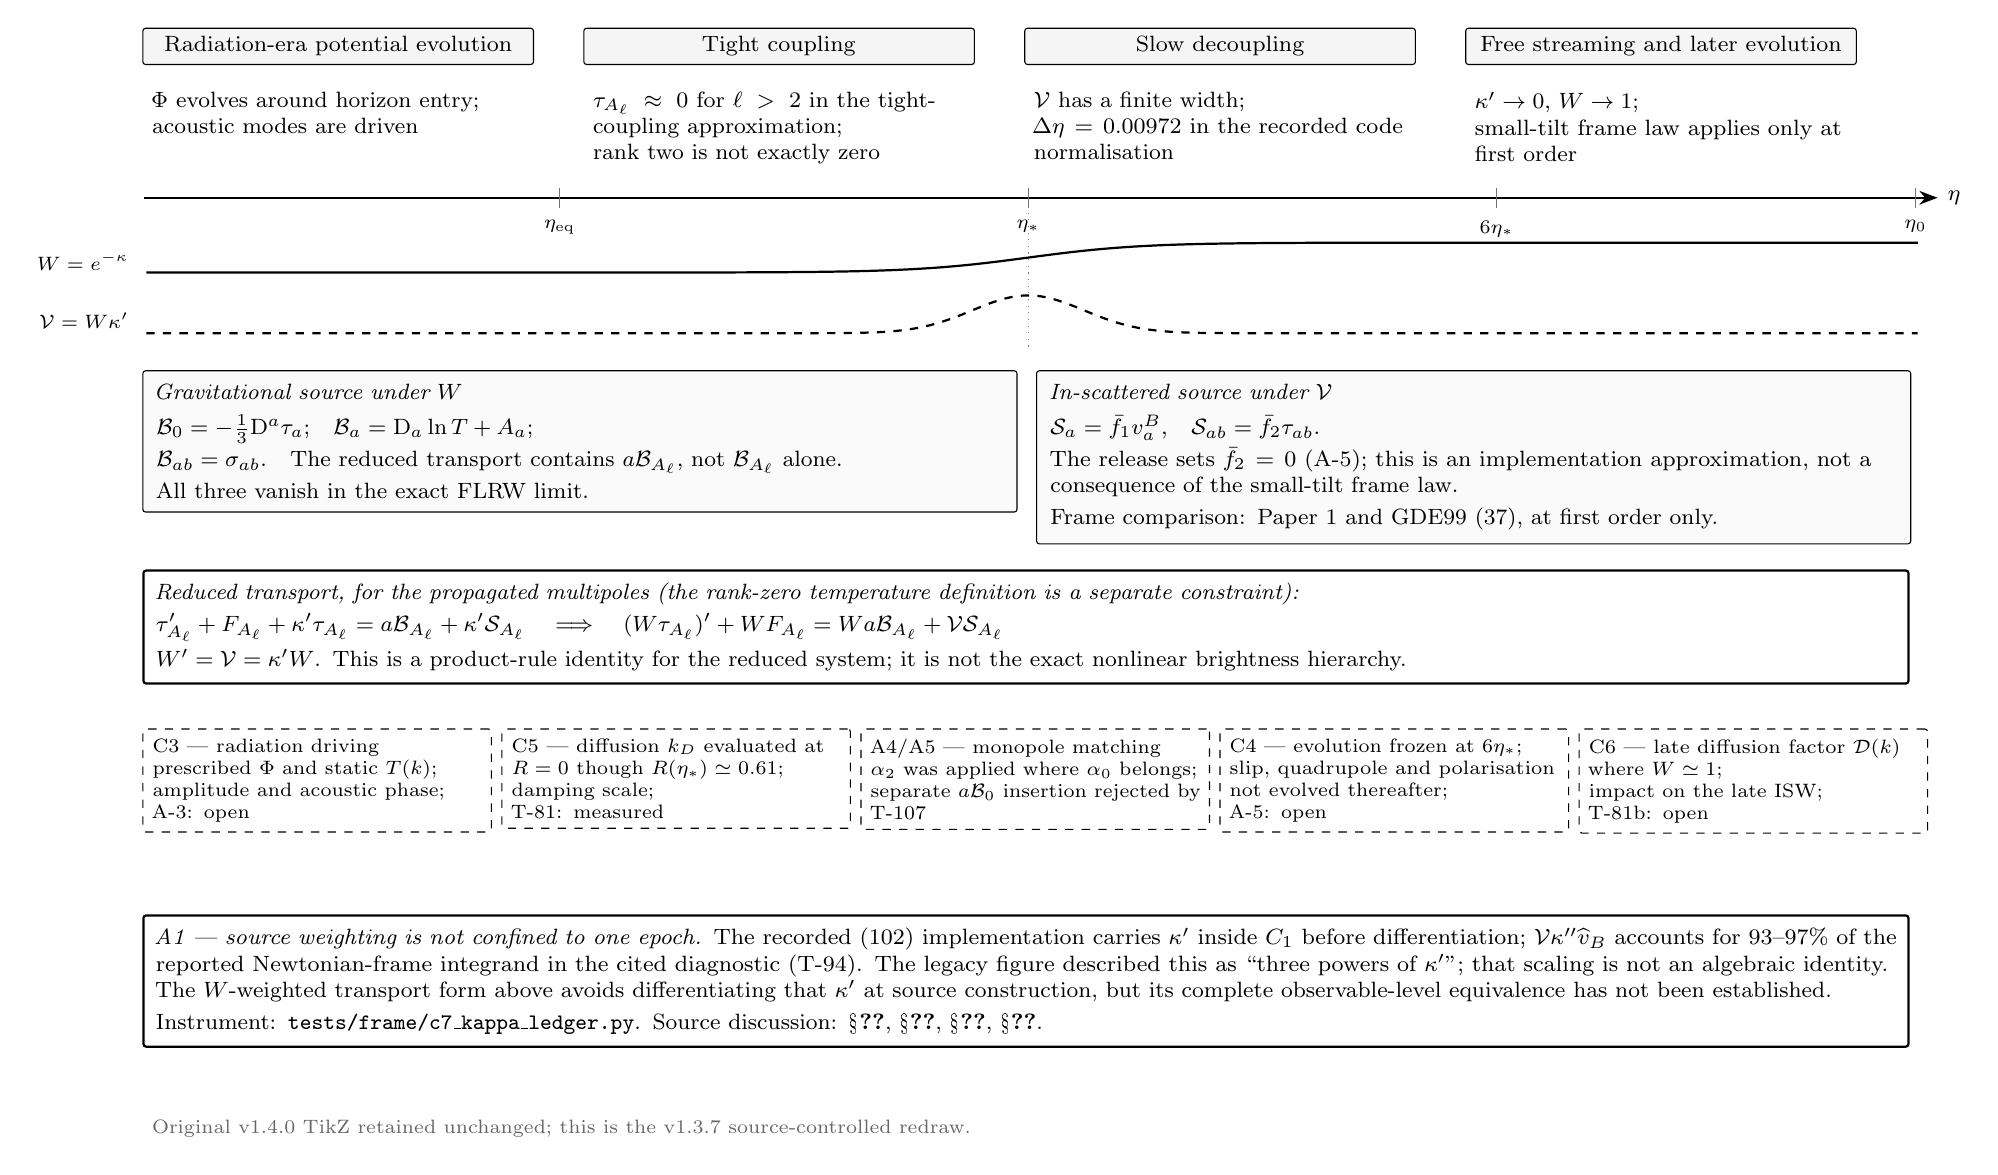
\begin{tikzpicture}[
  x=1cm,y=1cm, font=\footnotesize, >=Stealth,
  epoch/.style={draw,fill=black!4,rounded corners=1pt,minimum height=0.46cm,
                align=center,inner sep=3pt},
  source/.style={draw,rounded corners=1pt,fill=black!2,align=left,
                 anchor=north west,inner sep=5pt,text width=10.75cm},
  check/.style={draw,dashed,rounded corners=1pt,align=left,
                anchor=north west,inner sep=3.5pt,text width=4.18cm,font=\scriptsize},
  rulebox/.style={draw,thick,rounded corners=1pt,align=left,anchor=north west,
                  inner sep=4.5pt,text width=22.1cm},
  tick/.style={black!55},
  small/.style={font=\scriptsize},
]
% Four physical stages.  Equal graph distance does not imply equal conformal time.
\node[epoch,anchor=north west,text width=4.75cm] at (0.10,2.50)
 {Radiation-era potential evolution};
\node[epoch,anchor=north west,text width=4.75cm] at (5.70,2.50)
 {Tight coupling};
\node[epoch,anchor=north west,text width=4.75cm] at (11.30,2.50)
 {Slow decoupling};
\node[epoch,anchor=north west,text width=4.75cm] at (16.90,2.50)
 {Free streaming and later evolution};
\node[anchor=north west,align=left,text width=5.00cm] at (0.10,1.81)
 {$\Phi$ evolves around horizon entry;\\ acoustic modes are driven};
\node[anchor=north west,align=left,text width=5.00cm] at (5.70,1.81)
 {$\tau_{A_\ell}\approx0$ for $\ell>2$ in the tight-coupling approximation;\\ rank two is not exactly zero};
\node[anchor=north west,align=left,text width=5.00cm] at (11.30,1.81)
 {$\mathcal V$ has a finite width;\\ $\Delta\eta=0.00972$ in the recorded code normalisation};
\node[anchor=north west,align=left,text width=5.00cm] at (16.90,1.81)
 {$\kappa'\rightarrow0$, $W\rightarrow1$;\\ small-tilt frame law applies only at first order};
\draw[->,thick] (0.12,0.34)--(22.90,0.34) node[right] {$\eta$};
\foreach \xx/\lab in {5.40/{$\eta_{\rm eq}$},11.35/{$\eta_*$},17.30/{$6\eta_*$},22.62/{$\eta_0$}} {
 \draw[tick] (\xx,0.21)--(\xx,0.47);
 \node[below=1pt,font=\scriptsize] at (\xx,0.21) {\lab};
}
\node[anchor=east,font=\scriptsize] at (0.05,-0.47) {$W=e^{-\kappa}$};
\draw[thick,samples=170,domain=0.15:22.65,smooth,variable=\x]
 plot (\x,{-0.61+0.38/(1+exp(max(-8,min(8,-(\x-11.35)*1.4))))});
\node[anchor=east,font=\scriptsize] at (0.05,-1.22) {$\mathcal V=W\kappa'$};
\draw[thick,dashed,samples=160,domain=0.15:22.65,smooth,variable=\x]
 plot (\x,{-1.38+0.48*exp(-((\x-11.35)*1.0)^2)});
\draw[gray,dotted] (11.35,-1.55)--(11.35,0.25);
% Schematic status is stated in the caption; avoid overprinting the visibility line.
% Source sectors; use the definitions of B_l, and show the separate factor a.
\node[source] at (0.10,-1.85) {\emph{Gravitational source under $W$}\\[3pt]
 $\mathcal B_0=-\tfrac13\mathrm D^a\tau_a$;\quad
 $\mathcal B_a=\mathrm D_a\ln T+A_a$;\\[2pt]
 $\mathcal B_{ab}=\sigma_{ab}$.\quad
 The reduced transport contains $a\mathcal B_{A_\ell}$, not $\mathcal B_{A_\ell}$ alone.\\[2pt]
 All three vanish in the exact FLRW limit.};
\node[source] at (11.45,-1.85) {\emph{In-scattered source under $\mathcal V$}\\[3pt]
 $\mathcal S_a=\bar f_1 v^B_a$,\quad
 $\mathcal S_{ab}=\bar f_2\tau_{ab}$.\\[2pt]
 The release sets $\bar f_2=0$ (A-5); this is an implementation approximation, not a consequence of the small-tilt frame law.\\[2pt]
 Frame comparison: Paper 1 and GDE99 (37), at first order only.};
% The algebraic integrating-factor identity, with rank-0 caveat.
\node[rulebox] at (0.10,-4.38)
 {\emph{Reduced transport, for the propagated multipoles (the rank-zero temperature definition is a separate constraint):}\\[2pt]
 $\displaystyle
  \tau'_{A_\ell}+F_{A_\ell}+\kappa'\tau_{A_\ell}
     =a\mathcal B_{A_\ell}+\kappa'\mathcal S_{A_\ell}
  \quad\Longrightarrow\quad
  (W\tau_{A_\ell})'+W F_{A_\ell}
     =W a\mathcal B_{A_\ell}+\mathcal V\mathcal S_{A_\ell}$\\[2pt]
 $W'=\mathcal V=\kappa'W$. This is a product-rule identity for the reduced system; it is not the exact nonlinear brightness hierarchy.};
% Five original timed diagnostic sites, without promoting a hypothesis to theorem.
\node[check] at (0.10,-6.40)
 {C3 --- radiation driving\\ prescribed $\Phi$ and static $T(k)$;\\ amplitude and acoustic phase;\\ A-3: open};
\node[check] at (4.66,-6.40)
 {C5 --- diffusion $k_D$ evaluated at $R=0$ though $R(\eta_*)\simeq0.61$;\\ damping scale;\\ T-81: measured};
\node[check] at (9.22,-6.40)
 {A4/A5 --- monopole matching\\ $\alpha_2$ was applied where $\alpha_0$ belongs;\\ separate $a\mathcal B_0$ insertion rejected by T-107};
\node[check] at (13.78,-6.40)
 {C4 --- evolution frozen at $6\eta_*$;\\ slip, quadrupole and polarisation not evolved thereafter;\\ A-5: open};
\node[check] at (18.34,-6.40)
 {C6 --- late diffusion factor $\mathcal D(k)$ where $W\simeq1$;\\ impact on the late ISW;\\ T-81b: open};
\node[rulebox] at (0.10,-8.76)
 {\emph{A1 --- source weighting is not confined to one epoch.} The recorded (102) implementation carries $\kappa'$ inside $C_1$ before differentiation; $\mathcal V\kappa''\widehat v_B$ accounts for $93$--$97\%$ of the reported Newtonian-frame integrand in the cited diagnostic (T-94). The legacy figure described this as ``three powers of $\kappa'$''; that scaling is not an algebraic identity. The $W$-weighted transport form above avoids differentiating that $\kappa'$ at source construction, but its complete observable-level equivalence has not been established.\\[2pt]
 Instrument: \texttt{tests/frame/c7\_kappa\_ledger.py}. Source discussion: \S\ref{sec:w-form}, \S\ref{sec:ell-zero-row}, \S\ref{sec:kappa-ledger}, \S\ref{sec:frame-discrepancy}.};
\node[anchor=north west,font=\scriptsize,text=black!60] at (0.1,-11.25)
 {Original v1.4.0 TikZ retained unchanged; this is the v1.3.7 source-controlled redraw.};
\end{tikzpicture}
\captionsetup{width=\linewidth,justification=raggedright,singlelinecheck=false}
\captionof{figure}[Photon history, source weights and 1+3 covariant limitations]{The photon's history and the source-weighting and matching questions in the reconstructed $1+3$ radiation transport. The positions on the conformal-time axis and the opacity curves are schematic. The $\mathcal B_{A_\ell}$ definitions and the first-order frame qualifier follow the published $1+3$ antecedents and Paper~1, while the five numbered diagnostics and A1 are statements about the repository reconstruction, not additional covariant identities. The reduced integrating-factor identity is distinguished from the exact brightness hierarchy. The original Figure~1 TikZ remains available for literal comparison under \texttt{tikz/figure-history-flow-v1.4.0.tex}; the detailed claim and source reconciliation is in \texttt{FIGURE-1-AUDIT-v1.3.7.md}.}
\label{fig:history-flow}
\endgroup
\end{landscape}
\clearpage


\paragraph{The estimate in Figure 1.}
The v1.3.6 diagram also gave
$\tau_{ab}\simeq-(\kappa')^{-1}
[\sigma_{ab}+\mathrm D_{\langle a}v^B_{b\rangle}]$.
It is retained as reported, but its proper/conformal-time conversion remains
open.\footnote{Here $\kappa'$ is a conformal-time rate whereas the unscaled
kinematic tensors use proper-time derivatives. The published tensor
relation has not been independently certified.}
Neither this estimate, the $\bar f_2=0$ approximation nor the proposed
$W$-form is presented as an independently verified consequence of the exact
brightness hierarchy. The accepted original TikZ is retained unchanged.

Figure~\ref{fig:history-flow} is the order this section and
\S\ref{sec:frame-discrepancy} are written in. It is the photon's history and
not a table of contents: each open question is drawn at the conformal time it
acts at, which is what separates the questions that a frame instrument can see
from the questions it cannot.

% ===========================================================================
\subsection{The integration by parts and the invariant assembly}
\label{sec:w-form}

\paragraph{The exact integration by parts.} Done exactly, the integration by
parts carries three terms beyond (102)'s bracket. (102)'s bulk integrand comes
from integrating $\int W\big(C_0K+C_1K'+C_2K''\big)\,\mathrm d\eta$ by parts
onto the coefficients, with kernel $K(\eta)=j_\ell(k\Delta\eta)$ and
$\Delta\eta\equiv\eta_0-\eta$. The weight $W=e^{-\kappa}$ sits inside the
integral, so it is differentiated too, and
$W'=\mathcal V$, $\mathcal V'=(\kappa''+\kappa'^2)W$:
\begin{equation}
  WC_0-(WC_1)'+(WC_2)''
  \;=\;\underbrace{W\big(C_0-C_1'+C_2''\big)}_{\text{(102)'s bracket}}
  \;-\;\mathcal VC_1\;+\;2\mathcal VC_2'\;+\;\mathcal V'C_2 .
  \label{eq:byparts}
\end{equation}


The integrations by parts, including their boundary terms, are
\begin{align}
 \int_{\eta_*}^{\eta_0}WC_1K'\,\mathrm d\eta
   &=\big[WC_1K\big]_{\eta_*}^{\eta_0}
      -\int_{\eta_*}^{\eta_0}(WC_1)'K\,\mathrm d\eta,\\
 \int_{\eta_*}^{\eta_0}WC_2K''\,\mathrm d\eta
   &=\big[WC_2K'-(WC_2)'K\big]_{\eta_*}^{\eta_0}
      +\int_{\eta_*}^{\eta_0}(WC_2)''K\,\mathrm d\eta.
 \label{eq:v135-byparts-steps}
\end{align}
With $\kappa(\eta)=\int_\eta^{\eta_0}\kappa'(s)\,\mathrm ds$,
$W'=\kappa'W=\mathcal V$ and
$W''=\mathcal V'=(\kappa''+\kappa'^2)W$. Consequently
$(WC_1)'=WC_1'+\mathcal VC_1$ and
$(WC_2)''=WC_2''+2\mathcal VC_2'+\mathcal V'C_2$.
Substitution reproduces \eqref{eq:byparts} term by term, without making a
frame choice or dropping a boundary. The difference between that exact
identity and a published projected solution can be assessed only after
establishing the projected source and endpoint conventions from the published
paper. Equality of these two integration-by-parts expressions alone does not
establish Eq.~(102).\footnote{The full line-of-sight comparison with the
published journal Eq.~(102), including projected boundary normalisation,
has not been independently closed. This algebra tests the transformation of
a specified integrand, not the derivation of that integrand from the exact
brightness hierarchy.}



\paragraph{The two weights.} The two weights are not interchangeable, and
the kernel each leaves behind separates them. \eqref{eq:byparts} puts the
bracket $C_0-C_1'+C_2''$ under $W$ and leaves $-\mathcal VC_1$,
$2\mathcal VC_2'$ and $\mathcal V'C_2$ beside it. Carrying that bracket under
$\mathcal V$ instead is B-17's discrepancy~(i), and the consequence is not a
change of size. Take any coefficient $C$ and apply the
product rule under each weight in turn:
\begin{align}
 \int_{\eta_*}^{\eta_0}WCK'\,\mathrm d\eta
   &=\big[WCK\big]_{\eta_*}^{\eta_0}
     -\int_{\eta_*}^{\eta_0}\mathcal VCK\,\mathrm d\eta
     -\int_{\eta_*}^{\eta_0}WC'K\,\mathrm d\eta,
   \label{eq:weight-w-byparts}\\
 \int_{\eta_*}^{\eta_0}\mathcal VCK'\,\mathrm d\eta
   &=\big[\mathcal VCK\big]_{\eta_*}^{\eta_0}
     -\int_{\eta_*}^{\eta_0}\mathcal V'CK\,\mathrm d\eta
     -\int_{\eta_*}^{\eta_0}\mathcal VC'K\,\mathrm d\eta .
   \label{eq:weight-v-byparts}
\end{align}
Both boundary terms vanish. $\big[WCK\big]$ does so because $W(\eta_0)=1$
against $j_\ell(0)=0$ for $\ell\ge1$ at the top and $W\to0$ at the bottom;
$\big[\mathcal VCK\big]$ does so because the visibility vanishes at both
ends. What differs is the kernel each line puts in the boundary's place,
and the two differ in the one property that matters here:
\begin{equation}
  \int_{\eta_*}^{\eta_0}\mathcal V\,\mathrm d\eta=1,
  \qquad
  \int_{\eta_*}^{\eta_0}\mathcal V'\,\mathrm d\eta
    =\big[\mathcal V\big]_{\eta_*}^{\eta_0}=0 .
  \label{eq:kernel-weights}
\end{equation}

\paragraph{Terms at $K'$.} A term that reaches the kernel through $K'$
yields no primary when it is carried at the visibility, and the claim is
restricted to $K'$. \eqref{eq:kernel-weights} is the argument. A kernel of
unit weight reproduces its integrand at the deposit,
$\int\mathcal Vf\,\mathrm d\eta\to f(\eta_\ast)$, which is the
$\int\mathcal V=1$ collapse this document uses throughout and is what a
primary anisotropy \emph{is}: the source at last scattering, carried intact
to one epoch. A kernel of \emph{zero} weight reproduces nothing. Integrating
\eqref{eq:weight-v-byparts}'s replacement against a smooth $f$ gives
$\int\mathcal V'f\,\mathrm d\eta\to-f'(\eta_\ast)$: it acts as a derivative
rather than as a sample. Of two terms reaching the kernel through $K'$, the
one carried at $W$ therefore yields a primary and the one carried at
$\mathcal V$ the derivative of one. A term carried at $\mathcal V$ against $K$
itself is untouched by this and samples correctly; that is the Sachs--Wolfe
channel. Editions before 2 November stated the result without the restriction
to $K'$, and so claimed it for the monopole too.

\paragraph{The weights and the missing series.} The kernel weights do not
explain the missing series, as editions from 31 October to 2 November said
they did. A derivative of a primary is a primary displaced by half a period: $\sin(kr_s)$ has as many
zeros as $\cos(kr_s)$, so a kernel that differentiates moves a peak series and
cannot erase one. Those editions argued that the factor of $k$ a derivative
brings tilts rather than features, and concluded an envelope; the conclusion
does not follow. The identities
\eqref{eq:weight-w-byparts}--\eqref{eq:kernel-weights} stand as mathematics,
and the account of the series built on them is withdrawn, with the
attribution that went with it. The term measured at $93$--$97\%$ of (102)'s
bulk, $\mathcal V\kappa''\hat v_B$, belongs to the admissibility
condition of \S\ref{sec:assembly-rederived} and not to the weight: $C_1$ holds
$\kappa'\hat v_B$ by (90), so differentiating $C_1$ under either weight
produces $\kappa''\hat v_B$. It is the bulk face of the operation whose
boundary face is $\kappa'\hat v_B$ standing in the Sachs--Wolfe slot, and no
choice of weight removes it.

\paragraph{The two falsifiers.} The series is not a weight question, and both
registered falsifiers say so. Editions before 2 November named
\texttt{bracket\_\allowbreak{}all\_\allowbreak{}at\_\allowbreak{}w} as the
falsifier and predicted that it returns a peak series. The prediction was
withdrawn on 2 November as answerable before it was made: D32 had run that
configuration on 25 October, and T-143 says why it cannot localise --- carried at $W$ the bracket is integrated along the whole ray,
where $C_0$ and $C_2$ grow by a factor of $33$ while $W$ falls only to
$0.368$. Carried through a full $C_\ell$ since, it returns one maximum and no
interior minimum between $\ell=300$ and $900$ on each background tried, so
the prediction failed. Its replacement,
\texttt{isw\_\allowbreak{}only\_\allowbreak{}at\_\allowbreak{}w}, was
registered as \emph{the spectrum stays localised at recombination and carries
at least one interior minimum between $\ell=300$ and $\ell=900$}, with a
second falsifier, \emph{localised but still an envelope}. Run on PLANCK
through F9's spectrum as then drawn, from (102), its CDM-frame column is the
released column of (102), one maximum, at $\ell_A$, and no trough to
$\ell=990$, and the second falsifier fires as written: the absence of the
secondaries is not a weight question. Neither run is yet among this bundle's released diagnostics.

\paragraph{The measurements kept.} The measurements offered for the
withdrawn account stand as measurements. The first peak of (102) as built sits
at $0.9994\,\ell_A$; its reading as one surviving snapshot of the undriven
source goes with the account (\S\ref{sec:first-peak}). (102)'s spectrum under
\texttt{split\_by\_parts} rises to one maximum and decays with no trough. D42
separates each coefficient from its pedestal with a running mean
one acoustic period wide, a filter with a zero at the acoustic frequency that
cannot leak the oscillation into the pedestal: $\hat v_B$ and $-C_1$ carry the
wave at $26.5\%$ and $22.1\%$ modulation, and $C_0$, in the CDM frame, at
$0.12\%$. Read directly, none of the three crosses zero below $k=600$: each
oscillates on a pedestal larger than the oscillation.

\paragraph{The rank-zero frame rule.} The frame rule for rank zero is
measured. Under a change of frame $C_0$ shifts by $+kv/3$ and $\tfrac k3\tau_1$ by $-kv/3$, so only their
sum is a physical object. The sum agrees between the Newtonian and CDM frames
to $2.1\times10^{-14}$ over the visibility window for $k=2$--$600$, which is
double-precision roundoff, while $C_0$ alone is $0$ in the Newtonian frame and
$185$ in the CDM frame at $k=300$ (D42). $C_0$ is built from the
shear, which vanishes in a shear-free frame, so there the bracket \emph{is}
$\tfrac k3\tau_1$, the photon dipole relative to a shear-free $u^a$, and it
crosses zero four times below $k=400$, near $106$, $174$, $266$ and $340$
(D42). The source carries the acoustic wave, and a statement about $C_0$ alone
is a statement about a frame.

\paragraph{The frame conditions.} At first order
a change of frame moves only the dipole, so for every observer the
multipoles with $\ell\ge2$ of $\int_0^{\eta_0}W\{C_0K+C_1K'+C_2K''\}\,
\mathrm d\eta$ must not move. With $W(0)=0$, $W(\eta_0)=1$,
$j_\ell(0)=\delta_{\ell0}$ and $j_\ell'(0)=\tfrac13\delta_{\ell1}$, that
holds exactly when the shift of the integrand is a total derivative,
\begin{equation}
  W\big\{\Delta C_0\,K+\Delta C_1\,K'+\Delta C_2\,K''\big\}
  =\frac{\mathrm d}{\mathrm d\eta}\Big[W\big(\alpha K+\beta K'\big)\Big],
  \label{eq:frame-total-derivative}
\end{equation}
which with $W'=\kappa'W$ is three matching conditions: $\Delta C_2=\beta$,
$\Delta C_1=\kappa'\beta+\beta'+\alpha$ and $\Delta C_0=\kappa'\alpha+\alpha'$.
A change of frame is kinematic and cannot depend on the scattering history,
and $C_0$ holds no rate, so $\alpha=0$. Split by rate content,
$C_1=C_1^{\rm grav}+C_1^{\rm scatt}$ with $C_1^{\rm scatt}=-\kappa'\hat v_B$,
the conditions are
\begin{equation}
  \Delta C_0=0,\qquad
  \Delta C_1^{\rm scatt}=\kappa'\,\Delta C_2,\qquad
  \Delta C_1^{\rm grav}=\Delta C_2' .
  \label{eq:frame-conditions}
\end{equation}
Rank zero is frame-invariant alone, the scattering half of rank one pairs
with $C_2$, and the gravitational half pairs with $C_2'$. No
$\int\mathcal V=1$ collapse enters, so the conditions hold at the
visibility's finite width. The second is T-82: $\hat v_B+C_2$ agrees between
the frames to machine precision, and it holds. The first fails, by D42's $0$
against $185$. The third fails as well, and it can be
read off this bundle's own transformation laws. The moving projector shifts
$\delta T$ by $-\mathcal Hv/k$, the CDM frame sets $\tilde\Phi_A=0$, and
$v'+\mathcal Hv=-k\Phi_A$, so $\delta T+\Phi_A$ shifts by $+v'/k$ and
$C_1^{\rm grav}=-(\delta T+\Phi_A)$ by $-v'/k$; $C_2=v/k$ makes
$\Delta C_2'=+v'/k$, so the third condition fails by exactly $2C_2'$.

\paragraph{The lost series.} (102)'s integration by parts does two things that no weight undoes. It carries
$\kappa'\hat v_B$ into the Sachs--Wolfe slot and, one derivative on,
$\mathcal V\kappa''\hat v_B$ into the bulk; and by integrating the rank-two
term by parts twice it separates $C_2$ from $\hat v_B$, the pair the second
condition of \eqref{eq:frame-conditions} binds. In a shear-free frame $C_2$
vanishes and the separation is invisible. In the CDM frame $\hat v_B$ carries
$-v/k$, the frame velocity, which is smooth in $k$; separated from $C_2$ and
multiplied by $\kappa'$ it is a pedestal under the oscillating monopole, and
the series does not survive it. The missing series and the frame
discrepancy of \S\ref{sec:frame-discrepancy} are therefore one defect.

\noindent
What this rules out is a repair at the boundary. (102)'s boundary scalar
$(C_2'-C_1)\,j_\ell$ is not a free choice of sign: \eqref{eq:byparts} forces
it from $+C_2K''$, so printing $-C_2'$ there would make the collapsed boundary
frame-invariant and the boundary no longer the boundary of its own integrand.
The defect is upstream, in how the gravitational coefficients carry the
frame, and Paper~1's own source equation names it. Its linear redshift
source is
\begin{equation}
  \mathcal B^{\rm P1}(x,e)\simeq+\tfrac13\mathrm D^a\tau_a
    -(\mathrm D_a\ln T+A_a)e^a-\sigma_{ab}e^ae^b=-\mathcal B(x,e),
  \label{eq:paper1-source}
\end{equation}
with the Thomson term $+\sigma_{\rm T}n_e\bar f_1e^av^B_a$ beside it on the
right-hand side. Two features of it are absent from this bundle's
coefficients. The rank-one gravitational source enters with the opposite
sign to the Thomson Doppler term, as it does in \emph{Annals~II}'s own
Eq.~(67) and in that equation's rank-one mode form, its Eq.~(13). The
rank-one row of the matching that the frame conditions select is
$kC_1=a\mathcal B_1-\kappa'v_B$, with $a\mathcal B_1=k(\delta T+\Phi_A)$
(\S\ref{sec:source-derivatives}), where (89) prints
$-(a\mathcal B_1+\kappa'v_B)$ and the coefficients are built from it. With
Paper~1's source in $\mathcal B_1$'s place,
$a\mathcal B^{\rm P1}_1=-k(\delta T+\Phi_A)$, the printed row is the selected
one, and that is how the code carries it. And the rank-zero source is
carried: $\mathcal B^{\rm P1}_0=\tfrac13\mathrm D^a\tau_a=-\mathcal B_0$ enters
$C_0$ as $-a\mathcal B_0=\tfrac k3\tau_1$, where the coefficients drop it
(\S\ref{sec:ell-zero-row}).\footnote{The frame conditions fix the row, not
which printed sign is at fault. Against \emph{Annals~II}'s own Eq.~(13), its
mode form (71) carries the Thomson term with the wrong sign, and (89) repeats
(71). The selected row also carries, at rank one, the sign of the kernel's
derivative, $K'=-k\,j_\ell'$ for $K=j_\ell\big(k(\eta_0-\eta)\big)$, which
ranks zero and two do not: against \emph{Annals~II}'s source $\mathcal S_B$,
as (12) and (13) fix it at ranks two and one and (71) at rank zero, the
selected row is $-\mathcal S_B$ at rank one and $+\mathcal S_B$ at ranks zero
and two. The two
compound to the one difference above, the sign of $a\mathcal B_1$.} Scored
symbolically against this bundle's own transformation laws, with the matching
(89) as built, the three conditions of \eqref{eq:frame-conditions} read:
\begin{center}\small
\begin{tabular}{@{}lcccc@{}}
\toprule
coefficients & rank zero & scattering & gravitational & by-parted $K$ coefficient \\
\midrule
as built & $kv/3$ & $0$ & $-2v'/k$ & frame-dependent \\
rank-one sign corrected alone & $kv/3$ & $0$ & $0$ & frame-dependent \\
$a\mathcal B_0$ carried alone (T-105) & $0$ & $0$ & $-2v'/k$ & frame-dependent \\
both, as \eqref{eq:paper1-source} & $0$ & $0$ & $0$ & invariant, identically \\
\bottomrule
\end{tabular}
\end{center}
Both corrections are needed together, and neither works alone. That is why
T-105 was refuted when it was tried by itself: with the rank-one sign as built, $-C_1'$
carries $+\tfrac k3\tau_1$ and the restored $-a\mathcal B_0$ doubles it, which
is the $98.5\%$ criterion~5b caught; with the sign of
\eqref{eq:paper1-source}, $-C_1'$ carries $-\tfrac k3\tau_1$ and
$-a\mathcal B_0$ cancels it. In a shear-free frame the $W$-carried
gravitational content of the bracket is then $-(\Phi_A'-\Phi_H')$, the
integrated Sachs--Wolfe term, with no photon dipole riding along the ray. The
transformation laws for $\delta T$ and $\Phi_A$ are right, and (102)'s
$+C_2'$ stands. The frame test cannot see the relative sign between the
$j_\ell$ and $j_\ell'$ slots, since each is invariant on its own;
\eqref{eq:paper1-source} and the matching (89) fix it, as the scoring below
shows.

\paragraph{The registered repair.} On 3 November, before it was built, the
repair was registered as follows. Build
$a\mathcal B_1$ with the sign of \eqref{eq:paper1-source}, at the one place it
is defined, and carry $a\mathcal B_0$ in $C_0$ with it and never without it;
score \eqref{eq:frame-conditions} on the coefficients before any spectrum is
read. Registered: \emph{(a)} the three conditions hold to the integrator's
tolerance at every mode; \emph{(b)} in the Newtonian frame the $W$-carried
gravitational content is $-(\Phi_A'-\Phi_H')$ and $\tfrac k3\tau_1$ cancels;
\emph{(c)} the exact identity, the bracket at $W$ with its visibility terms,
returns $C_\ell$ at $\ell\ge2$ identical in the two frames, and on
Einstein--de~Sitter, where the potentials are constant and there is no late
effect to carry, it no longer puts power late; \emph{(d)} the assembly that
keeps $\kappa'$ out of every derivative and $\hat v_B$ with $C_2$ carries a
peak series in both frames, identical at $\ell\ge2$. If \emph{(d)} fails while
\emph{(a)}--\emph{(c)} hold, the loss of the series is not a frame defect, and
the admissibility condition is what remains.

\paragraph{The assembly.} Write
$G\equiv C_1^{\rm grav}-C_2'$, the combination the third condition of
\eqref{eq:frame-conditions} makes frame-invariant. Then, exactly,
\begin{equation}
  W\{C_0K+C_1K'+C_2K''\}
  =W\,(C_0-G')\,K-\mathcal V\,G\,K-\mathcal V\,(\hat v_B+C_2)\,K'
   +\frac{\mathrm d}{\mathrm d\eta}\Big[W\big(GK+C_2K'\big)\Big],
  \label{eq:assembly-invariant}
\end{equation}
and the total derivative projects onto $\ell\le1$ alone, since $W(0)=0$,
$K(\eta_0)=\delta_{\ell0}$ and $K'(\eta_0)=-\tfrac k3\delta_{\ell1}$. Every
slot is frame-invariant on its own: $C_0$ by the first condition, $G$ and so
$G'$ by the third, $\hat v_B+C_2$ by the second. No coefficient holding a
rate is differentiated, since the scattering half of $C_1$ is never
integrated by parts and $C_2$ holds no rate; and no rank-two partner is
separated from its rank-one half. That second property is the
admissibility condition's companion, and it is checkable in the tree as the
rate condition is: a rank-two term may be integrated by parts once, onto the
slot its rank-one partner occupies, and not twice.
\eqref{eq:assembly-repaired} is the rank-one restriction of
\eqref{eq:assembly-invariant}. In a shear-free frame $C_2=0$ and
$G=C_1^{\rm grav}$, so $\tfrac k3\tau_1$ cancels from $C_0-G'$ and
\eqref{eq:assembly-invariant} is the Sachs--Wolfe deposit at $j_\ell$, the
Doppler deposit at $j_\ell'$ and the integrated Sachs--Wolfe term at $W$:
the three terms of the standard line-of-sight solution. Collapsed onto the
visibility it is (102)'s boundary with the rank-one sign of
\eqref{eq:paper1-source}, and with $\kappa'\hat v_B$ taken out of the
$j_\ell$ slot and returned, as $\hat v_B$, to the $j_\ell'$ slot it came
from. The difference of the two sides of \eqref{eq:assembly-invariant} is
zero in exact symbols, for arbitrary $W$, $\kappa'$ and coefficients.

\paragraph{The registrations scored.} D44, released on 4 November, scores
the four registrations on Einstein--de~Sitter, $\Lambda$CDM and
\texttt{PLANCK\_MODEL}: at the coefficients for $k=2$ to $400$, and in the
transfer on F9's $k$ grid to $k=1500$. Registration \emph{(a)} holds. With
Paper~1's signs the largest relative frame shift over the window
$W>10^{-10}$ is at most $3.3\times10^{-13}$ at rank zero,
$2.6\times10^{-13}$ in the scattering condition and $6.1\times10^{-16}$ in the
gravitational one, while as built the rank-zero and gravitational conditions
fail at order one, $1.0$ and $1.4$--$1.8$. Registration \emph{(b)} holds: in
the Newtonian frame the $W$-carried gravitational content equals
$-(\Phi_A'-\Phi_H')$ to $4.6\times10^{-16}$, against $18$ to $2\times10^{11}$
as built, so $\tfrac k3\tau_1$ cancels.

Registration \emph{(c)} was printed against the bracket at $W$ with its
visibility terms. On 3 November, before the run, it was restated as a
statement about the uncollapsed identity, which is the three-slot assembly
term for term, because the collapsed form keeps
$-\kappa'(\eta_*)\Delta C_2(\eta_*)$ at the boundary and drops the bulk
partners that cancel it. In that form it holds. The three slots give one
$C_\ell$ in both frames to $4.2\times10^{-14}$, and each mode to
$2.5\times10^{-8}$, below D44's stated thresholds of $10^{-12}$ for $C_\ell$
and $10^{-6}$ per mode; and on
Einstein--de~Sitter the integrated slot carries a fraction
$2.7\times10^{-23}$ of the power, so no power is put late where the
potentials are constant. A competing prediction, that this slot would carry
late power there, is refuted. The collapsed form, measured
alongside, differs between the frames at order one, $1.1$ to $1.6$, as the
restatement said it would.

Registration \emph{(d)} holds on Einstein--de~Sitter and fails on
\texttt{PLANCK\_MODEL}. The three slots are identical in the two frames on
every background. On Einstein--de~Sitter, with $\ell_A=190.6$, they put
maxima of $D_\ell$ at $\ell=165$ and $495$ and a trough at $360$: an interior
minimum between $\ell=300$ and $900$, the criterion carried from
3 November, with the first maximum at $0.87\,\ell_A$. On $\Lambda$CDM they put
maxima at $150$ and $450$ with no trough that meets the shared prominence
rule. On \texttt{PLANCK\_MODEL} they put a single maximum, at $0.71\,\ell_A$,
and no trough, where CAMB and CLASS put maxima at $206$, $491$, $730$, $1014$
and $1276$ ($1277$ for CLASS). The registration reads a failure of \emph{(d)} with
\emph{(a)}--\emph{(c)} holding as a loss of the series that is not a frame
defect, and names the admissibility condition as what remains. The first half
holds on \texttt{PLANCK\_MODEL}. The second does not apply, because the
assembly scored satisfies the admissibility condition by construction. What
separates \texttt{PLANCK\_MODEL} from the backgrounds that carry the series is
not yet scored. D45 measures where the slots cancel, and no pair cancels at
$\ell=100$--$400$: there the integrated slot is $1$--$5\%$ of $C_\ell$ and twice
the cross-spectrum of the Sachs--Wolfe and integrated slots adds $11$--$16\%$,
in phase. D44's $2.1$ is the integrated slot's auto-spectrum at $\ell=5$, and
from $\ell=2$ to $10$ twice that cross-spectrum runs from $-1.9$ to $-3.1$ of
the total, against $-0.12$ at $\ell=2$ on $\Lambda$CDM. The cause is in the
potential both slots read, and it is A-3's. \texttt{PLANCK\_MODEL}'s
background carries radiation, so $D/a$ falls by $7\%$ before $\eta_*$ and by
$10\%$ more by matter domination, while the monopole starts from the matter-era
adiabatic value $-\tfrac23\Phi_A$ and the radiation-era potential
\eqref{eq:radiation-potential} is not wired: the radiation era is half
present. The Sachs--Wolfe source at last scattering is then $0.187$ against
$\Phi_A/3=0.310$, with $0.535$ in the integrated slot. \texttt{LCDM\_MODEL},
whose background carries no radiation, returns $\Phi_A/3$ to three figures,
$0.3331$, and $2\Delta\Phi=0.442$ in the integrated slot. F9's
\texttt{PLANCK\_MODEL} curve below $\ell\simeq30$, its dip near $\ell=5$
included, is therefore the incomplete radiation era of A-3 and not a
prediction of v1.3.0, and its bump at $\ell\simeq7$--$12$ is the start rule
that comes with it, which gives a band of modes the matter-era condition on
a potential that has already decayed (T-192). The radiation era is
v1.4.0's, constructed in \S\ref{sec:a3-construction}.

\paragraph{The sum-back.} The sum-back asked for on 3 November, the three
slots and the total derivative against the direct integral mode by mode,
closes. D44 had found the direct integral and its five-slot form apart from
the three slots at order one in the CDM frame. D45 sums the three slots and
the end points against a direct quadrature built from the same arrays, in
both frames, for $k=2$ to $1500$, and their difference falls by a factor of
$4.00$ when the $\eta$ step halves, in every band. It is quadrature, and it is
the direct integral's: under the halving the slots move by at most
$6\times10^{-5}$ and the direct integral by $5\times10^{-2}$ to $8\times10^2$.
Five slots against three in the CDM frame is the same quadrature. The one
floor that does not fall is T-191, $\int\mathcal V=0.99914$, because the
visibility is interpolated apart from the opacity whose derivative it is;
with $\mathcal V=W'$ it goes. An evaluation independent of the slots now
confirms their weights.

\paragraph{The $C_1^{\rm grav}$ under $\mathcal V$.} The identity is an
integration by parts of one function, so the $C_1^{\rm grav}$ under
$\mathcal V$ and the derivative under $W$ have to be one function and its
derivative. F9 in v1.3.0 pairs the oscillator's stored $C_1^{\rm grav}$ under
$\mathcal V$ with (106) under $W$. The stored moment belongs under
$\mathcal V$: the Sachs--Wolfe slot is the boundary value
$(\delta T+\Phi_A)(\eta_*)$, the solution of the pair (152)--(153) that this
bundle integrates and the oscillator's gates certify
(\S\ref{sec:oscillator}). (106) is that solution's exact derivative on the
grid the pair is integrated on. The released solver runs with
\texttt{expansion\_coupling=False}, which drops the $-\mathcal H\Phi_A$ of
(153) as (154) does, so that in the Newtonian frame
$(\delta T+\Phi_A)'=\Phi_A'-\Phi_H'+\tfrac k3\tau_1$, and with
\texttt{A\_B1\_PRIME\_EXPANSION\_TERMS=False}, the comoving-$k$ convention of
T-67 rather than a dropped term, (106) gives
$(a\mathcal B_1)'=k(\Phi_A'-\Phi_H')+\tfrac{k^2}3\tau_1$, the same expression
term for term. Off that grid the two differ. The stored moments are held
before each mode's start and after the tight-coupling window, and there (106)
is the pair's right-hand side evaluated on the held moments, which is what $W$
needs. Since (106) and $C_0$ are built from one $\tau_1$, the $\tfrac k3\tau_1$
of $-a\mathcal B_0$ in $C_0$ cancels the one in (106) identically: in the
Newtonian frame $C_0-G'=-(\Phi_A'-\Phi_H')$ to $3\times10^{-16}$, inside the
window and past it, as the registered condition \emph{(b)} requires. The
stored moment differentiated on the grid, D45's option (ii), misses
\emph{(b)} by $0.09$ to $0.25$ inside the window, where it is the derivative
of a linear resample, and by order one past it, where it leaves the held
dipole under $W$ along the whole path. It serves D45 as a control on the
sum-back, in which both sides read the same arrays, and not as the pairing.

(106) integrated from the line-of-sight grid's start does not return the
stored moment at last scattering: the two differ by $4\times10^{-4}$ of the
transfer on $\Lambda$CDM and by $1.3\times10^{-2}$ on \texttt{PLANCK\_MODEL}
at $k\le100$. On \texttt{PLANCK\_MODEL} the difference is the start rule's
(T-192). Each mode starts where $kr_s=\varepsilon$, or at the table's first
point if it never reaches it, on the matter-era condition
$\delta T=-\tfrac23\Phi_A$, $\tau_1=0$. For $2.7<k<5.4$ that start falls after
the potential has begun to decay (A-3), and before it the stored moments are
the interpolation's left fill while (106) integrates the decay through them.
Raising the acoustic grid from $24$ to $96$ points per period moves the
difference by a factor of $1.00$, and halving the line-of-sight step moves it
by $1.00$, so it belongs to neither grid; anchoring the reconstruction at each
mode's own start takes the difference between the two moments to
$2$--$9\times10^{-5}$. On $\Lambda$CDM, whose potential is constant until
$\Lambda$, the start rule does not act, and the $4\times10^{-4}$ there is not
yet attributed. The start rule acts inside the slots as well: on
\texttt{PLANCK\_MODEL} the Sachs--Wolfe source at last scattering jumps from
$0.185$ at $k=2.7$ to $0.296$ at $k=2.8$, and F9 carries a bump at
$\ell\simeq7$--$12$, inside the region v1.3.0 already gives to A-3. The start
and the initial condition are redefined with the radiation era. v1.3.32 and
v1.3.33 gave the difference to $-\mathcal H\Phi_A$, which neither expression
contains. Whether the oscillator should carry $-\mathcal H\Phi_A$ at all is a
question about the oscillator rather than the pairing, and is not settled
here.

\paragraph{The relative sign between slots.} D44 probes the relative sign
between slots, which no frame test can see, by reversing the Doppler slot; the
result is again frame-invariant, with the \texttt{PLANCK\_MODEL} maximum at
$0.78\,\ell_A$. That configuration is the slot decomposition of coefficients
that satisfy all three frame conditions but not (89). With $C_2$ reversed,
(89) ties $C_0$ to the same $a\mathcal B_2$ and requires
$\Delta C_0=-\tfrac23kv$, so the first condition fails. The matching therefore
fixes the sign that the frame test cannot, and the reversed run is context
rather than a candidate.

\paragraph{Both endpoints of the projected identity.}
For this calculation alone, define the pre-integrated object
\begin{equation}
 I_\ell=\int_{\eta_*}^{\eta_0}\!\mathrm d\eta\;
 W(\eta)\{C_0K+C_1K'+C_2K''\},\qquad
 K(\eta)=j_\ell\big(k(\eta_0-\eta)\big).
 \label{eq:v136-preintegrated}
\end{equation}
The prime on $K$ denotes \emph{conformal time} differentiation;
$j_\ell'$ below denotes derivative with respect to its argument.
Since $k=k_{\rm com}$ is constant,
\begin{equation}
 K'=-k j_\ell'(x),\qquad K''=k^2j_\ell''(x),\qquad
 j_\ell'(x)=\frac{\ell}{2\ell+1}j_{\ell-1}(x)
                 -\frac{\ell+1}{2\ell+1}j_{\ell+1}(x),
 \quad x=k(\eta_0-\eta).
 \label{eq:v136-kernel-derivative}
\end{equation}
The two separate integration-by-parts lines in
\eqref{eq:v135-byparts-steps} therefore give, without assuming that an
endpoint vanishes,
\begin{align}
 I_\ell={}&\left[WC_1K+WC_2K'-(WC_2)'K\right]_{\eta_*}^{\eta_0}
 \\&+\int_{\eta_*}^{\eta_0}\!\mathrm d\eta\;
 \left[WC_0-(WC_1)'+(WC_2)''\right]K.
 \label{eq:v136-complete-endpoints}
\end{align}
For $\ell\ge2$, $j_\ell(0)=j_\ell'(0)=0$, so the upper
endpoint is zero \emph{provided the coefficient products remain finite}.
The lower endpoint contributes with the opposite sign of the bracket,
therefore
\begin{align}
 E_{*,\ell}&=\left[(WC_2)'-WC_1\right]_*j_\ell(x_*)
       +k[WC_2]_*j_\ell'(x_*)\\
 &=W_*\left[C_2'-C_1+\kappa'_* C_2\right]_*
                  j_\ell(x_*)
       +kW_*C_{2*}j_\ell'(x_*).
 \label{eq:v136-lower-endpoint}
\end{align}
Here $W_*\equiv W(\eta_*)$, $x_*\equiv k(\eta_0-\eta_*)$,
$W'=\kappa'W$; the subscript on the square bracket means all its
terms are evaluated at $\eta_*$. For $\ell=1$ the upper derivative
$K'(\eta_0)=-k/3$ is \emph{not} zero, and for $\ell=0$
$K(\eta_0)=1$; these require their own endpoint accounting.

The boundary in \eqref{eq:v136-lower-endpoint} has two pieces that
cannot be inferred from the published display of (102) by inspection:
the factor $W_*$ and the additional product derivative
$\kappa'_*C_{2*}$ in the scalar slot. Their presence follows from
\emph{the stipulated pre-integrated expression}
\eqref{eq:v136-preintegrated}, not automatically from the published
Boltzmann hierarchy. Whether the actual source in the published
integral solution is \eqref{eq:v136-preintegrated} is the independent
physics question.\footnote{The optical-depth-weighted source and boundary
normalisation of published \emph{Annals~II}, Eq.~(102), have not been
established from the journal pages. Equations
\eqref{eq:v136-complete-endpoints}--\eqref{eq:v136-lower-endpoint}
verify an exact identity for the stated pre-integrated object; they
do not by themselves supply a correction to Eq.~(102) or to the
physical CMB spectrum.}

\paragraph{A time-dependent diffusion factor.}
If the assumed pre-integrated source instead carries a multiplicative
factor $\mathcal D(\eta,k)$, set $P=W\mathcal D$ in
\eqref{eq:v136-preintegrated}. The exact bulk bracket is then
$PC_0-(PC_1)'+(PC_2)''$ and the boundary is obtained from
\eqref{eq:v136-complete-endpoints} by replacing $W$ with $P$.
The derivatives that must be retained are
\begin{equation}
 P'=W'\mathcal D+W\mathcal D',\qquad
 P''=W''\mathcal D+2W'\mathcal D'+W\mathcal D''.
 \label{eq:v136-diffusion-product}
\end{equation}
Thus a damping factor can be taken outside the time derivatives only
if its time dependence has been removed by a stated approximation.
This is a conditional product-rule statement: it neither extends the
plasma diffusion approximation beyond decoupling nor supplies a new
model of $k_D(\eta)$. In particular, it cannot justify changing the
released spectrum without checking the underlying physical source.


\paragraph{The code inspected.}
The source-level finding that follows was first made against commit
\texttt{3b01aea8} and re-inspected at commit \texttt{70f0f44ff8f7} of the
public repository. An optional code path, the released default and a
numerical spectrum remain three different things.\footnote{The pinned revision is
\nolinkurl{70f0f44ff8f71f0313a97c17df7fcf0b83d6b753} (accessed
25 October 2026). The branch \texttt{main} is mutable. Source inspection
alone is not a traced execution of the complete spectrum.}

\paragraph{The optional by-parts branch.} The optional integration-by-parts
switch in the current repository has not been shown to implement
all four terms of \eqref{eq:byparts} in a single, traced run.
\footnote{Source-level implementation check, repository \texttt{main}
commit \texttt{3b01aea8c59bbd02c750962fa822b2697f3ff533}:
\texttt{functions/spectra/integral\_solution.py}, optional
\texttt{by\_parts\_weight\_terms} branch, adds the $2\mathcal V C_2'$ and
$\mathcal V'C_2$ terms but does not construct the
$-\mathcal VC_1$ partner as a standalone term. The branch later
combines with alternative weighting switches. This is a directly
located source-level discrepancy against Eq.~\eqref{eq:byparts}; its
impact on any released configuration is not established without an
execution trace of the selected switches.}

\paragraph{The four discrepancies.} (102) as built carries four
discrepancies against \eqref{eq:byparts}, recorded in
\texttt{functions/\allowbreak{}spectra/\allowbreak{}integral\_\allowbreak{}solution.py}
as findings T-72 and T-86.\footnote{The algebraic by-parts identity is
checked, but (102)'s implementation, kept as built for comparison, is not
corrected.
Agreement of internal routes using a common weight does not establish the
physical correctness of that weight.} In order of size:

\begin{center}\small
\begin{tabular}{@{}clll@{}}
\toprule
 & the identity wants & (102) as built carries & \\
\midrule
1 & the bracket at weight $W$ & the bracket at weight $\mathcal V\mathcal D$ &
  $\mathcal V=W\kappa'$, so one extra power of the rate \\
2 & $-\mathcal VC_1+2\mathcal VC_2'+\mathcal V'C_2$ & absent &
  (102) carries only the bracket \\
3 & $W(\eta_\ast)$ on the boundary & $\mathcal D(\eta_0,k)$ &
  weight and argument both \\
4 & $+k\int W\,M\,j_\ell'$ & no counterpart &
  the by-parts onto coefficients is legal only at $W$ \\
\bottomrule
\end{tabular}
\end{center}

\noindent
Row 1 matters most, and it is measured. $\mathcal V$ already supplies a
$\kappa'$, so differentiating a coefficient that itself holds $\kappa'$ puts
three powers of the rate where the identity wants two. D24 measures the consequence on the live path:
$\kappa''\tilde v_B$ is 99.8\% of $|C_1'|$ in the Newtonian frame and
109.8\% in CDM, and suppressing it alone moves the CDM first peak from
a spurious maximum at $\ell=8$ to $\ell=172.75$, i.e. $0.6476\,\ell_A$ against
the matched $0.7723$: the $\Phi'$ driving channel is outvoted rather than
dead (T-121).

\paragraph{The c3 instrument.} \texttt{c3\_byparts.py} measures the
identity and one variant of it. C3a is the load-bearing check: \eqref{eq:byparts} reproduces the
integral it comes from to $<10^{-8}$ over fifteen $(\ell,k)$ pairs, so the
identity is not in question. C3b evaluates a variant, which weights the
bracket at $W$ and retains $\mathcal V(C_1-2C_2)$, so its generated value,
2.55227, bounds rows 2 and 3 and is blind to row 1, the one row whose weight it holds fixed. That generated
number is authoritative; a bound of $>10^{-2}$ and a range of $10$--$250\%$
quoted for it elsewhere are not. Its docstring's \emph{``evaluated as
printed''} is to be read as \emph{``evaluated against a variant that differs
from the printed form in the partner terms''}; the released weight is the
\texttt{weight} argument, $\mathcal V$ by default, approximation A-2
and finding T-20.

This is a defect in the antecedent, B-17 in
\texttt{provenance/\allowbreak{}ANNALS-II-\allowbreak{}ANTECEDENT-\allowbreak{}AND-\allowbreak{}CORRECTIONS-\allowbreak{}v1.md}.
It is stated here as well because \eqref{eq:byparts} is its correction, and
this supplement prints the correction beside every defect it records, as it
does for B-11's sign on $C_0$, T-104's normalisation and T-103's weighting.

\paragraph{The integrating-factor assembly.} The four discrepancies arise
only because the integration by parts was taken onto the coefficients, and
none of them can arise in the assembly the integrating factor gives.
Multiplying the transport equation at rank $\ell$,
\begin{equation}
  \tau_\ell' \;+\; (\text{streaming couplings}) \;+\; \kappa'\tau_\ell
  \;=\; -a\mathcal B_\ell \;+\; \kappa'\mathcal S_\ell ,
  \label{eq:transport}
\end{equation}
through by $W$, with $\kappa$ accumulated backwards from $\eta_0$ so that
$\mathrm d\kappa/\mathrm d\eta=-\kappa'$ and $W'=+\kappa'W=\mathcal V$ (the
sign this bundle's convention forces, stated in
\S\ref{sec:frame-discrepancy}), combines the first and third terms exactly
into $\mathrm d[W\tau_\ell]/\mathrm d\eta$, and gives
\begin{equation}
  \frac{\mathrm d}{\mathrm d\eta}\big[W\tau_\ell\big]
  \;+\; W\,(\text{streaming couplings})
  \;=\; -W\,a\mathcal B_\ell \;+\; \mathcal V\,\mathcal S_\ell ,
  \label{eq:w-form}
\end{equation}
with $\big[W\tau_\ell\big]_{\eta_*}^{\eta_0}=\tau_\ell(\eta_0)-W(\eta_*)
\tau_\ell(\eta_*)$ as its only boundary term, since $W(\eta_0)=1$. Here
$a\mathcal B_\ell$ is the gravitational source of
\S\ref{sec:source-derivatives}, which \emph{Annals~II}'s Eq.~(67) carries on
the left, and $\mathcal S_\ell$ the in-scattered Thomson source; both $\kappa'$ in \eqref{eq:transport} are the same $\kappa'$, the
out-scattering and the in-scattering being two halves of one collision term.

\paragraph{The $W$-form against (102).} \eqref{eq:w-form} is not
different physics. An exact integration by parts preserves the transfer, so
\eqref{eq:w-form} and a (102) corrected by \eqref{eq:byparts} give the same
observable; an earlier draft's description of (102)'s bulk slots and boundary
pair as ``artefacts of a step the $W$-form does not take'' overstated that and
is withdrawn. \eqref{eq:w-form} is three things:

\begin{enumerate}\itemsep3pt
\item The assembly in which none of the four discrepancies above
      can be made, because there are no coefficients to take a by-parts onto,
      and so no weight to choose for a bracket that does not exist. Both weights fall out of one multiplication rather than being
      assigned: $\mathcal V$ appears beside $\mathcal S_\ell$ because $\kappa'$
      was already there in the collision term and $W\kappa'=\mathcal V$ is an
      identity.
\item The assembly in which no coefficient holds $\kappa'$, so no
      differentiation of one can produce a $\kappa'^2$ --- the error class
      \S\ref{sec:kappa-ledger} flags. D24 measures it on the live
      path: $\kappa''\tilde v_B$ is $99.8\%$ of $|C_1'|$ in the Newtonian
      frame and $109.8\%$ in CDM, finding T-121.
      \eqref{eq:w-form} has no differentiated-coefficient counterpart:
      $\mathcal S_1$ remains undifferentiated, and $\mathcal V=W\kappa'$
      carries the single scattering-rate factor.
\item The assembly whose boundary term is one object, exponentially
      suppressed at $\eta_*$ --- $\big[W\tau_\ell\big]$, not
      $\big[C_2'-C_1\big]$ plus $kC_2$, carrying $W$ rather than a diffusion
      factor. D18 measures what (102)'s boundary carries instead:
      with \texttt{boundary\_weight\_w} \texttt{False}, $C_1(\eta_*)$ enters
      under the diffusion factor alone --- no $W$, no $\mathcal V$ --- so its
      bare $\kappa'(\eta_*)$, $3.82\times10^2$ on Einstein--de~Sitter and
      $2.64\times10^2$ on \texttt{PLANCK\_MODEL}, stands under no exponential
      suppression at all.
\end{enumerate}

\paragraph{The wording of item~2.} This supersedes \S\ref{sec:b-slot}'s
item~2, whose wording is what T-88 implemented. That item now reads \emph{``they
\emph{arrive under} different weights: $W$ for the gravitational half,
$g=\mathcal V$ for the scattering half''}, corrected at its own site from
\emph{``take''} --- which is precisely the distinction this paragraph is
about, and it is recorded here because an earlier draft quoted the old
wording. As a description of the outcome of \eqref{eq:w-form} it is
correct. As an instruction to a solver it is not, and it was read as one:
multiplying $C_1^{\rm thom}=-\kappa'\hat v_B$ by $\mathcal V$ applies a second
$\kappa'$, which \S\ref{sec:repair-attempts} measures at $320$ to $682$.
The scattering half arrives at $\mathcal V$ weight carried on the
undifferentiated $\hat v_B$; it is not multiplied by $\mathcal V$. Finding
T-103 records the correction against the phrasing rather than against the
implementation that followed it.

\paragraph{The rank-two scattering source.} $\mathcal S_2$ vanishes in this
reconstruction, and it cannot be a frame defect. \emph{Annals~II}'s collision
term is
$C[\tau]\simeq\sigma_{\rm T}n_E\big(\bar f_1e^av^B_a
+\bar f_2e^ae^b\tau_{ab}-\tau\big)$ with $\bar f_1=1$ and
$\bar f_2=0$, so $\mathcal S_2=0$ in this reconstruction. That is
approximation A-5 stated at the collision term rather than at the
oscillator. It cannot produce a frame disagreement at linear order:
$\mathcal S_2\propto\tau_{ab}$, and GDE99~(37) leaves $\tau_{A_\ell}$ invariant
for $\ell\ge2$ \emph{at first order in $v$} --- those multipoles are already
first-order small, so what a boost would generate from them is second order ---
whence $\Delta\mathcal S_2=0$ and dropping the term changes both columns by the
same amount. It is a \S\ref{sec:frame-discrepancy} Triage~C site ---
it can ruin the spectrum and it cannot be seen by a frame instrument --- and
listing it as a candidate for the frame gap confuses the two questions the
triage tables exist to separate.

% ===========================================================================
\subsection{The $\ell=0$ matching row}
\label{sec:ell-zero-row}

\paragraph{The rows of (89).} The rows of (89) are Taylor coefficients of
the kernel at the origin, and the $\ell=0$ row carries the rank-two
normalisation. With $h_\ell=\alpha_\ell j_\ell$ and
$\alpha_\ell=(2\ell+1)/\beta_\ell$ --- this bundle's own
\texttt{functions/harmonics/weights.py}, where
$\beta_\ell=\ell!/(2\ell-1)!!$ gives $\beta_0=\beta_1=1$ and
$\beta_2=\tfrac23$ --- each row of (89) pairs $C_n$ with
$h_\ell^{(n)}(0)$:

\begin{center}\small
\begin{tabular}{@{}cccl@{}}
\toprule
row & used & its own & the entry \\
\midrule
$\ell=2$ & $\alpha_2=\tfrac{15}2$ & $\alpha_2$ &
  $h_2''(0)=\tfrac{15}2\cdot\tfrac2{15}=1$ \\
$\ell=1$ & $\alpha_1=3$ & $\alpha_1$ &
  $h_1'(0)=3\cdot\tfrac13=1$ \\
$\ell=0$ & $\boldsymbol{\alpha_2=\tfrac{15}2}$ & $\boldsymbol{\alpha_0=1}$ &
  $-\tfrac52$ printed; $h_0''(0)=-\tfrac13$ \\
\bottomrule
\end{tabular}
\end{center}

\noindent
(89) writes its $\delta_{\ell0}$ entry as $5\beta_2^{-1}\cdot\tfrac13$, which
is $\alpha_2$ times $j_0''(0)$ up to the sign B-11 corrects. The
rank-two normalisation is right where it belongs and is carried into a row
that is not rank two. The two rows that are exactly unity are the
control, and they are a control precisely because they come out at unity
\emph{without adjustment}: a normalisation error cannot produce $1$ twice and
then $-\tfrac52$ once. Findings B-16 and T-104; the
discrepancy is $\alpha_2/\alpha_0=\tfrac{15}2$.

The kernel derivatives used in this comparison follow directly from
\begin{equation}
  j_0(x)=1-\frac{x^2}{6}+O(x^4),\qquad
  j_1(x)=\frac{x}{3}+O(x^3),\qquad
  j_2(x)=\frac{x^2}{15}+O(x^4),
  \label{eq:matching-taylor}
\end{equation}
so that $h_0''(0)=-1/3$, $h_1'(0)=1$ and $h_2''(0)=1$ for
$h_\ell=\alpha_\ell j_\ell$. This verifies the local algebra of the
matching row. Whether Eq.~(89) in the published \emph{Annals~II}
actually uses that row and normalisation requires the independent
journal-page check; it is not established by the Taylor series alone.

This route is independent of (89), which is what makes it a check
rather than a restatement. $\beta_\ell$ is fixed by the PSTF normalisation
$O^{A_\ell}O_{A_\ell}$ and $j_0''(0)=-\tfrac13$ by the ascending series;
neither comes from (89). (89) is the \emph{claim} about what the rows hold and
the kernel is the \emph{object}. Two of the three rows reproduce (89)'s entry
exactly from the object, which validates the route; the third does not.

\paragraph{The right-hand side.} With $\alpha_0$ on the left the $\ell=0$
row reads
\begin{equation}
  C_0 + k^2C_2\,h_0''(0) = r_0 ,
  \qquad h_0''(0)=-\tfrac13 ,
  \label{eq:ell0-row}
\end{equation}
where $r_0$ is the rank-zero source on the right and
$C_2=-k^{-2}a\mathcal B_2$. Two values of $r_0$ have been argued, and the
first frame condition decides between them. The constraint
$\tau_0\equiv0$, which holds because $T(x)$ is defined as the monopole of
$T(x,e)$, was read as putting zero on the right, with $\mathcal B_0$ a
functional of the solution rather than an external forcing;
Appendix~\ref{sec:frame-division} states that reading. With $r_0=0$,
\begin{equation}
  C_0=-\tfrac13\,a\mathcal B_2
  \label{eq:c0-solved}
\end{equation}
in place of (90)'s $C_0=-\tfrac52a\mathcal B_2$, and the ratio against the
printed row is $\tfrac52\big/\tfrac13=\tfrac{15}2$ exactly, which is
$\alpha_2/\alpha_0$ (T-104). The rank-zero condition of
\eqref{eq:frame-conditions} fixes $r_0$ instead. With
$C_0=-\tfrac13a\mathcal B_2+c\,a\mathcal B_0$ and the frame table's
$\Delta(a\mathcal B_2)=-kv$ and $\Delta(a\mathcal B_0)=+\tfrac13kv$, the shift
is $\Delta C_0=(1+c)\tfrac{kv}{3}$, so $\Delta C_0=0$ requires $c=-1$, that is
$r_0=-a\mathcal B_0$ and
\begin{equation}
  C_0=-\tfrac13\,a\mathcal B_2-a\mathcal B_0
     =-\tfrac13\,a\mathcal B_2+\tfrac k3\tau_1 ,
  \label{eq:c0-ruled}
\end{equation}
the row Paper~1's source \eqref{eq:paper1-source} carries. The normalisation
correction $\alpha_2\to\alpha_0$ is common to both rows; what the frame
condition changes is the right-hand side. The reading of $\tau_0\equiv0$ as a
zero right-hand side is withdrawn on this ground, and where it fails within
the derivation of (89) is not located here. The instrument
\texttt{c5\_monopole.py}, under \texttt{tests/frame/}, scores
$\gamma=\Delta C_0/(k^2\Delta C_2)$ for both rows and for the printed one, with
a negative control on each alternative.\footnote{The Taylor coefficients are
verified independently, but the $\ell=0$ matching rule has not been checked
against the published Annals~II Eq.~(89) in the journal. Consequently
$C_0=-a\mathcal B_2/3$ is conditional on that rule and is not yet an
independently certified correction of the published Eq.~(90).}

\paragraph{$\mathcal B_0$ inside the bracket.} By identity
\begin{equation}
  a\mathcal B_0=-\tfrac{k}{3}\,\tau_1 ,
\end{equation}
derived in index algebra and controlled on rank~1, where the identical chain
returns $a\mathcal B_1=k(\delta T+\Phi_A)$, the line \texttt{coefficients.py}
builds. (107) carries $-C_1'=(\kappa'\hat v_B)'+(a\mathcal B_1)'/k$ with
$(a\mathcal B_1)'/k=(\Phi_A'-\Phi_H')+\tfrac k3\tau_1$, so with the rank-one
source as built a copy of $\tfrac k3\tau_1$ already sits inside the bracket,
in $-C_1'$. That is the expansion-terms-off form of (106):
\texttt{coefficients.py} builds $(a\mathcal B_1)'$ with
$-k\mathcal H(\delta T+3\Phi_A)$ in addition, behind
\texttt{A\_B1\_PRIME\_EXPANSION\_TERMS}. Whether they belong was finding
T-67, refuted by measurement on 25 October. Enabling the control changes
$(a\mathcal B_1)'$ by $42\%$, from $-3.805197\times10^{1}$ to
$-5.396853\times10^{1}$, but changes both frames identically, so
$\Delta[(a\mathcal B_1)']$ is unaltered to the last bit and the terms are
frame-neutral in the difference. Scored directly at the coefficient against
the required $\mathrm d[-\mathcal Hv-k\Phi_A]/\mathrm d\eta$, the
transformation closes without them: machine zero on Einstein--de~Sitter,
ratio $0.9725$ on $\Lambda$CDM and $0.9309$ on \texttt{PLANCK\_MODEL}.

The Einstein--de~Sitter row of that comparison is a null, not a
confirmation. On $K=0$ dust $\mathcal H=2/\eta$,
and the regular branch of $v'+\mathcal Hv=-k\Phi_A$ with $\Phi_A$ constant is
$v=-k\Phi_A\eta/3$, so
\begin{equation}
  \mathcal Hv=-\tfrac23k\Phi_A,
  \qquad
  \Delta(a\mathcal B_1)=-\mathcal Hv-k\Phi_A=-\tfrac13k\Phi_A,
  \qquad
  \frac{\mathrm d}{\mathrm d\eta}\Delta(a\mathcal B_1)\equiv0 .
  \label{eq:eds-boost-constant}
\end{equation}
$v$ grows by $\sqrt{1+z_*}$ between last scattering and today and $\mathcal H$
falls by the same factor, exactly, so their product does not move at all.
Both sides of the Einstein--de~Sitter row are therefore identically zero
before anything is computed. It passes as a null control must and carries no
evidence about the terms, and the two $\Lambda$ rows carry whatever content the
comparison has. The informative Einstein--de~Sitter statement is the one at
the coefficient rather than at its derivative, where
\eqref{eq:eds-boost-constant} predicts $-\tfrac13k\Phi_A$ outright; that row is
Q17 of \S\ref{sec:open-questions}. None of this affects the
identification of $\tfrac k3\tau_1$, which is why the reduced form is quoted.

\paragraph{T-105 and T-107.} A draft of this subsection on 22 October carried
$a\mathcal B_0$ in the row, as in \eqref{eq:c0-ruled}, and was recorded as
T-105. With the rank-one source as built the restored row adds a second copy
of $\tfrac k3\tau_1$ to the one $-C_1'$ already holds, and criterion~5b
doubles, to $98.5\%$ (T-107). T-105 was withdrawn and \eqref{eq:c0-solved}
adopted. Read with \eqref{eq:paper1-source}, the measurement stands and the
conclusion drawn from it does not. The cancellation of $\Delta C_0$ against
$\Delta[\tfrac k3\tau_1]$ in $-C_1'$, which \texttt{c8} scores in the collapsed
bracket, is two errors compensating: $\Delta C_0=+\tfrac{kv}{3}$ because the
row lacks $a\mathcal B_0$, against the $-\tfrac{kv}{3}$ that the as-built sign
puts in $-C_1'$, which is part of the gravitational condition failing by
$-2v'/k$. Paper~1's source corrects both. Its rank-one gravitational term has
the opposite sign, so $-C_1'$ carries $-\tfrac k3\tau_1$ and the row's
$+\tfrac k3\tau_1$ cancels it rather than doubling it. The rank-zero
coefficient is then the bracket $C_0+\tfrac k3\tau_1$, frame-invariant to
$2.1\times10^{-14}$ (D42). The table of \S\ref{sec:w-form} shows that
neither correction works alone, and C8h--C8k in \texttt{c8} reproduce its
rank-zero and gravitational columns from the frame table. So T-107 refutes the
restoration alone, and the row is required together with the rank-one sign.

\paragraph{The ratio $\gamma$.} Under \eqref{eq:c0-solved}, with
Appendix~\ref{sec:frame-division}'s $\Delta(a\mathcal B_2)=-kv$ and
$\Delta C_2=v/k$,
\begin{equation}
  \Delta C_0=-\tfrac13\Delta(a\mathcal B_2)=+\tfrac{kv}{3},
  \qquad
  \gamma\equiv\frac{\Delta C_0}{k^2\Delta C_2}=\tfrac13 ,
\end{equation}
and under \eqref{eq:c0-ruled} $\gamma=0$. Since $\Delta C_2\neq0$, $\gamma=0$
is the first condition of \eqref{eq:frame-conditions}. Between 22 October and
2 November this document read a non-zero $\gamma$ as the sign of a partner of
$\Delta C_0$ in $-C_1'$, and read a $\gamma$ driven to zero by adding a term as
a fit rather than a gate (M15: a gate built from one coefficient cannot see a
cancellation distributed across the bracket). Both readings are withdrawn. The
term added is Paper~1's own; the partner is the $\tfrac k3\tau_1$ that the
as-built sign puts in $-C_1'$; and M15 holds for the collapsed bracket and not
for the identity, whose conditions are slot by slot. \texttt{c5} scores
$\gamma$ and asserts it again. The gate for this row is the first condition,
scored in C8j and on the built coefficients. It closes the third item of the
open list in Appendix~\ref{sec:frame-division}: $C_0$ belongs in the integrand,
as \eqref{eq:c0-ruled}. The fourth item, the residual left when $C_0$ is
removed, is the gravitational condition failing under the as-built sign. The
first and second items are settled by T-66 and by \S\ref{sec:w-form}.

\paragraph{The ratio $C_0/(k^2C_2)$.} Appendix~\ref{sec:frame-division}
excludes a comoving/physical or amplitude/potential mismatch by measuring
$C_0/(k^2C_2)$ as a background-independent and $k$-independent rational. Under
\eqref{eq:c0-solved} the ratio is still a pure rational, $\tfrac13$ in place
of $\tfrac52$, because $C_0$ and $C_2$ divide one $a\mathcal B_2$. Under
\eqref{eq:c0-ruled} this holds for the $a\mathcal B_2$ part of $C_0$, and the
$\tfrac k3\tau_1$ part is a separate source. The measurement was right, and what
it showed was internal consistency, which is not correctness: the reading the
bundle gave T-82 and T-85, applied to itself.

% ===========================================================================
\subsection{The $\kappa'$ ledger}
\label{sec:kappa-ledger}

\paragraph{The flag.} The ledger is a review flag, not a theorem (revised
21 October, T-113 and S48). A coefficient carrying a bare $\kappa'$ is a site
where a large residual is manufactured the moment it is differentiated, and
it is flagged before implementation. An earlier draft printed this as a
prohibition, \emph{``$\kappa'$ may live in $W$, in $\mathcal V$, or in a
derivative of either, never in a coefficient''}, and it was read as
normative. It is not a theorem, because
\begin{equation}
  W\big(\kappa'\mathcal S\big)=\mathcal V\,\mathcal S
  \label{eq:ledger-identity}
\end{equation}
is exact: a coefficient \emph{may} hold $\kappa'$, and
$(\kappa'\mathcal S)'=\kappa''\mathcal S+\kappa'\mathcal S'$ is not
intrinsically spurious. The defect in (102) is wrong weights, signs,
boundaries or missing partners, not the presence of $\kappa'$.

\paragraph{Two sources of $\kappa'^2$.} The flag separates two $\kappa'^2$
that are indistinguishable in the output. The one inside
$\mathcal V'=(\kappa''+\kappa'^2)W$ comes from differentiating the
weight; it is required, and \eqref{eq:w-form} produces it whenever a
streaming term is integrated. The one from differentiating a
coefficient is not required by anything. Only the provenance
distinguishes them, so the flag is raised on the provenance. At $\eta_*$ in
this bundle's units D18 measures $\kappa'=3.82\times10^2$ on
Einstein--de~Sitter and $2.64\times10^2$ on \texttt{PLANCK\_MODEL}, so a
spurious power of it is two to three orders. What the flag may no
longer do is settle a question on its own.

\paragraph{(102) against the flag.} (102) as printed trips the flag, and
T-121 is its review. \S\ref{sec:source-derivatives} gives
$-C_1\simeq k^{-1}(a\mathcal B_1+\kappa'v_B)$ --- a coefficient holding a bare
$\kappa'$ --- and (102) then differentiates it.
\S\ref{sec:frame-discrepancy} measures the consequence:
$\mathcal V\kappa''\hat v_B$ is $93$--$97\%$ of (102)'s integrand, and
D24 measures $99.8\%$ of $|C_1'|$ in the Newtonian frame and
$109.8\%$ in CDM on the live path. The flag asks whether that is a defect;
D24 answers it at the level of the observable. Suppressing
that one term moves the CDM first peak from a spurious maximum at $\ell=8$ to
$\ell=172.75$, which is $0.6476\,\ell_A$ against the matched $0.7723$: the
driving channel is outvoted rather than dead (T-121). The flag was raised on
the right site; what it could not supply, and D24 does, is
the size.

\paragraph{T-117.} T-117 does not bear on this, and is recorded so that it is
not over-read. It finds the transfer of (102) failing to reduce to
Sachs--Wolfe as $k\to0$: in the Newtonian column $\kappa'v_B/k$ does not
die, and the bulk is then entirely $\int\mathcal V(\kappa'\hat v_B)'j_\ell$
at $9.46\times10^3$. It is a true defect in a limit with a known answer.
D25 then bounds the window it holds in to at most $0.64\%$
of any $C_\ell$, and $0.00\%$ at every $\ell\ge5$ (T-122), so the number is a
diagnostic of the mechanism and not of the spectrum, and nothing here rests
on it.

\paragraph{A local statement, not a general one.} $\kappa''=-\kappa'^2$ holds
at the visibility maximum, where $\dot{\mathcal V}=0$. So the reading
of $\mathcal V\kappa''\hat v_B$ as \emph{three powers of $\kappa'$} is local to
that point, and the measured $93$--$97\%$ share follows because $\mathcal V$
concentrates the integrand there. It is not a statement about the integrand at
arbitrary $\eta$. D24's $99.8$--$109.8\%$ is measured against $|C_1'|$ on the
live path and is the number to quote for the share.

\paragraph{The flag before implementation.} The flag is applied before
implementation, not after.
\texttt{tests/\allowbreak{}frame/\allowbreak{}c7\_\allowbreak{}kappa\_\allowbreak{}ledger.py}
grades an assembly structurally, by whether each term's coefficient holds
$\kappa'$ and at what power, rather than measuring an output. It reports \eqref{eq:w-form} clean, and (102)
as printed and T-88's variant as carrying $\kappa'$ in a coefficient at power
two. Both of the defects of 19--20~October would have been flagged by
that one check before either was implemented, which is the argument for a
structural review alongside a numerical one: a numerical check on an assembly
that is wrong in this way measures the defect faithfully and reports a number.

% ===========================================================================
\subsection{Established results and limitations}

Established. That \eqref{eq:byparts} is the exact by-parts of the
integral (102) is built from, reproducing it to $<10^{-8}$; that (102) as
built differs from it in four places, of which the bracket's weight is the
largest and carries one surplus power of $\kappa'$, measured by D24
at $99.8$--$109.8\%$ of $|C_1'|$; that \eqref{eq:w-form} follows from
\eqref{eq:transport} by one multiplication and is the assembly in which none
of the four can be made, without being different physics; that (89)'s
$\ell=0$ row carries $\alpha_2$ where $\alpha_0$ belongs, with the $\ell=1$ and
$\ell=2$ rows as unadjusted controls; that the first frame condition puts
$-a\mathcal B_0$ on the row's right-hand side, giving \eqref{eq:c0-ruled},
while with the rank-one source as built the restoration alone double counts
(T-107), so the row is required together with Paper~1's rank-one sign
(\S\ref{sec:ell-zero-row}); and that $\mathcal S_2$ is a Triage~C site and
cannot carry a frame gap at linear order.

Ungated (Part~I, \S\ref{sec:asserted-not-gated}): that \eqref{eq:w-form}
closes the frame gap. With Paper~1's source the slots of
\eqref{eq:assembly-invariant} are each frame-invariant, and the measurement of
that is registration~(c) of \S\ref{sec:w-form}, scored with D44. It
satisfies the ledger by construction and no setting of
\texttt{integral\_solution}'s seven controls reaches it --- each redistributes
weights while leaving $\kappa'$ inside $C_1$ --- but that is an argument from
exhaustion of what has been tried, not a measurement. What has
changed is that the evidence now points at one term in both frames, where an
earlier draft of this paragraph said it did not. D24 suppresses
$\kappa''\tilde v_B$ alone and the CDM first peak appears at $\ell=172.75$,
$0.6476\,\ell_A$ against the matched $0.7723$, where (102) as built has a
spurious maximum at $\ell=8$. The hypothesis that the CDM column fails
through a sign in its boundary is withdrawn: Einstein--de~Sitter gives
$-0.9999$ but \texttt{PLANCK\_MODEL} gives $+1.270$, so it is not one sign and
the $-1$ was a coincidence of that background. What causes the residual
$0.6476$ against $0.7723$ is taken up below; it is not A-3, and D24 is the
measurement that rules it out.

The two peak numbers are not measured the same way, and that bounds
what their difference can carry. D24 reports the largest maximum
anywhere in the plotted range; F9 reports the first local maximum
above $\ell=30$, read by parabolic interpolation through an $\ell$ grid that
steps by $30$ across the acoustic band. On a spectrum whose low-$\ell$ end
carries a spurious maximum at $\ell=8$ those two estimators need not return the
same peak at all. So peak positions in this section are quoted to two
significant figures and no further: a $6.1\%$ residual at $\ell\simeq173$ is
$\Delta\ell\simeq10.5$, about a third of one grid step, and a comparison at
that level is a statement about the estimator as much as about the physics.
The repair is one estimator applied to both, with the low-$\ell$ maximum
excluded by construction rather than by an $\ell=30$ floor that happens to
work.

The rest of this subsection concerns (102) as built and the configurations
derived from it, which the v1.3.0 assembly replaced; it is kept as the record
of what each of them showed. A-3 answers to three configurations of (102) and
gives a different answer to each, so no statement about it is safe without
naming which.

On (102) A-3 cannot be tested. The boundary value it changes, $(\delta\tilde T+\Phi_A)(\eta_*)$, sits beside
$\kappa'\hat v_B$, which in the observer's frame carries the frame velocity
and outweighs it (\S\ref{sec:w-form}). On that assembly a first peak that
stays near $\ell_A$ when A-3 is enabled would mean the boundary value is
swamped, not that driving is absent, and a Doppler term in the monopole's
kernel acts as a quadrature partner only where $\hat v_B$ oscillates, which is
in a shear-free frame. The first row's agreement to $0.1\%$ below is
therefore a coincidence of positions until A-3 runs on an assembly that meets
\eqref{eq:frame-conditions}, and its prediction is restated against that
assembly before the run (\S\ref{sec:first-peak}).

\begin{center}\small
\begin{tabularx}{\textwidth}{@{}l l >{\raggedright\arraybackslash}X@{}}
\toprule
\textbf{configuration} & \textbf{CDM peak} & \textbf{what A-3 does there} \\
\midrule
(102) as built & $266.6=0.9994\,\ell_A$ & accounts for the whole excess:
  $266.6/206.1=1.2936$ against $1/0.7723=1.2948$, agreeing to $0.1\%$ \\
$\kappa''\tilde v_B$ suppressed (D24) & $172.75=0.6476\,\ell_A$ &
  ruled out: the peak is already below the driven value, and driving moves it
  further away \\
full boundary at released $\kappa''$ & $236.6=0.8870\,\ell_A$ (CDM) &
  the right sign, but the configuration is not a repair (below) \\
\bottomrule
\end{tabularx}
\end{center}

The third row is a candidate, and it fails the one test that costs nothing
to apply. `slot\_weight\_split' with the two boundary controls puts
the CDM peak at $0.8870\,\ell_A$ and the \emph{Newtonian} peak at
$0.2826\,\ell_A$ --- a factor of $3.1$ between two frames whose $\ell\ge2$
multipoles are equal at first order in $v$ (GDE99~(37)). A
configuration that moves the CDM peak toward the target while pulling the
frames $3.1\times$ apart has made the frame disagreement worse, not better,
and (102)'s median gap of $15\%$ is what it was supposed to close. It is not
a repair, and nothing below is a result. The rows are kept because the
comparison is instructive and because the frame check is the cheapest
discriminator this section has.

The three rows are consistent by one derivation. Driving moves a peak down: the undriven first
compression extremum is $kr_s=\pi$, which projects to $\ell=\ell_A$, and the
matched external spectrum sits at $0.7723\,\ell_A$. D24, with
$\kappa''\tilde v_B$ suppressed and A-3 still absent, puts the CDM peak at
$0.6476\,\ell_A$, already below the driven value, so applying A-3 there moves
it further from $0.7723$, not toward it. Three places in this
project's record have said the first peak sits where it does because
radiation-era driving is absent; for that configuration that is
backwards, and it is withdrawn here.

The conclusion is conditional on which side of $0.7723$ the peak falls, and
that is what a repair would decide. A configuration whose CDM peak lands above
$0.7723\,\ell_A$ puts A-3 back in play, because driving then
moves it the right way; one landing below leaves A-3 ruled out. A-3's
standing is therefore a property of the configuration and not of the project,
and no statement about it is safe without naming which.

A candidate above $0.7723$ would still have a test to survive. Against
this background the whole distance from an undriven peak to the matched
spectrum is $\ell_A-206=60.75$ multipoles, or $0.2277\,\ell_A$. A candidate at
$0.8870$ would leave $236.6-206=30.6$ to cross, so a full driving
correction would overshoot it by a factor of $2.0$: A-3 could not be the
whole remainder, and wiring it in would have to land short of $0.7723$ rather
than on it. That is the test to apply to the first candidate that
holds the two frames together, and it is written here so that it is applied
rather than re-derived.

The other known absentee pushes the same way.
\eqref{eq:partner-projection}'s $j_\ell'$ counterpart adds power below the
peak and is missing from
(102) as well, so the two named absent mechanisms both move the peak down and
between them need supply only $0.114\,\ell_A$. Neither has an
instrument that identifies it as the remainder, and the two must be measured
separately before either is credited, which is M11a.

\paragraph{A boundary treatment against A-3.} A boundary treatment and A-3
compete for the same multipoles, which (102)'s agreement with $1/0.7723$ does
not establish. (102) as built needs $266.6-206.1=60.5$ multipoles of downward movement and
credits all of them to A-3, agreeing to $0.1\%$. The candidate
configuration, with A-3 still absent, supplies $266.6-236.6=30.0$ of them ---
$49.6\%$ --- by changing a weight. It is not a repair, so this does not
withdraw the A-3 account; what it shows is that the agreement is not evidence
for A-3, because at least one other thing in the assembly moves the peak by
half that distance. Restating the ratio against one acoustic scale made that
agreement twenty times tighter and the difficulty twenty times worse: a figure
reproduced to $0.1\%$ by a calculation in which a second,
unrepaired term independently supplies half the distance is a coincidence the
document cannot yet account for, not a confirmation. It is the shape of every
over-read listed in Part~I.

The discriminator, when a frame-consistent candidate exists, is one
run: wire A-3 into it. If A-3 is the whole remainder the peak lands near
$0.7723\,\ell_A$; if the weight change has already taken half, it overshoots by
roughly $0.2277\,\ell_A$ from wherever the candidate sits. For a
candidate at $0.8870$ those are $\ell\simeq206$ against $\ell\simeq170$, $17\%$
and $36$ multipoles apart. Both ends are already built.

The displaced projection is ruled out too, by the test written to decide it.
An earlier form of this paragraph attributed $0.6476$ to
D25's finding that the median $k$ contributing to a given $\ell$ runs
$1.5$--$4.2\times$ above $\ell/r_\theta$, and predicted a ratio near
$1/0.6476=1.544$ at the peak. D25 extended to $\ell=173$ returns
$1.032$ and $1.039$ in the Newtonian frame, $1.171$ and $1.201$ in CDM, on
Einstein--de~Sitter and \texttt{PLANCK\_MODEL} respectively --- the two
backgrounds agreeing to $3\%$. The displacement is a low-$\ell$
phenomenon: $1.5$--$4.3$ at $\ell=2$, decaying monotonically, and essentially
closed by the peak. So T-122 does not account for the peak position,
and that attribution is withdrawn. Nor does it account for the
plateau, which an earlier form of this sentence left standing: the plateau's
cause is measured, and it is the weight (Part~I,
\S\ref{sec:current-situation}). The projection at the peak is faithful.

And the absolute level was never the diagnostic. A median contributing
wavenumber above $\ell/r_\theta$ is what the kernel produces on its own:
$j_\ell(kr_\theta)$ peaks at $kr_\theta\simeq\ell+0.8\,\ell^{1/3}$ and carries a
long tail to larger $k$, so an exactly Sachs--Wolfe spectrum returns a ratio
above one as well. No absolute value of this ratio establishes a
projection defect, and the earlier reading, which took $1.5$--$4.2$ as a
defect on its face, was reading a property of $j_\ell$. What survives is the
\emph{difference between the frames} at the same $\ell$ on the same kernel,
because the kernel is the only factor the two frames share at fixed $\ell$,
and it cancels.

One residue does survive at the peak, and it is frame-dependent. CDM
reads $1.17$--$1.20$ against the Newtonian $1.03$--$1.04$, on \emph{both}
backgrounds --- a $17$--$20\%$ displacement left standing where the
frame-independent part has closed. It is too small to carry $0.6476$ by this
route, which would need $1.57$. It is the right \emph{shape} for the candidate
below, and it was measured for another purpose, which is the only reason to
give it any weight at all.

With the projection faithful at $\ell=173$, a peak at $0.6476\,\ell_A$ places
the first extremum at $kr_s\simeq0.6476\pi$ rather than $\pi$, a phase error
of about $-0.35\pi$ on this configuration and not on (102) as built. Editions before 31 October 2026 placed it
\emph{between} the oscillator and the transfer, on the ground that the oscillator tracks
$\cos(kr_s)$ in exact phase (T-71, T-74). That ground is withdrawn at
\S\ref{sec:oscillator}: exact phase is what an \emph{undriven} oscillator must
produce, so it leaves every upstream candidate in play. The $-0.35\pi$ is not
yet apportioned; \eqref{eq:byparts}'s discrepancies are where the downstream
share sits. (102) as built carries a displacement of the opposite sign --- $0.9994\pi$ against the matched $0.7723\pi$ --- and a
mechanism inventory owes both.

\paragraph{The quarter-cycle account.} A quarter-cycle account of that
displacement was printed here and is withdrawn (T-123). It wrote $C_2=A\cos kr_s$, read $+2\mathcal VC_2'$ against
the printed $-2\mathcal VC_2$ as a rotation of exactly $\pi/2$, and bounded the
peak to $(0.5,\,1.0]\,\ell_A$ at a mixture weight $w\simeq2.2$. $C_2$
does not oscillate. $\mathcal B_2$ is the shear, and in the CDM frame
$a\mathcal B_2=a\sigma=-k_{\rm com}v$ exactly, so $C_2=v/k$ with $v$ the matter
velocity and $v'+\mathcal Hv=-k\Phi_A$ its equation of motion --- a potential
on the right-hand side and not an acoustic amplitude, so $v$ runs monotonically
through matter domination. The premise fails and the bound, the $0.365\pi$ and
the $w\simeq2.2$ fail with it. It is recorded rather than deleted because two
of the three tests it specified survive under the mechanism below, for a
reason other than the one they were written for.

\paragraph{The partner group.} The partner group acts on the projection, and
exactly. Project the three terms \eqref{eq:byparts} supplies, integrating the third by parts and
using $\mathrm dj_\ell\big(k(\eta_0-\eta)\big)/\mathrm d\eta=-k\,j_\ell'$:
\begin{equation}
  \int\!\big(\!-\mathcal VC_1+2\mathcal VC_2'+\dot{\mathcal V}C_2\big)j_\ell\,\mathrm d\eta
  \;=\;
  \int\!\mathcal V\big(C_2'-C_1\big)\,j_\ell\,\mathrm d\eta
  \;+\;\int\!\mathcal V\,v\;j_\ell'\,\mathrm d\eta
  \;+\;\big[\mathcal VC_2\,j_\ell\big],
  \label{eq:partner-projection}
\end{equation}
with $kC_2=v$ used in the middle term. The partner group is a
visibility-weighted source against $j_\ell$ plus a velocity against
$j_\ell'$, the second being the Doppler form of the standard line-of-sight
solution carrying the \emph{frame} velocity in place of the baryon velocity.
It vanishes identically in the Newtonian frame, where $\tilde C_2\equiv0$.

That is B-17 (iv) derived rather than observed, and it carries a
number. At fixed $x=k(\eta_0-\eta)$ the multipole maximising $|j_\ell'|$ lies
about $37\%$ below the one maximising $|j_\ell|$: $110$ against $173$ at
$x=178$, $164$ against $266$ at $x=272$. A source given the wrong one of the
two kernels is not perturbed but relocated, by a third of the $\ell$ axis
(T-124).

The direction is the test. Restoring the $j_\ell'$ term adds power below
the acoustic peak, so on its own it must move a peak down or leave it
standing. The full-boundary configuration of the table above moves the CDM
peak up, so the mover is the weight, B-17~(i), and not this term; if restoring the
$j_\ell'$ slot alone moves the peak up, this account is wrong.

The $j_\ell'$ slot is also frame-discriminating. $\tilde C_2\equiv0$ in the
Newtonian frame, so \eqref{eq:partner-projection}'s middle term cannot act
there;
the $\mathcal VC_1$ sign is available in both. $0.6476$ is the CDM
peak. If the Newtonian peak shows a different displacement, that is the
signature; if both frames displace alike, the $C_2$ route is excluded and the
$\mathcal VC_1$ sign must carry it. Two numbers, both from runs that already
exist.

D24's own table already shows the frames behaving differently, which
sharpens the test. With $\kappa''$ suppressed the Newtonian column peaks at
$\ell=8.07$, still the spurious low-$\ell$ maximum and not an acoustic peak,
while CDM peaks at $\ell=172.75$. That is what the frame
structure predicts: Newtonian has $\tilde C_0\approx\tilde C_2\approx0$, so
$\tilde C_1$ carries everything and suppressing $\kappa''\tilde v_B$, which is
$99.8\%$ of $|C_1'|$, leaves no oscillatory source at all. CDM retains $C_0$
and $C_2$. So the $0.6476$ peak is built from $C_0$ and $C_2$, and
$C_2$'s slot is exactly where \eqref{eq:partner-projection} acts.

Two tests survive the withdrawal and neither needs a repair. Restore
the $j_\ell'$ slot alone in the $\kappa''$-suppressed CDM run and read the
peak: \eqref{eq:partner-projection} requires it to move down or not at all,
and an upward move refutes the account. Then compare the two frames'
displacements, which the $C_2$ route requires to differ because
$\tilde C_2\equiv0$. Until one of those runs, $0.6476$ has no
mechanism, and a repair should not be scored against $0.7723$.

A dependency of \eqref{eq:c0-solved} is also ungated (Part~I,
\S\ref{sec:asserted-not-gated}). \eqref{eq:c0-solved} uses
$C_2=-k^{-2}a\mathcal B_2$, which comes from the same solve in which
B-11 found a sign error and T-104 a normalisation error. The
$\ell=2$ row returning $h_2''(0)=1$ controls the normalisation and not the
sign or the source pairing. No instrument yet audits the $\ell=2$ row
the way \texttt{c5} audits $\ell=0$, and until one does, a defect of that
class in $C_2$ would be inherited silently here.

The acceptance condition, stated in advance so the repair can fail
visibly. (i)~$A_N=A_C$ to the quadrature floor T-85 measures, neither
better nor worse; (ii)~the Newtonian column moves by no more than that floor;
(iii)~\texttt{c7\_\allowbreak{}kappa\_\allowbreak{}ledger.py} reports no coefficient holding $\kappa'$,
a review signal that the error class is absent by construction and not a
proof of correctness, since \eqref{eq:ledger-identity} makes the ledger a flag;
(iv)~\texttt{c8\_\allowbreak{}rank0\_\allowbreak{}partner.py}, not $\gamma$, scores the rank-0 content of
the bracket on the live coefficients; and (v)~the spectrum adjudicates,
and it adjudicates last, since two wrong columns can agree.

The order of implementation is forced, though the order of exposition is
not. \S\ref{sec:ell-zero-row} is implemented before
\S\ref{sec:w-form}: the $\ell=0$ row sits inside the bracket the $W$-form
reweights, so a weight correction applied over a $C_0$ that is wrong by
$\tfrac{15}2$ measures the wrong thing. T-96's second run is that
measurement --- a $W$-form instrument run against coefficients still carrying
the printed row, returning $O(1)$ --- and it is reported there as not
conclusive, correctly.

% ===========================================================================
\section{The frame discrepancy: localisation and triage}
\footnote{The first-order small-tilt law for the covariant temperature
multipoles holds for a common direction label. At the order of the
aberration couplings, comparison of untransformed Newtonian and CDM
multipoles does not by itself test the observer-independent sky. The
pointwise Doppler--aberration relabelling of \citet{Gebbie2026Paper1},
Secs.~V--VI, must be included with the endpoint conditions.}
\label{sec:frame-discrepancy}

\noindent
This section records the state of the one open defect that the $v1.3.0$ line
exists to close. It is written to be auditable rather than persuasive: every
exclusion below carries the instrument that licenses it and a grade, because
an exclusion without an instrument is an opinion and this project has paid for
several. The measurements are recorded in
\texttt{provenance/BUNDLE-DEFECTS-v1.md}, which is authoritative; numbers
appear here only where the argument cannot be followed without them.

\subsection{The statement being tested}
For $\ell\ge2$ the covariant temperature multipoles are invariant under a
change of the fundamental congruence at linear order. Writing
$\tilde u^a = u^a + v^a$ with $v^au_a=0$ and $v^a$ first order, GDE99~(37)
gives
\begin{equation}
  \tilde\tau_{A_\ell} \;=\; \tau_{A_\ell} \;-\; v_{A_\ell},
  \qquad v_{A_\ell}\equiv 0 \quad\text{for}\quad \ell\ge 2 ,
  \label{eq:gde37}
\end{equation}
so only the monopole and the dipole move, and every $\ell\ge2$ multipole is a
frame invariant. The bundle computes the same $C_\ell$ twice --- once in the
Newtonian frame, $\tilde\sigma_{ab}\simeq0$, and once in the CDM frame --- and
the two must agree. They do not: the disagreement is total, median
$9.99\times10^{-1}$ and worst $1.00$ over the released multipole set.

Equation~\eqref{eq:gde37} is a theorem at linear order, and the order is the
whole of what it licenses. The multipoles are first order and $C_\ell$ is
quadratic in them. A tilt leaves every $\ell\ge2$ multipole exactly invariant
at first order and corrects it by the aberration relabelling at second,
$\Delta\tau_{A_\ell}=\mathcal O(v\tau)$, so
\begin{equation}
  \Delta C_\ell \;\simeq\; 2\big\langle\tau\,\Delta\tau\big\rangle
  \;=\; \mathcal O\big(v\,\tau^2\big),
  \qquad
  \frac{\Delta C_\ell}{C_\ell}\;=\;\mathcal O(v) .
  \label{eq:frame-residual-order}
\end{equation}
The fractional residual a tilt may produce is first order in the tilt
velocity. The measured residual is $9.99\times10^{-1}$ at the median. For that
to be a tilt effect $v$ would have to be of order unity, which is two
congruences in relative motion at the speed of light, so the disagreement is
not a large violation of \eqref{eq:gde37}. It lies outside the expansion in
which \eqref{eq:gde37} is stated, and two branches separated by more than any
order of a tilt expansion permits are not related by a tilt.

That moves the question from the formalism to the objects being compared.
\eqref{eq:gde37} is invariance of $\tau_{A_\ell}$ under an infinitesimal change
of congruence at a common direction label. What the bundle compares is raw
multipoles from two numerical histories whose frame labels select different
source constructions, with no direction map, no energy transformation and no
common emission endpoint imposed between them. Those are different statements,
and the footnote on this section's title says so. Until the common sky is
defined the residual localises a mismatch between code paths rather than
measuring a frame-invariant observable failing to be invariant, and the triage
below is read in that light.

A second measurement points the same way and does not depend on the order
counting. Under the released weighting the Newtonian branch has no acoustic
maximum on any background, and under the split it acquires one at
$\ell\simeq68$ that moves by $0.40$\% between Einstein--de~Sitter and
$\Lambda\mathrm{CDM}$ while the CDM-frame peak moves by $60.0$\%. A feature
that does not track the acoustic scale is not an acoustic peak, so the two
frames are not carrying the same object, and a fractional residual near unity
follows from dividing one by the other. That measurement is recorded in
\texttt{diagnostics/d36-frame-invariance-by-weighting.csv}; whether the
$\ell\simeq68$ feature survives a finer multipole grid is not yet excluded.

\subsection{Triage A --- sites the discrepancy cannot come from}
Each row names the instrument and a grade. \textsc{theorem} is exact at linear
order; \textsc{machine zero} is measured at $10^{-13}$ or better and is
structurally zero; \textsc{measured} is a number with a stated validity
condition; \textsc{asserted} is read or reasoned and is usable but not
load-bearing.

\begin{center}\small
\begin{tabularx}{\textwidth}{@{}>{\raggedright\arraybackslash}X l l@{}}
\toprule
\textbf{site} & \textbf{instrument} & \textbf{grade} \\
\midrule
Free streaming and transport & GDE99~(37) & \textsc{theorem} \\
The observer endpoint: a pure dipole & GDE99~(37); Paper~1 \S\S5.3,~6.2 & \textsc{theorem} \\
The Bessel projection & T-71, synthetic control & \textsc{measured} \\
The $C_1$--$C_2$ boost relation & T-77, $3.3\times10^{-16}$ & \textsc{machine zero} \\
The by-parts identity itself & \texttt{c3\_byparts.py} and two derivations & \textsc{machine zero} \\
The oscillator at leading order & register; two external reads & \textsc{measured} \\
The source's frame consistency & \textbf{T-82} & \textsc{resolved} \\
Boundary-against-bulk bookkeeping & \textbf{T-85} & \textsc{resolved, excluded} \\
The additive $\kappa'\tau_0$ route & \textbf{T-79} & \textsc{resolved, closed} \\
\bottomrule
\end{tabularx}
\end{center}

One row was withdrawn from this table on 23 October: \emph{$C_0$'s boost
behaviour with $\mathcal B_0$ restored}, graded \textsc{machine zero} on T-77
and \texttt{c5\_monopole.py}. Its measurement,
$a\Delta\mathcal B_0=\tfrac13kv=\tfrac13k^2\Delta C_2$ exactly, stands, and the
row stays out of this table for a sharper reason than the one given then. As
built, $C_0$ is \eqref{eq:c0-solved} and $\Delta C_0=+\tfrac{kv}{3}$, which
fails the first frame condition, so $C_0$ is a site the discrepancy does come
from. The configuration graded machine zero is \eqref{eq:c0-ruled}, the row
Paper~1's source requires with the rank-one sign corrected: a repair, not a
site of the released calculation. \S\ref{sec:ell-zero-row} records why T-107
withdrew it with the sign as built.

\noindent
Nothing in this table can be moved by a measurement. A result that
appears to contradict one of these rows is wrong, or the comparison is void ---
most often the latter, through $\ell\gtrsim k\Delta\eta$, where the spherical
Bessel function is exponentially small and a ratio of two vanishing numbers is
still a number.

\subsection{The two measurements that closed the upstream end}

\paragraph{The source agrees between the frames (T-82).}
CAMB carries the rank-1 scattering source as a single object $g\,(v_b+\sigma)$.
Under a boost $v_b\to v_b-v$ while the shear term shifts oppositely, so the sum
is invariant; a code that never separates them has no frame gap by
construction. This bundle does separate them, so the two columns must produce
the same sum. In this bundle's slots the combination is
$\hat v_B + C_2$, with $\hat v_B=\tau_1/k$ the reduced dipole and $C_2 = v/k$,
since $a\mathcal B_2 = a\sigma = -k v$ and $C_2 = -a\mathcal B_2/k^2$.
Differencing the two columns, on identical histories and before any
projection --- no transfer function, no $j_\ell$, no weight, no damping:
\begin{equation}
  \bigl\lvert\Delta(\hat v_B + C_2)\bigr\rvert
  \;\in\;\bigl[\,9.3\times10^{-16},\;1.8\times10^{-13}\,\bigr],
  \qquad k\in\{1,10,60,300\},
\end{equation}
on both the Einstein--de~Sitter and the Planck backgrounds. The source
is frame-consistent to fourteen significant figures. Set against a frame gap
of $100\%$ at the spectrum, the pair says what neither says alone: everything
between the source and the spectrum is the projection.

\paragraph{The by-parts identity holds in both frames (T-85).}
With $W=e^{-\kappa}$ and $\mathcal V = W'$ --- the sign this bundle's
$\kappa$ convention forces, $\kappa$ being accumulated backwards from
$\eta_0$ --- the transport source obeys, exactly,
\begin{equation}
  \int \mathcal V\,M\,j_\ell\,\mathrm d\eta
  \;=\;\Bigl[\,W M j_\ell\,\Bigr]
  \;-\;\int W M' j_\ell\,\mathrm d\eta
  \;+\;k\!\int W M\,j_\ell'\,\mathrm d\eta ,
  \label{eq:byparts-identity}
\end{equation}
where $x = k(\eta_0-\eta)$, so $\mathrm dj_\ell/\mathrm d\eta = -k\,j_\ell'(x)$
and the last sign is $+k$. Evaluating the left side (call it $A$) and the right
side ($B$) on identical histories and identical endpoints, with $M=-C_1$, in
each frame gives four numbers. Both identities hold: $\lvert A-B\rvert/\lvert
A\rvert$ sits at $10^{-3}$--$10^{-2}$ and \emph{falls under grid refinement}
--- $2.83\times10^{-3}\to2.20\times10^{-3}\to2.04\times10^{-3}$ at $(k,\ell)=(10,2)$,
and $1.105\to0.279\to0.0727$ at $(300,2)$, about $4\times$ per doubling, which
is second order and is what the trapezoidal rule gives on an oscillatory
integrand.

Since $A$ and $B$ are the same integral by an exact identity, a difference has
only two available explanations, and refinement removes one of them.
Boundary-against-bulk bookkeeping is excluded. But
$\lvert A_N - A_C\rvert$ is $1.00$ to $1.78$ of scale in every valid cell, with
the sign reversed between columns: the coefficient definitions carry the whole
of the gap.

\paragraph{One apparent corroboration, withdrawn.}
At low $k$ the ratio $A_C/A_N$ is independent of $\ell$ to four figures. That
carries no information about the frames. $\mathcal V$ is a narrow spike, so
$\int\mathcal V f j_\ell \simeq f(\eta_*)\,j_\ell(x_*)\int\mathcal V$ for
\emph{any} $f$, and the ratio of two $\mathcal V$-weighted integrals is
$f_C(\eta_*)/f_N(\eta_*)$ --- free of $\ell$ by construction. Predicted against
measured, the two agree to $0.9$--$4.2\%$ for $k\le60$ and fail at $k=300$,
where the mode oscillates inside the visibility width and the $\ell$-freedom
correspondingly disappears. The check cost one run and removed a finding rather
than adding one.

\subsection{Triage B --- the one frame-sensitive site that remains}
\label{sec:b-slot}
Five candidates were open on 18~October. Four are subsumed or
excluded --- the $\ell=0$ matching row is landed; boundary-against-bulk is
excluded by T-85; and the dipole boost $-v/k$ and the supplied $C_1'$ are both
subsumed by T-82, which shows the source they would have corrupted is clean.
The fifth is the site that remains: $\kappa'v_B$ inside $C_1$ does not
go away, it \emph{is} the slot and weight assignment of $C_1$, which is why it
is named here rather than counted among the four. One site remains:
the slot and weight assignment of $C_1$.

Identity~\eqref{eq:byparts-identity} has three terms and every one of them
carries the weight $W$. The bundle has two, and neither carries $W$:

\begin{center}\small
\begin{tabularx}{\textwidth}{@{}l >{\raggedright\arraybackslash}X >{\raggedright\arraybackslash}X@{}}
\toprule
 & \textbf{the identity requires} & \textbf{\texttt{integral\_solution.py} has} \\
\midrule
boundary & $\bigl[W M j_\ell\bigr]$, weight $W=e^{-\kappa}$ &
  $(C_2'^{*}-C_1^{*})\,\mathcal D(\eta_0,k)\,j_\ell(x_*)$ --- weight
  $\mathcal D$, a \emph{diffusion} factor, carrying neither $W$ nor
  $\mathcal V$ \\[2pt]
$j_\ell$ bulk & $-\int W M' j_\ell$, weight $W$, \emph{minus} &
  $\int \mathcal V\mathcal D\,\{C_0-C_1'+C_2''\}\,j_\ell$ --- weight
  $\mathcal V\mathcal D$, \emph{plus} \\[2pt]
$j_\ell'$ bulk & $+k\int W M j_\ell'$, $M$ \emph{undifferentiated} &
  \textbf{absent. The bulk has no $j_\ell'$ slot.} \\
\bottomrule
\end{tabularx}
\end{center}

\noindent
The structural half is the third row. Everything was integrated by parts
\emph{onto the coefficients} --- $\{C_0-C_1'+C_2''\}$ is (102)'s printed
bracket, and it is the $W$-weighted by-parts form of
$\int W\bigl[C_0K+C_1K'+C_2K''\bigr]$ --- and that decomposition is then
evaluated at $g$ weight, where it is not available. The boundary meanwhile is
\emph{Annals~II}'s own \texttt{visibe} collapse: under $\int\mathcal V=1$ the
$-\mathcal V C_1$ term becomes $C_1(\eta_*)$. So the bundle carries one
term from each of two incompatible decompositions, and then applies a third
weight, $\mathcal D$, to one of them.

\paragraph{What the repair is, stated so it can be refuted.}
Not a split of the slot. A split, \emph{plus} a weight change on each half,
\emph{plus} a slot the bulk does not currently have:
\begin{enumerate}\itemsep2pt
  \item $C_1$'s two contents separate --- $M$'s by-parts residue, and
        $(v_b+\sigma)$.
  \item They \emph{arrive under} different weights: $W$ for the gravitational
        half, $\mathcal V$ for the scattering half. That is an
        outcome, not an operation, and reading it as one is finding
        \textbf{T-103} --- the scattering half arrives at $\mathcal V$ weight
        carried on the \emph{undifferentiated} $\hat v_B$; it is not
        \emph{multiplied} by $\mathcal V$. Multiplying
        $C_1^{\rm thom}=-\kappa'\hat v_B$ by $\mathcal V$ applies a second
        $\kappa'$, which is the $320$--$682$ of
        \S\ref{sec:repair-attempts}. See \S\ref{sec:w-form}, where the
        weights fall out of the integrating factor and nothing is multiplied
        by hand.
  \item The $W$-weighted half needs \emph{both} bulk slots, $j_\ell$ and
        $j_\ell'$, because by-parting onto the coefficients is what removed the
        second, and that step is legal only at $W$.
\end{enumerate}
The numerics for the missing slot already exist in the file:
$j_\ell' = \bigl[\ell j_{\ell-1}-(\ell+1)j_{\ell+1}\bigr]/(2\ell+1)$ is built
inside the rank-2 \emph{boundary} term, which has never been evaluated because
$C_2$ vanishes in every Newtonian run.

The acceptance condition is stated in advance. The split must leave
$A_N$ and $A_C$ equal, and must not move the Newtonian column by more than the
quadrature floor T-85 measured. Frame agreement alone is \emph{not}
sufficient --- two wrong columns can agree --- so the spectrum adjudicates, and
it adjudicates last.

\subsection{Triage C --- frame-blind sites}
A term $X$ with $\Delta X=0$ passes every frame test for free, so no frame
instrument can see it. These cannot cause the discrepancy and can ruin the
spectrum; they are listed so that the two questions are not confused.

\begin{center}\small
\begin{tabularx}{\textwidth}{@{}l >{\raggedright\arraybackslash}X l@{}}
\toprule
 & \textbf{site, and what it bears on} & \textbf{status} \\
\midrule
C1 & the coefficient of any boost-invariant term; low-$k$ amplitude &
  \texttt{c5} blind by construction \\
C2 & \texttt{LCDM\_MODEL} without $\Omega_r$; peak positions &
  confirmed, $37\%$, T-83 \\
C3 & radiation-era driving, static $T(k)$; amplitude and phase & open (A-3) \\
C4 & the tight-coupling freeze at $6\eta_*$; peak contrast, temperature--Doppler
  balance & open (A-5) \\
C5 & $k_D$ computed at $R=0$; one $\mathcal D(k)$ across histories; higher
  peaks and the tail & T-81a/c/d, v1.4.0 \\
C6 & $\mathcal D(k)$ applied to the integrand \emph{at all}; the late ISW &
  T-81b --- first named mechanism \\
\bottomrule
\end{tabularx}
\end{center}

\noindent
C6 and the slot question are the same structural change seen twice.
Diffusion damping is a scattering effect; gravitational redshift accumulated
after decoupling is not damped by photon diffusion. Scattering damping belongs
to the scattering half of the source and not to the gravitational half --- so
the split that fixes the weights fixes the damping in the same stroke. One
change, three symptoms: the frame gap, the missing late ISW, and the
$\mathcal D$-on-the-boundary mismatch.

\subsection{Triage by conformal time}
The same question asked along the photon's history. It localises cleanly, and
the over-damping sits in two windows --- neither of which is an integration
limit, since T-85 settled the bookkeeping.

\begin{center}\small
\begin{tabularx}{\textwidth}{@{}l >{\raggedright\arraybackslash}X >{\raggedright\arraybackslash}X@{}}
\toprule
\textbf{window} & \textbf{what the code does} & \textbf{what it costs} \\
\midrule
$\eta<\eta_{\rm eq}$ & prescribed matter-growth $\Phi$ times a static $T(k)$,
  where the potentials should decay through horizon entry and drive the
  oscillator & peak amplitude and phase (C3) \\
$\eta_{\rm eq}$ & no $\Omega_r$ in \texttt{LCDM\_MODEL} & peak positions,
  $37\%$ in $\ell_A$ (C2) \\
$\eta_{\rm eq}\to\eta_*$ & oscillator sound speed correct; $k_D$ evaluated at
  $R=0$ while the oscillator runs at $R(\eta_*)\simeq0.61$ & the damping scale
  (C5) \\
$\eta_*\pm\tfrac12\Delta\eta_{\rm vis}$ & instantaneous boundary, envelope
  substituted for a visibility of finite width $\Delta\eta=0.00972$ & the tail
  from $\ell\simeq785$ \\
$\eta_*\to6\eta_*$ & tight-coupled oscillator continued and then frozen; no
  slip, no growing quadrupole, no polarisation & peak contrast, the
  temperature--Doppler balance (C4, A-5) \\
$6\eta_*\to\eta_0$ & the integrand carries $\mathcal D(k)$ where
  $e^{-\kappa}=1$ and no scattering occurs & the late ISW (C6) \\
$\eta_0$ & reception: Doppler and aberration & nothing --- \textsc{theorem} \\
\bottomrule
\end{tabularx}
\end{center}

\noindent
Three consequences are worth drawing out.

\emph{The integration range is clean.} T-85 settled the bookkeeping, so how far
the problem has been integrated is no longer a candidate.

\emph{``Conformal time'' and ``missing radiation'' are one question.} $\eta$ is
not a free choice: it is fixed by the background. A radiation-free background
gives a different $\eta(z)$, hence a different $k\Delta\eta$ at every point,
hence different Bessel arguments and different peak positions. The $37\%$ in
$\ell_A$ \emph{is} the conformal-time defect, already measured.

\emph{Over-damping is two substitutions, not a limits error,} and both sit
after $\eta_*$: an envelope standing in for a visibility of finite width, and
$\mathcal D(k)$ applied to a source generated where no scattering occurs. A
discriminator is available and was not used until now: Silk damping bites at
$\ell\simeq1807$, the visibility full-width scale is $\ell\simeq785$, and the
computed spectrum departs at $\ell\simeq700$. The departure fingerprints
the width scale, not Silk --- so $k_D$ at $R=0$ is a real defect and is
\emph{not} what sets where the tail goes wrong.

\subsection{What would change this account}
Two outcomes would move it, and both are cheap.

If the slot read does not match the shape in \S\ref{sec:b-slot}, the
discrepancy returns to having no named site, which would be the first time
since 18~October. \emph{It matched}; the table in \S\ref{sec:b-slot} is that
read.

If removing $\mathcal D(k)$ from the integrand alone recovers a late ISW, C6 is
confirmed and C3--C5 reduce to amplitude-only concerns.

\subsection{The repair, attempted five times, and withdrawn}
\label{sec:repair-attempts}
Recorded here because five failures carry more information than one
success would, and because a reader of this document should not have to
reconstruct them from the register.

T-86's reading was implemented as four independent controls, every one
defaulting to \texttt{False}. The first combination closed the frame gap by
four orders at $\ell\ge50$ for $k\lesssim60$ --- and is withdrawn.
It applied $\mathcal V\,C_1^{\rm thom}$ where (102) applies
$W\,C_1^{\rm thom}$, and since

$$C_1^{\rm thom}=-\kappa'\hat v_B,\qquad W\kappa'=\mathcal V
\quad\Longrightarrow\quad W\,C_1^{\rm thom}=-\mathcal V\hat v_B\ identically,$$

the Thomson term is already at visibility weight in (102) as printed
and there was never a weight to change. The control therefore multiplied it
by a spurious $\kappa'$, measured at $320$ to $682$. The diagnostic spectrum
it produced --- first peaks moving from $1.3$--$1.5\,\ell_A$ to
$0.56\,\ell_A$ --- is withdrawn with it and is retained in
\texttt{diagnostics/} as the record of what the defective variant produces,
not as evidence.

What the five failures leave standing is a review flag, and it is
P1-T's. \emph{A coefficient carrying a bare $\kappa'$ is a site where a large
residual is manufactured the moment it is differentiated, and is worth flagging
before implementation.} Revised 2026-10-21, finding T-113 and decision
S48: an earlier form of this paragraph stated it as a prohibition ---
\emph{``$\kappa'$ may live in $W$, in $\mathcal V$, or in a derivative of
either, never in a coefficient''} --- and it was read as normative.
It is not a theorem, because $W(\kappa'\mathcal S)=\mathcal V\mathcal
S$ is exact: a coefficient \emph{may} hold $\kappa'$, and the defect in (102)
is wrong weights, signs, boundaries or missing partners rather than the
presence of $\kappa'$.

The flag is kept because it separates the \emph{legitimate} $\kappa'^2$ inside
$\dot{\mathcal V}=(\kappa''+\kappa'^2)W$, which comes from differentiating the
weight, from the illegitimate one, which comes from differentiating a
coefficient; both look identical in the output and only the provenance
tells them apart. \texttt{tests/frame/c7\_kappa\_ledger.py} raises it
structurally, and both of this week's defects would have been flagged by it
before implementation. What it may no longer do is settle a question on
its own --- D24 supplies the size the flag cannot:
$\kappa''\tilde v_B$ is $99.8\%$ of $|C_1'|$ in the Newtonian frame and
$109.8\%$ in CDM, finding T-121.

\subsection{What one term does to the integrand}
Measured on the released code, as shares of the summed absolute Newtonian
integrand:

\begin{center}\small
\begin{tabular}{lrrrrr}
\toprule
term & EdS $k{=}10$ & $k{=}60$ & $k{=}300$ & PLANCK $k{=}10$ & $k{=}60$ \\
\midrule
$\mathcal V\kappa''\hat v_B$ & \textbf{0.935} & \textbf{0.971} & 0.616 & \textbf{0.933} & \textbf{0.974} \\
$\mathcal V\kappa'\hat v_B'$ & 0.066 & 0.024 & 0.314 & 0.065 & 0.015 \\
$\mathcal V\tfrac k3\tau_1$ & 0.0002 & 0.0064 & 0.082 & 0.0004 & 0.013 \\
$\mathcal V(\Phi_A'-\Phi_H')$ & 0 & 0 & 0 & 0.0018 & 0.0028 \\
\bottomrule
\end{tabular}
\end{center}

One term is $93$--$97\%$ of the integrand; the acoustic driving is
$0.02\%$ and the ISW, where there is one, $0.18\%$. Against the source it
stands for --- the physical Doppler $g\hat v_B=W\kappa'\hat v_B$ --- it is
$1.81\times10^{5}$ (EdS) and $8.99\times10^{4}$ (PLANCK), and
$\kappa''\simeq-\kappa'^2$, so it carries three powers of $\kappa'$
where the source carries one.

This is weight-independent. Changing $\mathcal V\to W$ divides every
term in the bracket by $\kappa'$ uniformly and changes no ratio, so A-2
cannot reach it. The term exists only because (102) differentiates $C_1$,
which contains $\kappa'$ --- that is, because the integration by parts was
taken \emph{onto the coefficients} rather than onto the product.

\subsection{What this section does not establish}
No measurement here is a comparison against an external code, and none is a
claim that the spectrum is right. The chain establishes that the rank-1 source
is frame-consistent, that the by-parts identity holds, and that the slot-and-weight
assignment is where the remaining disagreement lives. It does not
establish that repairing the assignment closes the gap, and the acceptance
condition in \S\ref{sec:b-slot} is written so that the repair can fail
visibly.

% === END source expansion: supplementary-materials/section-frame-discrepancy-v1.3.0.tex ===


% Step 7 of the physics chain, 2026-10-24.

% === BEGIN exact v1.3.0 source expansion: supplementary-materials/section-spectrum-v1.4.0.tex ===
% ---------------------------------------------------------------------------
% Step 7 of the physics chain: the angular spectrum.
%
% Written 2026-10-24T16Z by the Paper 1 stream. The last of the three sections
% the README's physics chain had and the supplement did not. It also defines
% sec:spectrum, which other sections had been forward-referencing into nothing.
%
% Equations read from the antecedent and from functions/spectra/angular.py and
% two_route.py. Findings cited, none minted.
% ---------------------------------------------------------------------------

\section{Line-of-sight assembly and repository conformity}
\label{sec:los-conformity-v138}

This section checks the full assembly rather than individual coefficients.
It introduces no additional collision term or physical effect. The published
antecedent is the general, almost-Friedmann--Lema\^itre integral solution
of \citet{GebbieDunsbyEllis2000}, Eq.~(102), with the definitions and
PSTF mode normalisation of \citet{GebbieEllis2000}. The description of
frame covariance is that of \citet{Gebbie2026Paper1}, especially
Secs.~II--III and V--VI. Paper~1 governs which published antecedent equation and correction is
used at each step. The journal pages test the fidelity of that assignment;
where the mapping or derivation has not been independently checked, the
attribution remains unverified instead of being silently substituted.

\subsection{One pre-integrated object and its exact transformation}

Keep $u^a$ arbitrary and let $f$ identify the threading only after the
source has been written. The following is a \emph{conditional} mathematical
object, not an assertion that the exact brightness hierarchy reduces to
it. Define the common conformal-time kernel and weight
\begin{equation}
 K_\ell(\eta,k)=j_\ell[k(\eta_0-\eta)],\qquad
 P(\eta,k)=W(\eta)\mathcal D(\eta,k),\qquad
 W'=\mathcal V=\kappa'W .
 \label{eq:v138-kinematical-definitions}
\end{equation}
For each chosen frame, consider the complete three-rank integral
\begin{equation}
 I_\ell^{(f)}=
 \int_{\eta_*}^{\eta_0}\!P
 \bigl[C_0^{(f)}K_\ell+C_1^{(f)}K_\ell'
                    +C_2^{(f)}K_\ell''\bigr] \,\mathrm d\eta .
 \label{eq:v138-unintegrated}
\end{equation}
No assumption about the vanishing of either endpoint has entered.
Integration by parts twice gives the bulk term
\begin{align}
 S^{(f)}_\ell
 &= P C_0^{(f)}-(P C_1^{(f)})'+(P C_2^{(f)})''\\
 &=P(C_0^{(f)}-C_1^{(f)\prime}+C_2^{(f)\prime\prime})
   -P' C_1^{(f)}+2P'C_2^{(f)\prime}+P''C_2^{(f)} .
 \label{eq:v138-source-product}
\end{align}
The boundary is the upper value minus the lower value of
$PC_1K_\ell+PC_2K_\ell'-(PC_2)'K_\ell$. For $\ell\ge2$,
$K_\ell(\eta_0)=K_\ell'(\eta_0)=0$, subject to finite
coefficient products. With $x_*=k(\eta_0-\eta_*)$ the remaining endpoint is
\begin{align}
 E_{*,\ell}^{(f)}={}&
 \big[(PC_2^{(f)})'-PC_1^{(f)}\big]_*
        j_\ell(x_*)
 + k [PC_2^{(f)}]_* j_\ell'(x_*) .
 \label{eq:v138-source-endpoint}
\end{align}
Thus $I_\ell^{(f)}=E_{*,\ell}^{(f)}+
\int_{\eta_*}^{\eta_0}S_\ell^{(f)}K_\ell\,\mathrm d\eta$.
This equality is a product-rule identity under the stipulated source.
It is not sufficient to establish that the \emph{published} Eq.~(102)
contains precisely \eqref{eq:v138-unintegrated}, or that $P$ may be
chosen arbitrarily.\footnote{In particular, the scalar boundary term in
this identity contains $(PC_2)'_*$, and the bulk contains derivatives of
$P$; the printed slow-decoupling solution must be compared with the
source equations, approximation order and harmonic conventions in the
published journal before replacing either.}

Where $\mathcal D$ depends on time,
$P'=\mathcal V\mathcal D+W\mathcal D'$ and
$P''=\mathcal V'\mathcal D+2\mathcal V\mathcal D'
+W\mathcal D''$. Dropping these terms is an additional assumption,
not a consequence of tight coupling. The rate $\kappa'$ here is
conformal; proper-time kinematic derivatives require their stated
factor of $a$. The wavenumber in $K_\ell$ is comoving and constant in
$\eta$, and must not be interchanged with $k_{\rm phys}=k/a$ when
applying the derivative identities.

\subsection{The opacity ledger and a negative control}

The scattering term must be counted \emph{once}. If the Thomson part
of a coefficient is $C_1^{\rm T}=-\kappa'\hat v_B$, then
\begin{equation}
 \boxed{\quad W C_1^{\rm T}
   =-\mathcal V\hat v_B,\qquad
   \mathcal V C_1^{\rm T}
   =-W(\kappa')^2\hat v_B .\quad}
 \label{eq:v138-opacity-ledger}
\end{equation}
These are distinct except at special values of the rate. The first
expression is an algebraic identity, while the second is the result of
applying an additional visibility factor to an already rate-bearing
coefficient. Neither expression alone specifies the correct collision
source: the Thomson hierarchy and the integrating factor must supply
that choice. The companion negative control in
\texttt{tools/check-los-v1.3.8.py} demonstrates the difference on
nonconstant synthetic histories without importing a spectrum model.

\subsection{What frame agreement must mean}

At a fixed measured observer and emitter, the observed distribution
is independent of the intermediate choice of $u^a$. The small-tilt
multipole rule used in \citet{GebbieDunsbyEllis2000}, and in Paper~1,
does not assert equality of \emph{raw} frame-labelled high-multipole
coefficients when the direction bases and endpoints have not been
identified. Paper~1, Eqs.~(73)--(75), supplies the
Doppler--aberration relabelling; the exact statement is made for the
photon distribution on phase space, while the displayed multipole law
is an expansion at the stated order.

For the conditional integral above, a valid algebraic comparison of
frames $N$ and $C$ with \emph{common} $P$ is
\begin{equation}
 \Delta I_\ell=\Delta E_{*,\ell}
 +\int_{\eta_*}^{\eta_0}\!\mathrm d\eta\,K_\ell
 \bigl[P\Delta C_0-(P\Delta C_1)'
                    +(P\Delta C_2)''\bigr],
 \quad \Delta X=X^{(C)}-X^{(N)} .
 \label{eq:v138-frame-residual}
\end{equation}
For different weights the correct comparison is instead the difference
of the two complete weighted integrals; setting the weights equal is
not innocuous. The physical frame test asks whether \emph{both}
calculations, transported to the same physical endpoint frames,
yield the same measured sky, including the finite Doppler--aberration
map and the rank-two boundary. A vanishing difference in only the
rank-one source, the by-parts identity, or a pair of common-weight
spectrum routes is not that test.\footnote{The existing frame tests can
localise errors because both frames share many inputs. They cannot
automatically certify inputs shared by both. The test must therefore
retain the independently measured low-$\ell$ spectrum and the acoustic
peak structure as separate physical checks.}

\subsection{Implementation conformity at the pinned repository revision}

The repository was inspected read-only at
\nolinkurl{70f0f44ff8f71f0313a97c17df7fcf0b83d6b753} on
25~October~2026. The exact file hashes and relevant source-line ranges
are in \texttt{REPOSITORY-\allowbreak{}CONFORMITY-\allowbreak{}v1.3.8.csv}. The following
conformity statements are about \emph{code paths}; no new full
scientific run is implied.

\begin{center}\small
\begin{tabularx}{\textwidth}{@{}p{0.24\textwidth} >{\raggedright\arraybackslash}X >{\raggedright\arraybackslash}X@{}}
\toprule
\textbf{Module / setting} & \textbf{Observed implementation} & \textbf{Scientific check still owed} \\
\midrule
\texttt{coefficients.py} & The frame constructors select the corrected monopole row
($C_0=-a\mathcal B_2/3$) through \texttt{MONOPOLE\_ROW}. The direct
\texttt{match\_coefficients} helper still defaults its correction flag to
\texttt{False}; other variants are available as controls. & Confirm the complete row from the
published matching prescription, rather than from the normalisation
identity alone. \\
\texttt{integral\_solution.py} & Printed-style boundary, shear
boundary and bulk are evaluated separately. Optional switches vary
weights and add candidate partner terms. & Establish a single physical
source and both boundary conditions before selecting a switch. \\
\texttt{two\_frame.py} & The released rank decomposition has
\texttt{B\_SLOT\_REPAIR=False}; the diagnostic control dictionary is
empty by default. & Demonstrate a traced, end-to-end test with every
nondefault source control reported and with both frames mapped to
common endpoints. \\
\texttt{pipeline.py} & Gravitational and Doppler weighting can be
specified independently; omission of the Doppler override retains the
existing selection. & Verify the late-time ISW contribution and the
source-specific visibility weighting against the chosen physics. \\
\texttt{frame\_transform.py} & The reduced and unreduced dipoles are
shifted by different $k$ factors. & Carry the same conventions into the
matched coefficients, derivatives and observed sky. \\
\texttt{TAU\_CONTINUATION} & The released value is
\texttt{freeze}: the rank-one acoustic solution is held after its
coupling window. A \texttt{free\_stream} branch exists. & Test the physical
handover and the $C_0$--dipole cancellation before removing the
late-time visibility suppression. \\
\bottomrule
\end{tabularx}
\end{center}

The by-parts branch currently adds the two $C_2$ weight derivatives
without explicitly adding $-\mathcal VC_1$ as a separate term; other
switches reconstruct different brackets. This is a directly located
source-level nonconformity with \emph{the particular identity}
\eqref{eq:byparts} when its options are read as an implementation of that
identity. It does not establish that the default spectrum executes the
branch.\footnote{At the pinned revision, compare
\texttt{functions/spectra/integral\_solution.py}, lines 219--229 and
395--485, with \eqref{eq:v138-source-product}; the default switches are
recorded in \texttt{functions/spectra/two\_frame.py}, lines 441--485 and
559--577. The detailed status and negative controls are in
\texttt{GATE-v1.3.8-AUDIT.md}.}

\subsection{Acceptance order for the physical spectrum}

An acceptance test must first fix the published equations and
conventions, then test the matching rows and derivatives, then
compare two frames with all endpoints transformed, and only then
compare $C_\ell$ against independently produced numerical spectra.
For Einstein--de Sitter the late integrated Sachs--Wolfe source must
vanish under the assumed constant potential; for the $\Lambda$ models
it must be permitted to accumulate after the visibility has closed.
A source weighted only by $\mathcal V$ cannot pass that late-time test
if its potential evolution occurs where $\mathcal V$ is negligible.\footnote{An additional pinned-repository qualification is
\texttt{TAU\_CONTINUATION="freeze"} in
\texttt{functions/spectra/pipeline.py}, lines 220--263. Its documentation
records finding T-145: freezing the dipole past the tight-coupling window
prevents the $C_0$--dipole cancellation expected at late times, while a
visibility-weighted bulk hides the residual. The alternative continuation
has not been accepted through an end-to-end spectrum test in this gate.}
These are separate conditions from the existence of acoustic
oscillations in the source or the agreement of two internally shared
normalisation routes. The repository's current reported spectrum
therefore remains a diagnostic reconstruction, not a certified
physical $C_\ell$.\footnote{Since 4 November F9 draws the assembly of
\eqref{eq:assembly-invariant}. On the Planck background its odd acoustic peaks
are present and its even peaks absent, the primary peak sits at
$0.71\,\ell_A$ against the matched $0.7723$, and the low-$\ell$ plateau is not
recovered; the README reports the same. Those empirical statements are inherited from the pinned
repository's recorded runs; they were not reproduced in this supplement
editing gate. No repair is inferred from the synthetic checks below.}


\subsection{The physical endpoint map: an independent finite-tilt check}
\label{sec:v139-endpoint}

The comparison of two threadings requires a common physical observer and
emitter. This is a local statement about the photon distribution on its
null mass shell, not a choice of coordinate gauge. In the $1+3$ split,
$u_N^a$ and $u_C^a$ denote unit timelike congruences and one photon is
$p^a=E_N(u_N^a+e_N^a)=E_C(u_C^a+e_C^a)$. For a boost of magnitude
$\beta$ along a unit spatial vector $z^a$ orthogonal to $u_N^a$, take
$u_C^a=\gamma(u_N^a+\beta z^a)$, with
$\gamma=(1-\beta^2)^{-1/2}$ and $\mu_N=z_ae_N^a$.
Contraction with $u_C^a$ gives $E_C=\gamma E_N(1-\beta\mu_N)$.
The corresponding direction cosines and Doppler factor are
\begin{equation}
 \mu_C=\frac{\mu_N-\beta}{1-\beta\mu_N},\qquad
 \mu_N=\frac{\mu_C+\beta}{1+\beta\mu_C},\qquad
 \mathsf D(\mu_C)=\frac{E_C}{E_N}
       =\frac{\sqrt{1-\beta^2}}{1+\beta\mu_C}.
 \label{eq:v139-exact-boost}
\end{equation}
A single distribution function has the same value at the same photon
phase-space point, independent of its decomposition:
$f_C(x,E_C,e_C)=f_N(x,E_N,e_N)$. For a directionally Planckian
brightness this implies $T_C(\mu_C)=\mathsf D(\mu_C)T_N(\mu_N)$.
The blackbody assumption is needed for the last temperature equation,
not for the distribution-function statement. The angular map fixes the
axis without imposing a spacetime metric perturbation or a gauge.

At a fixed $\mu=\mu_C$, differentiating both the Doppler factor and the
argument of $T_N$ at $\beta=0$ gives
\begin{align}
 \left.\frac{\partial T_C(\mu)}{\partial\beta}\right|_{\beta=0}
 &=\underbrace{(1-\mu^2)\frac{\partial T_N}{\partial\mu}}
       _{\text{angular aberration}}
   -\underbrace{\mu T_N}_{\text{Doppler and modulation}}.
 \label{eq:v139-boost-generator}
\end{align}
Thus, if $T_N=\bar T(1+\tau_N)$ with $\tau_N=O(\varepsilon)$ and
$\beta=O(\varepsilon)$, the boosted anisotropy contains the usual
first-order dipole $-\beta\mu$. The angular derivative of $\tau_N$
and the Doppler modulation of $\tau_N$ are $O(\varepsilon^2)$.
The first contains a direction derivative and hence generates the
rank-dependent coupling of Paper~1, Eq.~(75); the second has no
corresponding rank enhancement. Equality of the raw $\ell\ge2$
multipoles at first order does not assert their equality at this
higher order.

The inverse comparison is exact. Writing
$\mu_C(\mu_N)=(\mu_N-\beta)/(1-\beta\mu_N)$, the measured
sky, brought back to the original physical frame, satisfies
\begin{equation}
 \boxed{\quad
 T_{N\leftarrow C}(\mu_N)
 =\frac{T_C\!\left(\mu_C(\mu_N)\right)}
        {\gamma(1-\beta\mu_N)}
 =T_N(\mu_N).\quad}
 \label{eq:v139-common-endpoint}
\end{equation}
This is the kinematic acceptance condition; it does not demonstrate
that the two calculated radiation histories satisfy it.
The independent test in
\path{tools/check_endpoints_opacity_v1.3.9.py} uses
$\beta=0.002$ and the synthetic directional temperature
$T_N/\bar T=1+3\times10^{-4}P_2(\mu)+2\times10^{-4}P_3(\mu)
+10^{-4}P_4(\mu)$. Its exact boost--inverse-boost discrepancy
is $3.33\times10^{-16}$ in maximum absolute temperature units.
The untransformed dipoles differ by $-1.99952\times10^{-3}$,
and the untransformed quadrupoles by $3.17938\times10^{-6}$.
These differences are expected: they compare two different physical
angular bases. The result is an identity check, not a test of the
CMB transfer or a new frame-invariance measurement of the repository.

\subsection{A late-time opacity and driving control}
\label{sec:v139-opacity}

The time orientation of the optical depth fixes the sign of the
integrating-factor derivative. For a nonnegative conformal scattering
rate $q(\eta)=a n_e\sigma_T$, define the optical depth from $\eta$
to the observer and the associated weights by
\begin{equation}
 \kappa(\eta)=\int_\eta^{\eta_0}q(s)\,\mathrm ds,
 \qquad W=e^{-\kappa},\qquad
 \boxed{\quad W'=qW=\mathcal V,\quad
          \kappa'_{\text{ordinary derivative}}=-q.\quad}
 \label{eq:v139-opacity-orientation}
\end{equation}
The notation $\kappa'$ for the \emph{positive} differential scattering
rate in the antecedent corresponds here to $q$; it must not be read
as $\mathrm d\kappa/\mathrm d\eta$ for the optical depth defined above.
These are distinct conventions for different objects, and the
product-rule identity in Sec.~\ref{sec:los-conformity-v138} consistently
uses $W'=\mathcal V$. In particular,
$W(-q\hat v_B)=-\mathcal V\hat v_B$, whereas multiplying that
coefficient by $\mathcal V$ instead gives
$-Wq^2\hat v_B$. This is the local opacity ledger, not a substitute
for deriving the Thomson collision integral.

The late integrated source gives a separate necessary condition.
Let $g(\eta)=\Phi_A'(\eta)-\Phi_H'(\eta)$ denote the potential-driving
combination in the adopted scalar harmonic convention. If $g$ is zero,
there is no late integrated contribution from this term. If
$g\ne0$ after the scattering rate has vanished, then
\begin{equation}
 \int_{\eta_{\rm late}}^{\eta_0}Wg\,\mathrm d\eta
 =\int_{\eta_{\rm late}}^{\eta_0}g\,\mathrm d\eta,
 \qquad
 \int_{\eta_{\rm late}}^{\eta_0}\mathcal Vg\,\mathrm d\eta=0
 \quad(q=0\text{ throughout the interval}).
 \label{eq:v139-late-support}
\end{equation}
The positive control uses a synthetic compact-support rate on
$0\le\eta\le1$:
$q=3.4[\max\{1-((\eta-0.25)/0.12)^2,0\}]^3$.
The potential is constant until $\eta=0.62$ and then decreases by
$0.006$ under a quintic smoothstep completed at $\eta=0.85$, with
$\Phi_H=-\Phi_A$. The independent quadrature returns
$\int Wg\,\mathrm d\eta=-0.0120000$ and
$\int\mathcal Vg\,\mathrm d\eta=-3.31\times10^{-18}$.
For an exactly stationary potential the same test gives an integral
of magnitude below $5\times10^{-18}$. This distinguishes the
support of a late gravitational source from the support of the
scattering visibility. The histories are chosen test functions; they
do not solve the Einstein--matter system and the values are not
predictions for Einstein--de Sitter or $\Lambda$CDM.

\subsection{Published antecedents and the remaining scientific gate}
\label{sec:v139-publication}

The published antecedents remain 
\citet{GebbieEllis2000}, \emph{Annals of Physics} \textbf{282},
285--320 (2000), DOI \texttt{10.1006/aphy.2000.6033}, and
\citet{GebbieDunsbyEllis2000}, \emph{Annals of Physics}
\textbf{282}, 321--394 (2000), DOI
\texttt{10.1006/aphy.2000.6034}. The journal bibliographic
records were confirmed for this gate, but its disputed equations
(especially the normalisation and signs in matching Eqs.~(89),
(90) and the source assumptions behind (102)) could not be checked
against the journal page images. Paper~1 v4 supplies the controlling provenance cross-reference, not
an independent verification of each journal equation.\footnote{Since
the v1.3.9 gate, the published PDFs of Annals~I, Annals~II and MGE~1999
have been supplied. A limited v1.3.10 page check confirms the Annals~I
$\beta_\ell$ and recurrence equations (23)--(24) used by Paper~1
Table~III. The disputed Annals~II source and matching equations remain
OPEN pending a separate substantive derivation and comparison.}
The remaining unverified attributions stay open.

The pinned software inspection is read-only at Git commit
\nolinkurl{70f0f44ff8f71f0313a97c17df7fcf0b83d6b753}.
A fresh cloud checkout was prevented by repository-host DNS
unavailability, so neither the released spectrum nor the optional
frame-control branches were run in this gate. The direct code-path
review from v1.3.8 remains the evidence for the recorded defaults;
\nolinkurl{SOURCE-STATUS-v1.3.9.csv} separates that inspection from the
new independent calculations. Before any physical claim can close,
the journal matching rows, proper/conformal-time rates, common-endpoint
$C_\ell$ and the low-$\ell$ and peak measurements still require one
version-pinned, end-to-end scientific run.


\section{The angular spectrum}
\label{sec:spectrum}

\emph{The harmonic normalisation must cancel from the observable. The
angular power spectrum is quadratic in the transfer function. Both are
checked explicitly.}

% ===========================================================================
\subsection{Two published expressions and their normalisation}

\emph{Annals~II}~\S7.2 prints the observable twice:
\begin{align}
  C_\ell&=\frac2\pi\frac{\beta_\ell^2}{(2\ell+1)^2}
          \int\frac{\mathrm dk}{k}\,k^3\big|\tau_\ell(k,\eta_0)\big|^2,
          \tag{186}\label{eq:186}\\
  \big\langle\tau_{A_\ell}\tau^{A_\ell}\big\rangle
        &=\frac{\beta_\ell}{2\pi^2}\int k^2\,\mathrm dk\,\big|\tau_\ell\big|^2,
          \qquad
  C_\ell=\frac{\Delta_\ell}{2\ell+1}\big\langle\tau_{A_\ell}\tau^{A_\ell}\big\rangle,
  \qquad \Delta_\ell=\frac{4\pi\beta_\ell}{2\ell+1}.
          \tag{187, 188}\label{eq:187-188}
\end{align}

The harmonic normalisation cancels, identically. (176) returns
$T_\ell(k)\equiv\beta_\ell\tau_\ell(\eta_0)/(2\ell+1)=\alpha_\ell^{-1}\tau_\ell$,
so $\tau_\ell=\alpha_\ell T_\ell$ and \eqref{eq:186} becomes
\begin{equation}
  \boxed{C_\ell=\frac2\pi\underbrace{\frac{\beta_\ell^2\alpha_\ell^2}{(2\ell+1)^2}}_{=\,1}
         \int \mathrm dk\,k^2\,\big|T_\ell(k)\big|^2}\,,
  \label{eq:cl-reduced}
\end{equation}
because $\alpha_\ell=(2\ell+1)/\beta_\ell$. The $\ell$-dependent
normalisation of the harmonic expansion vanishes from the observable, which is
what it must do --- and the variable in which it vanishes is exactly the one
Appendix~F's free-streaming solution is bare in (\S\ref{sec:free-streaming}).
\eqref{eq:187-188} reaches the same~1 by a different path through the same
weights.

That is worth more than tidiness, and it does not establish what it was
first taken to establish. $\alpha_\ell$ is \emph{defined} as
$(2\ell+1)/\beta_\ell$, so the product is one for every $\beta_\ell\neq0$: the
cancellation is a substitution and is insensitive to the value substituted. A
wrong $\beta_\ell$ does not have to survive it. It passes through untouched,
carried in both factors at once.

What the identity does establish is that the observable is independent of the
harmonic normalisation, which is what it must be --- and that independence is
why the spectrum cannot adjudicate the convention. Appendix~F's free-streaming
comparison tests it, and nothing internal to the spectrum can. The coefficients
are formed as exact rationals and compared as rationals out to $\ell=2000$ for
the separate reason T-17 gives below: a tautology in $\mathbb Q$ is a range
failure in floating point.

\paragraph{Finding T-17, and it is the cautionary one.} Written in the obvious
order --- each factor converted to a double, then multiplied --- the identity
held only while both halves were separately representable.
$\beta_\ell\sim6\times10^{-270}$ at $\ell=900$, so $\beta_\ell^2$ underflows to
zero while $\alpha_\ell^2$ overflows, and their exact ratio of one came back as
an overflow for every $\ell\ge508$. The bundle's multipole ceiling was
$507$, set by a quantity equal to one, with no diagnostic and nothing in the
physics to suggest it. The rule the weights module already stated ---
\emph{multiply at the point of numerical use, never before a comparison} ---
is the whole of the repair.

\paragraph{And one of these really is large.} The multipole mean square
\eqref{eq:187-188} carries $\beta_\ell\alpha_\ell^2=(2\ell+1)^2/\beta_\ell$,
which leaves the double range near $\ell\simeq1500$. That is the
quantity and not an artefact of how it is written: in a normalisation where
$\beta_\ell$ is that small, the mean square is that big. $C_\ell$ itself stays
finite, because the released route combines the weights in $\mathbb Q$ before
converting and never forms the intermediate at all.

% ===========================================================================
\subsection{Which of the two is the quantity, and why every figure plots it}

\eqref{eq:186} is a statement about mode coefficients and holds only
for an almost-Robertson--Walker geometry. \eqref{eq:187-188} is a
multipole mean square and holds generally. They are numerically
identical here and conceptually are not interchangeable, and
\S\ref{sec:hierarchy} is where the two objects are separated.

Every released figure plots the multipole quantity. That is not a
presentational preference: it is the only one of the two that survives leaving
the almost-Robertson--Walker setting, which is the setting the nonlinear
extension leaves. \emph{A reconstruction that will be generalised should be
plotted in the variable that generalises, even where the two agree to machine
precision.}

% ===========================================================================
\subsection{$C_\ell$ is quadratic, and three readings have gone wrong on it}

Everything upstream of this section is linear in the perturbation.
$C_\ell$ is not: it is quadratic in the transfer, and three consequences follow
that have each been misread at least once in this project's record.

First, a decomposition of the transfer is not a decomposition of
$C_\ell$. Splitting $T_\ell$ into rank-0, rank-1 and rank-2 parts gives
autocorrelations \emph{and} cross terms. Measured (F5): the autos
together with twice the crosses reproduce $C_\ell$ to $4.7\times10^{-16}$,
while the autos \emph{alone} are off by $0.10$. The cross terms are not
a correction to be neglected; they are half the statement.

Second, a frame gap in $C_\ell$ is not a frame gap in the invariant.
The two released frames differ by a median of $15\%$ over $2\le\ell\le400$ and
reach $40\%$ at some $\ell$. That is not by itself a defect, because
$C_\ell$ as computed here is built from frame-dependent pieces while the
invariance (102) satisfies is a statement about the \emph{total at fixed $k$},
which diagnostic~D6 measures separately. \emph{What was a defect is the
separate matter of how large the gap is}: F9's caption read \emph{``which is a
result and not a defect''} and that reading is withdrawn --- the gap is now
understood as the third symptom of the bare $\kappa'$ carried inside $C_1$
(T-101, T-121), and \S\ref{sec:w-form} carries it.

Third, a ratio of two spectra is not a ratio of two amplitudes.
$D_\ell=\ell(\ell+1)C_\ell/2\pi$ is renormalised at $\ell=30$ in every released
figure, because neither this bundle nor the external codes fixes the primordial
amplitude the same way and an amplitude comparison would measure a
normalisation. Every percentage in this supplement comparing shapes is
a shape comparison and nothing in it constrains $A_s$.

% ===========================================================================
\subsection{Criterion 5b, and the two different ``two routes''}

There are two route comparisons in this bundle and they check
different things. Conflating them is easy and would be expensive.

\begin{center}\small
\begin{tabularx}{\textwidth}{@{}l >{\raggedright\arraybackslash}X l@{}}
\toprule
\textbf{comparison} & \textbf{what differs between the two sides} & \textbf{value} \\
\midrule
\eqref{eq:186} against \eqref{eq:187-188} & the \emph{harmonic weight algebra}
  alone & exact in $\mathbb Q$ to $\ell=2000$ \\
\textbf{criterion 5b}: (102) against (177)--(179) & the \emph{assembly order}
  alone --- generic-then-specialised against Newtonian-from-the-start &
  $9.5\times10^{-6}$ against a $10^{-3}$ bar \\
\bottomrule
\end{tabularx}
\end{center}

\noindent
Criterion 5b is the audit half of the release, and it exists because a
symbolic recovery is an argument whose arithmetic nobody has run. The
antecedent writes its integral solution twice and says so --- \emph{``Later we
will explicitly recover these equations in the Newtonian frame''}, and at the
end of that recovery, \emph{``This completes the recovery of the standard
integral solution results using the $1+3$ CGI approach at linear order''}. The
recovery is carried out on the page, as it should be. Evaluating both forms and
comparing them had never been done.

\paragraph{What 5b holds fixed, written out rather than left to be noticed.}
Both routes are given the same background and $\eta$ grid, the same
recombination history and therefore the same $\kappa'$, visibility and
$\eta_*$, the same single acoustic solve, the same potentials, the same Bessel
table, the same diffusion damping --- and the same line-of-sight
weight, $e^{-\kappa}$, on both sides.

That last one is deliberate and it is the largest thing 5b does not
see. (102) prints $\mathcal V=\kappa'e^{-\kappa}$ and (98) prints
$e^{-\kappa}$; approximations A-1 and A-2 record the
difference, and at $C_\ell$ \emph{the two weightings differ by a factor of
eighty across the Sachs--Wolfe plateau for that reason alone}. Weighting both
sides alike removes the one thing the comparison is not about, so that what
remains is the assembly algebra. \emph{It also means 5b's
$9.5\times10^{-6}$ says nothing whatever about the weight question that
\S\ref{sec:w-form} is entirely about.}

\paragraph{And it says nothing about agreement with an external code.} CAMB and
CLASS are drawn as context and are not a target (decision S4c). The
distance to them is large, expected, and itemised by approximation rather than
totalled: $97.8\%$ across the plateau, $137\%$ across the peaks, of which the
damping coefficient alone is $17.2\%$. A bundle gated on an external
code would be measuring that code; this one is gated on its own two routes and
reports the distance separately.

% ===========================================================================
\subsection{Where the spectrum is gated, and what none of it establishes}

\begin{center}\small
\begin{tabularx}{\textwidth}{@{}l >{\raggedright\arraybackslash}X >{\raggedright\arraybackslash}X@{}}
\toprule
\textbf{gate} & \textbf{what it tests} & \textbf{what it does not} \\
\midrule
rational weights & that \eqref{eq:186}'s and \eqref{eq:187-188}'s prefactors are
  both exactly~1, as rationals, to $\ell=2000$ &
  anything about $\tau_\ell$: the weights cancel whatever multiplies them \\
\textbf{criterion 5b} & that the generic and Newtonian assemblies agree, at
  $9.5\times10^{-6}$ & the background, the recombination history, the acoustic
  solve, the Bessel table, the damping, or \emph{the weight} --- every one of
  them is shared \\
rank decomposition & that the ranks sum to the total, $4.1\times10^{-16}$ in
  the CDM frame & that any rank is right \\
two-route $C_\ell$ difference & reported, now bitwise zero since \textbf{T-17}
  & it has stopped being a test and is kept as a reported number \\
\bottomrule
\end{tabularx}
\end{center}

\noindent
No gate in this section validates the assembled spectrum. The basic
checks above pass, and they pass on an assembly whose first acoustic peak sits
at $0.6476\,\ell_A$ against a matched $0.7723$. \emph{That is not a
contradiction and it is the reason the ``does not establish'' column exists}:
every one of these gates holds fixed, or is indifferent to, precisely the part
that is wrong. T-3 is the standing statement of why --- a comparison
that holds an input fixed cannot check that input --- and the spectrum is where
it bites hardest, because it is the last step and inherits every shared input
above it.

% === END source expansion: supplementary-materials/section-spectrum-v1.4.0.tex ===


\section{Comparison and its range}
The $C_\ell$ comparison is Sachs--Wolfe only: (196) descends from (181), in which
the acoustic modulation $\cos(k r_s)$ is dropped by taking $r_s^*\to0$, and
\S8.3.2 sets the transfer function to unity. Its accuracy is therefore bounded by
the term that was dropped. The range is derived, not chosen:
$2\le\ell\le20$ at 5\%, generated by
\texttt{scripts/derive\_ell\_range.py}.

The present implementation is compared with the stamped CAMB and CLASS
reference spectra held by the repository. The line-of-sight formulation is
cited to the published literature, including \citet{SeljakZaldarriaga1996}.
Results are reported in three bands, whose errors have different
interpretations --- $2\le\ell<30$, cosmic-variance dominated
and meaningful only binned; $30\le\ell<1000$, the acoustic peaks, where a
hierarchy or recursion error actually shows; and $1000\le\ell\le2000$, the
damping tail, where $C_\ell$ is small and fractional differences blow up on a
vanishing signal. The comparison is made against the
corrected closed form.\footnote{The reduction of (200) carries a factor of the
comoving distance that the displayed (201) does not; substituting $z=k\chi$ gives
$\chi^{2-n}$, which is $\chi^1$ at $n=1$. The companion result (204) descends
from a $P(k)$ definition differing by one power of $k$ and is correctly free of
that factor, so the asymmetry is not a units convention. A misprint, corrected in the computation and documented.}\footnote{That derivation uses the Bessel
identity of \S8.3, which requires $[(m/2)!]^2$ in its denominator. As printed it
is exact where $\Gamma(m/2+1)=1$, so the large-scale result (201) is unaffected;
the horizon-scale normalisation (204) and the $D_\ell$ of (205) are. A misprint,
corrected silently and recorded.}


\subsection{Criterion 5b's tolerance}
The tolerance is \emph{measured} rather than chosen; what it is measured against
changed once it was run. The original rule took the CAMB--CLASS mutual
difference as the floor, on the ground that no agreement can be claimed tighter
than two trusted independent codes agree with each other. That floor is
$0.370\%$ across the acoustic peaks, and this reconstruction stands at $137\%$
there. It was never going to meet it: (102) is a slow-decoupling solution with
no polarisation hierarchy, no neutrino anisotropic stress and a
visibility-weighted line of sight, set against two full Boltzmann codes.
A criterion that can only be failed is not a criterion.

What \emph{is} gateable is the thing the antecedent writes twice and recovers
symbolically but never evaluates. Its integral solution appears as (102),
carried with a generic $u^a$ and specialised afterwards, and again as the source
assembly (177)--(179), written in the Newtonian frame from the start. The paper
states the relation and carries it out on the page; what no one has done is to
compute both forms and compare them, which is the only part of the claim
arithmetic can settle. Measured here over three
backgrounds, nine modes $0.3\le k\le600$ and $2\le\ell\le600$, the two agree to
$9.5\times10^{-6}$ worst and $2.7\times10^{-8}$ median against a gate of
$10^{-3}$. The comparison is stated at the transfer level at fixed $k$ with the
same line-of-sight weight on both sides: at $C_\ell$ the two branches differ by
a factor of eighty in the plateau, and that difference is the weight the
line-of-sight integral carries --- a property of what (102) prints, recorded as
an approximation and measured separately, not a disagreement to be gated away.

The external comparison is still run, still stamped, and reported alongside as
context. Its value is not a pass mark but an itemisation: how far a $1+3$
slow-decoupling solution stands from a Boltzmann code, in bands, with the
dominant term named.

The measurement itself is recorded here rather than only in the code.
The external codes are not carried as dependencies of the bundle and are not run
by the harness: \texttt{scripts/make\_reference\_spectra.py} regenerates the
stamped spectra from CAMB and CLASS, \texttt{scripts/compare\_criterion\_5b.py}
reproduces the comparison from those stamps with neither code installed, and the
table below is what that script writes. It is a committed artefact of the
bundle, recoverable and reproducible, and deliberately outside the bundled
testing.

\IfFileExists{tables/criterion-5b-v1.2.0.tex}{%
  % GENERATED by scripts/compare_criterion_5b.py on 2026-10-31. Do not edit by hand.
% Reproduce:  python scripts/compare_criterion_5b.py
% It reads the stamped reference/ CSVs and needs neither camb nor classy.

\begingroup
\footnotesize
\setlength{\tabcolsep}{5pt}
\renewcommand{\arraystretch}{1.25}
\begin{center}
\begin{tabular}{@{}lccc@{}}
\toprule
\multicolumn{4}{@{}l}{\textbf{Shape, $D_\ell$ renormalised at $\ell=30$. Context, not the gate (S4c).}}\\
\midrule
\textbf{band} & \textbf{vs CAMB} & \textbf{vs CLASS} & \textbf{CAMB vs CLASS} \\
\midrule
plateau and late ISW, $2\le\ell<30$ & 857.4\% & 857.4\% & --- \\
acoustic peaks, $30\le\ell<1000$ & 86.2\% & 86.2\% & 0.370\% \\
\midrule
\multicolumn{4}{@{}l}{\textbf{First acoustic peak}}\\
\quad this bundle & \quad CAMB & \quad CLASS & \\
$\ell=254$ & $\ell=198$ & $\ell=198$ & \\
\midrule
\multicolumn{4}{@{}p{0.92\textwidth}}{\textbf{Itemised: the part this bundle can attribute.} The damping coefficient, 0.1\% in the plateau and late ISW and 16.7\% in the acoustic peaks, between (dif-damp-correct) at $f_2=3/4$ and (dif-damp) at $f_2=1$ --- both \emph{Annals II}'s own. The remainder is the slow-decoupling order, the visibility weight of (102) (approximations A-1 and A-2), and the acoustic scale, $z_*=1079.4$ here against CAMB's 1088.5.}\\
\bottomrule
\end{tabular}
\end{center}
\endgroup
%
}{%
  \emph{The recorded comparison is not in this tree. Regenerate it with}
  \texttt{python scripts/compare\_criterion\_5b.py}\emph{.}%
}

What a self-comparison does not establish is stated here rather than
left to be inferred, because it is the obvious objection and it is a fair one.
Both routes are handed the same background, the same recombination history, the
same acoustic solution, the same potentials and the same damping, and a
comparison that holds an input fixed cannot check that input. This is not a
formality: setting the gate turned up an under-resolved recombination grid that
moves the primary source at $\eta_*$ by $1.2\%$, shared by both routes and
invisible to the comparison between them. It is recorded, raised, and left for
the decision it needs rather than changed inside a release.

The external codes of criterion 5b are compared in
\texttt{provenance/EXTERNAL-CODE-COMPARISON-v1.md}, which records what CAMB and
CLASS each model and --- more to the point --- what the comparison structurally
cannot settle. Neither carries the $1+3$ covariant formalism, neither
distinguishes mode from multipole coefficients, and neither carries the
$O(\varepsilon^2\ell)$ couplings of v1.5.0. So 5b is a check on the
\emph{linear} reconstruction and is incapable of validating the nonlinear
extension, which is precisely why v1.0.0 must carry no $O(\ell)$ coupling: if
one leaked in, the disagreement with CAMB and CLASS would be indistinguishable
from a bug. The canonical parameter set switches reionisation, lensing and
massive neutrinos off, each being physics this bundle does not model.

\section{Evidence}
Each figure is generated by the script named in its caption and is accompanied by
a standalone caption file in \texttt{captions/}. This section is itself generated
by \texttt{scripts/make\_figure\_pages.py}, so a figure appears here only once it
exists in the tree, and what is outstanding is stated rather than omitted.


% === BEGIN exact v1.3.0 source expansion: supplementary-materials/figures-v1.3.0.tex ===
% GENERATED by scripts/make_figure_pages.py from captions/ and figures/.
% Do not edit by hand.

\begin{figure}[p]
\centering
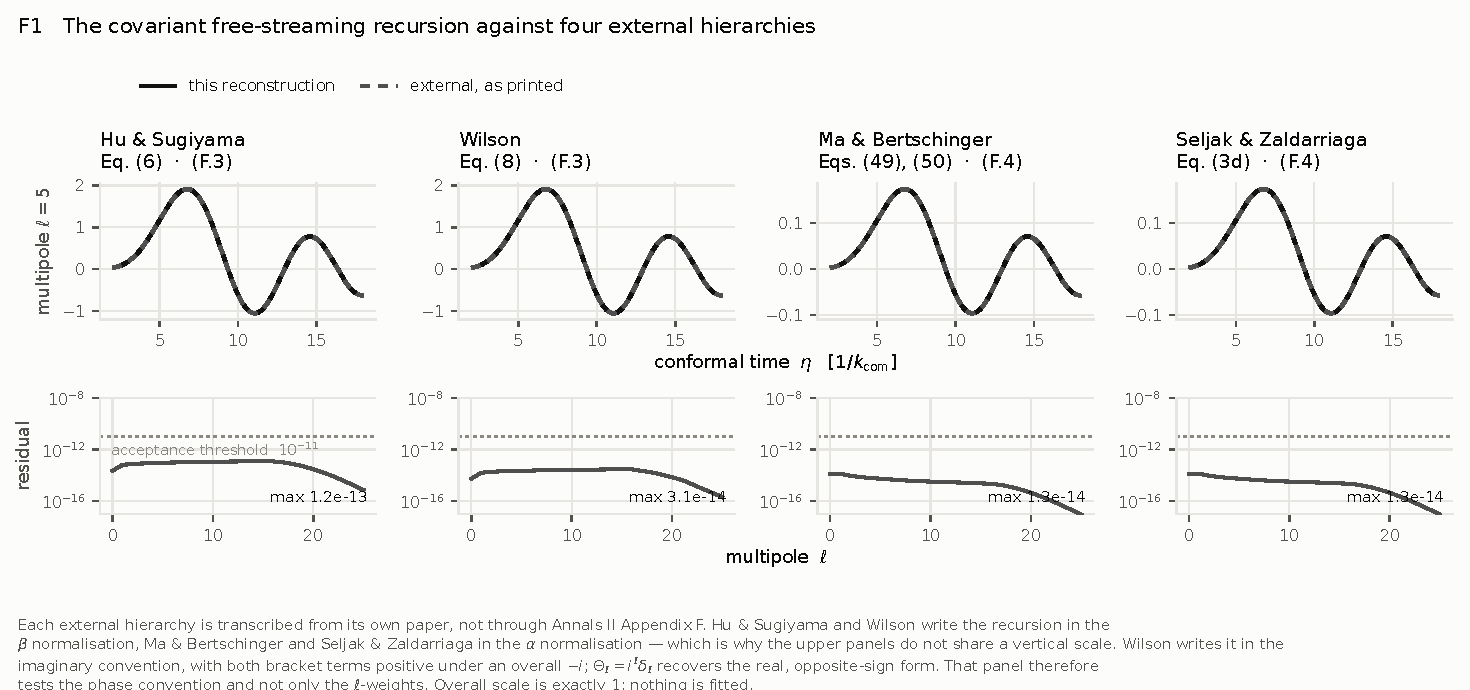
\includegraphics[width=\textwidth]{figures/f1-appendix-f-v1.0.0.pdf}
\caption[The covariant free-streaming recursion against four external hierarchies]{\textbf{F1 --- The covariant free-streaming recursion against four external hierarchies.} The covariant free-streaming recursion of \emph{Annals~II} Appendix~F, integrated from a unit monopole, against four external treatments of the same hierarchy. Each is transcribed from its own paper, never through Appendix~F. \textbf{Upper panels, context:} the reconstruction and the external form at $\ell=5$; they coincide. The panels do \emph{not} share a vertical scale, because two normalisations are on display. \textbf{Lower panels, the claim:} $\max_\eta|\mathrm{external}-\mathrm{reconstruction}|$ against $\ell$, with the acceptance threshold marked. Hu \& Sugiyama write the recursion in the $\beta$ normalisation and Ma \& Bertschinger and Seljak \& Zaldarriaga in the $\alpha$ normalisation, which is why Appendix~F prints both (F.3) and (F.4); a basis phase leaking into the couplings would break at least one match. Overall scale is exactly $1.000000000$ --- nothing is fitted. Four panels from five sources: Wilson \& Silk (1981) is the earliest, but at $K=0$ it is Wilson (1983) Eq.~(8) exactly, so it is credited rather than drawn.\\[2pt]\footnotesize\emph{Evidence category:} cross-check. \emph{Generated by} \texttt{scripts/figure\_f1\_appendix\_f.py}. \emph{Standalone caption:} \texttt{captions/F1-appendix-f.md}.}
\label{fig:f1}
\end{figure}

\begin{figure}[p]
\centering
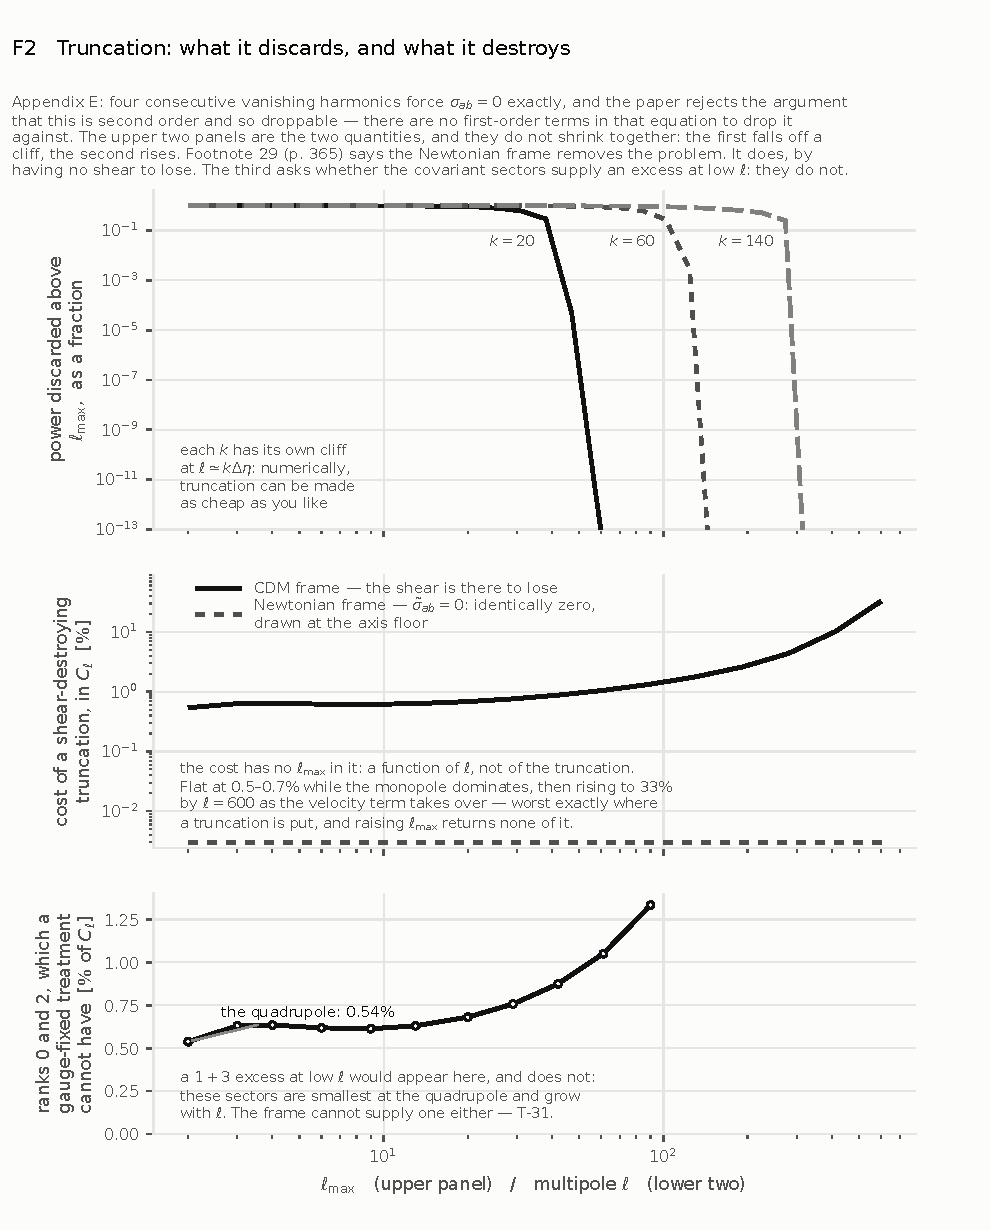
\includegraphics[width=0.95\textwidth]{figures/f2-truncation-v1.2.0.pdf}
\caption[What a truncation discards, and what it destroys]{\textbf{F2 --- What a truncation discards, and what it destroys.} Appendix~E of \emph{Annals~II} proves that four consecutive vanishing harmonics force $\sigma_{ab}=0$ exactly. This figure makes that quantitative in both frames, and the two panels answer two different questions that a single ``truncation error'' would blur.}
\label{fig:f2}
\end{figure}

\begin{figure}[p]
\ContinuedFloat
\captionsetup{font=footnotesize}
\caption[]{ \textbf{What a truncation \emph{discards}} falls off a per-$k$ cliff at $\ell\simeq k\,\Delta\eta$: above the cliff there is nothing left to keep, and the tail above $\ell=600$ is identically zero at every probe mode. \textbf{What it \emph{destroys}} has no $\ell_{\max}$ in it at all. Setting $\sigma_{ab}\to0$ costs $0.54$--$0.68\%$ out to $\ell\simeq20$, rises monotonically above $\ell=20$, and reaches $32.6\%$ by $\ell=600$ \textbf{[pre-T-57 values; this figure is superseded --- see the dagger]} --- a cost that grows with the multipole rather than being bounded by it, which is why a truncation argument cannot retire the shear.\\[2pt] \textbf{Footnote~29 (p.~365) is checked and upheld.} In the Newtonian frame the cost is \emph{identically zero}, median and maximum alike, because that frame has no shear to lose --- which is the content of the footnote's claim that the Newtonian specialisation removes the truncation problem. The script raises rather than draws if the Newtonian rank-0/2 sectors are ever non-empty, so the claim is a gate and not a caption.\\[2pt] \textbf{The third panel is the one that reports a negative result.} The rank-0/2 share is flat at the quadrupole ($0.54\%$) and rises only with $\ell$: a $1+3$ excess at low $\ell$ would appear here, and does not. That question is parked as \textbf{Q5}, and this panel is what parks it honestly.\\[2pt]$^{\dagger}$\,\emph{Superseded by finding} \textbf{T-57}\emph{; see} \texttt{provenance/BUNDLE-DEFECTS-v1.md}. \textbf{Its $k$ grid runs to 1900, not 420} --- finding \textbf{T-32}, where every v1.2.0 figure had been drawn on a grid stopping at the peak of the shear integrand. At $k_{\max}=1900$ against $k_D=754.6$ the damping envelope is $1.8\times10^{-3}$, and dropping the grid's top decile moves the cost by $3.4\times10^{-9}$. The lesson recorded there is the rule here: vary the limit and the resolution separately, because one grid number conflates them.\\[2pt]\footnotesize\emph{Evidence category:} cross-check. \emph{Generated by} \texttt{scripts/figure\_f2\_truncation.py}. \emph{Line-of-sight weight:} $\mathcal V$, the setting \texttt{line\_of\_sight\_weight}=\texttt{printed} selects. \textbf{The weight is a released knob and its two settings differ by the Sachs--Wolfe plateau and the late-time contribution}, so a figure that does not name it cannot be read; this artefact is not fingerprinted against its generator and predates the setting it now carries. \emph{Standalone caption:} \texttt{captions/F2-truncation.md}.}
\end{figure}

\begin{figure}[p]
\centering
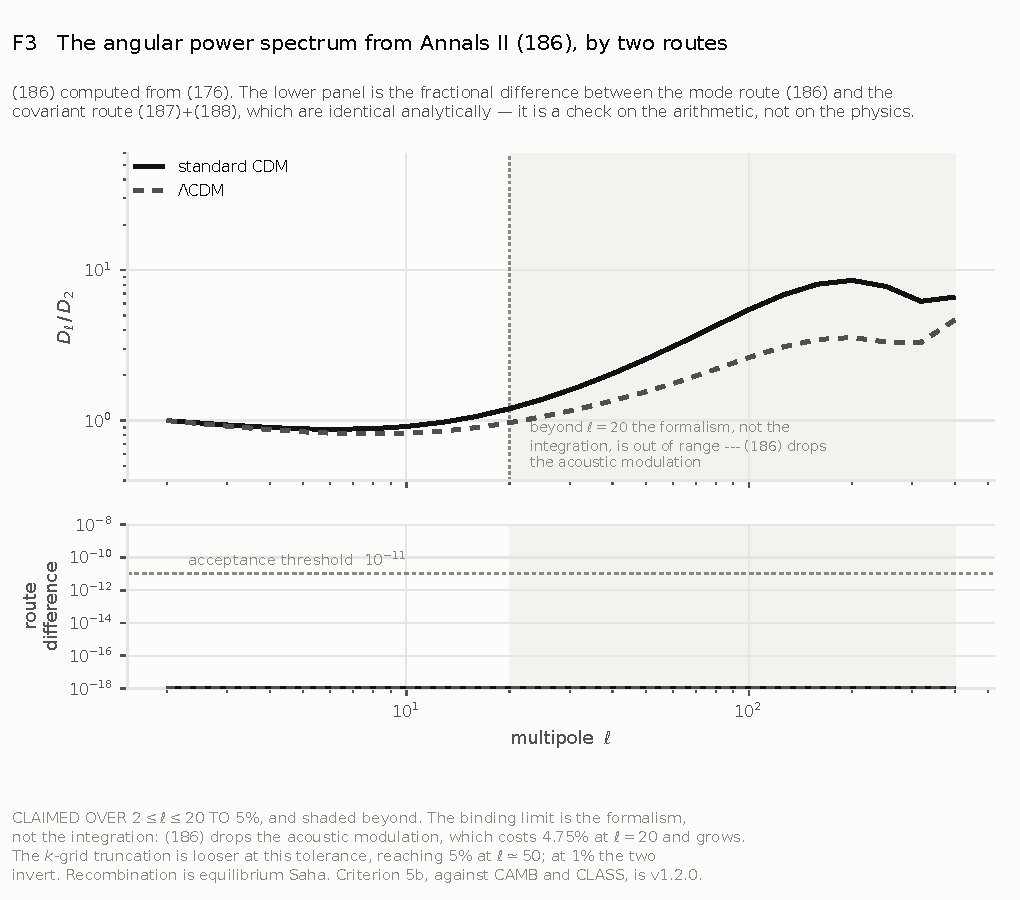
\includegraphics[width=\textwidth]{figures/f3-angular-spectrum-v1.0.0.pdf}
\caption[The angular power spectrum from Annals II (186), by two routes]{\textbf{F3 --- The angular power spectrum from Annals II (186), by two routes.} Eq.~(186) computed from Eq.~(176), for the standard-CDM model of \S8.3.2 and for $\Lambda$CDM, which \emph{Annals~II} does not treat. \textbf{Upper panel:} $D_\ell=\ell(\ell+1)C_\ell/2\pi$, each normalised to its own $\ell=2$ value, so that the comparison is of \emph{shape} and not of an amplitude neither model fixes here. \textbf{Lower panel:} the fractional difference between the mode route of (186) and the covariant route of (187) with (188). Those two are identical analytically, so the panel is a check on the arithmetic and not on the physics --- and it is worth having, because it caught a factor of four in this bundle's own harmonic weights before any figure was drawn. It sits at $10^{-16}$, five orders below the $10^{-11}$ acceptance threshold.\\[2pt]\footnotesize\emph{Evidence category:} recovery. \emph{Generated by} \texttt{scripts/figure\_f3\_angular\_spectrum.py}. \emph{Line-of-sight weight:} $\mathcal V$, the setting \texttt{Weighting.ANNALS\_II} selects. \textbf{The weight is a released knob and its two settings differ by the Sachs--Wolfe plateau and the late-time contribution}, so a figure that does not name it cannot be read; this artefact is not fingerprinted against its generator and predates the setting it now carries. \emph{Standalone caption:} \texttt{captions/F3-angular-spectrum.md}.}
\label{fig:f3}
\end{figure}

\begin{figure}[p]
\centering
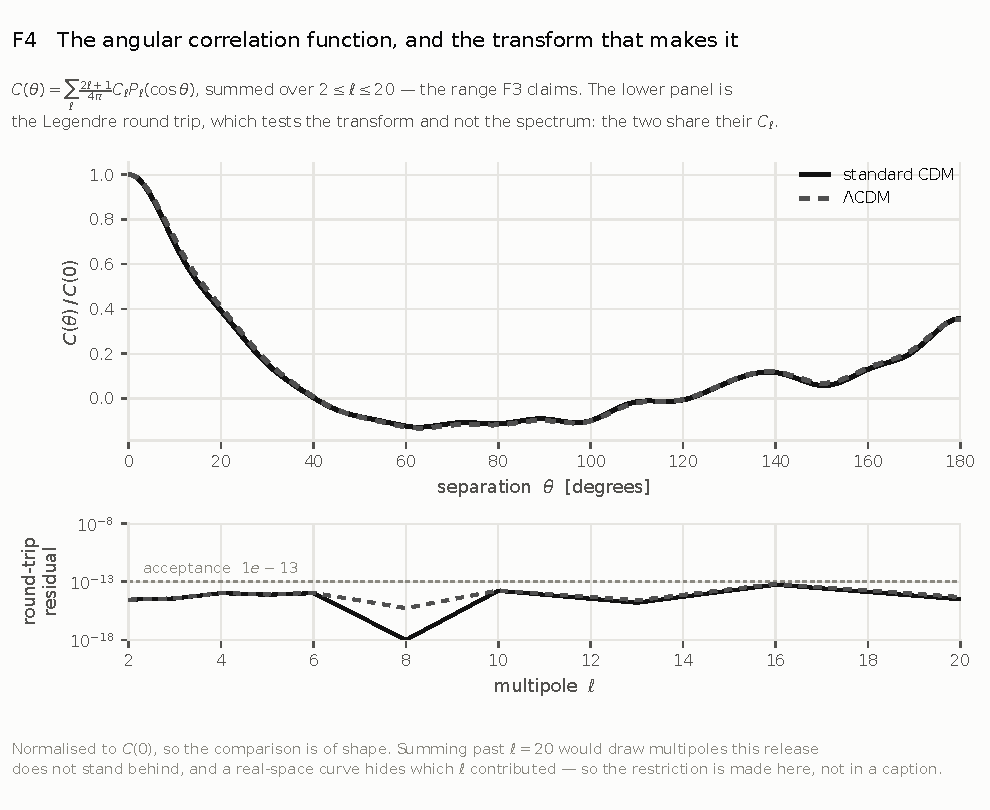
\includegraphics[width=\textwidth]{figures/f4-correlation-v1.0.0.pdf}
\caption[The angular correlation function, and the transform that makes it]{\textbf{F4 --- The angular correlation function, and the transform that makes it.} $C(\theta)=\sum_\ell\frac{2\ell+1}{4\pi}C_\ell P_\ell(\cos\theta)$, the real-space view of Figure~3: the same content read as a correlation between two directions separated by $\theta$ rather than as power at a multipole. \textbf{Upper panel:} $C(\theta)/C(0)$ for standard CDM and $\Lambda$CDM, summed over $2\le\ell\le20$ --- the range Figure~3 claims, bounded by (186) dropping the acoustic modulation. Summing further would draw multipoles this release does not stand behind, and a real-space curve hides which $\ell$ contributed, so the restriction is made in the transform rather than in this caption. \textbf{Lower panel:} the Legendre round trip $C_\ell\to C(\theta)\to C_\ell$, at $4\times10^{-14}$ and $7\times10^{-14}$ against an acceptance of $10^{-13}$. It tests the transform and \emph{not} the spectrum --- the two share their $C_\ell$ --- which is the same caution Figure~3's residual panel carries and for the same reason.\\[2pt]\footnotesize\emph{Evidence category:} acceptance. \emph{Generated by} \texttt{scripts/figure\_f4\_correlation.py}. \emph{Standalone caption:} \texttt{captions/F4-correlation.md}.}
\label{fig:f4}
\end{figure}

\begin{figure}[p]
\centering
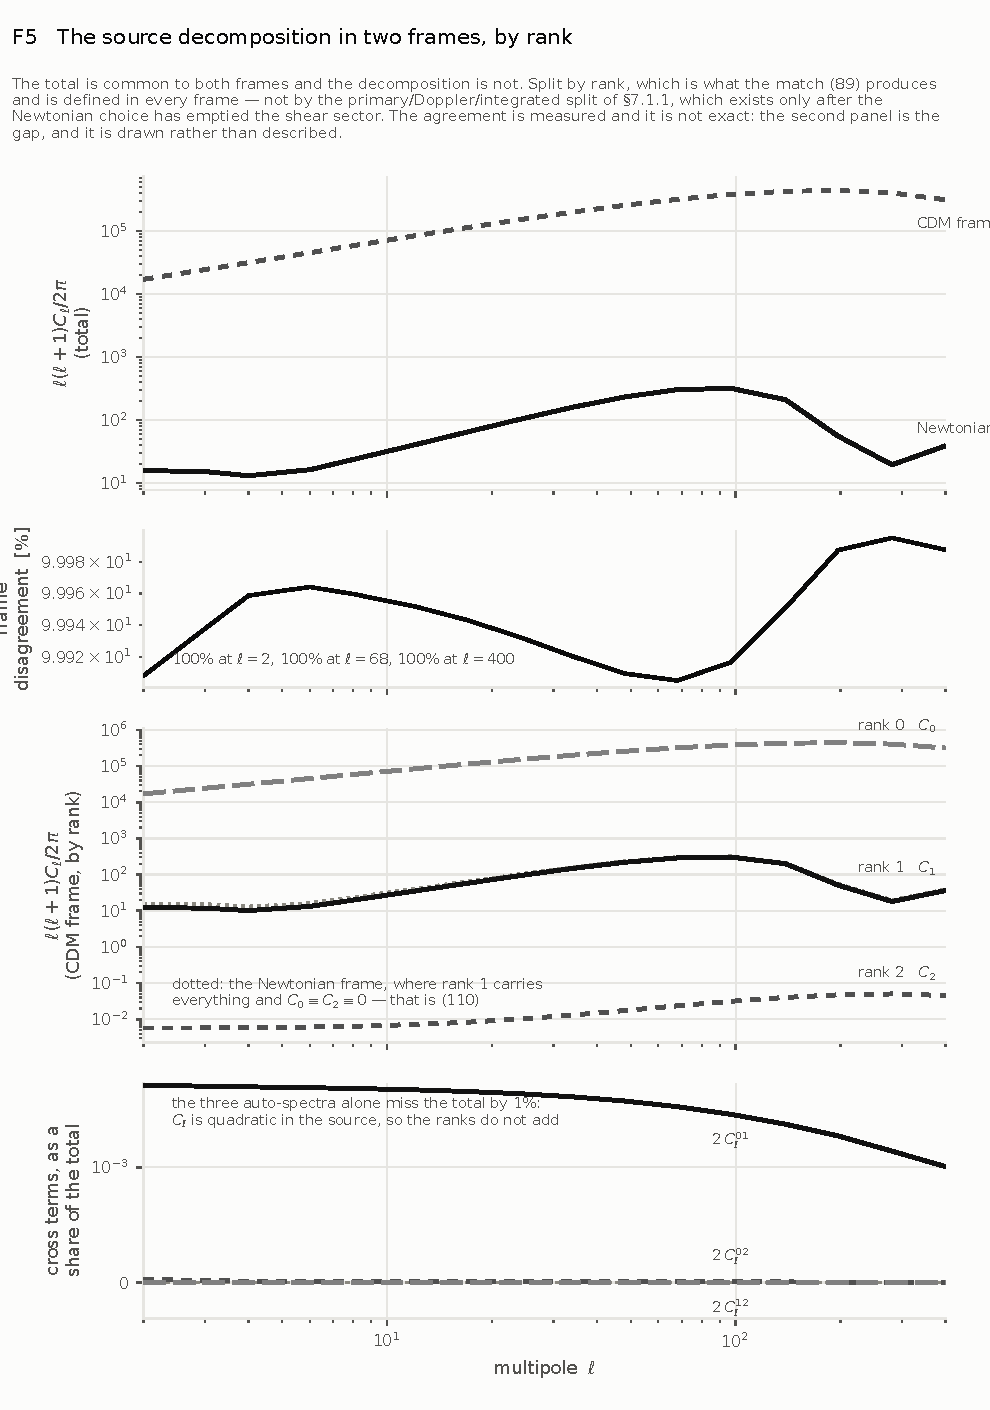
\includegraphics[width=0.82\textwidth]{figures/f5-sources-v1.2.0.pdf}
\caption[The source decomposition, by rank, in two frames]{\textbf{F5 --- The source decomposition, by rank, in two frames.} The integral solution~(102) carries three coefficients $C_0$, $C_1$, $C_2$ --- one per PSTF rank --- and this figure draws them, in the Newtonian frame and in the CDM frame, against $\ell$.}
\label{fig:f5}
\end{figure}

\begin{figure}[p]
\ContinuedFloat
\captionsetup{font=footnotesize}
\caption[]{ \textbf{Drawn in ranks, not in the Newtonian three-way split of \S7.1.1.} That was the PI's call, 2026-10-14, and it is a scientific choice rather than a presentational one: the primary/Doppler/integrated split is \emph{defined only in the frame it is written in}, while the rank decomposition is what~(89) produces and is defined in every frame. A figure comparing two frames must be drawn in a decomposition both of them have.\\[2pt] \textbf{The ranks sum to the total}, to $0$ exactly in the Newtonian frame and $4.1\times10^{-16}$ in the CDM frame --- which is the check that the decomposition is a decomposition and not three curves that happen to be near the answer. At the $C_\ell$ level the autos and twice the crosses reproduce $C_\ell$ to $4.7\times10^{-16}$ while the autos \emph{alone} are off by $0.10$: $C_\ell$ is quadratic in the transfer, so the cross terms are not a correction to be neglected but half the statement.\\[2pt] \textbf{The frame disagreement is the result, and it is its own panel.} The two frames' $C_\ell$ differ by a median of $15\%$ over $2\le\ell\le400$, worst $49\%$ \textbf{[pre-T-57/T-59 values; this figure is superseded --- see the dagger]}. That is not a defect: $C_\ell$ as computed here is built from frame-dependent pieces, and the invariance statement~(102) satisfies is about the \emph{total} at fixed $k$, which diagnostic~D6 measures separately. The median moved from $11\%$ to $15\%$ when finding \textbf{T-37} wired the transfer function, which is the kind of movement a figure should report rather than absorb.\\[2pt]$^{\dagger}$\,\emph{Superseded by findings} \textbf{T-57}\emph{,} \textbf{T-59}\emph{; see} \texttt{provenance/BUNDLE-DEFECTS-v1.md}.\\[2pt]\footnotesize\emph{Evidence category:} cross-check. \emph{Generated by} \texttt{scripts/figure\_f5\_sources.py}. \emph{Line-of-sight weight:} $\mathcal V$, the setting \texttt{line\_of\_sight\_weight}=\texttt{printed} selects. \textbf{The weight is a released knob and its two settings differ by the Sachs--Wolfe plateau and the late-time contribution}, so a figure that does not name it cannot be read; this artefact is not fingerprinted against its generator and predates the setting it now carries. \emph{Standalone caption:} \texttt{captions/F5-sources.md}.}
\end{figure}

\begin{figure}[p]
\centering
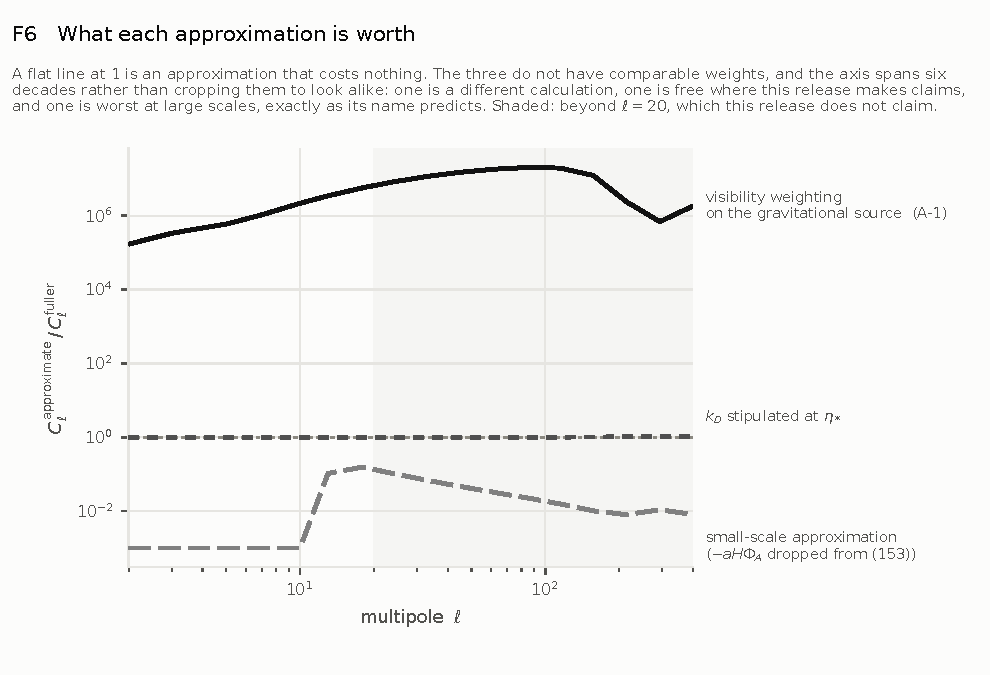
\includegraphics[width=\textwidth]{figures/f6-approximations-v1.1.0.pdf}
\caption[What each approximation is worth]{\textbf{F6 --- What each approximation is worth.} Each series is $C_\ell^{\mathrm{approximate}}/C_\ell^{\mathrm{fuller}}$ for standard CDM, so the panel is scale-free and a flat line at unity is an approximation that costs nothing. \emph{Annals~II} makes three narrowing choices which this bundle reproduces rather than corrects, because reproducing a paper means reproducing its approximations (decision~S15); they are recorded as \textbf{A-n} in \texttt{provenance/SOURCE-APPROXIMATIONS-v1.md}, deliberately apart from the defects recorded as \textbf{B-n}. This is the one place their cost is a number rather than an adjective.\\[2pt] \textbf{The three do not have comparable weights, and that is the result}, so the axis spans six decades rather than cropping them to look alike. The visibility weighting on the gravitational source (A-1) runs to $10^4$--$10^6$: it is a \emph{different calculation}, not a perturbation of one, which is why \texttt{Weighting} has no default. Stipulating $k_D$ at last scattering costs under $0.1\%$ across the claimed range and about $5\%$ by $\ell=400$ --- it \textbf{vindicates the release}, which takes the cheap choice where it makes claims. The small-scale approximation, dropping $-aH\Phi_A$ from~(153) and so producing the printed oscillator~(154), departs from unity most at \emph{large} scales, which is what its name predicts. \\[2pt] \textbf{A correction kept because it nearly became this figure.} The $k_D$ series was first computed with $k_D(\eta)$ along the whole ray. After last scattering $\kappa'\to0$, so $1/\kappa'$ in (dif-damp) diverges and $k_D$ collapses, damping every integrated source to nothing --- a plasma formula evaluated in a universe that no longer has a plasma. That version reported the release's choice as costing a factor of nine at $\ell=2$; the factor was the artefact. Clamped to $k_D(\min(\eta,\eta_*))$ the comparison is a real one. Shaded: beyond $\ell=20$, which this release does not claim.\\[2pt]\footnotesize\emph{Evidence category:} diagnostic. \emph{Generated by} \texttt{scripts/figure\_f6\_approximations.py}. \emph{Standalone caption:} \texttt{captions/F6-approximations.md}.}
\label{fig:f6}
\end{figure}

\begin{figure}[p]
\centering
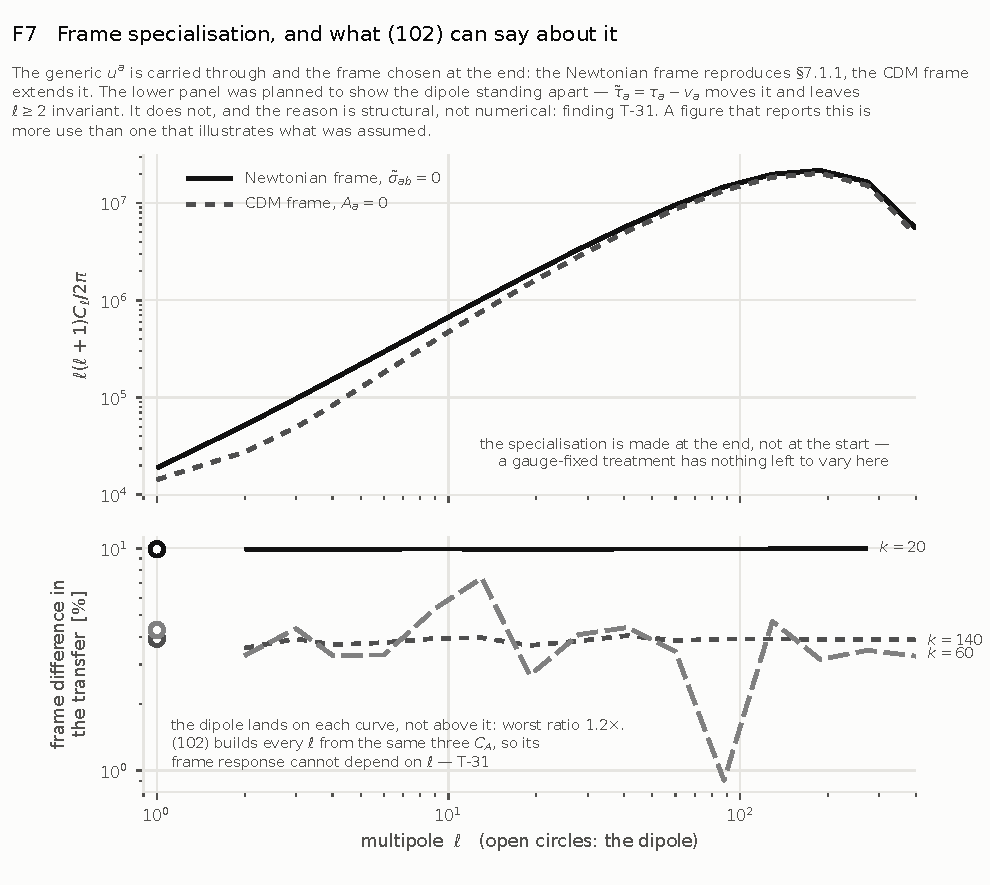
\includegraphics[width=\textwidth]{figures/f7-frames-v1.2.0.pdf}
\caption[Frame specialisation, and a planned claim that was false]{\textbf{F7 --- Frame specialisation, and a planned claim that was false.} \textbf{This figure reports that its own planned claim is false, and that is why it is here.} It was designed to show the dipole standing an order of magnitude apart from the higher multipoles under a change of frame --- the dipole being the one multipole a boost moves at first order. It does not. The dipole lands on each curve instead: worst ratio $1.25\times$ over the probe set, and $1.00\times$ at $k=20$.\\[2pt] \textbf{The reason is structural and is finding T-31.} Equation~(102) builds \emph{every} $\ell$ from the same three coefficients $C_A$, so a frame change that moves $C_1$ moves every multipole built on it in the same proportion. A frame response that depended on $\ell$ would contradict the equation's own form, and \texttt{test\_102\_cannot\_make\_its\_frame\_response\_depend\_on\_the\_multipole} asserts that it does not. The spread \emph{over} $\ell$ does grow with $k$ --- $1.01$, $1.14$, $8.14$ at $k=20$, $60$, $140$ --- but that is the transfer function's $k$ dependence, not the frame's $\ell$ dependence.\\[2pt] \textbf{A figure that had been drawn to its plan would have been drawn wrong.} The plan is kept in \texttt{captions/FIGURE-PLAN-v1.0.0.md} and the outcome is kept here, because a reproduction bundle whose figures only ever confirm their captions is not measuring anything.\\[2pt] \textbf{Its environment is built for the $k$ grid, not for the probe modes} --- finding \textbf{T-34}, where this figure sized its $\eta$ grid for $k=140$ and then integrated to $k=420$. \texttt{check\_k} now raises rather than interpolating past what the grid resolves.\\[2pt]\footnotesize\emph{Evidence category:} diagnostic. \emph{Generated by} \texttt{scripts/figure\_f7\_frames.py}. \emph{Line-of-sight weight:} $\mathcal V$, the setting \texttt{line\_of\_sight\_weight}=\texttt{printed} selects. \textbf{The weight is a released knob and its two settings differ by the Sachs--Wolfe plateau and the late-time contribution}, so a figure that does not name it cannot be read; this artefact is not fingerprinted against its generator and predates the setting it now carries. \emph{Standalone caption:} \texttt{captions/F7-frames.md}.}
\label{fig:f7}
\end{figure}

\begin{figure}[p]
\centering
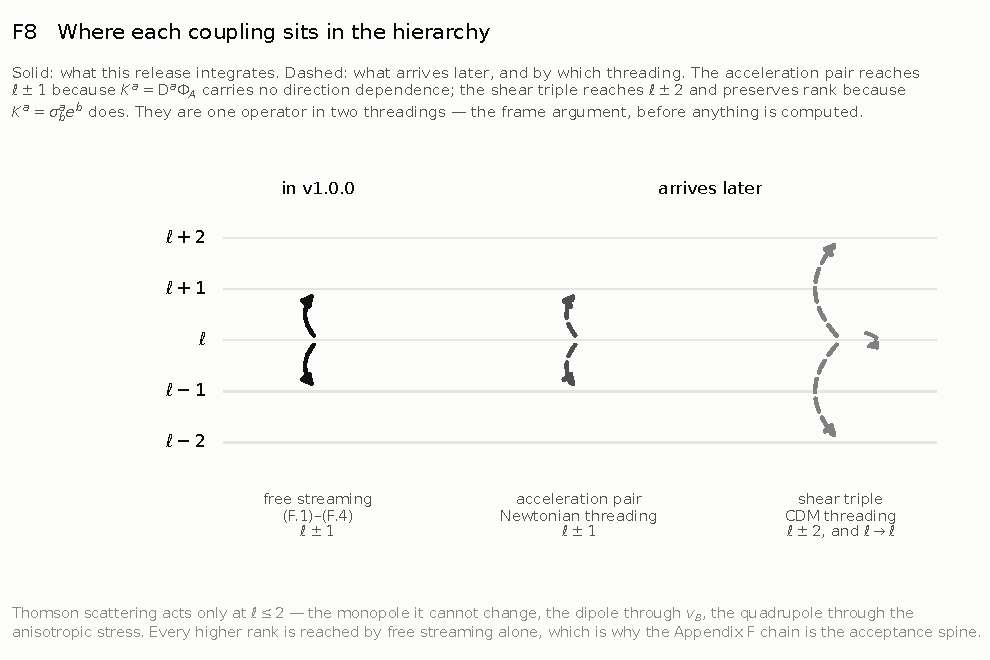
\includegraphics[width=\textwidth]{figures/f8-schematic-v1.1.0.pdf}
\caption[Where each coupling sits in the hierarchy]{\textbf{F8 --- Where each coupling sits in the hierarchy.} The one released figure that computes nothing: a statement about the \emph{structure} of the exact divergence hierarchy, read off the equations rather than measured. It is generated by a script like every other figure, so that the manifest covers it --- a hand-drawn diagram is the one artefact that can drift without any gate noticing.\\[2pt] \textbf{Solid:} what this release integrates. Free streaming, (F.1)--(F.4), couples rank $\ell$ to $\ell\pm1$ and to nothing else, which is the whole of v1.0.0's hierarchy and the reason the Appendix~F chain is the acceptance spine. \textbf{Dashed:} what arrives later, and by which frame. The acceleration pair reaches $\ell\pm1$ because $K^a=\mathrm{D}^a\Phi_A$ carries no direction dependence of its own; the shear triple reaches $\ell\pm2$ \emph{and} preserves rank because $K^a=\sigma^a{}_be^b$ does. The rank-preserving coupling exists only when $K^a$ depends on direction, and is the single structural difference between the two frames.\\[2pt] Both are the same operator $K_\perp^a\partial/\partial e^a$, and the number of ranks each reaches is fixed by that one property. \textbf{That is the whole content of the frame argument, visible before any of it is computed.} Decision S9 is drawn as well as asserted: every coupling in the solid half is a ratio of linear polynomials and tends to a constant, so an $O(\ell)$ coupling wired in early would fail \texttt{tests/test\_appendix\_f\_chain.py} at large $\ell$.\\[2pt]\footnotesize\emph{Evidence category:} schematic. \emph{Generated by} \texttt{scripts/figure\_f8\_schematic.py}. \emph{Standalone caption:} \texttt{captions/F8-schematic.md}.}
\label{fig:f8}
\end{figure}

\begin{figure}[p]
\centering
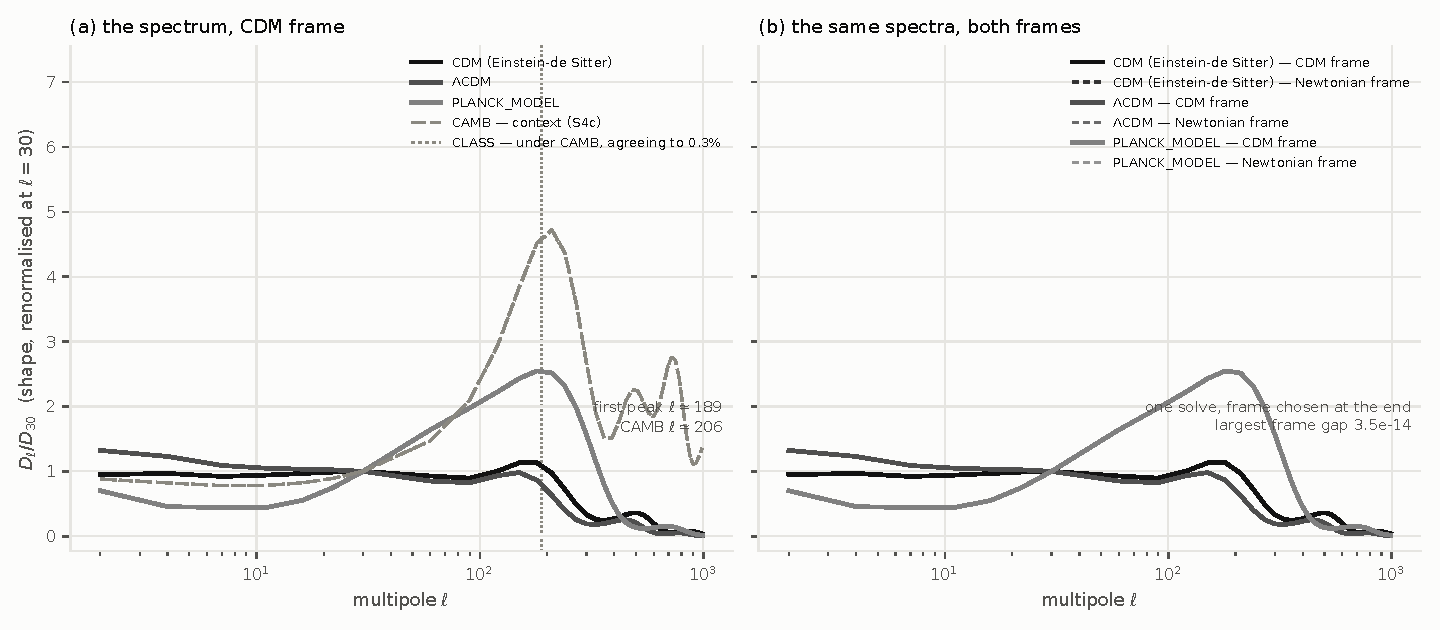
\includegraphics[width=\textwidth]{figures/f9-acoustic-spectrum-v1.2.0.pdf}
\caption[The angular spectrum with the acoustic peaks, in both frames]{\textbf{F9 --- The angular spectrum with the acoustic peaks, in both frames.} \textbf{The angular power spectrum for the three backgrounds this bundle ships} --- CDM (Einstein--de~Sitter), $\Lambda$CDM and the stamped Planck~2018 set --- as shape, $D_\ell$ renormalised at $\ell=30$.\\[2pt] \textbf{The line of sight is the supplement's eq.~\eqref{eq:assembly-invariant}}, built from the coefficients with Paper~1's source signs: the Sachs--Wolfe and Doppler terms where photons scatter, the integrated Sachs--Wolfe term along the path, each invariant under a change of frame, and no coefficient that holds the scattering rate differentiated.\\[2pt] \textbf{Panel (a) --- the spectrum, CDM frame.} The odd acoustic peaks are present, $2\ell_A$ apart; the first is at $\ell\simeq189$ on Planck ($0.71\,\ell_A$), $144$ on $\Lambda$CDM and $165$ on Einstein--de~Sitter. The even peaks are absent, as an oscillator driven by a constant potential and loaded with baryons predicts: the radiation-era driving that sets the peak heights is not yet in the source (\textbf{A-3}). Below $\ell\sim30$ the \texttt{PLANCK\_MODEL} curve, its dip near $\ell=5$ included, carries the incomplete radiation era of approximation \textbf{A-3}: the potential decays through equality while the oscillator starts from the matter-era adiabatic condition. It is not a prediction of v1.3.0. CAMB and CLASS are context, not a target (decision~\textbf{S4c}).\\[2pt] \textbf{Panel (b) --- both frames, from one solve.} The Newtonian and CDM spectra coincide to $3.5\times10^{-14}$ at every multipole: a first-order change of frame moves only the dipole, and here it moves nothing at $\ell\ge2$.\\[2pt]\footnotesize\emph{Evidence category:} acceptance. \emph{Generated by} \texttt{scripts/figure\_f9\_acoustic\_spectrum.py}. \emph{Standalone caption:} \texttt{captions/F9-acoustic-spectrum.md}.}
\label{fig:f9}
\end{figure}

\begin{figure}[p]
\centering
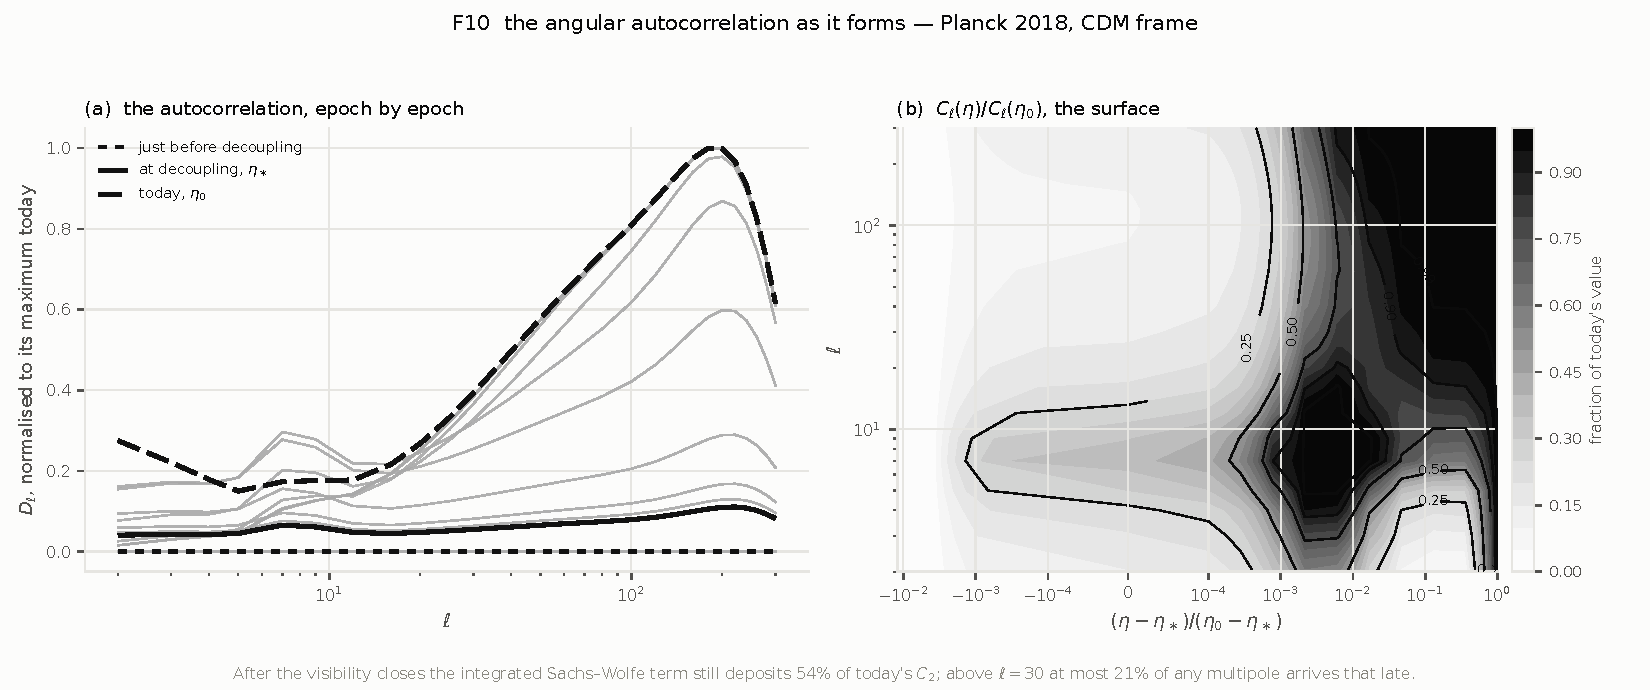
\includegraphics[width=\textwidth]{figures/f10-formation-surface-v1.3.0.pdf}
\caption[The angular autocorrelation as it forms: $C_\ell(\eta)$]{\textbf{F10 --- The angular autocorrelation as it forms: $C_\ell(\eta)$.} \textbf{The angular autocorrelation at a sequence of conformal times, and the surface it sweeps.} Planck~2018, CDM frame, 25 multipoles from $\ell=2$ to $\ell=300$, fourteen epochs from the start of recombination to today. The line of sight is eq.~\eqref{eq:assembly-invariant} with Paper~1's source signs, each slot accumulated to each epoch; the $\eta_0$ column is the full integral to $1.0\times10^{-13}$.\\[2pt] \textbf{(a)} $D_\ell$ against $\ell$, epoch by epoch, normalised once by the maximum of today's curve. \textbf{(b)} $C_\ell(\eta)/C_\ell(\eta_0)$ over the $(\ell,\eta)$ plane.\\[2pt] \textbf{What it shows.} Above $\ell\simeq30$ the spectrum is laid down while photons scatter, with $5$--$21\%$ of each multipole arriving afterwards from the integrated Sachs--Wolfe term as the potentials decay. At $\ell=2$--$4$ the late integrated Sachs--Wolfe term deposits $22$--$54\%$ of today's $C_\ell$, and at $\ell=5$--$12$ it cancels part of what recombination laid down. Every earlier version of this figure showed no late power at all; the assembly that replaced (102) restores it.\\[2pt]\footnotesize\emph{Evidence category:} diagnostic. \emph{Generated by} \texttt{scripts/figure\_f10\_formation\_surface.py}. \emph{Standalone caption:} \texttt{captions/F10-formation-surface.md}.}
\label{fig:f10}
\end{figure}

% === END source expansion: supplementary-materials/figures-v1.3.0.tex ===


\clearpage
\section{Release progression}
The release sequence is governed by the \emph{physics}, as specified in
the repository README. Two forms of testing must be distinguished. First, the v1.0.0 work established a
reproducible mathematical and computational verification basis for
the derivations and claims used by Paper~1, with the free-streaming,
normalisation, frame and Sachs--Wolfe checks providing specifically
identified evidence. A test of a source identity is evidence about
that identity; it is not a claim that the complete lensing and
aberration system has been implemented or independently certified.
Second, the subsequent v1.1.0--v1.5.0 physics releases successively
introduce physical terms into the software. Their acceptance tests
measure the \emph{implementation} and cannot replace verification
of the claims of Paper~1.

The release record is retained below, one physical milestone at a
time, separating what was \emph{achieved} from what was \emph{learned}.
The qualification of v1.0.0 is therefore precise: it established the
independent verification baseline and a first free-streaming
reconstruction; it did \emph{not} implement the full physics of
Paper~1. Paper~1's equations, especially its corrections of its
antecedents, remain the pivot for interpreting both classes of tests.
A later solver regression test becomes evidence for a Paper~1 claim
only when its derivation, assumptions and independence have also been
checked.
The additional claim-facing instruments in the current development branch
are inventoried separately in Table~\ref{tab:dev-claim-tests},
with the superseded C5 result specifically identified.

\subsection{Release sequence by physical objective}
\begin{itemize}\itemsep2pt
  \item v1.0.0 established a claim-facing verification baseline for
        Paper~1, including independent normalisation, phase, frame and
        free-streaming controls. Its tested implementation was the
        source-free reconstruction, not the complete nonlinear theory.
  \item v1.1.0 began the next physical implementation stage, asking
        \emph{what does the spectrum need that it does
        not have?} and answered: the visibility width.
  \item v1.2.0 asked \emph{is the antecedent's own algebra
        self-consistent when evaluated?} and answered yes, at $10^{-5}$,
        while finding that the question had been answered three times before
        without being measured.
  \item v1.3.0 asks \emph{where does the frame discrepancy come
        from?} --- and \S\ref{sec:frame-discrepancy} is the answer so far: not
        the source, not the by-parts bookkeeping, not the projection, but the
        slot-and-weight assignment of $C_1$. The question it has \emph{not}
        answered is whether repairing that assignment also recovers the
        acoustic peaks, which is a separate defect with a separate signature.
\end{itemize}


\paragraph{Claim-facing Python verification files.}
Table~\ref{tab:paper1-claim-python} identifies key test files present
at the \texttt{v1.0.0} repository tag whose \emph{mathematical content}
can be related to conventions or supporting claims in Paper~1.
This inventory is deliberately separate from test cases for the
software implementation. Each row states what was checked, not an
unrestricted claim of proof, and a mixture of symbolic assertions
and comparisons against bundle functions is identified as such.
The independent status of an individual assertion is determined by
what that assertion actually imports or derives, not by its
directory name or a passing test report. This is an extensible
ledger: additional claim-facing files from v1.1.0 or subsequent
releases must be added only with their exact Paper~1 reference,
scope, source revision and verification status.

\begin{table}[H]
\centering\footnotesize
\caption{\textbf{Python tests relevant to claims or conventions in Paper~1,
distinguished from solver implementation tests.} Files in this table
were checked at the stated repository tag. The last column
limits the claim supported; it does not rate the physical accuracy of
a spectrum. The machine-readable ledger records the exact GitHub
blob hashes.}
\label{tab:paper1-claim-python}
\begin{tabularx}{\linewidth}{@{}p{0.25\linewidth}p{0.31\linewidth}X@{}}
\toprule
\textbf{Python file and release} & \textbf{Paper~1 link and check} &
\textbf{Evidence boundary}\\
\midrule
\texttt{tests/}\newline\texttt{test\_appendix\_f\_chain.py}\newline(v1.0.0)
& Table~III C4--C5: PSTF harmonic weights,
$\beta_\ell$ recurrence, reality and relative sign;
free-streaming against four antecedent forms
& Exact symbolic/rational checks and external-form
comparisons; some assertions also compare against
bundle harmonics. This does not verify Paper~1's
nonlinear lensing operator.\\[3pt]
\texttt{tests/}\newline\texttt{test\_frames.py}\newline(v1.0.0)
& Paper~1 Eqs.~(8)--(10): frame transformation
and first-order kinematic relations
& Symbolic $Hv$ cancellation and negative controls;
tests import \texttt{functions/frames.py}. A
first-order frame identity is not the full
second-order, common-endpoint sky test.\\[3pt]
\texttt{tests/}\newline\texttt{test\_frames.py}\newline(v1.1.0 extension)
& Paper~1 Table~III C2.5 and Secs.~II~E, VI:
additional checks on the Weyl combination, the
geodesic-frame condition and the first-order dipole shift
& The later test revision adds exact-algebra assertions,
but uses the bundle's \texttt{functions/frames.py}.
These are claim-related controls, not an independent
nonlinear sky or spectrum certificate.\\[3pt]
\texttt{tests/}\newline\texttt{test\_angular.py}\newline(v1.0.0)
& Paper~1 Table~III C5.2--C5.3: harmonic
normalisation and the mode--covariant spectrum relation
& Exact-rational normalisation checks plus bundle
comparison; \emph{linear} $C_\ell$ algebra, not
Paper~1 Sec.~VII's quartic lensing-power cancellation.\\[3pt]
\texttt{tests/}\newline\texttt{test\_sachs\_wolfe.py}\newline(v1.0.0)
& Ordinary Sachs--Wolfe limit used as the linear
primary-sky input to Paper~1 Sec.~V
& Direct quadrature checks the antecedent's
printed Bessel relation; does not test the late
nonlinear aberration or curvature contribution.\\
\bottomrule
\end{tabularx}
\end{table}

\paragraph{Implementation acceptance tests are a separate inventory.}
For example, the v1.1.0 Peebles and frame-transformation
tests (\texttt{test\_peebles.py} and
\texttt{test\_frame\_transform.py}) check recombination
and implemented frame transformations.
They do not retroactively expand the independent Paper~1
v1.0.0 certificate. Likewise tests for
\texttt{coefficients.py}, the line-of-sight pipeline, and the
spectrum's morphology address the later \emph{physics
implementation}; they are not entered in
Table~\ref{tab:paper1-claim-python} merely because they pass.
New independent Paper~1 checks may be appended to this table in
v1.1.0 and later as their actual evidence is established.
The table is not an assertion that every major Paper~1
theorem has a completed standalone Python proof.
The original v1.0.0 tests and later extensions are recorded
at their actual Git tags; importing software-under-test
never becomes an independent derivation simply because
the test is mathematically phrased.

\subsection{v1.0.0 --- the reconstruction, and whether it is faithful}
Achieved. The free-streaming chain of Appendix~F reproduced against
\emph{four} external hierarchies --- Hu \& Sugiyama Eq.~(6), Wilson Eq.~(8),
Ma \& Bertschinger Eqs.~(49)/(50), Seljak \& Zaldarriaga Eq.~(3d) --- each read
from its own paper and integrated as printed, at residuals of
$10^{-13}$--$10^{-14}$ against a $10^{-11}$ threshold, in two normalisations
and two phase conventions. The almost-Friedmann--Lemaitre spectrum (186)
computed from (176) by the mode route and the covariant route, agreeing
exactly. The Sachs--Wolfe limit recovered at $0.26\%$ against a $5\%$
criterion. This shows that the reconstruction is faithful to the
antecedent's own equations, independently of any Boltzmann code, and that the
harmonic phase convention is fixed by the \emph{definition} of $Q_{A_\ell}$
rather than adopted.

Learned, and it set the pattern for everything after. A coarsened
$\eta$ grid returned a smooth, plausible spectrum that was $575\%$ wrong while
the two routes agreed to $10^{-16}$ --- finding T-3. Two
agreeing routes agree about what they share. That sentence is the single most
load-bearing lesson in this bundle; it produced \texttt{required\_n\_eta}, it is
why criterion~5b's gate states its shared inputs explicitly, and it is why the
grid register exists.

\subsection{v1.1.0 --- the recombination that makes peaks possible}
Achieved. Peebles' effective three-level atom replacing equilibrium
Saha, and made the default only after being checked standalone against the
standard ionisation history. Freeze-out at $2.15\times10^{-4}$ against a
standard $\sim2\times10^{-4}$; the visibility peak moves $z\simeq1300\to1107$
against a standard $1080$--$1100$, and the function \emph{widens by about
40\%}. The frame change made numerical rather than symbolic. This shows
that the width, not the position, is what the spectrum needs: the width sets
the Silk damping envelope, which is why the acoustic peaks could not be
attempted before this release.

Learned. \texttt{SAHA} was kept rather than deleted. A known-worse
alternative that \emph{must} change the answer is evidence; deleting it would
have left the improvement asserted rather than measured. The same principle
appears as the negative control in every criterion that claims one.

\subsection{v1.2.0 --- the spectrum with structure, and the audit of it}
Achieved. The full linear $C_\ell$: acoustic peaks, a Silk damping
tail, the complete source assembly, and the integral solution~(102) carried
with a generic $u^a$ and specialised back. Criterion~5b closed at
$9.5\times10^{-6}$ against a gate of $10^{-3}$. This shows that
\emph{Annals~II}'s two writings of its own integral solution --- (102)
specialised, and (177)--(179) assembled --- are the same calculation when
evaluated, which the paper recovers symbolically and which nobody had ever
computed.

Learned, three times over, and they are the same lesson in three
places. \emph{First}, the tolerance this criterion was written against could
only ever be failed: a slow-decoupling solution with no polarisation hierarchy
cannot meet two full Boltzmann codes, and a criterion that can only be failed
is not a criterion (S4c). \emph{Second}, the figure
$10^{-5}$ that had stood in the record for the two routes' agreement was never
measured --- it came from a fixed grid on which both routes were
\emph{un-converged in the same direction} (T-45). \emph{Third}, the
gate written to catch all of this printed \texttt{PASS} on a \texttt{nan},
because \texttt{nan >= gate} is \texttt{False} (T-44). A gate
is not tested by the run that passes it.

\subsection{v1.3.0 --- the structural audit, and the discrepancy localised}
Two halves, in the order decision~S37 fixed: the structural audit of
the code first, the acoustic modes second. The audit produced the generated
registers this supplement now rests on --- the grid register, which walks the
abstract syntax tree and \emph{fails} when the code holds a discretisation the
register does not name; the model table, derived from the \texttt{Background}
objects the code integrates rather than transcribed from a parameter sheet; and
the theory audit, generated from six self-contained instruments that import no
project code.

The acoustic half did not go as planned, and the record says so. It began as a
search for the missing peaks and became the localisation in
\S\ref{sec:frame-discrepancy}, because the frame discrepancy turned out to be
upstream of the peak question and to admit a cleaner instrument. Two
defects were separated that had been one symptom: the frame gap, now reduced
to a single site with both of its boundaries measured; and the peak positions,
which sit above their own $\ell_A$ on all three backgrounds, in both frames,
and which the acoustic scale does not explain --- the signs are opposite.

What v1.3.0 has not done. It has not repaired the assignment, it has
not recovered the peaks, and it has not bounded the envelope approximations
A-3, A-5 and the damping inputs, which are deferred to v1.4.0 precisely because
changing an envelope term mid-measurement moves the number being measured for
reasons unrelated to it.

What the arc did not do, and says so. No release has bounded the
accuracy of the \emph{source} as distinct from the consistency of its
assembly. The recombination grid moves the primary term by $1.2\%$ and both
routes of criterion~5b share it, so the criterion cannot see it. That is
recorded as a stated limit of v1.2.0 and derived immediately after the tag.

\paragraph{Planned end of the implementation sequence.}
The physics-facing objective of v1.5.0 is to bring the \emph{full
in-scope physics introduced in Paper~1} into the implementation:
the $O(\varepsilon^2\ell)$ kinematic couplings, their frame
relabelling and lensing/aberration interpretation, after v1.3.0
has closed the linear assembly and v1.4.0 has supplied the
radiation-era and tight-coupling ingredients. Every antecedent
relation must be used with the corrections and provenance
qualifications recorded in Paper~1 and this supplement. This is
the \emph{planned endpoint}, not a claim that v1.5.0 has been
implemented, that all components have been independently
certified, or that Paper~1 computes out-of-scope tensor amplitudes
or polarisation.

% The scattering-strength expansion. SELF-CONTAINED and movable: this
% line and tables/scattering-expansion-v1.3.0.tex are the whole of it,
% so relocating it to Paper 2 is a file move. Decision S42.

% === BEGIN exact v1.3.0 source expansion: supplementary-materials/appendix-scattering-expansion-v1.3.0.tex ===
% ---------------------------------------------------------------------------
% The scattering-strength expansion, re-derived.
%
% SELF-CONTAINED BY DESIGN. This file inputs one generated table and defines
% nothing; it can be moved into Paper 2 by moving two files, this and
% tables/scattering-expansion-v1.3.0.tex. Decision S42.
% ---------------------------------------------------------------------------
\section{The scattering-strength expansion, re-derived}
\label{sec:scattering-expansion}

\emph{Annals~II} Appendix~C writes the almost-Friedmann--Lema\^{\i}tre
integrated Boltzmann equation for Thomson scattering as
\begin{equation}
  \mathcal B+\dot\tau+e^a\mathrm D_a\tau \;\simeq\; t_c^{-1}\big[v^ae_a-\tau\big],
  \label{eq:ibe-thomson}
\end{equation}
inverts it, and approximates the result \emph{``systematically \dots in terms
of the smallness parameter $t_c$''} by the recursion
\begin{equation}
  \tau_{(n)} \;\simeq\; v^ae_a-t_c\Big[\mathcal B+\dot\tau_{(n-1)}
  +e^a\mathrm D_a\tau_{(n-1)}\Big],
  \label{eq:appc-recursion}
\end{equation}
printing $\tau_{(0)}$, $\tau_{(1)}$ and $\tau_{(2)}$. Section~5.5.3,
\emph{Expansion in Thompson Scattering Time}, states that the scheme carries
\emph{``terms up to $\mathcal O(t_c^3)$''}, so the ceiling is the antecedent's
and the printed orders stop one short of it.

\subsection{The recursion is geometric}

Write $\mathcal D\equiv\partial_t+e^a\mathrm D_a$ for the derivative along the
photon path --- which is exactly the pair of terms \eqref{eq:appc-recursion}
applies to $\tau_{(n-1)}$ --- and $V\equiv v^ae_a$. Then
\eqref{eq:ibe-thomson} reads $\tau=V-t_c(\mathcal B+\mathcal D\tau)$, so
\begin{equation}
  \big(1+t_c\mathcal D\big)\tau=V-t_c\mathcal B,
  \qquad
  \tau=\big(1+t_c\mathcal D\big)^{-1}\big(V-t_c\mathcal B\big),
  \label{eq:closed-operator}
\end{equation}
and expanding the inverse as a Neumann series in $(-t_c\mathcal D)$ gives a
closed form at every order:
\begin{equation}
  \boxed{\;\tau_{(n)}\;=\;V\;+\;\sum_{m=1}^{n}(-1)^m\,t_c^m
  \Big[\mathcal D^{m}V+\mathcal D^{m-1}\mathcal B\Big].\;}
  \label{eq:closed-form}
\end{equation}

This shows that Appendix~C's recursion is not an open-ended
approximation scheme but a geometric series with an explicit sum, and that
$\tau_{(1)}$ and $\tau_{(2)}$ as printed are its first two partial sums.
Equation~\eqref{eq:closed-form} is implemented in
\texttt{functions/spectra/scattering\_expansion.py} and checked against the
printed $\tau_{(1)}$ and $\tau_{(2)}$ term for term, with a deliberately
failing control, in \texttt{tests/test\_scattering\_expansion.py}. The closed
form was derived from \eqref{eq:appc-recursion} and \emph{then} compared with
the page, which is the only order in which the comparison carries information.

\paragraph{The closed form holds the scattering time fixed along the path, and
the antecedent's scheme is what fixes it.} The Neumann series of
$(1+t_c\mathcal D)^{-1}$ runs in powers of the \emph{operator} $t_c\mathcal D$,
and $(t_c\mathcal D)^2=t_c(\mathcal Dt_c)\mathcal D+t_c^2\mathcal D^2$.
Iterating \eqref{eq:appc-recursion} directly returns
$t_c(\mathcal Dt_c)\mathcal B$ and $t_c(\mathcal Dt_c)(\mathcal DV)$ at second
order; neither appears in \eqref{eq:closed-form}, which carries scalar powers
$t_c^m$ against operator powers $\mathcal D^m$. The term counts say whose
omission it is. \eqref{eq:closed-form} holds $2^m+2^{m-1}$ terms and
Appendix~C prints three at first order and six at second, which it could not do
if the $\mathcal Dt_c$ terms were carried. The reconstruction is faithful to
the page; the scheme on the page sets $\mathcal Dt_c=0$ without saying so.

\paragraph{At the peak of the visibility the dropped term is the size of the
term one order below it.} In conformal time $t_c=1/\kappa'$, so along the time
direction $\mathcal Dt_c=-\kappa''/\kappa'^2$. The visibility
$\mathcal V=\kappa'e^{-\kappa}$ is stationary where
$\mathcal V'=(\kappa''+\kappa'^2)e^{-\kappa}$ vanishes, and $e^{-\kappa}$ never
does, so the peak sits exactly at $\kappa''=-\kappa'^2$ --- measured to
$7.4\times10^{-15}$ in \texttt{tests/frame/c12\_sampling\_bound.py}. There
$\mathcal Dt_c=1$, and the dropped $t_c(\mathcal Dt_c)(\mathcal DV)$ is
$t_c\mathcal DV$, which is the retained first-order term. The second-order
remainder is the size of the first order at $\eta_\ast$, so the series is not
asymptotic at the one epoch it is applied to. Two parameters control it and
only one is small: $t_ck$ for the gradients, and $t_c\mathcal D\ln t_c$ for
the time derivative, which is unity at the peak whatever $k$ is.

\subsection{Two consequences the closed form makes immediate}

\paragraph{The term counts are not chosen.} $\mathcal D^m$ expands into a sum
over words in $\{\partial_t,\;e^a\mathrm D_a\}$, so the $t_c^m$ bracket of
\eqref{eq:closed-form} holds exactly $2^m+2^{m-1}$ terms. Appendix~C prints
three at first order and six at second; those are $2+1$ and $4+2$.
Table~\ref{tab:scattering-expansion} lists every term to
$\mathcal O(t_c^3)$, generated from the same module rather than transcribed.

\paragraph{Order $m$ sources multipoles up to $\ell=m+1$.} Each
$e^a\mathrm D_a$ carries one direction vector and $V=v^ae_a$ carries one
already, so a word with $g$ gradients seeded by $V$ has $g+1$ factors of
$e^a$; reduced by Appendix~C's own solid-angle identities, which lower the rank
two at a time, its highest PSTF part has rank $g+1$. At second order that
reaches rank three, in the single term
$e^ce^ae^b\mathrm D_c\mathrm D_av_b$.

Equivalently, and more usefully for the high-$\ell$ question: each gradient
contributes one power of $k$, so a term of rank $r$ carries $k^{\,r-1}$. The
expansion parameter is therefore $t_ck$ --- the ratio of the mean free path to
the wavelength --- and not $t_c$ alone. This shows that the
truncation is $\ell$-dependent by construction: a cut in rank is a cut in
$t_ck$, and the order at which the expansion may be stopped falls as $\ell$
rises.

\subsection{What this costs the oscillator}

The near-tight-coupling set of \S7.1 is introduced \emph{``rewritten to first
order''} and closes with $\tau^{A_\ell}\simeq0$ for all $\ell>2$. At first
order the expansion reaches rank two, so the closure costs nothing and the
antecedent is consistent. What the rank counting fixes is the price of
going further: second order reaches the octupole and
$\mathcal O(t_c^3)$ the hexadecapole, and the closure carried with (152) and
(153) reaches neither.

That is approximation~A-4 of
\texttt{provenance/SOURCE-APPROXIMATIONS-v1.md} stated as a rank rather than as
a dropped term. The term the oscillator derivation discards,
$-\tfrac25 t_c(1+R)^{-1}\mathrm D^b\mathrm D_{\langle a}u^m_{b\rangle}$, is
dropped because \emph{``the matter shear is already at least first order''} ---
a cross term of $\mathcal O(t_c\epsilon)$ between \S5.5.1's almost-Friedmann--Lema\^{\i}tre
ordering and \S5.5.3's scattering-time ordering. \emph{Annals~II}'s
Appendix~E, after Ellis--Treciokas--Matravers, states what the discarded
harmonics hold: if any four consecutive ones vanish exactly then
$\sigma_{ab}=0$ exactly. This shows that the truncation and the shear
are not independent --- the residual in the truncated harmonics is where the
shear lives, and a treatment that sets them to zero has set the shear to zero
with them.

\subsection{What appears at second order that does not appear at first}

Appendix~C's own solid-angle reduction gives the rank decomposition of the
source,
\begin{equation}
  \int_{4\pi}\!\mathrm d\Omega\;O^{A_\ell}\mathcal B\simeq
  \delta^\ell_0\Big[-\tfrac{4\pi}{3}\mathrm D_a\tau^a\Big]
  +\delta^\ell_1\Big[\tfrac{4\pi}{3}\big(\tfrac14\mathrm D^{a_1}\ln\rho_R+A^{a_1}\big)\Big]
  +\delta^\ell_2\Big[\tfrac{8\pi}{15}\sigma^{a_1a_2}\Big],
  \label{eq:b-ranks}
\end{equation}
so $\mathcal B$ carries the shear in its rank-two part. At first order
$-t_c\mathcal B$ therefore reproduces the quadrupole
$\tau_{ab}\simeq-\dot\kappa^{-1}[\sigma_{ab}+\mathrm D_{\langle a}v_{b\rangle}^B]$
of \S7.1, as it must.

At second order the closed form contributes $+t_c^2\,\mathcal D\mathcal B$, and
through \eqref{eq:b-ranks} that is $\dot\sigma_{ab}$ at rank two and
$e^c\mathrm D_c\sigma_{ab}$ at rank three. Appendix~G's
$\dot\sigma_{ab}+2H\sigma_{ab}+E_{ab}\approx0$ then gives
\begin{equation}
  \dot\sigma_{ab}=-2H\sigma_{ab}-E_{ab},
  \label{eq:sigma-dot}
\end{equation}
so the electric Weyl tensor enters the radiation quadrupole at second
order in the scattering time, and does not at first. This shows that
the second-order expansion is not merely a smaller correction of the same kind:
it introduces a gravitational tidal driving of the quadrupole that the
first-order treatment has no term for.

\paragraph{An open question, stated as a mechanism rather than a result.}
\emph{Annals~II} flags the regime itself, in a footnote to the sentence about
removing the radiation quadrupole: \emph{``If there are any anisotropic
contributions such as anisotropic scattering (in the matter frame) or large
shear (from gravitational waves) at that time this sort of approximation should
be considered with care --- such phenomena would break tight-coupling.''} For a
tensor mode both $\sigma^{(T)}_{ab}$ and $E^{(T)}_{ab}$ oscillate at the
gravitational-wave frequency, so \eqref{eq:sigma-dot} drives the second-order
quadrupole oscillatorily on a scale set by the wave and not by the sound
horizon. Whether that survives projection as a distinguishable \emph{ringing}
is open; it is recorded as question~Q10 rather than claimed, because
nothing here computes it.

\paragraph{What this expansion cannot produce.} \eqref{eq:appc-recursion} is
linear in $V$ and $\mathcal B$, so \eqref{eq:closed-form} yields terms
of order $t_c^m\epsilon$ and never $\epsilon^2$. Terms of
$\mathcal O(\varepsilon^2\ell)$ require the quadratic parts of the Boltzmann
equation that \S5.5.1's almost-Friedmann--Lema\^{\i}tre linearisation discards,
and are the subject of a later release rather than of this appendix. The
high-$\ell$ sensitivity established above is a separate statement and rests on
$t_ck$, not on $\epsilon^2$.

% v1.3.5 PRESENTATION COPY; scientific rows unchanged from scattering-expansion-v1.3.0.tex
% GENERATED by scripts/make_tables.py from config/implementation-register.toml.
% Do not edit by hand.

\begingroup
\footnotesize
\setlength{\tabcolsep}{4pt}
\renewcommand{\arraystretch}{1.25}
\setlength{\LTcapwidth}{115mm}
\captionsetup{justification=raggedright,singlelinecheck=false} % avoid stretched caption
\begin{longtable}{@{}p{22mm}p{8mm}p{65mm}p{12mm}@{}}
\caption{\emph{Annals~II} Appendix~C's scattering-strength expansion to $\mathcal O(t_c^3)$, generated from \texttt{functions/spectra/scattering\_expansion.py}. \textbf{Rank} is the highest PSTF multipole the term can source: one per $e^a\mathrm D_a$, plus one for $V=v^ae_a$. The closure (L0082) keeps $\ell\le2$.}\label{tab:scattering-expansion}\\
\toprule
\textbf{Order} & \textbf{} & \textbf{Term} & \textbf{Rank} \\
\midrule
\endfirsthead
\toprule
\textbf{Order} & \textbf{} & \textbf{Term} & \textbf{Rank} \\
\midrule
\endhead
\bottomrule
\endfoot
$t_c^{0}$ & $+$ & $v_a e^a$ & 1 \\
$t_c^{1}$ & $-$ & $\mathcal{B}$ & 0 \\
$t_c^{1}$ & $-$ & $\big(v_a e^a\big)^{\textstyle\cdot}$ & 1 \\
$t_c^{1}$ & $-$ & $e^c \mathrm{D}_c\big(v_a e^a\big)$ & 2 \\
$t_c^{2}$ & $+$ & $\big(\mathcal{B}\big)^{\textstyle\cdot}$ & 0 \\
$t_c^{2}$ & $+$ & $e^c \mathrm{D}_c\big(\mathcal{B}\big)$ & 1 \\
$t_c^{2}$ & $+$ & $\big(\big(v_a e^a\big)^{\textstyle\cdot}\big)^{\textstyle\cdot}$ & 1 \\
$t_c^{2}$ & $+$ & $e^c \mathrm{D}_c\big(\big(v_a e^a\big)^{\textstyle\cdot}\big)$ & 2 \\
$t_c^{2}$ & $+$ & $\big(e^c \mathrm{D}_c\big(v_a e^a\big)\big)^{\textstyle\cdot}$ & 2 \\
$t_c^{2}$ & $+$ & $e^c \mathrm{D}_c\big(e^c \mathrm{D}_c\big(v_a e^a\big)\big)$ & 3 \\
$t_c^{3}$ & $-$ & $\big(\big(\mathcal{B}\big)^{\textstyle\cdot}\big)^{\textstyle\cdot}$ & 0 \\
$t_c^{3}$ & $-$ & $e^c \mathrm{D}_c\big(\big(\mathcal{B}\big)^{\textstyle\cdot}\big)$ & 1 \\
$t_c^{3}$ & $-$ & $\big(e^c \mathrm{D}_c\big(\mathcal{B}\big)\big)^{\textstyle\cdot}$ & 1 \\
$t_c^{3}$ & $-$ & $e^c \mathrm{D}_c\big(e^c \mathrm{D}_c\big(\mathcal{B}\big)\big)$ & 2 \\
$t_c^{3}$ & $-$ & $\big(\big(\big(v_a e^a\big)^{\textstyle\cdot}\big)^{\textstyle\cdot}\big)^{\textstyle\cdot}$ & 1 \\
$t_c^{3}$ & $-$ & $e^c \mathrm{D}_c\big(\big(\big(v_a e^a\big)^{\textstyle\cdot}\big)^{\textstyle\cdot}\big)$ & 2 \\
$t_c^{3}$ & $-$ & $\big(e^c \mathrm{D}_c\big(\big(v_a e^a\big)^{\textstyle\cdot}\big)\big)^{\textstyle\cdot}$ & 2 \\
$t_c^{3}$ & $-$ & $e^c \mathrm{D}_c\big(e^c \mathrm{D}_c\big(\big(v_a e^a\big)^{\textstyle\cdot}\big)\big)$ & 3 \\
$t_c^{3}$ & $-$ & $\big(\big(e^c \mathrm{D}_c\big(v_a e^a\big)\big)^{\textstyle\cdot}\big)^{\textstyle\cdot}$ & 2 \\
$t_c^{3}$ & $-$ & $e^c \mathrm{D}_c\big(\big(e^c \mathrm{D}_c\big(v_a e^a\big)\big)^{\textstyle\cdot}\big)$ & 3 \\
$t_c^{3}$ & $-$ & $\big(e^c \mathrm{D}_c\big(e^c \mathrm{D}_c\big(v_a e^a\big)\big)\big)^{\textstyle\cdot}$ & 3 \\
$t_c^{3}$ & $-$ & $e^c \mathrm{D}_c\big(e^c \mathrm{D}_c\big(e^c \mathrm{D}_c\big(v_a e^a\big)\big)\big)$ & 4 \\
\end{longtable}
\endgroup


\paragraph{One transcription note.} The fifth term of Appendix~C's $t_c^2$
bracket is printed as $e^ce^d\mathrm D_c\dot v_b$, which leaves both $d$ and
$b$ free in a scalar. It is $e^ce^d\mathrm D_c\dot v_d$ --- the time derivative
taken first and the gradient outside --- forced independently by the four words
of $\mathcal D^2$, by the bracket's count of six with the other five
unambiguous, and by the two direction vectors having nothing else to contract
with. Recorded as B-15; no computed quantity depends on it.

% === END source expansion: supplementary-materials/appendix-scattering-expansion-v1.3.0.tex ===


% === BEGIN exact v1.3.0 source expansion: supplementary-materials/appendix-frame-division-v1.3.0.tex ===
% ---------------------------------------------------------------------------
% The CDM-frame division of the GDE99 integral solution, term by term.
%
% SELF-CONTAINED BY DESIGN. Inputs nothing, defines nothing, moves as one file.
%
% REVISED 2026-10-18 after a check by the Paper 1 stream. The first draft
% framed this as Paper 1's work-list item 3 on the strength of a sentence
% quoted in a stream note -- "The CDM-frame division has not been computed
% term by term" -- which appears in NO release of Paper 1. Paper 1 does
% compute its own CDM division term by term (Sec. VI A), and that division is
% a different object: the split of the O(eps^2 ell) source between the
% aberration operator and the section geometry. Paper 1 contains no C_0, no
% C_1, no C_2, no visibility and no line-of-sight integral solution at all.
% This appendix is about the GDE99 integral solution and is bundle territory.
% ---------------------------------------------------------------------------
\section{The CDM-frame division of the integral solution, term by term}
\label{sec:frame-division}

The integral solution (102) is derived for a general $u^a$ --- the antecedent
says so immediately after (90), \emph{``Note that these are CGI with respect to
$u^a$''} --- and then evaluated once, in the Newtonian frame. This appendix
carries it into the CDM frame instead, coefficient by coefficient, and finds
that the two frames do not agree. The failure is isolated to one coefficient at
one power of $k$.

What this shows is narrower than it looks, and the conventions
section exists because the first draft of this appendix did not have one.

\subsection{Conventions, stated}
\label{sec:frame-division-conventions}

Every relation below is in one convention and this subsection fixes it. The
need for it was raised by the Paper~1 stream, whose check could not reproduce
two of the four frame-table entries --- correctly, because the entries are in
the bundle's normalisation and the check was in Paper~1's.

\paragraph{Wavenumber.} The bundle carries $k\equiv k_{\rm com}$ throughout and
converts at the point of use, $k_{\rm phys}=k_{\rm com}/a$. Paper~1's C3.1
declares $k$ \emph{physical}. So a relation printed there as $X=k\,Y$ is
carried here as $aX=k_{\rm com}Y$, and the scale factor is the conversion, not
a transcription error.

\paragraph{The frame velocity.} $v^a$ is the relative velocity of the two
frames, $\tilde u^a\approx u^a+v^a$ with $v_au^a=0$, expanded as $v_a=v\,Q_a$.
So $v$ is a \emph{velocity amplitude}: it is the $v$ of the Euler equation
$v'+\mathcal Hv=-k\Phi_A$, which is the frame condition $\tilde A_a=0$, and it
is the $v$ of $\sigma=-k_{\rm phys}v$. It is not a velocity potential;
$v_a=\mathcal D_aV$ would put $k$ in the numerator.

\paragraph{The dipole.} The bundle carries the dipole in the \emph{covariant}
normalisation, $\tilde\tau_1\equiv\tilde v_B=v_B/k$ --- the normalisation (109)
needs in order to read $-\tilde C_1=(\delta\tilde T+\Phi_A)+\kappa'\tilde v_B$.
GDE99~(37), $\tilde\tau_a\approx\tau_a-v_a$, therefore reads
$\tilde\tau_1\to\tilde\tau_1-v/k$ \emph{here} and $\tau_1\to\tau_1-v$ in the
un-reduced normalisation. The two are the same statement. This is finding
T-27 in the bundle's record, where the un-reduced form was used by mistake
and the symptom was a first-order frame change 186 times the quantity it
corrects at $k=300$.

\paragraph{Consequently, two of the four entries reconcile and one does not.}
$a\sigma=-k_{\rm com}v$ \emph{is} $\sigma=-k_{\rm phys}v$, so n-t1 agrees with
Paper~1's $\sigma=-kv$. $\tilde\tau_1\to\tilde\tau_1-v/k$ \emph{is}
$\tau_a\to\tau_a-v_a$ in the reduced normalisation, so n-t4 agrees. What does
not reconcile from outside the bundle is the reduced normalisation
itself: Paper~1 carries no $C_1$, so it cannot adjudicate
$\tilde\tau_1=v_B/k$, and $\Delta C_1$ below rests on it.

\subsection{What has to hold}

A first-order change of frame is a boost, and a boost changes the observed
brightness by $\tau\to\tau-v_ae^a$: a pure dipole. In PSTF multipoles,
\begin{equation}
  \tau^{(u)}_{A_1}=\tau^{(n)}_{A_1}-v_{A_1},
  \qquad
  \tau^{(u)}_{A_\ell}=\tau^{(n)}_{A_\ell}\quad\text{for all }\ell\ge2 .
  \label{eq:boost-is-a-dipole}
\end{equation}
These relations are shorthand at first order in the frame tilt $v^a$.
They do not assert exact equality of the raw multipoles at finite boost:
Paper~1, Secs.~II~E and VI~B, distinguishes the small-tilt multipole law
from the exact transformation of the photon distribution. At the specified
order the predicted $\ell\ge2$ observable must agree after both
results have been expressed in the same emitter and observer frames.
The displayed equality signs have not been changed here pending the
source-convention audit.

\subsection{The three shifts}

The next displayed coefficients reproduce the historical printed form
attributed to published \emph{Annals~II} Eq.~(90), not the corrected
rank-zero result used in the live comparison below. They are retained to
make the original calculation and the correction traceable.

The printed form is
\begin{equation}
  -C_0\simeq\tfrac52\,a\mathcal B_2,\qquad
  -C_1\simeq\tfrac1k\big(a\mathcal B_1+\kappa'v_B\big),\qquad
  -C_2\simeq\tfrac1{k^2}\,a\mathcal B_2 ,
  \label{eq:C-from-B}
\end{equation}
with $a\mathcal B_1=k\,\delta T+aA$ and $v_B=k\tilde\tau_1$. The frame carries
four entries, each in \S\ref{sec:frame-division-conventions}'s convention:

\begin{center}
\begin{tabular}{lll}
\hline
 & Newtonian $n^a$ & CDM $u^a$ \\
\hline
$aA$ & $k\Phi_A$ & $0$ \quad(the frame condition $A_a=0$) \\
$\delta T$ & $\delta\tilde T$ & $\delta\tilde T-\mathcal Hv/k$ \quad(n-t3) \\
$\tilde\tau_1$ & $\tilde\tau_1$ & $\tilde\tau_1-v/k$ \quad(n-t4, reduced) \\
$a\mathcal B_2$ & $0$ & $-kv$ \quad(n-t1, $\sigma=-k_{\rm phys}v$) \\
\hline
\end{tabular}
\end{center}

\noindent
With $\Delta X\equiv X^{(u)}-X^{(n)}$: $\Delta(a\mathcal B_1)
=-\mathcal Hv-k\Phi_A=v'$ by the Euler equation, and $\Delta(\kappa'v_B)
=\kappa'k\,\Delta\tilde\tau_1=-\kappa'v$. Hence
\begin{equation}
  \boxed{\;
  \Delta C_0=+\tfrac52\,k\,v,\qquad
  \Delta C_1=-\tfrac1k\big(v'-\kappa'v\big),\qquad
  \Delta C_2=+\tfrac{v}{k}\;}
  \label{eq:three-shifts}
\end{equation}
all three in one $v$ and one $k$.

The first entry is superseded (T-104, 23 October). $\Delta C_0=+\tfrac52kv$
is the shift of (90)'s printed $C_0$. (89)'s $\delta_{\ell0}$ row carries
$\alpha_2$ where $\alpha_0$ belongs, a factor $\tfrac{15}2$, and solved at its
own normalisation with zero on the right the row gives
$C_0=-\tfrac13a\mathcal B_2$, whence
\begin{equation}
  \Delta C_0=+\tfrac{kv}{3}\qquad\text{for \eqref{eq:c0-solved}},
  \label{eq:dc0-corrected}
\end{equation}
smaller by $\tfrac{15}2$, and $\Delta C_0=0$ for the row of Paper~1's source,
\eqref{eq:c0-ruled}. Every scaling below survives with its
prefactor divided by $\tfrac{15}2$: \eqref{eq:no-partner} becomes
$\tfrac16(k/\mathcal H)^2$ in place of $\tfrac54(k/\mathcal H)^2$, and the
conclusion that the ratio grows as $(k/\mathcal H)^2$ is unchanged, because
$\Delta C_0$ and $\tfrac1k2v''$ are compared as powers of $k/\mathcal H$ and a
constant does not move that.

Whether $\Delta C_0$ has a partner was revised twice. On 23 October this
appendix read the $+\tfrac k3\tau_1$ in $-C_1'$ as a cross-coefficient partner
of $\Delta C_0$ (T-107), which made $\gamma$ the wrong pairing and
\texttt{c8\_\allowbreak{}rank0\_\allowbreak{}partner.py} the gate. Read with
\eqref{eq:frame-conditions} and \eqref{eq:paper1-source}, the original
statement stands: in the exact identity rank zero must be invariant alone, so
the as-built $\Delta C_0=+\tfrac{kv}{3}$ is a defect of the row rather than
half of a cancellation. The $+\tfrac k3\tau_1$ in $-C_1'$ comes from the
as-built rank-one sign, and \S\ref{sec:ell-zero-row} gives the row and the
sign that satisfy all three conditions.

\subsection{The shift of (102)}

(102) reads
\begin{equation}
  \frac{\beta_\ell\tau_\ell(\eta_0)}{2\ell+1}\simeq
  \big[C_2'(\eta_*)-C_1(\eta_*)\big]\mathcal D\,j_\ell(x_*)
  +kC_2(\eta_*)\mathcal D\,j_\ell'(x_*)
  +\int_{\eta_*}^{\eta_0}\!\!d\eta\;\mathcal V e^{-(k/k_D)^2}
   \big[C_0-C_1'+C_2''\big]j_\ell(x),
  \label{eq:102-here}
\end{equation}
and \eqref{eq:three-shifts} gives
\begin{align}
  \Delta\big[C_2'-C_1\big]_{\eta_*} &= \tfrac1k\big(2v'-\kappa'v\big)\Big|_{\eta_*},\\
  \Delta\big[kC_2\big]_{\eta_*} &= v(\eta_*),\\
  \Delta\big[C_0-C_1'+C_2''\big] &= \tfrac52kv
    +\tfrac1k\big(2v''-(\kappa'v)'\big).
  \label{eq:shift-integrand}
\end{align}
\noindent\emph{Historical printed-coefficient result.}\footnote{This is the shift of the historical printed coefficient
$C_0=-5a\mathcal B_2/2$ and therefore carries $+5kv/2$. If the corrected
monopole row of Eq.~\eqref{eq:c0-solved} is adopted, its contribution is
$+kv/3$ instead, and with the row of Paper~1's source, \eqref{eq:c0-ruled},
it is zero. The historical equation is retained for audit; it must not be
used as the current frame-shift law.}
$v$ obeys $v'=-\mathcal Hv-k\Phi_A$, so on sub-horizon scales it changes on the
Hubble rate: $v'\sim\mathcal Hv$, $v''\sim\mathcal H^2v$. Then
\begin{equation}
  \frac{\tfrac52kv}{\tfrac1k\,2v''}\;\sim\;\frac54\left(\frac{k}{\mathcal H}\right)^{2},
  \label{eq:no-partner}
\end{equation}
and the two boundary shifts are smaller still. For the printed coefficient alone this estimate produces a term of
order $(k/\mathcal H)^2$ relative to $v''$, but it does not establish a
failure of the corrected frame transformation. The complete test is the three
conditions of \eqref{eq:frame-conditions}, slot by slot.\footnote{The
estimate in Eq.~\eqref{eq:no-partner} uses the superseded coefficient
$C_0=-5a\mathcal B_2/2$. In the corrected matching its prefactor changes.
Neither the printed coefficient estimate nor its scaling alone is a complete
frame-covariance test.}


\paragraph{Corrected coefficient shift and its differentiated partners.}
For the \emph{stipulated first-order} frame relations of
\S\ref{sec:frame-division-conventions}, the source-amplitude shifts read
$\Delta\mathsf A=-kv$ and
$\Delta\mathsf F=v'-\kappa'v$. Substitution into the
corrected coefficient definitions
\eqref{eq:v135-coefficient-triple} gives
\begin{equation}
 \Delta C_0=\frac{kv}{3},\qquad
 \Delta C_1=-\frac{v'-\kappa'v}{k},\qquad
 \Delta C_2=\frac{v}{k}.
 \label{eq:v135-corrected-frame-triple}
\end{equation}
The three terms carried by the line-of-sight expression follow by
\emph{differentiating these complete shifts}, at fixed comoving $k$:
\begin{align}
 \Delta(C_2'-C_1)&=\frac{v'}k+\frac{v'-\kappa'v}k
                     =\frac{2v'-\kappa'v}{k},\\
 \Delta(kC_2)&=v,\\
 \Delta(C_0-C_1'+C_2'')
     &=\frac{kv}{3}+\frac{v''-(\kappa'v)'}{k}+\frac{v''}{k}\\
     &=\frac{kv}{3}+\frac{2v''-\kappa''v-\kappa'v'}{k}.
 \label{eq:v135-corrected-shift-bracket}
\end{align}
The Leibniz expansion on the last line is retained explicitly because
$\kappa'$ is time-dependent. Equations
\eqref{eq:v135-corrected-frame-triple}--\eqref{eq:v135-corrected-shift-bracket}
replace the \emph{printed-coefficient algebra} as the conditional shift of
the corrected matching; they do not prove that the assembled observable is
frame invariant. Such a claim requires the frame transformation of all
sources, weights, projected boundary terms and the integration variable
in one expression. This paragraph asked for a cross-coefficient cancellation
to be exhibited on the complete bracket. Read with
\eqref{eq:frame-conditions}, the test is slot by slot rather than on the
bracket, and with Paper~1's source all three conditions hold
(\S\ref{sec:w-form}); the frame equality of the assembled observable is
registration~(c) there. The source of the frame relations is Paper~1, Secs.~II~E and VI~B, with the
first-order limitation of its Eq.~(74), together with the 
\emph{published} Annals~II matching equations as cited provisionally
here. The latter still require a journal-page comparison.\footnote{The
$\Delta\mathsf A$ and $\Delta\mathsf F$ assumptions are the frame-convention
input to this calculation. The code's corresponding field transforms and
its complete projected line-of-sight frame equality have not yet passed
an independent present-state repository test; registration~(c) of
\S\ref{sec:w-form} is that test, scored with D44.}

\subsection{The $k^2$ is (90)'s, not a mixed convention}

A factor $k^2$ between $\Delta C_0$ and $\Delta C_2$ is exactly what a
comoving/physical or amplitude/potential mismatch produces, and the Paper~1
stream was right to require that reading be excluded before the rest stands.
It is excluded, and not by argument.

$C_0$ and $C_2$ are the same array. \eqref{eq:C-from-B} divides one
quantity, $a\mathcal B_2$, by $k^0$ and by $k^2$. Whatever $a\mathcal B_2$ is
--- physical or comoving, amplitude or potential, correctly transcribed or not
--- it is \emph{the same object in both}, so their ratio carries no convention
at all:
\begin{equation}
  \frac{C_0}{k^2C_2}=\frac{p_0}{p_2}=\frac{5}{3\beta_2}
  \qquad\text{(a pure rational).}
\end{equation}
Measured at $\eta_*$ on `CDM (Einstein--de Sitter)', `LCDM' and
`PLANCK\_MODEL', at $k=1,5,20,60,140,300$: $\mathbf{2.5000}$ at every entry.
That measurement predates 21~October and is the ratio under (89)'s
\emph{printed} $\delta_{\ell0}$ row. Under the released row today ---
\texttt{MONOPOLE\_ROW = "corrected"}, \eqref{eq:dc0-corrected} --- the same
quantity reads $0.333333$ at $k=1,10,60$ on Einstein--de~Sitter and
\texttt{PLANCK\_MODEL} alike: exactly $\tfrac13$. \emph{Only the
value moves.} What this subsection's argument needs is that the ratio is a
pure rational, independent of $k$ and of background, and it still is.
What the measurement shows is internal consistency, which is not
correctness --- that was true at $\tfrac52$ and is true at $\tfrac13$.
A mismatch between two different objects does not return a
background-independent, $k$-independent rational; it drifts. So the
dominance is $(90)$'s own structure, and a spurious scale factor in
$a\mathcal B_2$ --- were there one --- would multiply $C_0$ and $C_2$ equally
and cancel from the ratio entirely.

What this does not exclude is $\Delta C_1$, which is the one shift
that depends on the reduced normalisation $\tilde\tau_1=v_B/k$ of
\S\ref{sec:frame-division-conventions}. If that reading is wrong, $\Delta C_1$
is wrong by $k^2$ --- and the bundle has made exactly that error once already,
as T-27. Paper~1 cannot adjudicate it, since it carries no $C_1$. It is
open, and it is the first thing to settle.

\subsection{Measured}

Both frames from one environment, one acoustic solution and one $k$ grid,
differing only in the frame (110) specialises to, against the Newtonian
total's scale over $\ell\in\{2,5,10,50,200\}$:

\begin{center}
\begin{tabular}{lrrr}
\hline
background & $k$ & as assembled & with $C_0$ dropped \\
\hline
CDM (Einstein--de Sitter) & 20  & $53.5$   & $0.032$ \\
                          & 300 & $1719$   & $0.035$ \\
$\Lambda$CDM              & 20  & $62.8$   & $0.105$ \\
                          & 300 & $6868$   & $0.154$ \\
\texttt{PLANCK\_MODEL}    & 20  & $72.2$   & $0.111$ \\
                          & 300 & $3687$   & $0.058$ \\
\hline
\end{tabular}
\end{center}

\noindent
Three to four orders of magnitude, to a residual of $1$--$15\%$, with the $k$
dependence of \eqref{eq:no-partner}. The rank decomposition agrees: $C_0$
carries $98.6\%$ of $C_\ell$ in the CDM frame and is identically zero in the
Newtonian one.

\subsection{Why the antecedent never meets this}

(102) is evaluated once, in the Newtonian frame, where \emph{``the vanishing
shear condition $\tilde\sigma_{ab}\approx0$ implies that $\tilde
C_0(\eta)\approx0$ and $\tilde C_2(\eta)\approx0$''}. Both members of
the pair vanish together, so the imbalance between them cannot be seen.
Nothing the antecedent publishes is affected. What is missing is a stated
condition on a formula labelled frame-general.

\subsection{Three repairs tested, and one of them is untested}

\paragraph{The dropped lines of (93) are not the counterweight.} (102) is (93)
with its last two integrals removed. Restoring
$\int(\kappa'e^{-\kappa})[C_1-2C_2]j_\ell$ and
$\int((\kappa')^2-\kappa'')e^{-\kappa}C_2j_\ell$ moves the disagreement from
$72.2$ to $71.6$ at $k=20$ and from $3686.9$ to $3686.8$ at $k=300$.

\paragraph{(89)'s $\ell=0$ line.} $a\mathcal B_0\delta_{\ell0}$ is commented
out of the equation the integral solution solves and restored in the
open-case extension, which looks like a dropped source. This appendix read it
as no dropped source: the ansatz must give $\tau_0=0$, and differentiating
$\int A_0\,d\eta'=0$ yields (89)'s $\ell=0$ line with zero on the right. The
first frame condition reads it the other way. With Paper~1's rank-one sign
the line carries $-a\mathcal B_0$ on the right, \eqref{eq:c0-ruled}, so the
term commented out of the flat case is the one the open-case extension
restores, and the frame condition requires it in the flat case too. Where the
$\tau_0=0$ reading fails is not located (\S\ref{sec:ell-zero-row}).

\paragraph{Undoing the integration by parts: untested, not refuted.} (93) comes
from a kernel in which the two derivatives act on $\tau^{(0)}_\ell$ and bring
down $k$, not on the coefficients where they bring down $\mathcal H$. The
numerical test of this was invalid --- it failed its own control,
reproducing the by-parts form in the Newtonian frame only to within $10^{-3}$
to $2.5$ --- because (102) does not differentiate the weight $\mathcal V$ that
(93) carries inside the integral, so the two are not an exact by-parts pair
once a weight is present. It remains the most promising repair and it needs
doing analytically.

\subsection{What is open}

\begin{enumerate}
\item The reduced normalisation $\tilde\tau_1=v_B/k$, on which
  $\Delta C_1$ rests and which nothing outside the bundle can adjudicate. The
  bundle has erred here once (T-27). Settle it by index algebra on (109).
\item The by-parts step, the one untested repair.
\item Whether $C_0$ belongs in the integrand, which the measurement
  answers empirically and the algebra does not. Closed by the first frame
  condition: it belongs, as \eqref{eq:c0-ruled} (\S\ref{sec:ell-zero-row}).
\item The $1$--$15\%$ residual after $C_0$ is removed: whether it is
  $O(\varepsilon^2)$ or an artefact of the grids. Read with
  \eqref{eq:frame-conditions}, a residual is expected after $C_0$ is removed,
  because the as-built rank-one sign fails the gravitational condition by
  $-2v'/k$; whether part of it is a grid artefact is not separated.
\end{enumerate}

What stands independently of all four: $C_0$ and $C_2$ are one
$a\mathcal B_2$ over $k^0$ and $k^2$, that ratio is a measured pure rational
carrying no convention, and (102) in a sheared frame is dominated by the
member of the pair that the Newtonian specialisation sets to zero.

% === END source expansion: supplementary-materials/appendix-frame-division-v1.3.0.tex ===


% The open-questions table, 2026-10-24.

% === BEGIN exact v1.3.0 source expansion: supplementary-materials/questions-open-v1.4.0.tex ===
% ---------------------------------------------------------------------------
% What is open, as physics.  Written 2026-10-24 by the Paper 1 stream.
%
% SCOPE, and it was wrong in the first draft.  This section carries open
% PHYSICS questions and what would settle each.  It does not carry register
% mechanics, numbering custody, or which stream owns what -- that is
% governance and belongs in the bundle's own .md files.  The first draft of
% this file imported all three and has been stripped.
%
% The register behind it is provenance/OPEN-QUESTIONS-v1.0.0.md, cited once
% below as a pointer and not summarised.
% ---------------------------------------------------------------------------
% ---------------------------------------------------------------------------
% IMPLICATIONS.  Added v1.3.19, 2026-10-27, P1-T.
%
% Every quantitative statement here is read from an instrument or from a
% derivation in this document, and every reference was verified against the
% arXiv record on 2026-10-27 before it was entered.  Two claims put to P1-T
% were weakened against what the instruments support and the weakening is
% stated at the point of use rather than in a footnote.
% ---------------------------------------------------------------------------
% ---------------------------------------------------------------------------
% DISCUSSION.  Added v1.3.19, P1-T.
%
% The structural logic of the transport, stated once, so that the sections
% above read as instances of it rather than as separate results.  No finding
% numbers and no repository history: this is the physics as it stands.
% ---------------------------------------------------------------------------
\section{Discussion}
\label{sec:discussion}

\subsection{Suppression, not truncation}
\label{sec:discussion-suppression}

Thomson scattering damps every multipole of rank two and above at the rate
\(\kappa'\), leaves the monopole untouched because scattering conserves photon
number, and couples the dipole to the baryons. The free-streaming operator
moves power between neighbouring ranks at the rate \(k\). When
\(\kappa'\gg k\) the hierarchy therefore slaves itself: each rank is driven by
the one below it and damped before it can act, so that

\begin{equation}
  \tau_\ell \;\sim\; \left(\frac{k}{\kappa'}\right)^{\ell-1}\tau_1 ,
  \qquad \ell\ge2 .
  \label{eq:tight-coupling-slaving}
\end{equation}

\paragraph{The monopole and the dipole carry the dynamics, and the quadrupole
is not negligible.} Figure~\ref{fig:history-flow} states the same thing for
the tight-coupling panel. At \(O(k/\kappa')\) the quadrupole is the smallest rank
that survives tight coupling, and it is what produces diffusion damping and
the whole of the polarisation. Ranks three and above are smaller again by
further powers of \(k/\kappa'\).

\paragraph{The distinction between a suppressed rank and a truncated one is
not cosmetic.} A truncation is a modelling choice, made outside the equations,
which can be made wrongly and which must be justified. A suppression is a
limit the hierarchy takes on its own, with
\eqref{eq:tight-coupling-slaving} as its statement, and nothing is set to
zero. The exact hierarchy is carried throughout this bundle for that reason:
the tight-coupling behaviour is a consequence to be derived rather than an
approximation to be imposed.

\subsection{The kernel is the cascade}
\label{sec:discussion-cascade}

Once \(\kappa'\) falls below \(k\) nothing damps the higher ranks and power
cascades upward without limit. That cascade is not computed by integrating the
hierarchy to high \(\ell\). The free-streaming operator is linear and
collisionless in that regime, and its solution is known in closed form:

\begin{equation}
  j_\ell\bigl(k(\eta_0-\eta)\bigr)\ \ \text{\emph{is} the free-streaming
  cascade, solved exactly.}
  \label{eq:kernel-is-cascade}
\end{equation}

\paragraph{A source computed at rank two suffices for every observed
multipole.} The line-of-sight assembly evaluates the source where the
hierarchy is slaved, at ranks zero, one and two, and hands it to
\eqref{eq:kernel-is-cascade}. The kernel performs the transfer to
\(\ell=2000\) and beyond. The depth of the hierarchy and the range of the
spectrum are therefore unrelated quantities, and extending one does not
extend the other.

\paragraph{A coefficient in the wrong kernel slot lands at the wrong angular
scale.} A coefficient placed against \(j_\ell\), against
\(j_\ell'\) or against \(j_\ell''\) enters the cascade at a different rank and
produces a different angular dependence. \S\ref{sec:w-form} is an accounting
of which coefficient belongs at which slot, and the \(\ell\)-leverage of the
three slots differs: at fixed argument the multipole maximising
\(|j_\ell'|\) sits about \(37\%\) below the one maximising \(|j_\ell|\). A
term in the wrong slot is therefore not a small error of magnitude but a
contribution at the wrong angular scale.

\subsection{Two weights, two jobs}
\label{sec:discussion-weights}

The transport carries two weights and they are not interchangeable.

\begin{center}\small
\begin{tabularx}{\textwidth}{@{}>{\raggedright\arraybackslash}p{0.18\textwidth}XX@{}}
\toprule
& \textbf{what it is} & \textbf{what it controls} \\
\midrule
\(\mathcal V=\kappa'e^{-\kappa}\)
& the visibility, sharply peaked at recombination
& \emph{when} a source is handed to the kernel \\[3pt]
\(W=e^{-\kappa}\)
& the optical-depth transfer, rising to unity and staying there
& \emph{what continues to accumulate} along the ray afterwards \\
\bottomrule
\end{tabularx}
\end{center}

\paragraph{Scattering-generated sources ride at the visibility and
ray-long gravitational sources ride at the transfer.} The Sachs--Wolfe
monopole and the Doppler dipole exist because scattering put them there, so
they are deposited in the narrow window where \(\mathcal V\) is non-zero. The
integrated Sachs--Wolfe contribution exists because the potentials evolve
along the whole ray, so it accumulates wherever \(W\simeq1\), which is the
\(82\%\) of the conformal span lying after recombination.

\paragraph{The two weights are related by an identity and are not
alternatives.} \(W\kappa'=\mathcal V\) holds everywhere, so a term already
carrying an explicit factor of the scattering rate is at visibility weight
whatever it is multiplied by. Reading that identity as a licence to exchange
the weights removes the late-time contribution entirely, because
\(\mathcal V\) vanishes once recombination is complete and \(W\) does not.
\S\ref{sec:w-form} carries the other half of the same statement: for a term
that reaches the kernel through \(K'\), the exchange also replaces the
\emph{primary} by its derivative, because the kernel a
\(\mathcal V\)-carried term leaves behind integrates to zero and so acts as a
derivative rather than as a sample. Exchanging the weights therefore loses
both ends of the ray: the late-time contribution, and the sample at the
deposit.

\subsection{One equation, three regimes, and without matching}
\label{sec:discussion-regimes}

Metric-perturbation treatments commonly solve the tight-coupling problem and
the free-streaming problem separately and join the two across recombination.
\emph{The \(1+3\) covariant formulation never joins anything.} One hierarchy
holds at every epoch, and the three regimes differ only in which of its terms
dominates.

Figure~\ref{fig:history-flow} draws them along \(\eta\), together with the
two weights. Its second, third and fourth panels are the three regimes below;
its first, the radiation-era evolution of \(\Phi\), is upstream of all three
and supplies the forcing the oscillator inherits.

\begin{center}\small
\begin{tabularx}{\textwidth}{@{}>{\raggedright\arraybackslash}p{0.16\textwidth}XX@{}}
\toprule
\textbf{regime} & \textbf{what dominates} & \textbf{what the hierarchy becomes} \\
\midrule
\(\kappa'\gg k\)
& the collision term
& the acoustic oscillator, obtained by eliminating the dipole between the
  monopole and dipole equations, with \(c_s^2=1/[3(1+R)]\) exactly and the
  baryon drag \(R'/(1+R)\) \\[3pt]
\(\kappa'\sim k\)
& neither
& recombination. The visibility peaks and the sources are deposited \\[3pt]
\(\kappa'\ll k\)
& free streaming
& the projection \eqref{eq:kernel-is-cascade} \\
\bottomrule
\end{tabularx}
\end{center}

\paragraph{The line-of-sight integral performs the matching exactly, rather
than by joining.} Its two weights select, for each source, the regime that
source belongs to, and the integral is taken once over the whole span. No
boundary conditions are imposed at recombination and no solutions are
continued across it, so the questions that attend a junction condition --- how
sharp it is, which quantities are continuous there, what is discarded in the
transition --- do not arise. What replaces them is the requirement that each
coefficient carry its own weight and its own kernel slot, which is a
requirement on the assembly rather than on a boundary.

\paragraph{The acoustic oscillator and the projection are therefore one
calculation and not two.} The oscillator supplies the boundary value
\((\delta\tilde T+\Phi_A)(\eta_*)\) and the kernel supplies its angular
dependence; the phase of the first carries into the position of the features
of the second, and the width of the visibility sets how much of that phase
survives the deposit. An acoustic feature of order \(n\) requires the phase
\(kr_s\) to be coherent across the deposit window, so successive features are
lost from the highest order downwards as that window broadens --- a statement
about the transport, and one that holds whatever the oscillator does.

\paragraph{Two widths bound how many acoustic features survive, and neither of
them can bind.} The first is the deposit window itself, drawn in
Figure~\ref{fig:history-flow} and recorded there at \(\Delta\eta=0.00972\) in
the code normalisation. The second is the resolution at which the transport is
sampled, and it is not one resolution. The oscillator is integrated mode by
mode on a grid of its own, and the projection is integrated on the shared
conformal grid: different integrands, different code, and no grid in common.
Each carries its own rule and each rule is a sampling rate per period of the
thing that grid resolves.

\begin{center}\small
\begin{tabularx}{\textwidth}{@{}>{\raggedright\arraybackslash}X l l r@{}}
\toprule
\textbf{grid} & \textbf{what it resolves} & \textbf{bound} &
  \textbf{cleared by} \\
\midrule
oscillator, per mode, \(24\) samples of \(2\pi\sqrt3/k\)
  & \(\cos(kr_s)\) & \(\pi/(kc_s)\) & \(12\) \\
projection, \texttt{ETA\_POINTS\_PER\_PERIOD}\(=12\) per zero
  & \(j_\ell(k(\eta_0-\eta))\) & \(\pi/k\) & \(12\) \\
\midrule
projection, same grid & the \emph{product} & \(\pi/[k(1+c_s)]\) &
  \(12/(1+c_s)\simeq7.61\) \\
\bottomrule
\end{tabularx}
\end{center}

\noindent
The first two rows are the rules the two grids were built from, so each is
cleared by exactly its own sampling rate at every \(k\), by construction and
not by measurement. A quantity satisfied by construction cannot be what
removes a feature, and naming either as a candidate is circular. Editions
before v1.3.20 named the first of them.

The third row is the one neither document names and the only one of the three
that is a statement rather than a restatement. The projection integrand is a
\emph{product} of the source and the kernel, so it carries their sum: the
fastest component anywhere in it runs at \(k(1+c_s)\), not at \(k\), and the
step that resolves it is \(\pi/[k(1+c_s)]\). The released grid clears that by
\(7.61\) --- the tightest of the three margins and still not tight. All three
are independent of \(k\), because each step is itself proportional to
\(1/k\), and a floor on the sample count can only enlarge them. The order
\(n\) of a feature therefore does not enter either grid: a feature at
\(k\simeq nk_1\) is sampled exactly as well as the first.

So neither sampling width removes a feature at any order the calculation
reaches. Editions before v1.3.20 offered the window and the sampling as
alternatives and closed on the window; the sampling is two things rather than
one, and the window does not carry the conclusion either.

\paragraph{The deposit window is measured and it suppresses the second feature
by nine parts in a thousand.} The window's effect on a feature is its own
Fourier weight at that feature's phase, which needs no assumption about
whether \(\Delta\eta=0.00972\) is a width or a standard deviation:
\begin{equation}
  \mathcal C(k)=\frac{\big|\int\mathcal V(\eta)\,
      e^{\,\mathrm ikr_s(\eta)}\,\mathrm d\eta\big|}
     {\int\mathcal V(\eta)\,\mathrm d\eta},
  \label{eq:deposit-coherence}
\end{equation}
with \(\mathcal C=1\) a delta-function deposit. Measured in the implementation
stream on \texttt{PLANCK\_MODEL} with the released history, where
\(r_s(\eta_\ast)=0.03682\) and \(k_1=\pi/r_s=85.3\):

\begin{center}\small
\begin{tabularx}{\textwidth}{@{}>{\raggedright\arraybackslash}X r r r r r r r r@{}}
\toprule
\textbf{feature order \(n\)} & 1 & 2 & 3 & 4 & 6 & 8 & 12 & 17 \\
\midrule
\(\mathcal C(k)\) & 0.998 & 0.991 & 0.980 & 0.965 & 0.926 & 0.877 & 0.773 &
  0.673 \\
suppression & \(0.2\%\) & \(0.9\%\) & \(2.0\%\) & \(3.5\%\) & \(7.4\%\) &
  \(12.3\%\) & \(22.7\%\) & \(32.7\%\) \\
\bottomrule
\end{tabularx}
\end{center}

\noindent
Even the seventeenth feature retains two thirds of its coherence. That is a
narrow window behaving as a narrow window, and it is not a quantity that
removes a feature.

\paragraph{What removes a feature is structure in \(\ell\), and no
discretisation measured here has any.} Five candidates have now been scored
and all five are exonerated: the projection grid at 0.95 per cent and flat in
\(\ell\); the oscillator grid at 0.28 per cent, rising with feature order
exactly as the sampling argument predicts and topping out there; diffusion
damping at 9 per cent at the second peak with \(k_D/k_1=6.5\); the
recombination grid at 3.4 per cent by \(\ell=900\), the largest of the five,
and smooth through \(\ell=539\) and \(811\) with no spike; and the deposit
window above. Four were dismissed on magnitude and the fifth is the largest
and is still not it, which says that magnitude was never the right test. A
smooth multiplicative factor tilts an envelope and leaves the peak-to-trough
ratio alone by construction, however large it grows, so a feature can only be
removed by something carrying structure at that feature's position, and
nothing measured in this bundle carries any. The absence of the secondaries is
therefore
a property of the assembly rather than of any grid, and \S\ref{sec:w-form}
names it: an integration by parts that differentiates a coefficient holding a
rate and separates $\hat v_B$ from $C_2$, in an assembly whose gravitational
coefficients fail two of the three frame conditions \eqref{eq:frame-conditions}.
It closes when an assembly meeting all three is built.

\section{Implications}
\label{sec:implications}

\subsection{Coupling growth against the Rees--Sciama bound}
\label{sec:implications-rs}

\citet{Seljak1996} places the Rees--Sciama contribution at
\(\Delta T/T\sim10^{-7}\)--\(10^{-6}\), peaking at \(\ell\sim100\)--\(300\),
at least an order of magnitude below the COBE-normalised primary signal, and
dominant only near \(\ell\approx5000\). The basis is N-body simulation
combined with second-order perturbation theory rather than a scaling argument
alone. \citet{Sanz1996} reach a compatible bound by second-order perturbation
theory in open and flat models, putting the secondary contribution at
\(0.1\)--\(10\%\) of the radiation power spectrum in a flat universe,
depending on reionisation history and normalisation.

The exact hierarchy carries couplings explicitly linear in \(\ell\). Read
directly as power, they would grow where those bounds say the secondary
contribution does not, and the apparent conflict is what
\S\ref{sec:spectrum} resolves.

\paragraph{The couplings are a remapping operator, and the response enters at
fourth order.} Expanding the lensed spectrum in the deflection amplitude
\(L\), with \(C_0\), \(C_1\) and \(C_2\) the unlensed spectrum and its first
two derivatives, the flat-sky average of the order-\(L^2\) coefficient is
\(\tfrac12\ell^2C_0\). The deflection response does not enter there: what
survives at \(L^2\) is the unlensed spectrum carried through the kernel, not a
new term. \(C_1\) and \(C_2\) first appear at order \(L^4\), where the
residual is

\begin{equation}
  \tfrac{3}{16}\,\ell^2C_2+\tfrac{17}{16}\,\ell\,C_1+C_0 ,
  \label{eq:quartic-residual}
\end{equation}

\noindent
which for a power-law spectrum of index \(\nu\) factorises as
\((\nu-2)(3\nu-8)/16\) and vanishes at \(\nu=2\) and \(\nu=8/3\). Both
statements are asserted in \path{source/source-v1.1.6/independent_checks_v1.1.6.py},
section~H, in exact rationals.

\paragraph{What cancels is the deflection response, and variance conservation is not established.} It establishes that
the linear source does not produce a term growing as \(\ell^2\) beyond the
unlensed spectrum, which is what the coupling question asks. It does
\emph{not} establish that the remapping conserves the total variance. The
gain-and-loss comparison that appeared to establish conservation was withdrawn
on 2026-10-21 as a tautology --- it compared \(AB/2\) against \((B/2)A\) ---
and the instrument now carries the record in its place:
\emph{quartic scaling alone proves neither conservation nor redistribution.}
Conservation needs the lensed spectrum's full second moment including the
linear--quadratic cross term, which is not computed in this bundle.

\subsection{The lensing efficiency kernel of a secondary source}
\label{sec:implications-kernel}

A single remapping of the whole sky carries one efficiency kernel,
\(W(\chi;\chi_*)=1-\chi/\chi_*\), the kernel appropriate to a source at last
scattering \citep{LewisChallinor2006}. A secondary anisotropy generated at
\(\chi_s<\chi_*\) --- integrated Sachs--Wolfe, Rees--Sciama, Doppler --- is
lensed only by the matter between the observer and \(\chi_s\), so its kernel
is \(W(\chi;\chi_s)=1-\chi/\chi_s\).

The ratio of the two is not a constant:

\begin{equation}
  \frac{W(\chi;\chi_*)}{W(\chi;\chi_s)}
  =\frac{\chi_s(\chi-\chi_*)}{\chi_*(\chi-\chi_s)} ,
  \label{eq:kernel-ratio}
\end{equation}

\noindent
which depends on \(\chi\). Two reductions of it are well defined. At the peak
of the efficiency \(\chi(1-\chi/\chi_s)\), which is \(\chi=\chi_s/2\),
\eqref{eq:kernel-ratio} is exactly \(2-\chi_s/\chi_*\). Weighted along the ray
by that same efficiency and integrated over \([0,\chi_s]\), it is
\(3-2\chi_s/\chi_*\).

\begin{center}\small
\begin{tabularx}{\textwidth}{@{}>{\raggedright\arraybackslash}X r r@{}}
\toprule
\textbf{source distance} & \textbf{at the efficiency peak} & \textbf{integrated along the ray} \\
\midrule
\(\chi_s=\chi_*/2\)     & \(1.50\) & \(2.00\) \\
\(\chi_s=\chi_*/3\)     & \(1.67\) & \(2.33\) \\
\(\chi_s\to0\)          & \(2.00\) & \(3.00\) \\
\bottomrule
\end{tabularx}
\end{center}

\noindent
So a secondary generated halfway to last scattering is over-weighted by
\(50\%\) at the peak of its own efficiency and by a factor of two when the
weighting is carried along the ray. The two figures are not independent, and
their ratio is exact: writing \(x\equiv\chi_s/\chi_*\), the ray-integrated
over-weighting \(3-2x\) exceeds the peak over-weighting \(2-x\) by
\((3-2x)/(2-x)\), which is unity at \(x=1\), \(4/3\) at \(x=\tfrac12\), and
rises to \(3/2\) as \(x\to0\). \emph{Quoting the peak ratio therefore
understates the over-weighting, and understates it by no more than \(3/2\)
however near the source lies.}

\paragraph{This is a statement about the kernels and not about any
solver.} \eqref{eq:kernel-ratio} follows from the two definitions and nothing
else. Whether a particular Einstein--Boltzmann code inserts the single kernel
is a property of that code's implementation, and this bundle does not score
it: criterion~5b compares against CAMB and CLASS at the level of the spectrum
and does not port either. The bearing is on cross-correlations where a
secondary is lensed and the lensing weight is carried explicitly ---
integrated Sachs--Wolfe to lensing cross-power, and lensing tomography ---
rather than on the primary acoustic peaks, where \(\chi_s=\chi_*\) and
\eqref{eq:kernel-ratio} is unity.

\subsection{What the covariant route supplies, and what is not claimed}
\label{sec:implications-novelty}

\begin{center}\small
\begin{tabularx}{\textwidth}{@{}>{\raggedright\arraybackslash}p{0.26\textwidth}XX@{}}
\toprule
& \textbf{what it supplies} & \textbf{what it does not claim} \\
\midrule
Lensing inside the hierarchy
& The deflection is obtained within the non-truncated \(1+3\) covariant
  Boltzmann hierarchy rather than imported as an external remapping
  \citep{LewisChallinor2006} or derived in second-order cosmological
  perturbation theory \citep{BenekeFidler2010,Pettinari2013}.
& Priority. The claim is that the route differs from the three named above,
  not that no other covariant derivation exists. \\[3pt]
The second half of the deflection
& The kinematic couplings supply \(2GM/b\). The remaining \(2GM/b\), which
  completes the Einstein value \(4GM/b\), is carried by the perturbed
  connection inside the free-streaming operator \(e^a\mathrm{D}_a\Pi\) rather
  than being absent.
& That the split is new. What is supplied is the location of the second half
  in this formulation. \\[3pt]
Frame covariance without second-order gauge machinery
& Stewart--Walker invariance holds at the background level and the threading
  change is an exact pointwise relabelling of direction phase space, so no
  second-order gauge-invariant variable is constructed and no coordinate gauge
  is changed \citep{BruniEtAl1997}.
& That the metric route is wrong. The two are different routes to the same
  invariants; this one has fewer constructions in it. \\[3pt]
Deflection and aberration as one operator
& The bulk gravitational deflection and the observer's local kinematic
  aberration are the same operator evaluated at different points along the
  ray.
& A measurement. The observer-end evaluation is the aberration dipole
  convention and is not fitted here. \\
\bottomrule
\end{tabularx}
\end{center}

\noindent
Rows one, two and four are statements about the derivation in Paper~1 and are
carried by it. Row three is gated in this bundle: \path{tests/frame/c1} scores
the threading invariant equal in both threadings, independent of \(k\) and
\(\eta\), and \path{tests/frame/c4} and \path{c5} score the matching
coefficients the invariance forces.

\section{What is open}
\label{sec:open-questions}

\emph{Each row records an unresolved physical question and its proposed
acceptance test. The supporting history is in}
\texttt{provenance/OPEN-QUESTIONS-v1.0.0.md}.

\begin{center}\small
\begin{tabularx}{\textwidth}{@{}l >{\raggedright\arraybackslash}X >{\raggedright\arraybackslash}X@{}}
\toprule
 & \textbf{the question} & \textbf{what would settle it} \\
\midrule
\textbf{Q5} & Does the full $1+3$ treatment predict excess power at low
  $\ell$? & A rank-0/2 share that rises at low $\ell$ rather than with it.
  \textbf{F2}'s third panel measures it and finds the share flat at the
  quadrupole, which parks the question rather than answering it \\
\textbf{Q9} & The discretisations are audited; the \emph{physical} ranges are
  not & A stated validity range per approximation, with the measurement that
  bounds it \\
\textbf{Q10} & Does the second-order quadrupole ring for tensor modes? & The
  second-order source carried at rank two with a tensor initial condition ---
  recorded as a mechanism, not claimed \\
\textbf{Q11} & The acoustic source has the right phase and the spectrum does
  not & \emph{Not closed, and its premise is withdrawn as of 31 October 2026.} That the
  oscillator tracks $\cos(kr_s)$ in exact phase is what an undriven oscillator
  must do --- \texttt{c10} --- so it does not establish that the source phase
  is right, and the question as posed assumes what it asks \\
\textbf{Q12} & Two implementations of (102) agree at $k=1$ and diverge above
  $k=3$ & Which of the two reproduces the integral (102) is derived from ---
  \S\ref{sec:w-form} answers this for the bulk and not for the boundary \\
\textbf{Q13} & Which construction of $(\kappa'\tilde v_B)'$ is right? & The
  by-parts identity, term by term, against each construction \\
\textbf{Q14} & Should $C_0$ enter the line-of-sight integrand at all? &
  \S\ref{sec:ell-zero-row} settles the $\ell=0$ row; whether the resulting
  $C_0$ belongs in the bulk is the remaining half \\
\midrule
\textbf{Q15} & \textbf{What does omitting helium recombination cost?} The
  recombination history here integrates the hydrogen Peebles equation. Helium
  recombines earlier and shifts $x_e$, hence $\kappa'$, $\eta_*$, the
  visibility width and the damping scale. & $\eta_*$ and $k_D$ recomputed with
  helium, against the percent-level differences the peak comparison turns on.
  \emph{Not measured} \\
\textbf{Q16} & \textbf{Is the tight-coupling source frozen late enough?}
  $\delta T$ and $\tau_1$ are held at $\eta_{\rm couple}=6\eta_*$, which is
  correct physics --- after decoupling nothing drives the monopole --- on the
  condition that the visibility has closed by then. & $\mathcal V(\eta_{\rm
  couple})/\mathcal V(\eta_*)$ on every background. \emph{Nothing currently
  measures it}, and the recombination history differs between the three \\
\textbf{Q17} & \textbf{Is the frame-shift coefficient right on the background
  where it is predicted in closed form?} On Einstein--de~Sitter the shift is
  constant, \eqref{eq:eds-boost-constant}, so the \emph{derivative} comparison
  is zero on both sides and tests nothing there. & Score
  $\Delta(a\mathcal B_1)$ against $-\tfrac13k\Phi_A$ at the coefficient, not
  at its derivative, on Einstein--de~Sitter. A measured ratio is then
  $\Phi_A$, which the background already fixes, so the row has an answer
  before it is run and is a real test for the first time \\
\bottomrule
\end{tabularx}
\end{center}

\paragraph{Q16 freezes a pair that has nothing left to drive it, so it
cannot move a peak.} What is frozen is the tight-coupling pair, which after decoupling
has no scattering to drive it; the line-of-sight integral itself runs to
$\eta_0$ on a grid whose density is set by the Bessel kernel's own period in
$\eta$ and gated against aliasing --- finding T-3. A freeze that was
too early would cut source while the visibility was still live, which is a
boundary effect and not a projection one.

\paragraph{One finding that stood beside these is now closed.} T-67 asked
whether $(a\mathcal B_1)'$ should carry
$-a\mathcal H\,\delta T-3a\mathcal H\,\Phi_A$ beyond the terms quoted in
\S\ref{sec:w-form}. \textbf{Refuted by measurement, 2026-10-25}: the terms
move $(a\mathcal B_1)'$ by $42\%$ and move \emph{both frames identically},
so they are frame-neutral in the difference and cannot restore frame content
to a decomposition that lacks it. An earlier form of this paragraph said the
reduced form was ``unavailable in exactly the regime the low-$\ell$ plateau
occupies''; that was a costing by magnitude, the test it pointed at came back
the other way, and it is withdrawn. Every statement of $(a\mathcal B_1)'$ in
this supplement remains the expansion-terms-off form and says so at its own
site.

\paragraph{And the late ISW is a weight question before it is a physics one.}
The effect is already in the formalism: $\Phi'$ enters at rank one through
$(a\mathcal B_1)'$, hence through the bulk bracket. In any line-of-sight
assembly it rides on $W=e^{-\kappa}$ --- the photon accumulates $\int\Phi'$
along the whole path, weighted only by the probability it has not scattered
--- and \eqref{eq:byparts} agrees. (102) carries that bracket at
$\mathcal V\mathcal D$, and $\mathcal V$ has closed by the time the late ISW
acts. So discrepancy~(i) of \S\ref{sec:w-form} does not merely insert a
spurious $\kappa'$; it removes the late ISW. \emph{This is testable on the
background axis}: $\Phi$ is constant for Einstein--de~Sitter ($K=0$ dust,
Appendix~G of the antecedent), so EdS has no late ISW to lose, while
$\Lambda$CDM and \texttt{PLANCK\_MODEL} do. Correcting the weight should lift
the plateau on the latter two and leave EdS alone.

That test has now run and the first half of it is confirmed. The
late-time share of $C_\ell$ --- the fraction accumulated after the visibility
closes --- is $0.0000$ in all thirty-six curves: six multipoles,
three backgrounds, both frames. Einstein--de~Sitter is the control and
$0.0000$ is correct there; $\Lambda$CDM and \texttt{PLANCK\_MODEL} require
$\mathcal O(0.1)$ and return the same zero. The accumulation reproduces the
released quadrature at $1.15\times10^{-12}$, so it is that integral decomposed
and not a second definition of it. A fault in the accumulation would
annihilate late deposition on every background including the one where zero is
correct, and a fault manufacturing it would show on EdS; neither signature is
present. The paragraph above was written before the measurement and is
confirmed by it.

What remains open is the second half, and it is one run on an
existing control: with the bracket moved to $W$, the late share at $\ell=2$
must become non-zero on both $\Lambda$ backgrounds \emph{and must stay
exactly $0.0000$ on Einstein--de~Sitter}. If it stays zero on the
$\Lambda$ backgrounds, discrepancy~(i) is not the mechanism and a second
effect shares its signature. That is the discriminator, and it is what turns
the reading below from consistent-with into established.

% === END source expansion: supplementary-materials/questions-open-v1.4.0.tex ===


\section{The almost-EGS bounds}
\label{sec:egs}
The Ehlers--Geren--Sachs theorem states that exact CMB isotropy for all
fundamental observers in an expanding dust universe forces exact
Friedmann--Lema\^itre--Robertson--Walker geometry. The \emph{almost}-EGS theorem
of Stoeger, Maartens \& Ellis, \emph{Ap.~J.} 443, 1 (1995) relaxes that
to bounds: limits on the CMB multipoles $\tau_{A_\ell}$ become limits on
$\sigma_{ab}$, $\omega_{ab}$, $\dot u_a$, $E_{ab}$ and $H_{ab}$.

Those bounds are stated in the \emph{covariant multipoles} --- not in mode
coefficients --- which is what this bundle computes and what a gauge-fixed code
cannot supply without a translation. Applying them is therefore natural work for
this formalism, and it is v2.0.0 work, because it is a calibration
against data rather than an analytical reconstruction.

% --------------------------------------------------------------------------
% v1.3.20: the hypotheses, derived rather than cited.  Audit stage 4, C2.
\subsection{The bounds require four objects, and three of them are derivatives}
\label{sec:egs-hypotheses}

The step from a bound on the multipoles to a bound on the geometry is one row
of the hierarchy already printed at \eqref{eq:transport-exact}, and it can be
written out. The rank-two gravitational source is
$\mathcal B_{ab}=\sigma_{ab}$, on the left of \eqref{eq:transport-exact}, and
$(\ell+1)/(2\ell+3)$ is $3/7$ at $\ell=2$, so that row rearranges to
\begin{equation}
  a\sigma_{ab}
  =-\Big[\tau'_{ab}
  +a\Big(\tfrac{3}{7}\mathrm D^c\tau_{abc}
  +\mathrm D_{\langle a}\tau_{b\rangle}\Big)
  +\kappa'\big(\tau_{ab}-\mathcal S_{ab}\big)\Big],
  \label{eq:egs-shear-identity}
\end{equation}
which is \emph{Annals~II}'s Eq.~(17) multiplied through by $a$. Nothing is
approximated between the printed row and \eqref{eq:egs-shear-identity}: the
shear has been isolated on the left, and no term has been dropped, added,
expanded or reordered. Whatever an almost-EGS
argument is in general, in
these variables it has to pass through this identity, and the hypotheses it
needs can be read off it.

\paragraph{A bound on the quadrupole alone does not bound the shear.} Four
objects stand on the right of \eqref{eq:egs-shear-identity} and $\tau_{ab}$ is
one of them. Of the other three, $\tau'_{ab}$ is a time derivative at the
same rank, $\mathrm D^c\tau_{abc}$ is a spatial divergence one rank up, and
$\mathrm D_{\langle a}\tau_{b\rangle}$ is a spatial gradient one rank down.
What the argument needs is therefore a bound on a band of three consecutive
ranks together with their first derivatives, and that is a different
assumption from a bound on each multipole separately: a sequence can be
uniformly small and have large derivatives. This document records no bound on
any of the four, and \S\ref{sec:open-questions} is where that stands.

\paragraph{The collision residual is largest where the quadrupole is made.}
This release takes $\bar f_2=0$, so $\mathcal S_2=0$ by approximation A-5, and
the final term of \eqref{eq:egs-shear-identity} is $-\kappa'\tau_{ab}$ exactly.
$\kappa'$ is not small near last scattering; it is the rate whose exponential
integral defines the visibility, and \S\ref{sec:kappa-ledger} places the
visibility maximum at $\kappa''=-\kappa'^2$. The one term carrying no
derivative is therefore weighted by the largest rate in the problem over
exactly the interval in which $\tau_{ab}$ is generated. A bound stated for the
free-streaming era and a bound stated through recombination are different
statements, and only the second has to carry $\kappa'\tau_{ab}$ where
$\kappa'$ is at its largest.

\paragraph{$\mathrm D_a$ is fixed by the threading, so these hypotheses are
not threading-invariant.} Every spatial derivative in
\eqref{eq:egs-shear-identity} is the projected derivative built from
$h_{ab}=g_{ab}+u_au_b$, and $\tau_{A_\ell}$ is a PSTF tensor about the same
$u^a$ by \eqref{eq:pstf-expansion}. Both are properties of a threading in the
sense of \S\ref{sec:frames-specialisation} --- a smooth congruence over a
region, not a unit vector at an event. Two threadings related by a tilt do not
share $h_{ab}$, so they do not share $\mathrm D_a$, and the statement that the
multipoles and their spatial gradients are small is indexed by the congruence
it is made about. An almost-EGS cosmology is not specified until its threading
is named. That is what makes the CDM and the Newtonian threadings two settings
for one theorem rather than two descriptions of one setting, and
\S\ref{sec:frame-discrepancy} is the measurement of how far apart they are.

\paragraph{The placement of $a$.} \eqref{eq:transport-exact} is in conformal
time throughout, so \eqref{eq:egs-shear-identity} carries one factor of $a$ on
the shear and on each spatial derivative, and none on $\tau'_{ab}$ or on the
$\kappa'$ term. Until v1.3.30 the row combined an overdot with $\kappa'$ and the
placement was held for audit; placing $a$ multiplies terms and can neither
remove one nor introduce one, so which objects an almost-EGS argument must
bound was not affected, and how large each contribution is can now be read
from the identity as it stands.

\paragraph{The exact hierarchy adds terms to this identity and removes none.}
\eqref{eq:transport-exact} is the reduced transport equation. The exact
brightness hierarchy of Paper~1, Eq.~(16) carries acceleration, shear and
vorticity multiplying the anisotropy multipoles, and this row omits those
products; restoring them puts further terms on the right of
\eqref{eq:egs-shear-identity} beside the four already there. Four is therefore
a floor on the number of objects to be bounded, and the three statements above
are made in the direction that survives the restoration.

\paragraph{The $H_0$ posteriors are where this would show, and the question is
not posable until the threading is named.} In an explicitly defined almost-EGS
cosmology --- one whose
threading is named, whose anisotropy bound is stated with the derivative
bounds \eqref{eq:egs-shear-identity} requires, and whose collision term is
declared --- can a unified $1+3$ covariant treatment of collisionless matter
beyond dust at low redshift and of source-resolved CMB propagation at high
redshift produce a measurable shift or broadening of the corresponding $H_0$
posteriors, once both are computed for the same observer congruence and the
same observable endpoints? Nothing in this release answers it. It is recorded
because the identity above is what would have to be evaluated to begin, and
because the question is not well posed until the threading is named, which is
the content of this subsection.

% --------------------------------------------------------------------------
\subsection{The table v2.0.0 fills}

\begin{table}[h]
\centering\footnotesize
\caption{The structure v2.0.0 fills. No cell is computed at v1.0.0, and
none is quoted here from memory: observational columns are filled from the
mission papers at v2.0.0 under the same rule that equation numbers are resolved
from the source.}\label{tab:egs}
\begin{tabular}{@{}llll@{}}
\toprule
\textbf{Mission} & \textbf{$\ell$ reach} & \textbf{bound, standard CDM} & \textbf{bound, $\Lambda$CDM} \\
\midrule
COBE-DMR (1992)   & $\lesssim20$   & \emph{the original} & \emph{not in the original} \\
WMAP (2003--2013) & $\lesssim1000$ & pending & pending \\
Planck (2013--2018)& $\lesssim2500$ & pending & pending \\
\bottomrule
\end{tabular}
\end{table}

\paragraph{Why the table needs both columns.} The original bounds were
derived for a CDM model, not for $\Lambda$CDM, and the difference is not
cosmetic. The argument converts multipole limits into limits on $\sigma/H$ using
the background expansion, and $\Lambda$ changes $H(z)$ at low redshift. More
sharply, $\Lambda$ adds a source the original did not have: the late integrated
Sachs--Wolfe effect contributes to exactly the low-$\ell$ multipoles the COBE
bounds rest on. In standard CDM it is absent --- $\Phi$ is constant, which this
bundle's growth factor reproduces to six figures --- and in $\Lambda$CDM it is
not, $\Phi$ falling to $0.779$ of its early value by today. A low-$\ell$ limit
therefore constrains a \emph{different combination} in the two models, so a bound
quoted for one is not a bound for the other. The CDM column has a published
precedent; the $\Lambda$CDM column is new.

\paragraph{Beyond v2.0.0.} The published bounds are first order in the anisotropy
parameter. The natural extension is the next order, and this project is placed to
make it because v1.5.0 supplies the $O(\varepsilon^2\ell)$ couplings a
second-order argument needs and no external code carries them. Stated as a
direction and not a plan: it is gated on v1.5.0, and the correction's sign and
size are unknown until it is done. It is recorded so the v2.0.0 table is built in
a shape that can take it. See
\texttt{provenance/ALMOST-EGS-BOUNDS-v1.md}.

% --------------------------------------------------------------------------
% v1.3.20, PI insertion.  PI register, not house style: connected prose, no
% run-in heads, the equations carrying the argument.  The ratio is NOT
% repeated here; it is derived at sec:implications-kernel and cited.
\section{Source-Distance Lensing Biases of Secondary CMB Anisotropies}
\label{sec:source-distance-lensing}

Lensing of the microwave background is ordinarily applied as a single
remapping of the observed sky, in which the entire unlensed temperature field
is displaced by the gradient of one lensing potential, and that potential is
the one appropriate to a source lying on the last-scattering surface
\citep{LewisChallinor2006}. For the primary anisotropy the construction is
exact up to the thickness of the visibility, because the primary is generated
in a shell whose width is small against the distance to it. For anything
generated after that shell it is not exact, and what is lost is not a small
correction to the primary calculation but a quantity the primary calculation
has no slot for. A secondary contribution arising at a comoving distance
$\chi_s<\chi_*$ --- the late integrated Sachs--Wolfe effect, the Rees--Sciama
term, the Doppler contribution from reionised gas --- can be deflected only by
matter lying between the observer and its own source, so the potential that
lenses it is
\begin{equation}
  \psi(\hat n;\chi_s)
  =-2\int_0^{\chi_s}\!\mathrm d\chi
    \left(\frac{1}{\chi}-\frac{1}{\chi_s}\right)
    \Phi_{\rm L}\big(\chi\hat n,\eta_0-\chi\big),
  \label{eq:psi-source-resolved}
\end{equation}
in which $\Phi_{\rm L}$ is the lensing source built from the combination
$\Phi_A-\Phi_H$ shown frame-invariant in \S\ref{sec:frames-specialisation},
and the source distance enters the upper limit and the kernel alike. The
overall normalisation of $\Phi_{\rm L}$ is common to every potential written
in this section and cancels from the comparison that follows, which is a
statement about kernels and not about amplitudes.

Writing the same expression with $\chi_*$ in place of $\chi_s$ and subtracting
isolates exactly what a single-kernel treatment adds to a secondary, and the
excess separates into two terms of different character:
\begin{equation}
  \psi(\hat n;\chi_*)-\psi(\hat n;\chi_s)
  =-2\left(\frac{1}{\chi_s}-\frac{1}{\chi_*}\right)
     \int_0^{\chi_s}\!\mathrm d\chi\,\Phi_{\rm L}
   \;-\;2\int_{\chi_s}^{\chi_*}\!\mathrm d\chi
     \left(\frac{1}{\chi}-\frac{1}{\chi_*}\right)\Phi_{\rm L}.
  \label{eq:psi-single-kernel-excess}
\end{equation}
The first term re-weights the deflectors that do lie in front of the source,
and it does so by an amount constant along the ray, the two kernels differing
by $\chi_s^{-1}-\chi_*^{-1}$ at every $\chi$ in $(0,\chi_s)$. \emph{Constant
along the ray is not constant across the sky.} The factor multiplies
$\int_0^{\chi_s}\Phi_{\rm L}$, which varies with $\hat n$, so this term is a
rescaled deflection field and not a uniform convergence; it is not degenerate
with a change in the angular diameter distance to the source and it does not
drop out of a single map. The second term
is the whole contribution of an interval in which no deflector can lens this
source at all, every point of it lying behind the source. Both excess kernels
are positive throughout their ranges for every $\chi_s<\chi_*$, so a
single-kernel treatment weights every deflector in front of a secondary more
heavily than the correct kernel does and then adds a range of deflectors
behind it; the departure has a definite direction and is not a scatter about
the right answer. Its size is the ratio obtained in
\S\ref{sec:implications-kernel}: carried along the ray it is $3-2\chi_s/\chi_*$,
unity for a source at last scattering and rising to three in the limit of a
source at the observer. Both terms vanish identically at $\chi_s=\chi_*$,
which is why the acoustic peaks are untouched by any of this.

\paragraph{The geometry is sector-independent and the kernel above is not.}
\eqref{eq:psi-source-resolved} is a scalar construction: the deflection is the
gradient of one potential, which is the form the scalar sector takes and is
the form every expression in this section uses. A vector mode deflects through
a field whose curl part is non-zero, and the gradient of a scalar represents
no curl at all, so that contribution is absent from $\psi$ by construction
rather than by smallness. A tensor mode adds a term from the spatial part of
the connection, which the potential-gradient picture has no slot for either.
\textbf{What carries to those sectors is the geometric statement} --- a
contribution generated at $\chi_s$ can be deflected only by matter at
$\chi<\chi_s$, so its kernel terminates at its own source and a single-kernel
treatment misweights it in the direction established above. \textbf{What does
not carry is \eqref{eq:psi-source-resolved} itself}, which would have to be
rewritten for each sector before any of the sizes quoted here meant anything
there. This supplement is scalar throughout and makes no vector or tensor
claim.

What makes the bias structural rather than a defect of implementation is where
the source distance is lost. The standard line-of-sight construction, as
\citet{SeljakZaldarriaga1996} set it out and as the public codes implement it,
delivers the transfer function as one integral over conformal time against the
radial kernel, and once that integral has been performed the contributions
have been summed and the distance at which each was generated is not
recoverable from the result. The limitation is of that construction and not of
the line-of-sight method, as the rearrangement below shows.
The spectrum handed to a lensing convolution is therefore already a sum over
source distances, and a convolution applied to a sum cannot distinguish its
terms; a single lensing-potential spectrum is then the only object the
convolution can be given. Recovering what was lost requires the integrand
partitioned by source distance before it is squared, together with a lensing
operation carrying a potential spectrum, or a set of cross-spectra, for each
partition. That is a rearrangement of the order in which the assembly is
performed, not a correction applied at the end of it, and it is the same
non-commutativity between source integration and propagation recorded in
\S\ref{sec:future-situation}. The bearing is on observables in which a
secondary and the lensing field are correlated deliberately --- integrated
Sachs--Wolfe to lensing cross-power, and lensing tomography --- rather than on
the primary spectrum. Nothing in this release measures the size of the effect
in any such observable, and nothing in this release is arranged to.

% PART III -- the qualification provisions. 2026-10-25.
\clearpage
\part{Qualification evidence}
\label{part:qualification}

\section{Parameter and numerical evidence}
Table~\ref{tab:parameters} lists every number the numerics use. Its
\emph{provenance} column distinguishes values taken from the source paper, from
standard values that are not, from values derived here, and from values
stipulated for this release. The distinction matters: $\Omega_\gamma h^2$ is a
standard value and not one the antecedent supplies, and it enters only through
$R(\eta_*)$ and hence the sound speed.

% v1.3.5 CAPTION-ONLY PRESENTATION COPY of parameters-v1.0.0.tex
% GENERATED by scripts/make_tables.py from config/implementation-register.toml.
% Do not edit by hand.

\begingroup
\footnotesize
\setlength{\tabcolsep}{4pt}
\renewcommand{\arraystretch}{1.25}
\setlength{\LTcapwidth}{\linewidth} % caption follows the full-width table
\begin{longtable}{@{}p{0.10\textwidth}p{0.22\textwidth}p{0.12\textwidth}p{0.26\textwidth}p{0.26\textwidth}@{}}
\caption{Every number the numerics use. \emph{Provenance} distinguishes values taken from the source paper, standard values that are not, values derived here, and values stipulated for this release.}\label{tab:parameters}\\
\toprule
\textbf{Symbol} & \textbf{Code} & \textbf{Value} & \textbf{Provenance} & \textbf{Set in} \\
\midrule
\endfirsthead
\toprule
\textbf{Symbol} & \textbf{Code} & \textbf{Value} & \textbf{Provenance} & \textbf{Set in} \\
\midrule
\endhead
\bottomrule
\endfoot
$k_{\rm com}$ & \texttt{K\_\allowbreak{}COM} & 1.0 & stipulated & \texttt{scripts/\allowbreak{}figure\_\allowbreak{}f1\_\allowbreak{}appendix\_\allowbreak{}f.py} \\
$\ell_{\max}$ & \texttt{ELL\_\allowbreak{}MAX} & 80 & stipulated & \texttt{scripts/\allowbreak{}figure\_\allowbreak{}f1\_\allowbreak{}appendix\_\allowbreak{}f.py} \\
$\ell_{\rm compared}$ & \texttt{ELL\_\allowbreak{}COMPARED} & 25 & stipulated & \texttt{scripts/\allowbreak{}figure\_\allowbreak{}f1\_\allowbreak{}appendix\_\allowbreak{}f.py} \\
rtol, atol & \texttt{rtol, atol} & $10^{-10}$, $10^{-12}$ & stipulated & \texttt{functions/\allowbreak{}harmonics/\allowbreak{}free\_\allowbreak{}streaming.py} \\
$z_*$ & \texttt{Z\_\allowbreak{}STAR} & 1100 & standard & \texttt{scripts/\allowbreak{}derive\_\allowbreak{}ell\_\allowbreak{}range.py} \\
$h$ & \texttt{H} & 0.5 & AnnalsII \S8.3.2 & \texttt{scripts/\allowbreak{}derive\_\allowbreak{}ell\_\allowbreak{}range.py} \\
$\Omega_B$ & \texttt{OMEGA\_\allowbreak{}B} & 0.05 & AnnalsII \S8.3.2 & \texttt{scripts/\allowbreak{}derive\_\allowbreak{}ell\_\allowbreak{}range.py} \\
$\Omega_\gamma h^2$ & \texttt{OMEGA\_\allowbreak{}GAMMA\_\allowbreak{}H2} & $2.47\times10^{-5}$ & standard & \texttt{scripts/\allowbreak{}derive\_\allowbreak{}ell\_\allowbreak{}range.py} \\
tolerance & \texttt{ADOPTED\_\allowbreak{}TOLERANCE} & 5\% & derived & \texttt{scripts/\allowbreak{}derive\_\allowbreak{}ell\_\allowbreak{}range.py} \\
acceptance threshold & \texttt{---} & $10^{-11}$ & stipulated & \texttt{scripts/\allowbreak{}figure\_\allowbreak{}f1\_\allowbreak{}appendix\_\allowbreak{}f.py} \\
\end{longtable}
\endgroup


\subsection{The three backgrounds, side by side}
\label{sec:model-parameters}
Table~\ref{tab:model-parameters} is the one place every derived scale of the
three backgrounds can be read against the others. It exists because a question
the PI asked --- \emph{is the difference between two panels a parameter
difference?} --- had no cheap answer while the models were defined in three
places and compared nowhere.

The last three rows distinguish peak-placement errors from other
spectral-shape discrepancies. Two
models whose spectra differ \emph{in the position of the peaks} differ in
$\ell_A=\pi r_\theta/r_s$. Two whose peaks sit at the same $\ell_A$ and still
look different do not differ by a parameter, and the difference is in
\texttt{provenance/BUNDLE-DEFECTS-v1.md}.

Two rows carry a known defect and say so rather than being quietly correct for
a different question. $\Omega_r=0$ is the \emph{control} on Einstein--de~Sitter,
which is what makes that background the one where A-3 and $T(k)$ are
identically inapplicable --- and on \textsc{lcdm} it is neither a control nor
intended, worth $37\%$ in $\ell_A$ through $\eta_*$ at $1.571\times$ and $r_s$
at $1.610\times$ (findings T-81c, T-83). $k_D$ is the $R=0$
value, because \texttt{diffusion\_scale} is called with $R$ zeroed while the
oscillator beside it runs at $R(\eta_*)\simeq0.61$ --- finding T-21,
measured at $\ell_D=1783$ against $1985$.

% v1.3.5 caption presentation copy. GENERATED -- see T-181.
% sources: 73b9218154cea292
\begin{table}[htbp]
\centering\small
\captionsetup{width=0.76\linewidth,justification=raggedright,singlelinecheck=false}
\caption{The three backgrounds side by side, with every derived scale. \textbf{Generated by \texttt{scripts/make\_model\_table.py}} from the \texttt{Background} objects the code integrates, not transcribed. The last three rows are the ones that answer a shape question: two models whose peaks differ in position differ in $\ell_A$, and two whose peaks sit at the same $\ell_A$ and still differ do not differ by a parameter. $\Omega_r=0$ is the control on \textsc{cdm} and finding \textbf{T-81c} on \textsc{lcdm}; $k_D$ is the $R=0$ value, finding \textbf{T-21}.}
\label{tab:model-parameters}
\begin{tabular}{lrrr}
\toprule
 & CDM (Einstein--de Sitter) & LCDM & PLANCK \\
\midrule
$\Omega_m$ & $1$ & $0.3$ & $0.313772$ \\
$\Omega_\Lambda$ & $0$ & $0.7$ & $0.686173$ \\
$\Omega_r$ & $0$ & $0$ & $5.4502\times10^{-5}$ \\
$\omega_b h^2$ & $0.0224$ & $0.0224$ & $0.02237$ \\
$h$ & $0.5$ & $0.7$ & $0.6736$ \\
$n_s$ & $1$ & $1$ & $0.9649$ \\
$\eta_0$ & $2$ & $3.30508$ & $3.19871$ \\
$\eta_*$ & $0.0603219$ & $0.111195$ & $0.0713209$ \\
$a_*$ & $9.0968\times10^{-4}$ & $9.2732\times10^{-4}$ & $9.2555\times10^{-4}$ \\
$z_*$ & $1098.28$ & $1077.38$ & $1079.44$ \\
$R(\eta_*)$ & $0.618732$ & $0.630726$ & $0.628678$ \\
$r_s$ & $0.0319743$ & $0.0588579$ & $0.0368321$ \\
$r_\theta$ & $1.93968$ & $3.19388$ & $3.12739$ \\
$\ell_A=\pi r_\theta/r_s$ & $190.581$ & $170.476$ & $266.75$ \\
$k_D$ (at $R=0$, T-21) & $830.786$ & $506.26$ & $557.012$ \\
\bottomrule
\end{tabular}
\end{table}


\section{Numerical resolution and reproducibility}
The hierarchy is integrated with an explicit Runge--Kutta method of order~8
(\texttt{DOP853}) at relative tolerance $10^{-10}$ and absolute tolerance
$10^{-12}$, truncated at $\ell_{\max}=80$ with comparisons restricted to
$\ell\le25$ so that reflection from the truncation does not contaminate them.
The acceptance threshold used in the figures, $10^{-11}$, sits an order above the
integrator floor.

The release route is
\begin{verbatim}
python scripts/run_all.py --strict
\end{verbatim}
which regenerates every output, figure and table, recomputes the SHA-256
manifests, and reports any artefact that differs from the recorded hash.

Three manifests serve distinct purposes; the release fingerprint is binding.
\texttt{PORTABLE-\allowbreak{}MANIFEST-\allowbreak{}SHA256.txt} is the release fingerprint: it
\emph{excludes the renderings} --- everything under \texttt{figures/} and
\texttt{supplementary-\allowbreak{}materials/}, and every \texttt{.png} and \texttt{.pdf} ---
and canonicalises numeric output to nine significant figures, so a machine that
did not generate the artefacts can still satisfy it. A mismatch there is
release-blocking. \texttt{FILE-\allowbreak{}MANIFEST-\allowbreak{}SHA256.txt} is then a
\emph{within-machine} drift check, reported by artefact class, where only an
\texttt{exact}-class mismatch blocks.
\texttt{IMMUTABLE-\allowbreak{}MANIFEST-\allowbreak{}SHA256.txt} covers frozen reference material, where
any change is release-blocking. The corrections record is append-guarded rather
than frozen, because it must take new findings: appending is permitted and
rewriting recorded bytes is not.

\paragraph{Why nine PNGs always report as drifted.} Every \texttt{.png} written
into a working copy through the Claude desktop bridge gains a 5\,770-byte
\texttt{caBX} provenance chunk, inserted immediately after \texttt{IHDR} by that
application and not by anything in this bundle. The pixels are bit-identical ---
\texttt{IHDR}, \texttt{pHYs} and every \texttt{IDAT} chunk match exactly --- and
the \texttt{.pdf} of the same figure round-trips byte-for-byte, as does every
\texttt{.csv} and every source file. These nine therefore sit in the
\texttt{rendered} class, are reported and do not block, which is the rule
finding~T-15 wrote for a different cause with the same shape: fonts,
freetype and \TeX~Live versions, where \emph{a PNG that differs in hinting
carries no scientific difference}. The PDF is the authoritative artefact
of every figure in this bundle; the PNG is a convenience copy. Finding
T-36. The drift is explained here rather than silenced by
canonicalising PNGs, because a manifest that stopped reporting a class of change
for tidiness would stop reporting real ones too.

Weights are carried as exact rationals rather than floating-point numbers
wherever a sign or an $\ell$-weight is asserted.

\section{Interpretive limits}
This is an analytical reproducibility bundle for the associated paper and its
supplement. It is not an empirical calibration, not a parameter-estimation
pipeline, and not a Boltzmann code for general use. No new effect is claimed and
none is reported.

\emph{Annals~II}'s own \S8.3.2 model is standard CDM --- $h=0.5$,
$\Omega_B=0.05$, flat and matter dominated --- and the $C_\ell$ it prints there is
a closed-form Sachs--Wolfe result on large scales with the transfer function set
to unity. This release goes past that in one respect and one only: it computes
the spectrum from the hierarchy rather than from the closed form, and it computes
it for the $\Lambda$CDM model as well, which \emph{Annals~II} does not treat. The
marginal cost is the expansion law and the late-time integrated term; every other
ingredient --- recombination, tight coupling, diffusion damping --- is already
required by the CDM case and is not additional. No new \emph{physics} is
introduced by $\Lambda$, and none is claimed.

The bundle does not calibrate to observations. It uses external CAMB
and CLASS reference spectra, as described in the scientific scope and in
Figure~F9. These comparisons test the reconstruction and do not constitute
a fit. Parameter estimation and calibration against data remain outside
this release.

The nonlinear transport term $\delta\tau_{NL}\propto\Phi^2$ is the
lensing and aberration coupling identified in Paper~1. Its contribution
to the power is of fourth order in the potential under the statistical
assumptions used there. Quartic order alone does not establish conservation
of ensemble variance: that conclusion follows for a statistically homogeneous
source independent of the deflection, when the complete remapping terms are
kept (Paper~1, Sec.~VII, especially Eqs.~(88)--(90)). The contribution
redistributes angular power under those assumptions.


\section*{AI-use disclosure}
AI-assisted tools were used for editorial review, LaTeX consolidation and
limited algebraic checks. These tools are not sources of physical or
mathematical authority. The derivations, numerical results and scientific
interpretations require the independent tests specified in this supplement;
the author retains responsibility for the scientific content.

% ---------------------------------------------------------------------------
% BIBLIOGRAPHY, INLINE. The exemplar bundle carries no root .bib
% (github.com/timgebbie/correlation-emergence-reproducibility), and this
% document is to be a single file. The six entries below are the expanded
% natbib output of the former references-v1.3.13.bib, checked entry by entry
% against the published records: Annals I at Ann. Phys. 282, 285--320 (2000)
% and Annals II at 282, 321--394 (2000) -- the 2006 year printed for Annals I
% in some secondary literature is a misprint.
% ---------------------------------------------------------------------------
\begin{thebibliography}{12}
\providecommand{\natexlab}[1]{#1}
\providecommand{\url}[1]{\texttt{#1}}
\expandafter\ifx\csname urlstyle\endcsname\relax
  \providecommand{\doi}[1]{doi: #1}\else
  \providecommand{\doi}{doi: \begingroup \urlstyle{rm}\Url}\fi

\bibitem[Gebbie(2026)]{Gebbie2026Paper1}
Tim Gebbie.
\newblock Frame covariance of {CMBR} lensing in the exact {1+3} covariant
  radiation hierarchy, 2026.
\newblock URL \url{https://arxiv.org/abs/astro-ph/9912072v4}.
\newblock Paper 1, version 4; version 3 is the correction, and versions 1--2
  are historical papers.

\bibitem[Gebbie and Ellis(2000)]{GebbieEllis2000}
Tim Gebbie and George F.~R. Ellis.
\newblock {1+3} covariant cosmic microwave background anisotropies {I}:
  Algebraic relations for mode and multipole expansions.
\newblock \emph{Annals of Physics}, 282:\penalty0 285--320, 2000.
\newblock \doi{10.1006/aphy.2000.6033}.

\bibitem[Gebbie et~al.(2000)Gebbie, Dunsby, and Ellis]{GebbieDunsbyEllis2000}
Tim Gebbie, Peter K.~S. Dunsby, and George F.~R. Ellis.
\newblock {1+3} covariant cosmic microwave background anisotropies {II}: The
  almost friedmann--lema\^{i}tre model.
\newblock \emph{Annals of Physics}, 282:\penalty0 321--394, 2000.
\newblock \doi{10.1006/aphy.2000.6034}.
\newblock Citations to equations use the published journal numbering.

\bibitem[Kodama and Sasaki(1984)]{KodamaSasaki1984}
Hideo Kodama and Misao Sasaki.
\newblock Cosmological perturbation theory.
\newblock \emph{Progress of Theoretical Physics Supplement}, 78:\penalty0 1--166,
  1984.
\newblock \doi{10.1143/PTPS.78.1}.

\bibitem[Maartens et~al.(1999)Maartens, Gebbie, and
  Ellis]{MaartensGebbieEllis1999}
Roy Maartens, Tim Gebbie, and George F.~R. Ellis.
\newblock Cosmic microwave background anisotropies: Nonlinear dynamics.
\newblock \emph{Physical Review D}, 59:\penalty0 083506, 1999.
\newblock \doi{10.1103/PhysRevD.59.083506}.
\newblock Equation references use the published journal version.

\bibitem[Sachs and Wolfe(1967)]{SachsWolfe1967}
R.~K. Sachs and A.~M. Wolfe.
\newblock Perturbations of a cosmological model and angular variations of the
  microwave background.
\newblock \emph{Astrophysical Journal}, 147:\penalty0 73--90, 1967.
\newblock \doi{10.1086/148982}.

\bibitem[Seljak and Zaldarriaga(1996)]{SeljakZaldarriaga1996}
Uro\v{s} Seljak and Matias Zaldarriaga.
\newblock A line-of-sight approach to cosmic microwave background anisotropies.
\newblock \emph{Astrophysical Journal}, 469:\penalty0 437--444, 1996.
\newblock \doi{10.1086/177793}.

\bibitem[Seljak(1996)]{Seljak1996}
Uro\v{s} Seljak.
\newblock Rees-Sciama effect in a cold dark matter universe.
\newblock \emph{Astrophysical Journal}, 460:\penalty0 549--555, 1996.
\newblock \doi{10.1086/176991}.
\newblock arXiv:astro-ph/9506048.

\bibitem[Sanz et~al.(1996)Sanz, Mart\'inez-Gonz\'alez, Cay\'on, Silk, and
  Sugiyama]{Sanz1996}
Jos\'e~L. Sanz, Enrique Mart\'inez-Gonz\'alez, Laura Cay\'on, Joseph Silk, and
  Naoshi Sugiyama.
\newblock {CMB} radiation power spectrum in {CDM} open universes up to second
  order perturbations.
\newblock arXiv:astro-ph/9602148, 1996.

\bibitem[Lewis and Challinor(2006)]{LewisChallinor2006}
Antony Lewis and Anthony Challinor.
\newblock Weak gravitational lensing of the {CMB}.
\newblock \emph{Physics Reports}, 429:\penalty0 1--65, 2006.
\newblock \doi{10.1016/j.physrep.2006.03.002}.
\newblock arXiv:astro-ph/0601594.

\bibitem[Bruni et~al.(1997)Bruni, Matarrese, Mollerach, and
  Sonego]{BruniEtAl1997}
Marco Bruni, Sabino Matarrese, Silvia Mollerach, and Sebastiano Sonego.
\newblock Perturbations of spacetime: gauge transformations and gauge
  invariance at second order and beyond.
\newblock \emph{Classical and Quantum Gravity}, 14:\penalty0 2585--2606, 1997.
\newblock \doi{10.1088/0264-9381/14/9/014}.
\newblock arXiv:gr-qc/9609040.

\bibitem[Beneke and Fidler(2010)]{BenekeFidler2010}
Martin Beneke and Christian Fidler.
\newblock Boltzmann hierarchy for the cosmic microwave background at second
  order including photon polarization.
\newblock \emph{Physical Review D}, 82:\penalty0 063509, 2010.
\newblock \doi{10.1103/PhysRevD.82.063509}.
\newblock arXiv:1003.1834.

\bibitem[Pettinari et~al.(2013)Pettinari, Fidler, Crittenden, Koyama, and
  Wands]{Pettinari2013}
Guido~W. Pettinari, Christian Fidler, Robert Crittenden, Kazuya Koyama, and
  David Wands.
\newblock The intrinsic bispectrum of the cosmic microwave background.
\newblock \emph{Journal of Cosmology and Astroparticle Physics}, 2013\penalty0
  (04):\penalty0 003, 2013.
\newblock \doi{10.1088/1475-7516/2013/04/003}.
\newblock arXiv:1302.0832.

\end{thebibliography}

\end{document}
